\documentclass[12pt]{article}
\markboth{ {\today}}{{\today}}
\pagestyle{myheadings}
\usepackage{amsmath}
\usepackage{epsfig}
 
\begin{document}
 
 
   
   
\newpage 
\setcounter{page}{ 
    26001 } 
   
   
\noindent{\textbf{\huge{THIS IS THE JOURNAL FOR}}}
   
   
 {\textbf{ \Large{ PAPER NUMBER          26 }}}
   
   
\vspace{0.2in}
   
   
\markboth{Journal NOT for examinees !!! {\today}}{Journal NOT for examinees !!! {\today}}
   
   
   
   
   
   
 \vspace{0.2in}
 
 
{\Huge  THIS IS AN EXAMPLE OF}
 
{\Huge  PERSONALIZED TESTS. }
 
If needed, please use the following constants.
 
 
 
\noindent\begin{tabular}{|l|l|l|}
\hline
Constant & Symbol & Value \\
\hline
Acceleration due to earth's gravity &
$g$ &
 $ 9.80 $
m/s$^2$ \\
\hline
Avogadro's number &
$N_A$ &
 $ 6.0221367 \times 10^{23} $
mol$^{-1}$ \\
\hline
Boltzmann's constant &
$k$ &
 $ 1.380658 \times 10^{-23} $
J/K \\
\hline
Coulomb's constant &
$k$ &
 $ 8.99 \times 10^{9} $
N$\cdot $m$^2$/C$^2$ \\
\hline
Electron charge magnitiude &
$e$ &
 $ 1.60217733 \times 10^{-19} $
C \\
\hline
Permeability of free space &
$\mu _0$ &
 $ 1.25663706 \times 10^{-6} $
T$\cdot $m/A \\
\hline
Permittivity of free space &
$\epsilon _0$ &
 $ 8.854187817 \times 10^{-12} $
C$^2$/(N$\cdot $m$^2$) \\
\hline
Pi &
$\pi$ &
 $ 3.14159265 $
$ $ \\
\hline
Planck's constant &
$h$ &
 $ 6.6260755 \times 10^{-34} $
J$\cdot $s \\
\hline
Mass of electron &
$m_e$ &
 $ 9.1093897 \times 10^{-31} $
kg \\
\hline
\end{tabular}
 
 
\noindent\begin{tabular}{|l|l|l|}
\hline
Constant & Symbol & Value \\
\hline
Mass of neutron &
$m_n$ &
 $ 1.6749286 \times 10^{-27} $
kg \\
\hline
Mass of proton &
$m_p$ &
 $ 1.6726231 \times 10^{-27} $
kg \\
\hline
Speed of light in vacuum &
$c$ &
 $ 299792458. $
m/s \\
\hline
Universal gravitational constant &
$G$ &
 $ 6.67259 \times 10^{-11} $
N$\cdot $m$^2$/kg$^2$ \\
\hline
Universal gas constant &
$R$ &
 $ 8.314510 $
J/(mol$\cdot $K) \\
\hline
\end{tabular}
 
 
{\textbf{\large{Please be advised}}} that in this paper there are questions from
26.1 through
26.9.
And any one of them may contain more than one sub-question, thus the total number
of sub-questions here is around 14, of which
13 should be answered.
 
\vspace{0.3in}
 
 
   
   
 PAPER TITLE GENERATED.
   
   
   
\vspace{0.2in}
   
In this paper, big questions will be generated in the following order: 
   
   
            1(          6)
 ,
            2(          1)
 ,
            3(          2)
 ,
            4(          3)
 ,
            5(          5)
 ,
            6(          4)
 ,
            7(          7)
 ,
            8(          8)
 ,
            9(          9)
 .
  
\vspace{0.2in}
  
{\textbf{\Large{QUESTION
26.1 
 (          6)
}}}
  
  
 
{\textbf{\Large{Please answer ONLY
5 of the following
6 questions (Questions
26.1.1 through
26.1.6). }}}
 
Here are still some constants for use in the following questions:
 
 
\noindent\begin{tabular}{|l|l|l|}
\hline
Constant & Symbol & Value \\
\hline
 
Boltzmann's constant &
$k$ &
 $ 1.381 \times 10^{-23} $
J/K \\
\hline
 
Avogadro's number &
$N_A$ &
 $ 6.022 \times 10^{23} $
mol$^{-1}$ \\
\hline
 
Mass of electron &
$m_e$ &
 $ 9.1093897 \times 10^{-31} $
kg \\
\hline
 
\end{tabular}
 
   
\vspace{0.2in}
   
 In this big question of CHOOSE structure,           6 questions will be generat
 ed: 
  
  
            1(         11,         26)
 ,
            2(          6,         21)
 ,
            3(          9,         24)
 ,
            4(         13,         28)
 ,
            5(         12,         27)
 ,
            6(         10,         25)
 .
  
\vspace{0.2in}
  
{\textbf{\Large{Question
26.1.1 
 (          6,         11,         26)
}}}
  
  
In a hotel, the possiblity of  % 
smoking customer is
$a =  % 
.540$, and the possiblity of  % 
equal or above 30 years old customer is $ b =  % 
.6600$.
Please calculate the possiblity of  % 
 non-smoking and  % 
under 30 years old customer.
 
 
 
\noindent\vspace{0.1in}{\textbf{\Large{Solution: }}}
 
 

Since the possiblity of  % 
smoking customer is $ a =  % 
.540 $,
and the possiblity of  % 
equal or above 30 years old customer is $ b =  % 
.6600 $,
the possiblity of  % 
non-smoking customer is $ c = 1.0 - a = 1.0 -
.540
=  % 
.460 $ and the possiblity of  % 
under 30 years old
customer is $ d = 1.0 - b = 1.0 -  % 
.6600 =  % 
.3400  $.
So the possibility of  % 
 non-smoking and  % 
under 30 years old
customer is $ c \times d =  % 
.156 $.
 
 
 
\noindent\vspace{0.1in}{\textbf{\Large{End of Solution.}}}
 
 

 
 
 
\noindent\vspace{0.05in}{\textbf{\Large{Answer:}}}
 
 

The possibility of  % 
 non-smoking and  % 
under 30 years old
customer is $ (1-a)(1-b) =  % 
.156 $.
 
 
\noindent\vspace{0.05in}{\textbf{\Large{End of Answer.}}}
 
 

 
\vspace{0.3in}
   
   
\noindent{\textbf{\Large{Total numbers: }}}
   
   
\noindent\begin{tabular}{|l|l|l|l|l|l|l|}
 \hline
Inputs & Calculates & Choices & Layers & Matches & Answer & Solution \\ \hline
           4 & 
           3 & 
           0
  & 
           0 & 
           0 & 
  yes & 
  yes 
  \\ \hline
 \end{tabular}
   
   
   
   
\noindent\vspace{0.1in}{\textbf{\Large{Calculated values:}}}
   
   
  
  
\noindent\begin{tabular}{|l|l|l|l|}
\hline
 Sequential & Type & Accuracy & Calculated \\ 
\hline
 
 
  Calculated $           1$ & real & $           3 $ & 
 $ .460 $ 
 \\  \hline  
 
 
  Calculated $           2$ & real & $           4 $ & 
 $ .3400 $ 
 \\  \hline  
 
 
  Calculated $           3$ & real & $           3 $ & 
 $ .156 $ 
 \\  \hline  
 \end{tabular}
   
   
   
   
\noindent\vspace{0.1in}\hspace{-0.08in} {\textbf{\Large{All inputs: }}}
   
   
  
  
\noindent\begin{tabular}{|l|l|l|l|l|}
\hline
 Sequential & Type & Accuracy & Three inputs & Generated \\ 
\hline
 
 
  INPUT $           1$ & logical & .TRUE. & 
 smoking & 
  $ <-- $ 
  \\
  & & .FALSE. & 
  non-smoking & 
 \\  \hline  
 
 
  INPUT $           2$ & real & $          -3 $ & $
 1.0 \times 10^{-2}
  $ & \\
  & & &  $
 1.000
  $ & \\
  & & &  $
 1.0 \times 10^{-2}
 $ & $ .540 $ 
 \\  \hline  
 
 
  INPUT $           3$ & logical & .TRUE. & 
 equal or above 30 years old & 
  $ <-- $ 
  \\
  & & .FALSE. & 
  under 30 years old & 
 \\  \hline  
 \end{tabular}
   
   
  
  
\noindent\begin{tabular}{|l|l|l|l|l|}
\hline
 Sequential & Type & Accuracy & Three inputs & Generated \\ 
\hline
 
 
  INPUT $           4$ & real & $          -4 $ & $
 2.00 \times 10^{-2}
  $ & \\
  & & &  $
 1.0000
  $ & \\
  & & &  $
 2.00 \times 10^{-2}
 $ & $ .6600 $ 
 \\  \hline  
 \end{tabular}
   
   
  
\vspace{0.2in}
  
{\textbf{\Large{Question
26.1.2 
 (          6,          6,         21)
}}}
  
  
 
An object is subjected to an external net force $\mathbf{f}=(
70.0,  % 
2.0,
-2000.0  )N$. Its mass is known as
$m= % 
50.0 kg$. Please calculate its accelaration.
 
 
 
 
\noindent\vspace{0.05in}{\textbf{\Large{Answer:}}}
 
 

We will use the Newton's Second Law:
 
\[
\mathbf{f}=m\mathbf{a}.
\]
 
Since $\mathbf{f}=( % 
70.0,  % 
2.0,  % 
-2000.0 )N$
and $m= % 
50.0 kg$, bring them into the above equation, then we get
 
\begin{eqnarray*}
\mathbf{a}&=&\frac{\mathbf{f}}m  \\
&=&\frac{(
70.0 ,
2.0 ,
-2000.0 )N
}{ % 
50.0 kg}  \\
&=&(
1.4000 ,
4.0000 \times 10^{-2},
-40.000
)ms^{-2} \\
&=&(
18144. ,
518.40 ,
-518400.
)km/h^2.
\end{eqnarray*}
 
 
 
\noindent\vspace{0.05in}{\textbf{\Large{End of Answer.}}}
 
 

 
 
 
\noindent\vspace{0.1in}{\textbf{\Large{Solution: }}}
 
 

We will use the Newton's Second Law:
 
\[
\mathbf{f}=m\mathbf{a}.
\]
 
Since $\mathbf{f}=( % 
70.0,  % 
2.0,  % 
-2000.0 )N$
and $m= % 
50.0 kg$, bring them into the above equation, then we get
 
\begin{eqnarray*}
\mathbf{a}&=&\frac{\mathbf{f}}m  \\
&=&\frac{(
70.0 ,
2.0 ,
-2000.0 )N
}{ % 
50.0 kg}  \\
&=&(
1.4000 ,
4.0000 \times 10^{-2},
-40.000
)ms^{-2} \\
&=&(
18144. ,
518.40 ,
-518400.
)km/h^2.
\end{eqnarray*}
 
 
 
\noindent\vspace{0.1in}{\textbf{\Large{End of Solution.}}}
 
 

 
\vspace{0.3in}
   
   
\noindent{\textbf{\Large{Total numbers: }}}
   
   
\noindent\begin{tabular}{|l|l|l|l|l|l|l|}
 \hline
Inputs & Calculates & Choices & Layers & Matches & Answer & Solution \\ \hline
           4 & 
           6 & 
           0
  & 
           0 & 
           0 & 
  yes & 
  yes 
  \\ \hline
 \end{tabular}
   
   
   
   
\noindent\vspace{0.1in}{\textbf{\Large{Calculated values:}}}
   
   
  
  
\noindent\begin{tabular}{|l|l|l|l|}
\hline
 Sequential & Type & Accuracy & Calculated \\ 
\hline
 
 
  Calculated $           1$ & real & $           5 $ & 
 $ 1.4000 $ 
 \\  \hline  
 
 
  Calculated $           2$ & real & $           5 $ & 
 $ 4.0000 \times 10^{-2} $ 
 \\  \hline  
 
 
  Calculated $           3$ & real & $           5 $ & 
 $ -40.000 $ 
 \\  \hline  
 
 
  Calculated $           4$ & real & $           5 $ & 
 $ 18144. $ 
 \\  \hline  
 
 
  Calculated $           5$ & real & $           5 $ & 
 $ 518.40 $ 
 \\  \hline  
 
 
  Calculated $           6$ & real & $           5 $ & 
 $ -518400. $ 
 \\  \hline  
 \end{tabular}
   
   
   
   
\noindent\vspace{0.1in}\hspace{-0.08in} {\textbf{\Large{All inputs: }}}
   
   
  
  
\noindent\begin{tabular}{|l|l|l|l|l|}
\hline
 Sequential & Type & Accuracy & Three inputs & Generated \\ 
\hline
 
 
  INPUT $           1$ & real & $          -1 $ & $
 20.0
  $ & \\
  & & &  $
 101.0
  $ & \\
  & & &  $
 10.0
 $ & $ 70.0 $ 
 \\  \hline  
 
 
  INPUT $           2$ & real & $          -1 $ & $
 2.0
  $ & \\
  & & &  $
 10.1
  $ & \\
  & & &  $
 1.0
 $ & $ 2.0 $ 
 \\  \hline  
 
 
  INPUT $           3$ & real & $          -1 $ & $
 -2000.0
  $ & \\
  & & &  $
 -10001.0
  $ & \\
  & & &  $
 -1000.0
 $ & $ -2000.0 $ 
 \\  \hline  
 \end{tabular}
   
   
  
  
\noindent\begin{tabular}{|l|l|l|l|l|}
\hline
 Sequential & Type & Accuracy & Three inputs & Generated \\ 
\hline
 
 
  INPUT $           4$ & real & $          -1 $ & $
 50.0
  $ & \\
  & & &  $
 60.1
  $ & \\
  & & &  $
 2.0
 $ & $ 50.0 $ 
 \\  \hline  
 \end{tabular}
   
   
  
\vspace{0.2in}
  
{\textbf{\Large{Question
26.1.3 
 (          6,          9,         24)
}}}
  
  
Let us use Newton's Law of Universal Gravitation to calculate the force
of the Sun acting on the eight planets. Let us suppose the mass of the
Sun is $ % 
3.00 \times 10^{24} kg$. With the mass and the
distance to the Sun of each planet in the following table, please fill
the blanks for the forces.
 
\vspace{0.2in}
 
 
\begin{tabular}{|l|l|l|l|}
\hline
The Planet & Mass ($kg$) & Distanace from Sun ($m$) & The Force ($N$)\\
\hline
Mercury  &
           $ % 
6.00000000 \times 10^{24} $   &
             $ % 
6.000000000 \times 10^{24} $    &
\\  \hline
Venus    &
           $ % 
2.00 \times 10^{24} $    &
             $ % 
4.00 \times 10^{24} $    &
\\  \hline
Earth    &
           $ % 
8.00 \times 10^{24} $    &
             $ % 
4.00 \times 10^{24} $    &
\\   \hline
Mars     &
           $ % 
7.00 \times 10^{24} $    &
             $ % 
9.00 \times 10^{24} $    &
\\   \hline
Jupiter  &
           $ % 
4.00 \times 10^{24} $    &
             $ % 
7.00 \times 10^{24} $    &
\\  \hline
Saturn   &
           $ % 
5.00 \times 10^{24}$    &
             $ % 
8.00 \times 10^{24}$    &
\\  \hline
Uranus   &
           $ % 
3.00 \times 10^{24} $    &
             $ % 
8.00 \times 10^{24} $    &
\\  \hline
Neptune  &
           $ % 
9.00 \times 10^{24} $    &
             $ % 
4.00 \times 10^{24} $    &
\\  \hline
 
\end{tabular}
 
 
 
 
\noindent\vspace{0.1in}{\textbf{\Large{Solution: }}}
 
 

By using Newton's Law of Universal Gravitation:
\[
F=G \frac{(Sun's \hspace{0.1in} mass) \times (Planet's \hspace{0.1in} mass)} { (distance)^2},
\]
where
$ G= % 
6.67 \times 10^{-11}N m^{2}(kg)^{-2}$ , the forces can be easily calculated as
 
\vspace{0.2in}
 
 
\begin{tabular}{|l|l|l|l|}
\hline
The Planet & Mass ($kg$) & Distanace from Sun ($m$) & The Force ($N$)\\
\hline
Mercury  &
           $ % 
6.00000000 \times 10^{24} $   &
             $ % 
6.000000000 \times 10^{24} $    & $ % 
3.33 \times 10^{-11} $
\\  \hline
Venus    &
           $  % 
2.00 \times 10^{24}  $     &
             $ % 
4.00 \times 10^{24} $    & $ % 
2.50 \times 10^{-11} $
\\  \hline
Earth    &
           $  % 
8.00 \times 10^{24}  $     &
             $ % 
4.00 \times 10^{24} $    & $ % 
1.00 \times 10^{-10} $
\\   \hline
Mars     &
           $  % 
7.00 \times 10^{24} $     &
             $ % 
9.00 \times 10^{24} $    & $ % 
1.73 \times 10^{-11} $
\\   \hline
Jupiter  &
           $  % 
4.00 \times 10^{24} $    &
             $ % 
7.00 \times 10^{24} $    & $ % 
1.63 \times 10^{-11} $
\\  \hline
Saturn   &
           $  % 
5.00 \times 10^{24} $    &
             $ % 
8.00 \times 10^{24}  $    & $ % 
1.56 \times 10^{-11} $
\\  \hline
Uranus   &
           $  % 
3.00 \times 10^{24} $    &
             $ % 
8.00 \times 10^{24} $    & $ % 
9.38 \times 10^{-12} $
\\  \hline
Neptune  &
           $  % 
9.00 \times 10^{24} $    &
             $ % 
4.00 \times 10^{24} $    & $ % 
1.13 \times 10^{-10} $
\\  \hline
 
\end{tabular}
 
 
 
 
\noindent\vspace{0.1in}{\textbf{\Large{End of Solution.}}}
 
 

 
 
 
 
\noindent\vspace{0.05in}{\textbf{\Large{Answer:}}}
 
 

By using Newton's Law of Universal Gravitation:
\[
F=G \frac{(Sun's \hspace{0.1in} mass) \times (Planet's \hspace{0.1in} mass)} { (distance)^2},
\]
where
$ G= % 
6.67 \times 10^{-11} N m^{2}(kg)^{-2}$ , the forces can be easily calculated as
 
\vspace{0.2in}
 
 
\begin{tabular}{|l|l|l|l|}
\hline
The Planet & Mass ($kg$) & Distanace from Sun ($m$) & The Force ($N$)\\
\hline
Mercury  &
           $ % 
6.00000000 \times 10^{24}  $   &
             $ % 
6.000000000 \times 10^{24}$    & $ % 
3.33 \times 10^{-11} $
\\  \hline
Venus    &
           $  % 
2.00 \times 10^{24}  $     &
             $ % 
4.00 \times 10^{24} $    & $ % 
2.50 \times 10^{-11} $
\\  \hline
Earth    &
           $  % 
8.00 \times 10^{24}$     &
             $ % 
4.00 \times 10^{24} $    & $ % 
1.00 \times 10^{-10} $
\\   \hline
Mars     &
           $  % 
7.00 \times 10^{24} $     &
             $ % 
9.00 \times 10^{24}$    & $ % 
1.73 \times 10^{-11} $
\\   \hline
Jupiter  &
           $  % 
4.00 \times 10^{24}  $    &
             $ % 
7.00 \times 10^{24} $    & $ % 
1.63 \times 10^{-11}3 $
\\  \hline
Saturn   &
           $  % 
5.00 \times 10^{24}   $    &
             $ % 
8.00 \times 10^{24}  $    & $ % 
1.56 \times 10^{-11} $
\\  \hline
Uranus   &
           $  % 
3.00 \times 10^{24} $    &
             $ % 
8.00 \times 10^{24}$    & $ % 
9.38 \times 10^{-12} $
\\  \hline
Neptune  &
           $  % 
9.00 \times 10^{24}  $    &
             $ % 
4.00 \times 10^{24} $    & $ % 
1.13 \times 10^{-10} $
\\  \hline
 
\end{tabular}
 
 
 
 
\noindent\vspace{0.05in}{\textbf{\Large{End of Answer.}}}
 
 

 
\vspace{0.3in}
   
   
\noindent{\textbf{\Large{Total numbers: }}}
   
   
\noindent\begin{tabular}{|l|l|l|l|l|l|l|}
 \hline
Inputs & Calculates & Choices & Layers & Matches & Answer & Solution \\ \hline
          19 & 
           8 & 
           0
  & 
           0 & 
           0 & 
  yes & 
  yes 
  \\ \hline
 \end{tabular}
   
   
   
   
\noindent\vspace{0.1in}{\textbf{\Large{Calculated values:}}}
   
   
  
  
\noindent\begin{tabular}{|l|l|l|l|}
\hline
 Sequential & Type & Accuracy & Calculated \\ 
\hline
 
 
  Calculated $           1$ & real & $           3 $ & 
 $ 3.33 \times 10^{-11} $ 
 \\  \hline  
 
 
  Calculated $           2$ & real & $           3 $ & 
 $ 2.50 \times 10^{-11} $ 
 \\  \hline  
 
 
  Calculated $           3$ & real & $           3 $ & 
 $ 1.00 \times 10^{-10} $ 
 \\  \hline  
 
 
  Calculated $           4$ & real & $           3 $ & 
 $ 1.73 \times 10^{-11} $ 
 \\  \hline  
 
 
  Calculated $           5$ & real & $           3 $ & 
 $ 1.63 \times 10^{-11} $ 
 \\  \hline  
 
 
  Calculated $           6$ & real & $           3 $ & 
 $ 1.56 \times 10^{-11} $ 
 \\  \hline  
 
 
  Calculated $           7$ & real & $           3 $ & 
 $ 9.38 \times 10^{-12} $ 
 \\  \hline  
 
 
  Calculated $           8$ & real & $           3 $ & 
 $ 1.13 \times 10^{-10} $ 
 \\  \hline  
 \end{tabular}
   
   
   
   
\noindent\vspace{0.1in}\hspace{-0.08in} {\textbf{\Large{All inputs: }}}
   
   
  
  
\noindent\begin{tabular}{|l|l|l|l|l|}
\hline
 Sequential & Type & Accuracy & Three inputs & Generated \\ 
\hline
 
 
  INPUT $           1$ & real & $          22 $ & $
 2.00 \times 10^{24}
  $ & \\
  & & &  $
 1.010 \times 10^{25}
  $ & \\
  & & &  $
 10.0 \times 10^{23}
 $ & $ 3.00 \times 10^{24} $ 
 \\  \hline  
 
 
  INPUT $           2$ & real & $          16 $ & $
 2.00000000 \times 10^{24}
  $ & \\
  & & &  $
 1.010000000 \times 10^{25}
  $ & \\
  & & &  $
 10.0000000 \times 10^{23}
 $ & $ 6.00000000 \times 10^{24} $ 
 \\  \hline  
 
 
  INPUT $           3$ & real & $          15 $ & $
 2.000000000 \times 10^{24}
  $ & \\
  & & &  $
 1.0100000000 \times 10^{25}
  $ & \\
  & & &  $
 10.00000000 \times 10^{23}
 $ & $ 6.000000000 \times 10^{24} $ 
 \\  \hline  
 \end{tabular}
   
   
  
  
\noindent\begin{tabular}{|l|l|l|l|l|}
\hline
 Sequential & Type & Accuracy & Three inputs & Generated \\ 
\hline
 
 
  INPUT $           4$ & real & $          22 $ & $
 2.00 \times 10^{24}
  $ & \\
  & & &  $
 1.010 \times 10^{25}
  $ & \\
  & & &  $
 10.0 \times 10^{23}
 $ & $ 2.00 \times 10^{24} $ 
 \\  \hline  
 
 
  INPUT $           5$ & real & $          22 $ & $
 2.00 \times 10^{24}
  $ & \\
  & & &  $
 1.010 \times 10^{25}
  $ & \\
  & & &  $
 10.0 \times 10^{23}
 $ & $ 4.00 \times 10^{24} $ 
 \\  \hline  
 
 
  INPUT $           6$ & real & $          22 $ & $
 2.00 \times 10^{24}
  $ & \\
  & & &  $
 1.010 \times 10^{25}
  $ & \\
  & & &  $
 10.0 \times 10^{23}
 $ & $ 8.00 \times 10^{24} $ 
 \\  \hline  
 \end{tabular}
   
   
  
  
\noindent\begin{tabular}{|l|l|l|l|l|}
\hline
 Sequential & Type & Accuracy & Three inputs & Generated \\ 
\hline
 
 
  INPUT $           7$ & real & $          22 $ & $
 2.00 \times 10^{24}
  $ & \\
  & & &  $
 1.010 \times 10^{25}
  $ & \\
  & & &  $
 10.0 \times 10^{23}
 $ & $ 4.00 \times 10^{24} $ 
 \\  \hline  
 
 
  INPUT $           8$ & real & $          22 $ & $
 2.00 \times 10^{24}
  $ & \\
  & & &  $
 1.010 \times 10^{25}
  $ & \\
  & & &  $
 10.0 \times 10^{23}
 $ & $ 7.00 \times 10^{24} $ 
 \\  \hline  
 
 
  INPUT $           9$ & real & $          22 $ & $
 2.00 \times 10^{24}
  $ & \\
  & & &  $
 1.010 \times 10^{25}
  $ & \\
  & & &  $
 10.0 \times 10^{23}
 $ & $ 9.00 \times 10^{24} $ 
 \\  \hline  
 \end{tabular}
   
   
  
  
\noindent\begin{tabular}{|l|l|l|l|l|}
\hline
 Sequential & Type & Accuracy & Three inputs & Generated \\ 
\hline
 
 
  INPUT $          10$ & real & $          22 $ & $
 2.00 \times 10^{24}
  $ & \\
  & & &  $
 1.010 \times 10^{25}
  $ & \\
  & & &  $
 10.0 \times 10^{23}
 $ & $ 4.00 \times 10^{24} $ 
 \\  \hline  
 
 
  INPUT $          11$ & real & $          22 $ & $
 2.00 \times 10^{24}
  $ & \\
  & & &  $
 1.010 \times 10^{25}
  $ & \\
  & & &  $
 10.0 \times 10^{23}
 $ & $ 7.00 \times 10^{24} $ 
 \\  \hline  
 
 
  INPUT $          12$ & real & $          22 $ & $
 2.00 \times 10^{24}
  $ & \\
  & & &  $
 1.010 \times 10^{25}
  $ & \\
  & & &  $
 10.0 \times 10^{23}
 $ & $ 5.00 \times 10^{24} $ 
 \\  \hline  
 \end{tabular}
   
   
  
  
\noindent\begin{tabular}{|l|l|l|l|l|}
\hline
 Sequential & Type & Accuracy & Three inputs & Generated \\ 
\hline
 
 
  INPUT $          13$ & real & $          22 $ & $
 2.00 \times 10^{24}
  $ & \\
  & & &  $
 1.010 \times 10^{25}
  $ & \\
  & & &  $
 10.0 \times 10^{23}
 $ & $ 8.00 \times 10^{24} $ 
 \\  \hline  
 
 
  INPUT $          14$ & real & $          22 $ & $
 2.00 \times 10^{24}
  $ & \\
  & & &  $
 1.010 \times 10^{25}
  $ & \\
  & & &  $
 10.0 \times 10^{23}
 $ & $ 3.00 \times 10^{24} $ 
 \\  \hline  
 
 
  INPUT $          15$ & real & $          22 $ & $
 2.00 \times 10^{24}
  $ & \\
  & & &  $
 1.010 \times 10^{25}
  $ & \\
  & & &  $
 10.0 \times 10^{23}
 $ & $ 8.00 \times 10^{24} $ 
 \\  \hline  
 \end{tabular}
   
   
  
  
\noindent\begin{tabular}{|l|l|l|l|l|}
\hline
 Sequential & Type & Accuracy & Three inputs & Generated \\ 
\hline
 
 
  INPUT $          16$ & real & $          22 $ & $
 2.00 \times 10^{24}
  $ & \\
  & & &  $
 1.010 \times 10^{25}
  $ & \\
  & & &  $
 10.0 \times 10^{23}
 $ & $ 9.00 \times 10^{24} $ 
 \\  \hline  
 
 
  INPUT $          17$ & real & $          22 $ & $
 2.00 \times 10^{24}
  $ & \\
  & & &  $
 1.010 \times 10^{25}
  $ & \\
  & & &  $
 10.0 \times 10^{23}
 $ & $ 4.00 \times 10^{24} $ 
 \\  \hline  
 
 
  INPUT $          18$ & real & $         -13 $ & $
 6.67 \times 10^{-11}
  $ & \\
  & & &  $
 6.67 \times 10^{-11}
  $ & \\
  & & &  $
 1.00 \times 10^{-11}
 $ & $ 6.67 \times 10^{-11} $ 
 \\  \hline  
 \end{tabular}
   
   
  
  
\noindent\begin{tabular}{|l|l|l|l|l|}
\hline
 Sequential & Type & Accuracy & Three inputs & Generated \\ 
\hline
 
 
  INPUT $          19$ & real & $         -13 $ & $
 6.67 \times 10^{-11}
  $ & \\
  & & &  $
 6.67 \times 10^{-11}
  $ & \\
  & & &  $
 1.00 \times 10^{-11}
 $ & $ 6.67 \times 10^{-11} $ 
 \\  \hline  
 \end{tabular}
   
   
  
\vspace{0.2in}
  
{\textbf{\Large{Question
26.1.4 
 (          6,         13,         28)
}}}
  
  
What is the operation between $a= % 
5$ and $b= % 
6$:
$a$  % 
$-$ $b=?$ Please also calculate it.
 
 
\noindent\vspace{0.05in}{\textbf{\Large{Answer:}}}
 
 

5;
 
6;
 
The operation is  % 
SUBTRACTION and the result is
$ % 
-1.0000$.
 
 
 
\noindent\vspace{0.05in}{\textbf{\Large{End of Answer.}}}
 
 

 
\vspace{0.3in}
   
   
\noindent{\textbf{\Large{Total numbers: }}}
   
   
\noindent\begin{tabular}{|l|l|l|l|l|l|l|}
 \hline
Inputs & Calculates & Choices & Layers & Matches & Answer & Solution \\ \hline
           3 & 
           2 & 
           0
  & 
           0 & 
           0 & 
  yes & 
  no 
  \\ \hline
 \end{tabular}
   
   
   
   
\noindent\vspace{0.1in}{\textbf{\Large{Calculated values:}}}
   
   
  
  
\noindent\begin{tabular}{|l|l|l|l|}
\hline
 Sequential & Type & Accuracy & Calculated \\ 
\hline
 
 
  Calculated $           1$ & string & $           2 $ ( $          4 $ strings)
 : 
 & SUBTRACTION
 \\  \hline  
 
 
  Calculated $           2$ & real & $           5 $ & 
 $ -1.0000 $ 
 \\  \hline  
 \end{tabular}
   
   
   
   
\noindent\vspace{0.1in}\hspace{-0.08in} {\textbf{\Large{All inputs: }}}
   
   
  
  
\noindent\begin{tabular}{|l|l|l|l|l|}
\hline
 Sequential & Type & Accuracy & Three inputs & Generated \\ 
\hline
 
 
  INPUT $           1$ & integer &  & $
 1
 , 
 10
 , 
 2
 $ & $ 5 $ 
 \\  \hline  
 
 
  INPUT $           2$ & integer &  & $
 2
 , 
 10
 , 
 2
 $ & $ 6 $ 
 \\  \hline  
 
 
  INPUT $           3$ & string & & 
 $+$ & 
  \\
  & & & 
 $-$ & 
  $ <-- $ 
  \\
  & & & 
 $\times$ & 
  \\
  & & & 
 $\div$ & 
 \\  \hline  
 \end{tabular}
   
   
  
\vspace{0.2in}
  
{\textbf{\Large{Question
26.1.5 
 (          6,         12,         27)
}}}
  
  
In a hotel, the possiblity of  % 
non-smoking customer is
$a =  % 
.660$, and the possiblity of  % 
equal-or-above 30 years old customer is $ b =  % 
.3000$.
Please fill the following form.
 
\noindent
\begin{tabular}{|l|l|}
\hline
Customer & Possibility \\
\hline
smoking  and   % 
equal-or-above 30 years old  & \\
\hline
smoking  and   % 
under 30 years old & \\
\hline
 non-smoking and   % 
equal-or-above 30 years old  & \\
\hline
 non-smoking and  % 
under 30 years old & \\
\hline
\end{tabular}
 
 
 
 
 
\noindent\vspace{0.1in}{\textbf{\Large{Solution: }}}
 
 

Since the possiblity of  % 
 non-smoking customer is $ a =  % 
.660 $,
and the possiblity of  % 
equal-or-above 30 years old customer is $ b =  % 
.3000 $,
the possiblity of  % 
smoking customer is $ c = 1.0 - a = 1.0 -
.660
=  % 
.340 $ and the possiblity of  % 
under 30 years old
customer is $ d = 1.0 - b = 1.0 -  % 
.3000 =  % 
.7000  $.
Then
 
\noindent
\begin{tabular}{|l|l|}
\hline
Customer & Possibility \\
\hline
smoking  and  % 
equal-or-above 30 years old  &
  $ % 
.340 \times  % 
.3000 =  % 
.102$ \\
\hline
smoking  and  % 
under 30 years old &
  $ % 
.340 \times  % 
.7000 =  % 
.238$ \\
\hline
 non-smoking and  % 
equal-or-above 30 years old  &
  $ % 
.660 \times  % 
.3000 =  % 
.198$ \\
\hline
 non-smoking and  % 
under 30 years old &
  $ % 
.660 \times  % 
.7000 =  % 
.462$ \\
\hline
\end{tabular}
 
\noindent
And the total summation of all possibilities is $  % 
1.000 $.
 
 
 
 
\noindent\vspace{0.1in}{\textbf{\Large{End of Solution.}}}
 
 

 
 
 
\noindent\vspace{0.05in}{\textbf{\Large{Answer:}}}
 
 

 
\noindent
\begin{tabular}{|l|l|}
\hline
Customer & Possibility \\
\hline
smoking  and  % 
equal-or-above 30 years old &
  $ % 
.102$ \\
\hline
smoking  and  % 
under 30 years old &
  $ % 
.238$ \\
\hline
 non-smoking and  % 
equal-or-above 30 years old &
  $ % 
.198$ \\
\hline
 non-smoking and  % 
under 30 years old &
  $ % 
.462$ \\
\hline
\end{tabular}
 
\noindent
 And the total summation of all possibilities is $  % 
1.000 $.
 
 
 
\noindent\vspace{0.05in}{\textbf{\Large{End of Answer.}}}
 
 

 
\vspace{0.3in}
   
   
\noindent{\textbf{\Large{Total numbers: }}}
   
   
\noindent\begin{tabular}{|l|l|l|l|l|l|l|}
 \hline
Inputs & Calculates & Choices & Layers & Matches & Answer & Solution \\ \hline
           4 & 
          11 & 
           0
  & 
           0 & 
           0 & 
  yes & 
  yes 
  \\ \hline
 \end{tabular}
   
   
   
   
\noindent\vspace{0.1in}{\textbf{\Large{Calculated values:}}}
   
   
  
  
\noindent\begin{tabular}{|l|l|l|l|}
\hline
 Sequential & Type & Accuracy & Calculated \\ 
\hline
 
 
  Calculated $           1$ & real & $           3 $ & 
 $ .340 $ 
 \\  \hline  
 
 
  Calculated $           2$ & real & $           4 $ & 
 $ .7000 $ 
 \\  \hline  
 
 
  Calculated $           3$ & real & $           3 $ & 
 $ .340 $ 
 \\  \hline  
 
 
  Calculated $           4$ & real & $           3 $ & 
 $ .660 $ 
 \\  \hline  
 
 
  Calculated $           5$ & real & $           4 $ & 
 $ .3000 $ 
 \\  \hline  
 
 
  Calculated $           6$ & real & $           4 $ & 
 $ .7000 $ 
 \\  \hline  
 
 
  Calculated $           7$ & real & $           3 $ & 
 $ .102 $ 
 \\  \hline  
 
 
  Calculated $           8$ & real & $           3 $ & 
 $ .238 $ 
 \\  \hline  
 
 
  Calculated $           9$ & real & $           3 $ & 
 $ .198 $ 
 \\  \hline  
 
 
  Calculated $          10$ & real & $           3 $ & 
 $ .462 $ 
 \\  \hline  
 \end{tabular}
   
   
  
  
\noindent\begin{tabular}{|l|l|l|l|}
\hline
 Sequential & Type & Accuracy & Calculated \\ 
\hline
 
 
  Calculated $          11$ & real & $           4 $ & 
 $ 1.000 $ 
 \\  \hline  
 \end{tabular}
   
   
   
   
\noindent\vspace{0.1in}\hspace{-0.08in} {\textbf{\Large{All inputs: }}}
   
   
  
  
\noindent\begin{tabular}{|l|l|l|l|l|}
\hline
 Sequential & Type & Accuracy & Three inputs & Generated \\ 
\hline
 
 
  INPUT $           1$ & logical & .TRUE. & 
 smoking & 
  \\
  & & .FALSE. & 
  non-smoking & 
  $ <-- $ 
 \\  \hline  
 
 
  INPUT $           2$ & real & $          -3 $ & $
 1.0 \times 10^{-2}
  $ & \\
  & & &  $
 1.000
  $ & \\
  & & &  $
 1.0 \times 10^{-2}
 $ & $ .660 $ 
 \\  \hline  
 
 
  INPUT $           3$ & logical & .TRUE. & 
 equal-or-above 30 years old & 
  $ <-- $ 
  \\
  & & .FALSE. & 
  under 30 years old & 
 \\  \hline  
 \end{tabular}
   
   
  
  
\noindent\begin{tabular}{|l|l|l|l|l|}
\hline
 Sequential & Type & Accuracy & Three inputs & Generated \\ 
\hline
 
 
  INPUT $           4$ & real & $          -4 $ & $
 2.00 \times 10^{-2}
  $ & \\
  & & &  $
 1.0000
  $ & \\
  & & &  $
 2.00 \times 10^{-2}
 $ & $ .3000 $ 
 \\  \hline  
 \end{tabular}
   
   
  
\vspace{0.2in}
  
{\textbf{\Large{Question
26.1.6 
 (          6,         10,         25)
}}}
  
  
See the following picture.
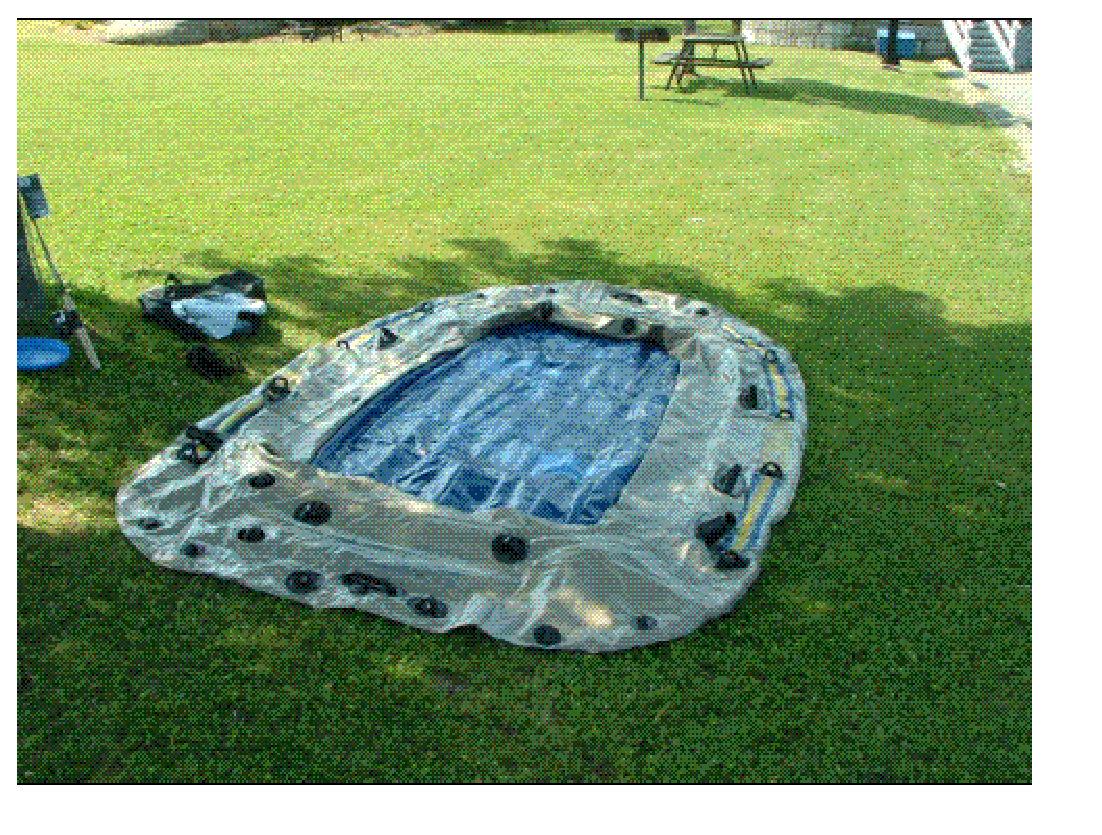
\epsfig{file=fig1.eps,width=3.5in}
Which one of the following is missing in it?
 
 
\noindent{\textbf{\large{
A.}}}
A frisbee
 
 
\noindent{\textbf{\large{
B.}}}
An air-boat
 
 
\noindent{\textbf{\large{
C.}}}
A truck
 
 
\noindent{\textbf{\large{
D.}}}
An airplane
 
 
\noindent{\textbf{\large{
E.}}}
A table
 
 
\noindent{\textbf{\large{
F.}}}
  Not any of aboves.
 
 
\noindent\vspace{0.05in}{\textbf{\Large{Auto-answer:}}}
 
 
\noindent{\textbf{\large{
C.}}}
A truck
 
 
\noindent{\textbf{\large{
D.}}}
An airplane
 
 
\noindent\vspace{0.05in}{\textbf{\Large{End of auto-answer.}}}
 
 
 
\vspace{0.3in}
   
   
\noindent{\textbf{\Large{Total numbers: }}}
   
   
\noindent\begin{tabular}{|l|l|l|l|l|l|l|}
 \hline
Inputs & Calculates & Choices & Layers & Matches & Answer & Solution \\ \hline
           0 & 
           0 & 
           6
  simple  
  & 
           6 & 
           0 & 
  yes & 
  no 
  \\ \hline
 \end{tabular}
   
   
   
   
\noindent\vspace{0.1in}{\textbf{\Large{Calculated values:}}}
   
   
   
   
\noindent\vspace{0.1in}\hspace{-0.08in} {\textbf{\Large{All inputs: }}}
   
   
   
   
\vspace{0.3in}
{\textbf{\LARGE{You have done all the above? A very good beginning, please go ahead.}}}
More constants the
Mass of electron
$m_e$$ =
9.109390 \times 10^{-31} $
kg
,
Universal gas constant
$R$$ =
8.315 $
J/(mol$\cdot $K)
,
$e$$ =
1.60217733 \times 10^{-19} $
C
, and
$m_p$$ =
1.6726231 \times 10^{-27} $
kg
%
may be very helpful.
\vspace{0.3in}
   
   
  
\vspace{0.2in}
  
{\textbf{\Large{QUESTION
26.2 
 (          1,          1,          1)
}}}
  
  


\noindent\vspace{0.05in}{\textbf{\Large{Abstract:}}}
This is a simple Newton's Second Law calculation multi-choice problem.  
\noindent\vspace{0.05in}{\textbf{\Large{end of abstract.}}}


 
 
An object is subjected to an external net force $\mathbf{f}=
(90.0 , 9.0 , -8000.0) N$.
Its mass is known as $m= % 
50.0000 kg$. Please choose the
correct accelaration from the following choices.
 
 
 
\noindent{\textbf{\large{
A.}}}
The accelaration is $  %
(
1.80,
.81,
-160.00)
ms^{-2} $.
 
 
\noindent{\textbf{\large{
B.}}}
The accelaration is $  %
(
4.24,
.81,
-160.00)
ms^{-2} $.
 
 
\noindent{\textbf{\large{
C.}}}
The accelaration is $  %
(
1.80,
.18,
-160.00)
ms^{-2} $.
 
 
\noindent{\textbf{\large{
D.}}}
The accelaration is $  %
(
4.24,
.18,
447.95)
ms^{-2} $.
 
 
\noindent{\textbf{\large{
E.}}}
The accelaration is $  %
(
4.24,
.18,
-160.00)
ms^{-2} $.
 
 
\noindent{\textbf{\large{
F.}}}
The accelaration is $  %
(
1.80,
.18,
447.95)
ms^{-2} $.
 
 
\noindent{\textbf{\large{
G.}}}
The accelaration is $  %
(
1.80,
.81,
447.95)
ms^{-2} $.
 
 
\noindent{\textbf{\large{
H.}}}
The accelaration is $  %
(
4.24,
.81,
447.95)
ms^{-2} $.
 
 
\noindent\vspace{0.05in}{\textbf{\Large{Auto-answer:}}}
 
 
\noindent{\textbf{\large{
C.}}}
The accelaration is $  %
(
1.80,
.18,
-160.00)
ms^{-2} $.
 
 
\noindent\vspace{0.05in}{\textbf{\Large{End of auto-answer.}}}
 
 
 
 
 
\noindent\vspace{0.05in}{\textbf{\Large{Answer:}}}
 
 

The correct answer from the choices is


\noindent{\textbf{\large{
C.}}}
The accelaration is $  %
(
1.80,
.18,
-160.00)
ms^{-2} $.
 
 
 
\noindent\vspace{0.05in}{\textbf{\Large{End of Answer.}}}
 
 

 
 
 
\noindent\vspace{0.1in}{\textbf{\Large{Solution: }}}
 
 

We will use the Newton's Second Law:
 
\[
\mathbf{f}=m\mathbf{a}.
\]
 
Since $\mathbf{f}= % 
(90.0 , 9.0 , -8000.0) N$
and $m= % 
50.0000kg$, bring them into the above equation, then we get
 
\begin{eqnarray*}
\mathbf{a}&=&\frac{\mathbf{f}}m  \\
&=&\frac{ % 
(90.0 , 9.0 , -8000.0) N}{ % 
50.0000kg}  \\
&=& % 
(1.80 , .18 , -160.00) ms^{-2}
\end{eqnarray*}
 
 
 
\noindent\vspace{0.1in}{\textbf{\Large{End of Solution.}}}
 
 

 
\vspace{0.3in}
   
   
\noindent{\textbf{\Large{Total numbers: }}}
   
   
\noindent\begin{tabular}{|l|l|l|l|l|l|l|}
 \hline
Inputs & Calculates & Choices & Layers & Matches & Answer & Solution \\ \hline
           2 & 
           1 & 
           8
  & 
           3 & 
           0 & 
  yes & 
  yes 
  \\ \hline
 \end{tabular}
   
   
   
   
\noindent\vspace{0.1in}{\textbf{\Large{Calculated values:}}}
   
   
  
  
\noindent\begin{tabular}{|l|l|l|l|}
\hline
 Sequential & Type & Accuracy & Calculated \\ 
\hline
 
 
  Calculated $           1$ & vector &  
  $           3 $ 
 &  $ 1.80 $ 
 \\    
  & & 
  $           2 $ 
 &  $ .18 $ 
 \\    
  & & 
  $           5 $ 
 &  $ -160.00 $ 
 \\  \hline  
 \end{tabular}
   
   
   
   
\noindent\vspace{0.1in}\hspace{-0.08in} {\textbf{\Large{All inputs: }}}
   
   
  
  
\noindent\begin{tabular}{|l|l|l|l|l|}
\hline
 Sequential & Type & Accuracy & Three inputs & Generated \\ 
\hline
 
 
  INPUT $           1$ & vector & $          -1 $ & $
20.0
  $ & \\
  & & & $
101.0
  $ & \\
  & & & $
10.0
$ & $ 90.0 $ 
  \\
  & & $          -1 $ & $
2.0
  $ & \\
  & & & $
10.1
  $ & \\
  & & & $
1.0
$ & $ 9.0 $ 
  \\
  & & $          -1 $ & $
-2000.0
  $ & \\
  & & & $
-10001.0
  $ & \\
  & & & $
-1000.0
$ & $ -8000.0 $ 
 \\  \hline  
 
 
  INPUT $           2$ & real & $          -4 $ & $
 50.0000
  $ & \\
  & & &  $
 60.1000
  $ & \\
  & & &  $
 2.0000
 $ & $ 50.0000 $ 
 \\  \hline  
 \end{tabular}
   
   
  
\vspace{0.2in}
  
{\textbf{\Large{QUESTION
26.3 
 (          2,          2,          2)
}}}
  
  
 
An object is subjected to an external net force $\mathbf{f}=(
80.000 ,
5.0000,
-9000.0  )N$. Its mass is known as
$m= % 
58.0000  kg$. Please choose the correct accelaration
from the following choices.
 
 
 
\noindent{\textbf{\large{
A.}}}
The accelaration is
$(
1.3793ms^{-2},
1117.2km/h^2,
-155.17ms^{-2}
).
$
 
 
\noindent{\textbf{\large{
B.}}}
The accelaration is
$(
5.7113ms^{-2},
3858.5km/h^2,
-155.17ms^{-2}
).
$
 
 
\noindent{\textbf{\large{
C.}}}
The accelaration is
$(
1.3793ms^{-2},
3858.5km/h^2,
533.37ms^{-2}
).
$
 
 
\noindent{\textbf{\large{
D.}}}
The accelaration is
$(
5.7113ms^{-2},
1117.2km/h^2,
533.37ms^{-2}
).
$
 
 
\noindent{\textbf{\large{
E.}}}
The accelaration is
$(
1.3793ms^{-2},
3858.5km/h^2,
-155.17ms^{-2}
).
$
 
 
\noindent{\textbf{\large{
F.}}}
The accelaration is
$(
1.3793ms^{-2},
1117.2km/h^2,
533.37ms^{-2}
).
$
 
 
\noindent{\textbf{\large{
G.}}}
 None of these.
 
 
\noindent\vspace{0.05in}{\textbf{\Large{Auto-answer:}}}
 
 
\noindent{\textbf{\large{
A.}}}
The accelaration is
$(
1.3793ms^{-2},
1117.2km/h^2,
-155.17ms^{-2}
).
$
 
 
\noindent\vspace{0.05in}{\textbf{\Large{End of auto-answer.}}}
 
 
 
 
 
 
\noindent\vspace{0.1in}{\textbf{\Large{Solution: }}}
 
 

We will use the Newton's Second Law:
 
\[
\mathbf{f}=m\mathbf{a}.
\]
 
Since $\mathbf{f}=( % 
80.000,  % 
5.0000,  % 
-9000.0 )N$
and $m= % 
58.0000kg$, bring them into the above equation, then we get
 
\begin{eqnarray*}
\mathbf{a}&=&\frac{\mathbf{f}}m  \\
&=&\frac{(
80.000 ,
5.0000 ,
-9000.0 )N
}{ % 
58.0000 kg}  \\
&=&(
1.3793 ,
8.6207 \times 10^{-2},
-155.17
)ms^{-2} \\
&=&(
17876. ,
1117.2 ,
-2.0110 \times 10^{6}
)km/h^2.
\end{eqnarray*}
 
 
 
\noindent\vspace{0.1in}{\textbf{\Large{End of Solution.}}}
 
 

 
\vspace{0.3in}
   
   
\noindent{\textbf{\Large{Total numbers: }}}
   
   
\noindent\begin{tabular}{|l|l|l|l|l|l|l|}
 \hline
Inputs & Calculates & Choices & Layers & Matches & Answer & Solution \\ \hline
           4 & 
           6 & 
           7
  & 
           3 & 
           0 & 
  yes & 
  yes 
  \\ \hline
 \end{tabular}
   
   
   
   
\noindent\vspace{0.1in}{\textbf{\Large{Calculated values:}}}
   
   
  
  
\noindent\begin{tabular}{|l|l|l|l|}
\hline
 Sequential & Type & Accuracy & Calculated \\ 
\hline
 
 
  Calculated $           1$ & real & $           5 $ & 
 $ 1.3793 $ 
 \\  \hline  
 
 
  Calculated $           2$ & real & $           5 $ & 
 $ 8.6207 \times 10^{-2} $ 
 \\  \hline  
 
 
  Calculated $           3$ & real & $           5 $ & 
 $ -155.17 $ 
 \\  \hline  
 
 
  Calculated $           4$ & real & $           5 $ & 
 $ 17876. $ 
 \\  \hline  
 
 
  Calculated $           5$ & real & $           5 $ & 
 $ 1117.2 $ 
 \\  \hline  
 
 
  Calculated $           6$ & real & $           5 $ & 
 $ -2.0110 \times 10^{6} $ 
 \\  \hline  
 \end{tabular}
   
   
   
   
\noindent\vspace{0.1in}\hspace{-0.08in} {\textbf{\Large{All inputs: }}}
   
   
  
  
\noindent\begin{tabular}{|l|l|l|l|l|}
\hline
 Sequential & Type & Accuracy & Three inputs & Generated \\ 
\hline
 
 
  INPUT $           1$ & real & $          -3 $ & $
 20.000
  $ & \\
  & & &  $
 101.000
  $ & \\
  & & &  $
 10.000
 $ & $ 80.000 $ 
 \\  \hline  
 
 
  INPUT $           2$ & real & $          -4 $ & $
 2.0000
  $ & \\
  & & &  $
 10.1000
  $ & \\
  & & &  $
 1.0000
 $ & $ 5.0000 $ 
 \\  \hline  
 
 
  INPUT $           3$ & real & $          -1 $ & $
 -2000.0
  $ & \\
  & & &  $
 -10001.0
  $ & \\
  & & &  $
 -1000.0
 $ & $ -9000.0 $ 
 \\  \hline  
 \end{tabular}
   
   
  
  
\noindent\begin{tabular}{|l|l|l|l|l|}
\hline
 Sequential & Type & Accuracy & Three inputs & Generated \\ 
\hline
 
 
  INPUT $           4$ & real & $          -4 $ & $
 50.0000
  $ & \\
  & & &  $
 60.1000
  $ & \\
  & & &  $
 2.0000
 $ & $ 58.0000 $ 
 \\  \hline  
 \end{tabular}
   
   
  
\vspace{0.2in}
  
{\textbf{\Large{QUESTION
26.4 
 (          3,          3,          3)
}}}
  
  
Please choose the correct one from the following statements:
 
 
\noindent{\textbf{\large{
A.}}}
Canada has  %
35 provinces and  %
34 territories.
 
 
\noindent{\textbf{\large{
B.}}}
Canada has  %
33 provinces and  %
38 territories.
 
 
\noindent{\textbf{\large{
C.}}}
Canada has  %
34 provinces and  %
39 territories.
 
 
\noindent{\textbf{\large{
D.}}}
Canada has  %
36 provinces and  %
35 territories.
 
 
\noindent{\textbf{\large{
E.}}}
Canada has  %
37 provinces and  %
37 territories.
 
 
\noindent{\textbf{\large{
F.}}}
 None of above.
 
 
\noindent\vspace{0.05in}{\textbf{\Large{Auto-answer:}}}
 
 
\noindent{\textbf{\large{
F.}}}
 None of above.
 
 
\noindent\vspace{0.05in}{\textbf{\Large{End of auto-answer.}}}
 
 
   
   
\noindent{\textbf{\Large{Total numbers: }}}
   
   
\noindent\begin{tabular}{|l|l|l|l|l|l|l|}
 \hline
Inputs & Calculates & Choices & Layers & Matches & Answer & Solution \\ \hline
           0 & 
          20 & 
           6
  simple  
  & 
           6 & 
           0 & 
  yes & 
  no 
  \\ \hline
 \end{tabular}
   
   
   
   
\noindent\vspace{0.1in}{\textbf{\Large{Calculated values:}}}
   
   
  
  
\noindent\begin{tabular}{|l|l|l|l|}
\hline
 Sequential & Type & Accuracy & Calculated \\ 
\hline
 
 
  Calculated $           1$ & integer &  & 
  $ 10 $ 
 \\  \hline  
 
 
  Calculated $           2$ & integer &  & 
  $ 3 $ 
 \\  \hline  
 
 
  Calculated $           3$ & integer &  & 
  $ 23 $ 
 \\  \hline  
 
 
  Calculated $           4$ & integer &  & 
  $ 24 $ 
 \\  \hline  
 
 
  Calculated $           5$ & integer &  & 
  $ 25 $ 
 \\  \hline  
 
 
  Calculated $           6$ & integer &  & 
  $ 26 $ 
 \\  \hline  
 
 
  Calculated $           7$ & integer &  & 
  $ 27 $ 
 \\  \hline  
 
 
  Calculated $           8$ & integer &  & 
  $ 28 $ 
 \\  \hline  
 
 
  Calculated $           9$ & integer &  & 
  $ 29 $ 
 \\  \hline  
 
 
  Calculated $          10$ & integer &  & 
  $ 30 $ 
 \\  \hline  
 \end{tabular}
   
   
  
  
\noindent\begin{tabular}{|l|l|l|l|}
\hline
 Sequential & Type & Accuracy & Calculated \\ 
\hline
 
 
  Calculated $          11$ & integer &  & 
  $ 31 $ 
 \\  \hline  
 
 
  Calculated $          12$ & integer &  & 
  $ 32 $ 
 \\  \hline  
 
 
  Calculated $          13$ & integer &  & 
  $ 33 $ 
 \\  \hline  
 
 
  Calculated $          14$ & integer &  & 
  $ 34 $ 
 \\  \hline  
 
 
  Calculated $          15$ & integer &  & 
  $ 35 $ 
 \\  \hline  
 
 
  Calculated $          16$ & integer &  & 
  $ 36 $ 
 \\  \hline  
 
 
  Calculated $          17$ & integer &  & 
  $ 37 $ 
 \\  \hline  
 
 
  Calculated $          18$ & integer &  & 
  $ 38 $ 
 \\  \hline  
 
 
  Calculated $          19$ & integer &  & 
  $ 39 $ 
 \\  \hline  
 
 
  Calculated $          20$ & integer &  & 
  $ 40 $ 
 \\  \hline  
 \end{tabular}
   
   
   
   
\noindent\vspace{0.1in}\hspace{-0.08in} {\textbf{\Large{All inputs: }}}
   
   
  
\vspace{0.2in}
  
{\textbf{\Large{QUESTION
26.5 
 (          5,          5,          5)
}}}
  
  
If any one of the following statements is correct, please fill the box ahead of it with $T$ .
If wrong, fill with $F$.
 
\noindent\begin{tabular}{|l|l|}\hline Your&\hspace{.2in} \\ answer&\hspace{.2in} \\ \hline \end{tabular}
1. $ % 
78$ is an  % 
odd number.
 
\noindent\begin{tabular}{|l|l|}\hline Your&\hspace{.2in} \\ answer&\hspace{.2in} \\ \hline \end{tabular}
2.  % 
Toronto is in  % 
Ontario province.
 
\noindent\begin{tabular}{|l|l|}\hline Your&\hspace{.2in} \\ answer&\hspace{.2in} \\ \hline \end{tabular}
3.  % 
$\mathbf{F}=m\mathbf{a}$ is a mathmatical form of
Newton's Law of Universal Gravitation.
 
 
 
\noindent\vspace{0.05in}{\textbf{\Large{Answer:}}}
 
 

 
\noindent\begin{tabular}{|l|l|}\hline The correct & \\
          answer &  % 
$F$ \\ \hline \end{tabular}
1. $ % 
78$ is an  % 
odd number.
 
\noindent\begin{tabular}{|l|l|}\hline The correct & \\
          answer &  % 
$T$ \\ \hline \end{tabular}
2.  % 
Toronto is in  % 
Ontario province.
 
\noindent\begin{tabular}{|l|l|}\hline The correct & \\
          answer &  % 
$F$ \\ \hline \end{tabular}
3.  % 
$\mathbf{F}=m\mathbf{a}$ is a mathmatical form of  % 
Newton's Law of Universal Gravitation.
 
 
 
\noindent\vspace{0.05in}{\textbf{\Large{End of Answer.}}}
 
 

 
\vspace{0.3in}
   
   
\noindent{\textbf{\Large{Total numbers: }}}
   
   
\noindent\begin{tabular}{|l|l|l|l|l|l|l|}
 \hline
Inputs & Calculates & Choices & Layers & Matches & Answer & Solution \\ \hline
           6 & 
           3 & 
           0
  & 
           0 & 
           0 & 
  yes & 
  no 
  \\ \hline
 \end{tabular}
   
   
   
   
\noindent\vspace{0.1in}{\textbf{\Large{Calculated values:}}}
   
   
  
  
\noindent\begin{tabular}{|l|l|l|l|}
\hline
 Sequential & Type & Accuracy & Calculated \\ 
\hline
 
 
  Calculated $           1$ & string & $           2 $ ( $          2 $ strings)
 : 
 & $F$
 \\  \hline  
 
 
  Calculated $           2$ & string & $           1 $ ( $          2 $ strings)
 : 
 & $T$
 \\  \hline  
 
 
  Calculated $           3$ & string & $           2 $ ( $          2 $ strings)
 : 
 & $F$
 \\  \hline  
 \end{tabular}
   
   
   
   
\noindent\vspace{0.1in}\hspace{-0.08in} {\textbf{\Large{All inputs: }}}
   
   
  
  
\noindent\begin{tabular}{|l|l|l|l|l|}
\hline
 Sequential & Type & Accuracy & Three inputs & Generated \\ 
\hline
 
 
  INPUT $           1$ & integer &  & $
 1
 , 
 100
 , 
 1
 $ & $ 78 $ 
 \\  \hline  
 
 
  INPUT $           2$ & string & & 
 even & 
  \\
  & & & 
 odd & 
  $ <-- $ 
 \\  \hline  
 
 
  INPUT $           3$ & string & & 
 Toronto & 
  $ <-- $ 
  \\
  & & & 
 Kingston & 
  \\
  & & & 
 Montreal & 
  \\
  & & & 
 Hull & 
 \\  \hline  
 \end{tabular}
   
   
  
  
\noindent\begin{tabular}{|l|l|l|l|l|}
\hline
 Sequential & Type & Accuracy & Three inputs & Generated \\ 
\hline
 
 
  INPUT $           4$ & string & & 
 Ontario & 
  $ <-- $ 
  \\
  & & & 
 Quebec & 
 \\  \hline  
 
 
  INPUT $           5$ & string & & 
 $\mathbf{F}=m\mathbf{a}$ & 
  $ <-- $ 
  \\
  & & & 
 $\left| \mathbf{F}\right| =Gm_1m_2r^{-2}$ & 
 \\  \hline  
 
 
  INPUT $           6$ & string & & 
 the Newton's Second Law & 
  \\
  & & & 
 Newton's Law of Universal Gravitation & 
  $ <-- $ 
 \\  \hline  
 \end{tabular}
   
   
  
\vspace{0.2in}
  
{\textbf{\Large{QUESTION
26.6 
 (          4,          4,          4)
}}}
  
  
Considering case-insensitivity, please match the following same strings.
  
  
\begin{tabular}{|l|l|l|}
 \hline
 Column Left & Column Right  & Your choinces \\ 
 \hline
{\textbf{\large{
A.}}}
er
  & 
ASDF(:)
 & 
 \\ 
 \hline
{\textbf{\large{
B.}}}
Er
  & 
b
 & 
 \\ 
 \hline
{\textbf{\large{
C.}}}
B
  & 
eR
 & 
 \\ 
 \hline
{\textbf{\large{
D.}}}
asdf(:)
  & 
a
 & 
 \\ 
 \hline
{\textbf{\large{
E.}}}
A
  & 
ER
 & 
 \\ 
 \hline
 \end{tabular}
  
  
 
 
\noindent\vspace{0.05in}{\textbf{\Large{Auto-answer:}}}
  
  
\begin{tabular}{|l|l|l|}
 \hline
 Column Left & Column Right  & Answers       \\ 
 \hline
{\textbf{\large{
A.}}}
er
  & 
ASDF(:)
 & 
{\textbf{\large{
D.}}}
 \\ 
 \hline
{\textbf{\large{
B.}}}
Er
  & 
b
 & 
{\textbf{\large{
C.}}}
 \\ 
 \hline
{\textbf{\large{
C.}}}
B
  & 
eR
 & 
{\textbf{\large{
A.}}}
, 
{\textbf{\large{
B.}}}
 \\ 
 \hline
{\textbf{\large{
D.}}}
asdf(:)
  & 
a
 & 
{\textbf{\large{
E.}}}
 \\ 
 \hline
{\textbf{\large{
E.}}}
A
  & 
ER
 & 
{\textbf{\large{
A.}}}
, 
{\textbf{\large{
B.}}}
 \\ 
 \hline
 \end{tabular}
  
  
 
 
\noindent\vspace{0.05in}{\textbf{\Large{End of auto-answer.}}}
 
 
 
   
   
\noindent{\textbf{\Large{Total numbers: }}}
   
   
\noindent\begin{tabular}{|l|l|l|l|l|l|l|}
 \hline
Inputs & Calculates & Choices & Layers & Matches & Answer & Solution \\ \hline
           2 & 
           1 & 
           0
  & 
          16 & 
           5 & 
  yes & 
  no 
  \\ \hline
 \end{tabular}
   
   
   
   
\noindent\vspace{0.1in}{\textbf{\Large{Calculated values:}}}
   
   
  
  
\noindent\begin{tabular}{|l|l|l|l|}
\hline
 Sequential & Type & Accuracy & Calculated \\ 
\hline
 
 
  Calculated $           1$ & integer &  & 
  $ 4 $ 
 \\  \hline  
 \end{tabular}
   
   
   
   
\noindent\vspace{0.1in}\hspace{-0.08in} {\textbf{\Large{All inputs: }}}
   
   
  
  
\noindent\begin{tabular}{|l|l|l|l|l|}
\hline
 Sequential & Type & Accuracy & Three inputs & Generated \\ 
\hline
 
 
  INPUT $           1$ & integer &  & $
 2
 , 
 8
 , 
 2
 $ & $ 8 $ 
 \\  \hline  
 
 
  INPUT $           2$ & integer &  & $
 2
 , 
 3
 , 
 2
 $ & $ 2 $ 
 \\  \hline  
 \end{tabular}
   
   
   
   
\vspace{0.3in}
{\textbf{\LARGE{You have done all the above? Excellent! Not much left, please continue.}}}
\vspace{0.3in}
   
   
  
\vspace{0.2in}
  
{\textbf{\Large{QUESTION
26.7 
 (          7,         14,         50)
}}}
  
  
 
An object is subjected to an external net force $\mathbf{f}=
(90.0 , 7.0 , -7000.0) N$.
Its mass is known as $m= % 
58.0 kg$.
Please choose the correct accelaration from the following choices.
 
 
\noindent{\textbf{\large{
A.}}}
  The accelaration is $  %
(
1.55,
.12,
-120.69)
ms^{-2} $.
 
 
\noindent{\textbf{\large{
B.}}}
  The accelaration is $  %
(
-3.12,
.39,
-120.69)
ms^{-2} $.
 
 
\noindent{\textbf{\large{
C.}}}
  The accelaration is $  %
(
1.55,
.39,
-120.69)
ms^{-2} $.
 
 
\noindent{\textbf{\large{
D.}}}
  The accelaration is $  %
(
-3.12,
.12,
-120.69)
ms^{-2} $.
 
 
\noindent\vspace{0.05in}{\textbf{\Large{Auto-answer:}}}
 
 
\noindent{\textbf{\large{
A.}}}
  The accelaration is $  %
(
1.55,
.12,
-120.69)
ms^{-2} $.
 
 
\noindent\vspace{0.05in}{\textbf{\Large{End of auto-answer.}}}
 
 
 
 
 
\noindent\vspace{0.1in}{\textbf{\Large{Solution: }}}
 
 

We will use the Newton's Second Law:
 
\[
\mathbf{f}=m\mathbf{a}.
\]
 
Since $\mathbf{f}= % 
(90.0 , 7.0 , -7000.0) N$
and $m= % 
58.0kg$, bring them into the above equation, then we get
 
\begin{eqnarray*}
\mathbf{a}&=&\frac{\mathbf{f}}m  \\
&=&\frac{ % 
(90.0 , 7.0 , -7000.0) N}{ % 
58.0kg}  \\
&=& % 
(1.55 , .12 , -120.69) ms^{-2}
\end{eqnarray*}
 
 
 
\noindent\vspace{0.1in}{\textbf{\Large{End of Solution.}}}
 
 

 
 
\vspace{0.3in}
   
   
\noindent{\textbf{\Large{Total numbers: }}}
   
   
\noindent\begin{tabular}{|l|l|l|l|l|l|l|}
 \hline
Inputs & Calculates & Choices & Layers & Matches & Answer & Solution \\ \hline
           2 & 
           1 & 
           4
  & 
           3 & 
           0 & 
  yes & 
  yes 
  \\ \hline
 \end{tabular}
   
   
   
   
\noindent\vspace{0.1in}{\textbf{\Large{Calculated values:}}}
   
   
  
  
\noindent\begin{tabular}{|l|l|l|l|}
\hline
 Sequential & Type & Accuracy & Calculated \\ 
\hline
 
 
  Calculated $           1$ & vector &  
  $           3 $ 
 &  $ 1.55 $ 
 \\    
  & & 
  $           2 $ 
 &  $ .12 $ 
 \\    
  & & 
  $           5 $ 
 &  $ -120.69 $ 
 \\  \hline  
 \end{tabular}
   
   
   
   
\noindent\vspace{0.1in}\hspace{-0.08in} {\textbf{\Large{All inputs: }}}
   
   
  
  
\noindent\begin{tabular}{|l|l|l|l|l|}
\hline
 Sequential & Type & Accuracy & Three inputs & Generated \\ 
\hline
 
 
  INPUT $           1$ & vector & $          -1 $ & $
20.0
  $ & \\
  & & & $
101.0
  $ & \\
  & & & $
10.0
$ & $ 90.0 $ 
  \\
  & & $          -1 $ & $
2.0
  $ & \\
  & & & $
10.1
  $ & \\
  & & & $
1.0
$ & $ 7.0 $ 
  \\
  & & $          -1 $ & $
-2000.0
  $ & \\
  & & & $
-10001.0
  $ & \\
  & & & $
-1000.0
$ & $ -7000.0 $ 
 \\  \hline  
 
 
  INPUT $           2$ & real & $          -1 $ & $
 50.0
  $ & \\
  & & &  $
 60.1
  $ & \\
  & & &  $
 2.0
 $ & $ 58.0 $ 
 \\  \hline  
 \end{tabular}
   
   
  
\vspace{0.2in}
  
{\textbf{\Large{QUESTION
26.8 
 (          8,         15,         60)
}}}
  
  
 
$ \left( \begin{array}{ccccccccc}
           4 & 
           7 & 
           5 & 
           6 \\ 
           6 & 
           6 & 
           7 & 
           5 \\ 
           4 & 
           4 & 
           4 & 
           4
\end{array}\right) \times
\left( \begin{array}{c}
           2 \\ 
           2 \\ 
           2 \\ 
           2
\end{array}\right) $ =?
 
 
$  % 
 \left( \begin{array}
 {
 c
 c
 }
 \varepsilon & 
 \rho \\ 
 \sigma & 
 \beta \\ 
 \Lambda & 
 \Delta \\ 
 \Omega & 
                    \Xi
 \end{array} \right)
 \left( \begin{array}
 {
 c
 }
 \gamma \\ 
 \gamma
 \end{array} \right)
$ =?
 
 
 
\noindent\vspace{0.05in}{\textbf{\Large{Answer:}}}
 
 

 
$\left( \begin{array}{ccccccccccccccc}
           4 & 
           7 & 
           5 & 
           6 \\ 
           6 & 
           6 & 
           7 & 
           5 \\ 
           4 & 
           4 & 
           4 & 
           4
\end{array}\right) \times
\left( \begin{array}{c}
           2 \\ 
           2 \\ 
           2 \\ 
           2
\end{array}\right)  =
\left( \begin{array}{c}
          44 \\ 
          48 \\ 
          32
\end{array}\right)  $
 
$  % 
 \left( \begin{array}
 {
 c
 c
 }
 \varepsilon & 
 \rho \\ 
 \sigma & 
 \beta \\ 
 \Lambda & 
 \Delta \\ 
 \Omega & 
                    \Xi
 \end{array} \right)
 \left( \begin{array}
 {
 c
 }
 \gamma \\ 
 \gamma
 \end{array} \right)
=
  \left( \begin{array}
 {
 c
 }
 \varepsilon \times  \gamma   +  \rho \times  \gamma \\ 
 \sigma \times  \gamma   +  \beta \times  \gamma \\ 
 \Lambda \times  \gamma   +  \Delta \times  \gamma \\ 
 \Omega \times  \gamma   +                     \Xi \times  \gamma
 \end{array} \right)
$
 
 
 
\noindent\vspace{0.05in}{\textbf{\Large{End of Answer.}}}
 
 

 
 
 
\noindent\vspace{0.1in}{\textbf{\Large{Solution: }}}
 
 

 
 
\noindent\vspace{0.1in}{\textbf{\Large{End of Solution.}}}
 
 

 
\vspace{0.3in}
   
   
\noindent{\textbf{\Large{Total numbers: }}}
   
   
\noindent\begin{tabular}{|l|l|l|l|l|l|l|}
 \hline
Inputs & Calculates & Choices & Layers & Matches & Answer & Solution \\ \hline
           4 & 
           2 & 
           0
  & 
           0 & 
           0 & 
  yes & 
  yes 
  \\ \hline
 \end{tabular}
   
   
   
   
\noindent\vspace{0.1in}{\textbf{\Large{Calculated values:}}}
   
   
  
  
\noindent\begin{tabular}{|l|l|l|l|}
\hline
 Sequential & Type & Accuracy & Calculated \\ 
\hline
 
 
  Calculated $           1$ & i-matrix &  & 
 (size:           3 by           1)
 \\  \hline  
 \end{tabular}
   
   
$\begin{array}{
 c
 }
          44 \\ 
          48 \\ 
          32
 \end{array}  $ 
  
  
\noindent\begin{tabular}{|l|l|l|l|}
\hline
 Sequential & Type & Accuracy & Calculated \\ 
\hline
 
 
  Calculated $           2$ & s-matrix & & 
 (size:           4 by           1)
 \\  \hline  
 \end{tabular}
   
   
 $   \left( \begin{array}
 {
 c
 }
 \varepsilon \times  \gamma   +  \rho \times  \gamma \\ 
 \sigma \times  \gamma   +  \beta \times  \gamma \\ 
 \Lambda \times  \gamma   +  \Delta \times  \gamma \\ 
 \Omega \times  \gamma   +                     \Xi \times  \gamma
 \end{array} \right) $ 
   
   
\noindent\vspace{0.1in}\hspace{-0.08in} {\textbf{\Large{All inputs: }}}
   
   
  
  
\noindent\begin{tabular}{|l|l|l|l|l|}
\hline
 Sequential & Type & Accuracy & Three inputs & Generated \\ 
\hline
 
 
  INPUT $           1$ & i-matrix &  & $
 4
 , 
 7
 , 
 1
 $ & (size:           3 by           4)
 \\  \hline  
 \end{tabular}
   
   
 $\begin{array}{
 c
 c
 c
 c
 }
           4 & 
           7 & 
           5 & 
           6 \\ 
           6 & 
           6 & 
           7 & 
           5 \\ 
           4 & 
           4 & 
           4 & 
           4
\end{array}  $ 
  
  
\noindent\begin{tabular}{|l|l|l|l|l|}
\hline
 Sequential & Type & Accuracy & Three inputs & Generated \\ 
\hline
 
 
  INPUT $           2$ & i-matrix &  & $
 2
 , 
 2
 , 
 1
 $ & (size:           4 by           1)
 \\  \hline  
 \end{tabular}
   
   
 $\begin{array}{
 c
 }
           2 \\ 
           2 \\ 
           2 \\ 
           2
\end{array}  $ 
  
  
\noindent\begin{tabular}{|l|l|l|l|l|}
\hline
 Sequential & Type & Accuracy & Three inputs & Generated \\ 
\hline
 
 
  INPUT $           3$ & s-matrix & & 
 $  \alpha $ & 
  \\
  & & & 
 $  \beta $ & 
  \\
  & & & 
 $  \gamma $ & 
  \\
  & & & 
 $  \delta $ & 
  \\
  & & & 
 $  \epsilon $ & 
  \\
  & & & 
 $  \varepsilon $ & 
  \\
  & & & 
 $                     \zeta $ & 
  \\
  & & & 
 $  \eta $ & 
  \\
  & & & 
 $  \rho $ & 
  \\
  & & & 
 $  \sigma $ & 
  \\
  & & & 
 $  \Gamma $ & 
  \\
  & & & 
 $  \Delta $ & 
  \\
  & & & 
 $  \Theta $ & 
  \\
  & & & 
 $  \Lambda $ & 
  \\
  & & & 
 $                     \Xi $ & 
  \\
  & & & 
 $  \Upsilon $ & 
  \\
  & & & 
 $  \Phi $ & 
  \\
  & & & 
 $  \Psi $ & 
  \\
  & & & 
 $  \Omega $ & 
  (size:           4 by           2)
 \\  \hline  
 \end{tabular}
   
   
 $  \left( \begin{array}
 {
 c
 c
 }
 \varepsilon & 
 \rho \\ 
 \sigma & 
 \beta \\ 
 \Lambda & 
 \Delta \\ 
 \Omega & 
                    \Xi
 \end{array} \right) $ 
  
  
\noindent\begin{tabular}{|l|l|l|l|l|}
\hline
 Sequential & Type & Accuracy & Three inputs & Generated \\ 
\hline
 
 
  INPUT $           4$ & s-matrix & & 
 $  \beta $ & 
  \\
  & & & 
 $  \gamma $ & 
  (size:           2 by           1)
 \\  \hline  
 \end{tabular}
   
   
 $  \left( \begin{array}
 {
 c
 }
 \gamma \\ 
 \gamma
 \end{array} \right) $ 
  
\vspace{0.2in}
  
{\textbf{\Large{QUESTION
26.9 
 (          9,         16,         70)
}}}
  
  


\noindent\vspace{0.05in}{\textbf{\Large{Abstract:}}}
Quadratic Equation constructed from the following first two random (input) integers as roots,  
which of course should not show in the exam papers.  
\noindent\vspace{0.05in}{\textbf{\Large{end of abstract.}}}


 
 
% First root
% Second root

 
Please solve the following equation:
\begin{eqnarray*}
7 \times x^2  % 
-28
                 \times x    % 
-539 =0
\end{eqnarray*}
 
 
 
\noindent\vspace{0.05in}{\textbf{\Large{Answer:}}}
 
 

-7,  % 
11
 
 
 
\noindent\vspace{0.05in}{\textbf{\Large{End of Answer.}}}
 
 

 
 
 
\noindent\vspace{0.1in}{\textbf{\Large{Solution: }}}
 
 

Roots to the equation
\begin{eqnarray*}
7 \times x^2  % 
-28
                 \times x    % 
-539 =0
\end{eqnarray*}
are  % 
-7 and  % 
11 .
 
Let us verity  % 
-7 first:
$  % 
7 \times x^2  % 
-28
                 \times x    % 
-539
  = % 
343+( % 
196)+( % 
-539)
  = % 
539+( % 
-539)
  = % 
0
$
 
Then verity  % 
11:
$  % 
7 \times x^2  % 
-28
                 \times x    % 
-539
  = % 
847+( % 
-308)+( % 
-539)
  = % 
539+( % 
-539)
  = % 
0
$
 
 
 
\noindent\vspace{0.1in}{\textbf{\Large{End of Solution.}}}
 
 

 
\vspace{0.3in}
   
   
\noindent{\textbf{\Large{Total numbers: }}}
   
   
\noindent\begin{tabular}{|l|l|l|l|l|l|l|}
 \hline
Inputs & Calculates & Choices & Layers & Matches & Answer & Solution \\ \hline
           3 & 
          13 & 
           0
  & 
           0 & 
           0 & 
  yes & 
  yes 
  \\ \hline
 \end{tabular}
   
   
   
   
\noindent\vspace{0.1in}{\textbf{\Large{Calculated values:}}}
   
   
  
  
\noindent\begin{tabular}{|l|l|l|l|}
\hline
 Sequential & Type & Accuracy & Calculated \\ 
\hline
 
 
  Calculated $           1$ & integer &  & 
  $ 7 $ 
 \\  \hline  
 
 
  Calculated $           2$ & string & $           2 $ ( $          2 $ strings)
 : 
 & 
 \\  \hline  
 
 
  Calculated $           3$ & integer &  & 
  $ -28 $ 
 \\  \hline  
 
 
  Calculated $           4$ & string & $           2 $ ( $          2 $ strings)
 : 
 & 
 \\  \hline  
 
 
  Calculated $           5$ & integer &  & 
  $ -539 $ 
 \\  \hline  
 
 
  Calculated $           6$ & integer &  & 
  $ 343 $ 
 \\  \hline  
 
 
  Calculated $           7$ & integer &  & 
  $ 196 $ 
 \\  \hline  
 
 
  Calculated $           8$ & integer &  & 
  $ 539 $ 
 \\  \hline  
 
 
  Calculated $           9$ & integer &  & 
  $ 0 $ 
 \\  \hline  
 
 
  Calculated $          10$ & integer &  & 
  $ 847 $ 
 \\  \hline  
 \end{tabular}
   
   
  
  
\noindent\begin{tabular}{|l|l|l|l|}
\hline
 Sequential & Type & Accuracy & Calculated \\ 
\hline
 
 
  Calculated $          11$ & integer &  & 
  $ -308 $ 
 \\  \hline  
 
 
  Calculated $          12$ & integer &  & 
  $ 539 $ 
 \\  \hline  
 
 
  Calculated $          13$ & integer &  & 
  $ 0 $ 
 \\  \hline  
 \end{tabular}
   
   
   
   
\noindent\vspace{0.1in}\hspace{-0.08in} {\textbf{\Large{All inputs: }}}
   
   
  
  
\noindent\begin{tabular}{|l|l|l|l|l|}
\hline
 Sequential & Type & Accuracy & Three inputs & Generated \\ 
\hline
 
 
  INPUT $           1$ & integer &  & $
 -11
 , 
 30
 , 
 4
 $ & $ -7 $ 
 \\  \hline  
 
 
  INPUT $           2$ & integer &  & $
 -31
 , 
 60
 , 
 3
 $ & $ 11 $ 
 \\  \hline  
 
 
  INPUT $           3$ & integer &  & $
 -15
 , 
 15
 , 
 2
 $ & $ 7 $ 
 \\  \hline  
 \end{tabular}
   
   
   
   
   
   
 \vspace{0.2in}
Here are still some constants for use:
 
 
\noindent\begin{tabular}{|l|l|l|}
\hline
Constant & Symbol & Value \\
\hline
 
Mass of proton &
$m_p$ &
 $ 1.6726231 \times 10^{-27} $
kg \\
\hline
 
Boltzmann's constant &
$k$ &
 $ 1.381 \times 10^{-23} $
J/K \\
\hline
 
\end{tabular}
 
Thank you very much for answering these questions!
 
{\textbf{\large{Please be advised}}} that in this paper there are questions from
26.1 through
26.9.
And any one of them may contain more than one sub-question, thus the total number
of sub-questions here is around 14, of which
13 should be answered.
 
   
   
\vspace{2.0in} PAPER TAIL GENERATED.
   
   
   
   
\vspace{1.0in} 
{\textbf{\large{ *** END OF PAPER, THANKS *** }}} 
   
   
\hspace{1.0in} By: 
         239(         26,          34)
   
   
   
   
\newpage 
\setcounter{page}{ 
    27001 } 
   
   
\noindent{\textbf{\huge{THIS IS THE JOURNAL FOR}}}
   
   
 {\textbf{ \Large{ PAPER NUMBER          27 }}}
   
   
\vspace{0.2in}
   
   
\markboth{Journal NOT for examinees !!! {\today}}{Journal NOT for examinees !!! {\today}}
   
   
   
   
   
   
 \vspace{0.2in}
 
 
{\Huge  THIS IS AN EXAMPLE OF}
 
{\Huge  PERSONALIZED TESTS. }
 
If needed, please use the following constants.
 
 
 
\noindent\begin{tabular}{|l|l|l|}
\hline
Constant & Symbol & Value \\
\hline
Acceleration due to earth's gravity &
$g$ &
 $ 9.80 $
m/s$^2$ \\
\hline
Avogadro's number &
$N_A$ &
 $ 6.0221367 \times 10^{23} $
mol$^{-1}$ \\
\hline
Boltzmann's constant &
$k$ &
 $ 1.380658 \times 10^{-23} $
J/K \\
\hline
Coulomb's constant &
$k$ &
 $ 8.99 \times 10^{9} $
N$\cdot $m$^2$/C$^2$ \\
\hline
Electron charge magnitiude &
$e$ &
 $ 1.60217733 \times 10^{-19} $
C \\
\hline
Permeability of free space &
$\mu _0$ &
 $ 1.25663706 \times 10^{-6} $
T$\cdot $m/A \\
\hline
Permittivity of free space &
$\epsilon _0$ &
 $ 8.854187817 \times 10^{-12} $
C$^2$/(N$\cdot $m$^2$) \\
\hline
Pi &
$\pi$ &
 $ 3.14159265 $
$ $ \\
\hline
Planck's constant &
$h$ &
 $ 6.6260755 \times 10^{-34} $
J$\cdot $s \\
\hline
Mass of electron &
$m_e$ &
 $ 9.1093897 \times 10^{-31} $
kg \\
\hline
\end{tabular}
 
 
\noindent\begin{tabular}{|l|l|l|}
\hline
Constant & Symbol & Value \\
\hline
Mass of neutron &
$m_n$ &
 $ 1.6749286 \times 10^{-27} $
kg \\
\hline
Mass of proton &
$m_p$ &
 $ 1.6726231 \times 10^{-27} $
kg \\
\hline
Speed of light in vacuum &
$c$ &
 $ 299792458. $
m/s \\
\hline
Universal gravitational constant &
$G$ &
 $ 6.67259 \times 10^{-11} $
N$\cdot $m$^2$/kg$^2$ \\
\hline
Universal gas constant &
$R$ &
 $ 8.314510 $
J/(mol$\cdot $K) \\
\hline
\end{tabular}
 
 
{\textbf{\large{Please be advised}}} that in this paper there are questions from
27.1 through
27.9.
And any one of them may contain more than one sub-question, thus the total number
of sub-questions here is around 14, of which
13 should be answered.
 
\vspace{0.3in}
 
 
   
   
 PAPER TITLE GENERATED.
   
   
   
\vspace{0.2in}
   
In this paper, big questions will be generated in the following order: 
   
   
            1(          6)
 ,
            2(          4)
 ,
            3(          3)
 ,
            4(          2)
 ,
            5(          1)
 ,
            6(          5)
 ,
            7(          8)
 ,
            8(          7)
 ,
            9(          9)
 .
  
\vspace{0.2in}
  
{\textbf{\Large{QUESTION
27.1 
 (          6)
}}}
  
  
 
{\textbf{\Large{Please answer ONLY
5 of the following
6 questions (Questions
27.1.1 through
27.1.6). }}}
 
Here are still some constants for use in the following questions:
 
 
\noindent\begin{tabular}{|l|l|l|}
\hline
Constant & Symbol & Value \\
\hline
 
Boltzmann's constant &
$k$ &
 $ 1.381 \times 10^{-23} $
J/K \\
\hline
 
Avogadro's number &
$N_A$ &
 $ 6.022 \times 10^{23} $
mol$^{-1}$ \\
\hline
 
Mass of electron &
$m_e$ &
 $ 9.1093897 \times 10^{-31} $
kg \\
\hline
 
\end{tabular}
 
   
\vspace{0.2in}
   
 In this big question of CHOOSE structure,           6 questions will be generat
 ed: 
  
  
            1(          8,         23)
 ,
            2(         10,         25)
 ,
            3(          6,         21)
 ,
            4(         11,         26)
 ,
            5(         13,         28)
 ,
            6(          7,         22)
 .
  
\vspace{0.2in}
  
{\textbf{\Large{Question
27.1.1 
 (          6,          8,         23)
}}}
  
  
 
An object is subjected to an external net force $\mathbf{f}=(
90.0 ,
6.0,
-3000.0  )N$. Its mass is known as
$m= % 
52.0  kg$. Please choose the correct accelaration
from the following choices.
 
 
 
\noindent{\textbf{\large{
A.}}}
The accelaration is
$(
1.7308ms^{-2},
.54163ms^{-2},
-747692.km/h^2
).
$
 
 
\noindent{\textbf{\large{
B.}}}
The accelaration is
$(
4.9623ms^{-2},
.54163ms^{-2},
3.3972 \times 10^{6}km/h^2
).
$
 
 
\noindent{\textbf{\large{
C.}}}
The accelaration is
$(
1.7308ms^{-2},
.54163ms^{-2},
3.3972 \times 10^{6}km/h^2
).
$
 
 
\noindent{\textbf{\large{
D.}}}
The accelaration is
$(
4.9623ms^{-2},
.11538ms^{-2},
3.3972 \times 10^{6}km/h^2
).
$
 
 
\noindent{\textbf{\large{
E.}}}
none of these.
 
 
\noindent\vspace{0.05in}{\textbf{\Large{Auto-answer:}}}
 
 
\noindent{\textbf{\large{
E.}}}
none of these.
 
 
\noindent\vspace{0.05in}{\textbf{\Large{End of auto-answer.}}}
 
 
 
 
 
 
\noindent\vspace{0.1in}{\textbf{\Large{Solution: }}}
 
 

We will use the Newton's Second Law:
 
\[
\mathbf{f}=m\mathbf{a}.
\]
 
Since $\mathbf{f}=( % 
90.0,  % 
6.0,  % 
-3000.0 )N$
and $m= % 
52.0kg$, bring them into the above equation, then we get
 
\begin{eqnarray*}
\mathbf{a}&=&\frac{\mathbf{f}}m  \\
&=&\frac{(
90.0 ,
6.0 ,
-3000.0 )N
}{ % 
52.0 kg}  \\
&=&(
1.7308 ,
.11538,
-57.692
)ms^{-2} \\
&=&(
22431. ,
1495.4 ,
-747692.
)km/h^2.
\end{eqnarray*}
 
 
 
\noindent\vspace{0.1in}{\textbf{\Large{End of Solution.}}}
 
 

 
\vspace{0.3in}
   
   
\noindent{\textbf{\Large{Total numbers: }}}
   
   
\noindent\begin{tabular}{|l|l|l|l|l|l|l|}
 \hline
Inputs & Calculates & Choices & Layers & Matches & Answer & Solution \\ \hline
           4 & 
           6 & 
           5
  & 
           3 & 
           0 & 
  yes & 
  yes 
  \\ \hline
 \end{tabular}
   
   
   
   
\noindent\vspace{0.1in}{\textbf{\Large{Calculated values:}}}
   
   
  
  
\noindent\begin{tabular}{|l|l|l|l|}
\hline
 Sequential & Type & Accuracy & Calculated \\ 
\hline
 
 
  Calculated $           1$ & real & $           5 $ & 
 $ 1.7308 $ 
 \\  \hline  
 
 
  Calculated $           2$ & real & $           5 $ & 
 $ .11538 $ 
 \\  \hline  
 
 
  Calculated $           3$ & real & $           5 $ & 
 $ -57.692 $ 
 \\  \hline  
 
 
  Calculated $           4$ & real & $           5 $ & 
 $ 22431. $ 
 \\  \hline  
 
 
  Calculated $           5$ & real & $           5 $ & 
 $ 1495.4 $ 
 \\  \hline  
 
 
  Calculated $           6$ & real & $           5 $ & 
 $ -747692. $ 
 \\  \hline  
 \end{tabular}
   
   
   
   
\noindent\vspace{0.1in}\hspace{-0.08in} {\textbf{\Large{All inputs: }}}
   
   
  
  
\noindent\begin{tabular}{|l|l|l|l|l|}
\hline
 Sequential & Type & Accuracy & Three inputs & Generated \\ 
\hline
 
 
  INPUT $           1$ & real & $          -1 $ & $
 20.0
  $ & \\
  & & &  $
 101.0
  $ & \\
  & & &  $
 10.0
 $ & $ 90.0 $ 
 \\  \hline  
 
 
  INPUT $           2$ & real & $          -1 $ & $
 2.0
  $ & \\
  & & &  $
 10.1
  $ & \\
  & & &  $
 1.0
 $ & $ 6.0 $ 
 \\  \hline  
 
 
  INPUT $           3$ & real & $          -1 $ & $
 -2000.0
  $ & \\
  & & &  $
 -10001.0
  $ & \\
  & & &  $
 -1000.0
 $ & $ -3000.0 $ 
 \\  \hline  
 \end{tabular}
   
   
  
  
\noindent\begin{tabular}{|l|l|l|l|l|}
\hline
 Sequential & Type & Accuracy & Three inputs & Generated \\ 
\hline
 
 
  INPUT $           4$ & real & $          -1 $ & $
 50.0
  $ & \\
  & & &  $
 60.1
  $ & \\
  & & &  $
 2.0
 $ & $ 52.0 $ 
 \\  \hline  
 \end{tabular}
   
   
  
\vspace{0.2in}
  
{\textbf{\Large{Question
27.1.2 
 (          6,         10,         25)
}}}
  
  
See the following picture.
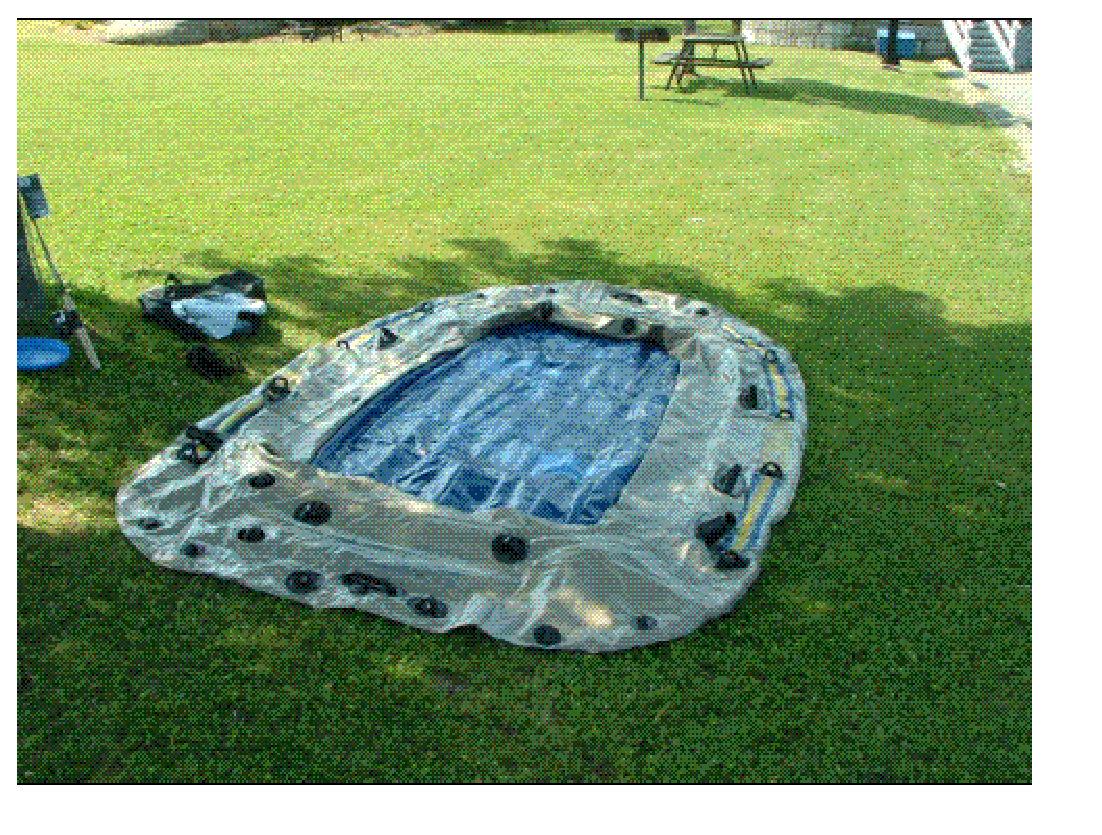
\epsfig{file=fig1.eps,width=3.5in}
Which one of the following is missing in it?
 
 
\noindent{\textbf{\large{
A.}}}
An air-boat
 
 
\noindent{\textbf{\large{
B.}}}
Lawn
 
 
\noindent{\textbf{\large{
C.}}}
A truck
 
 
\noindent{\textbf{\large{
D.}}}
An airplane
 
 
\noindent{\textbf{\large{
E.}}}
A table
 
 
\noindent{\textbf{\large{
F.}}}
  Not any of aboves.
 
 
\noindent\vspace{0.05in}{\textbf{\Large{Auto-answer:}}}
 
 
\noindent{\textbf{\large{
C.}}}
A truck
 
 
\noindent{\textbf{\large{
D.}}}
An airplane
 
 
\noindent\vspace{0.05in}{\textbf{\Large{End of auto-answer.}}}
 
 
 
\vspace{0.3in}
   
   
\noindent{\textbf{\Large{Total numbers: }}}
   
   
\noindent\begin{tabular}{|l|l|l|l|l|l|l|}
 \hline
Inputs & Calculates & Choices & Layers & Matches & Answer & Solution \\ \hline
           0 & 
           0 & 
           6
  simple  
  & 
           6 & 
           0 & 
  yes & 
  no 
  \\ \hline
 \end{tabular}
   
   
   
   
\noindent\vspace{0.1in}{\textbf{\Large{Calculated values:}}}
   
   
   
   
\noindent\vspace{0.1in}\hspace{-0.08in} {\textbf{\Large{All inputs: }}}
   
   
  
\vspace{0.2in}
  
{\textbf{\Large{Question
27.1.3 
 (          6,          6,         21)
}}}
  
  
 
An object is subjected to an external net force $\mathbf{f}=(
50.0,  % 
5.0,
-5000.0  )N$. Its mass is known as
$m= % 
50.0 kg$. Please calculate its accelaration.
 
 
 
 
\noindent\vspace{0.05in}{\textbf{\Large{Answer:}}}
 
 

We will use the Newton's Second Law:
 
\[
\mathbf{f}=m\mathbf{a}.
\]
 
Since $\mathbf{f}=( % 
50.0,  % 
5.0,  % 
-5000.0 )N$
and $m= % 
50.0 kg$, bring them into the above equation, then we get
 
\begin{eqnarray*}
\mathbf{a}&=&\frac{\mathbf{f}}m  \\
&=&\frac{(
50.0 ,
5.0 ,
-5000.0 )N
}{ % 
50.0 kg}  \\
&=&(
1.0000 ,
.10000,
-100.00
)ms^{-2} \\
&=&(
12960. ,
1296.0 ,
-1.2960 \times 10^{6}
)km/h^2.
\end{eqnarray*}
 
 
 
\noindent\vspace{0.05in}{\textbf{\Large{End of Answer.}}}
 
 

 
 
 
\noindent\vspace{0.1in}{\textbf{\Large{Solution: }}}
 
 

We will use the Newton's Second Law:
 
\[
\mathbf{f}=m\mathbf{a}.
\]
 
Since $\mathbf{f}=( % 
50.0,  % 
5.0,  % 
-5000.0 )N$
and $m= % 
50.0 kg$, bring them into the above equation, then we get
 
\begin{eqnarray*}
\mathbf{a}&=&\frac{\mathbf{f}}m  \\
&=&\frac{(
50.0 ,
5.0 ,
-5000.0 )N
}{ % 
50.0 kg}  \\
&=&(
1.0000 ,
.10000,
-100.00
)ms^{-2} \\
&=&(
12960. ,
1296.0 ,
-1.2960 \times 10^{6}
)km/h^2.
\end{eqnarray*}
 
 
 
\noindent\vspace{0.1in}{\textbf{\Large{End of Solution.}}}
 
 

 
\vspace{0.3in}
   
   
\noindent{\textbf{\Large{Total numbers: }}}
   
   
\noindent\begin{tabular}{|l|l|l|l|l|l|l|}
 \hline
Inputs & Calculates & Choices & Layers & Matches & Answer & Solution \\ \hline
           4 & 
           6 & 
           0
  & 
           0 & 
           0 & 
  yes & 
  yes 
  \\ \hline
 \end{tabular}
   
   
   
   
\noindent\vspace{0.1in}{\textbf{\Large{Calculated values:}}}
   
   
  
  
\noindent\begin{tabular}{|l|l|l|l|}
\hline
 Sequential & Type & Accuracy & Calculated \\ 
\hline
 
 
  Calculated $           1$ & real & $           5 $ & 
 $ 1.0000 $ 
 \\  \hline  
 
 
  Calculated $           2$ & real & $           5 $ & 
 $ .10000 $ 
 \\  \hline  
 
 
  Calculated $           3$ & real & $           5 $ & 
 $ -100.00 $ 
 \\  \hline  
 
 
  Calculated $           4$ & real & $           5 $ & 
 $ 12960. $ 
 \\  \hline  
 
 
  Calculated $           5$ & real & $           5 $ & 
 $ 1296.0 $ 
 \\  \hline  
 
 
  Calculated $           6$ & real & $           5 $ & 
 $ -1.2960 \times 10^{6} $ 
 \\  \hline  
 \end{tabular}
   
   
   
   
\noindent\vspace{0.1in}\hspace{-0.08in} {\textbf{\Large{All inputs: }}}
   
   
  
  
\noindent\begin{tabular}{|l|l|l|l|l|}
\hline
 Sequential & Type & Accuracy & Three inputs & Generated \\ 
\hline
 
 
  INPUT $           1$ & real & $          -1 $ & $
 20.0
  $ & \\
  & & &  $
 101.0
  $ & \\
  & & &  $
 10.0
 $ & $ 50.0 $ 
 \\  \hline  
 
 
  INPUT $           2$ & real & $          -1 $ & $
 2.0
  $ & \\
  & & &  $
 10.1
  $ & \\
  & & &  $
 1.0
 $ & $ 5.0 $ 
 \\  \hline  
 
 
  INPUT $           3$ & real & $          -1 $ & $
 -2000.0
  $ & \\
  & & &  $
 -10001.0
  $ & \\
  & & &  $
 -1000.0
 $ & $ -5000.0 $ 
 \\  \hline  
 \end{tabular}
   
   
  
  
\noindent\begin{tabular}{|l|l|l|l|l|}
\hline
 Sequential & Type & Accuracy & Three inputs & Generated \\ 
\hline
 
 
  INPUT $           4$ & real & $          -1 $ & $
 50.0
  $ & \\
  & & &  $
 60.1
  $ & \\
  & & &  $
 2.0
 $ & $ 50.0 $ 
 \\  \hline  
 \end{tabular}
   
   
  
\vspace{0.2in}
  
{\textbf{\Large{Question
27.1.4 
 (          6,         11,         26)
}}}
  
  
In a hotel, the possiblity of  % 
smoking customer is
$a =  % 
7.0 \times 10^{-2}$, and the possiblity of  % 
equal or above 30 years old customer is $ b =  % 
.8200$.
Please calculate the possiblity of  % 
 non-smoking and  % 
under 30 years old customer.
 
 
 
\noindent\vspace{0.1in}{\textbf{\Large{Solution: }}}
 
 

Since the possiblity of  % 
smoking customer is $ a =  % 
7.0 \times 10^{-2} $,
and the possiblity of  % 
equal or above 30 years old customer is $ b =  % 
.8200 $,
the possiblity of  % 
non-smoking customer is $ c = 1.0 - a = 1.0 -
7.0 \times 10^{-2}
=  % 
.930 $ and the possiblity of  % 
under 30 years old
customer is $ d = 1.0 - b = 1.0 -  % 
.8200 =  % 
.1800  $.
So the possibility of  % 
 non-smoking and  % 
under 30 years old
customer is $ c \times d =  % 
.167 $.
 
 
 
\noindent\vspace{0.1in}{\textbf{\Large{End of Solution.}}}
 
 

 
 
 
\noindent\vspace{0.05in}{\textbf{\Large{Answer:}}}
 
 

The possibility of  % 
 non-smoking and  % 
under 30 years old
customer is $ (1-a)(1-b) =  % 
.167 $.
 
 
\noindent\vspace{0.05in}{\textbf{\Large{End of Answer.}}}
 
 

 
\vspace{0.3in}
   
   
\noindent{\textbf{\Large{Total numbers: }}}
   
   
\noindent\begin{tabular}{|l|l|l|l|l|l|l|}
 \hline
Inputs & Calculates & Choices & Layers & Matches & Answer & Solution \\ \hline
           4 & 
           3 & 
           0
  & 
           0 & 
           0 & 
  yes & 
  yes 
  \\ \hline
 \end{tabular}
   
   
   
   
\noindent\vspace{0.1in}{\textbf{\Large{Calculated values:}}}
   
   
  
  
\noindent\begin{tabular}{|l|l|l|l|}
\hline
 Sequential & Type & Accuracy & Calculated \\ 
\hline
 
 
  Calculated $           1$ & real & $           3 $ & 
 $ .930 $ 
 \\  \hline  
 
 
  Calculated $           2$ & real & $           4 $ & 
 $ .1800 $ 
 \\  \hline  
 
 
  Calculated $           3$ & real & $           3 $ & 
 $ .167 $ 
 \\  \hline  
 \end{tabular}
   
   
   
   
\noindent\vspace{0.1in}\hspace{-0.08in} {\textbf{\Large{All inputs: }}}
   
   
  
  
\noindent\begin{tabular}{|l|l|l|l|l|}
\hline
 Sequential & Type & Accuracy & Three inputs & Generated \\ 
\hline
 
 
  INPUT $           1$ & logical & .TRUE. & 
 smoking & 
  $ <-- $ 
  \\
  & & .FALSE. & 
  non-smoking & 
 \\  \hline  
 
 
  INPUT $           2$ & real & $          -3 $ & $
 1.0 \times 10^{-2}
  $ & \\
  & & &  $
 1.000
  $ & \\
  & & &  $
 1.0 \times 10^{-2}
 $ & $ 7.0 \times 10^{-2} $ 
 \\  \hline  
 
 
  INPUT $           3$ & logical & .TRUE. & 
 equal or above 30 years old & 
  $ <-- $ 
  \\
  & & .FALSE. & 
  under 30 years old & 
 \\  \hline  
 \end{tabular}
   
   
  
  
\noindent\begin{tabular}{|l|l|l|l|l|}
\hline
 Sequential & Type & Accuracy & Three inputs & Generated \\ 
\hline
 
 
  INPUT $           4$ & real & $          -4 $ & $
 2.00 \times 10^{-2}
  $ & \\
  & & &  $
 1.0000
  $ & \\
  & & &  $
 2.00 \times 10^{-2}
 $ & $ .8200 $ 
 \\  \hline  
 \end{tabular}
   
   
  
\vspace{0.2in}
  
{\textbf{\Large{Question
27.1.5 
 (          6,         13,         28)
}}}
  
  
What is the operation between $a= % 
5$ and $b= % 
4$:
$a$  % 
$\times$ $b=?$ Please also calculate it.
 
 
\noindent\vspace{0.05in}{\textbf{\Large{Answer:}}}
 
 

5;
 
4;
 
The operation is  % 
MULTIPLICATION and the result is
$ % 
20.000$.
 
 
 
\noindent\vspace{0.05in}{\textbf{\Large{End of Answer.}}}
 
 

 
\vspace{0.3in}
   
   
\noindent{\textbf{\Large{Total numbers: }}}
   
   
\noindent\begin{tabular}{|l|l|l|l|l|l|l|}
 \hline
Inputs & Calculates & Choices & Layers & Matches & Answer & Solution \\ \hline
           3 & 
           2 & 
           0
  & 
           0 & 
           0 & 
  yes & 
  no 
  \\ \hline
 \end{tabular}
   
   
   
   
\noindent\vspace{0.1in}{\textbf{\Large{Calculated values:}}}
   
   
  
  
\noindent\begin{tabular}{|l|l|l|l|}
\hline
 Sequential & Type & Accuracy & Calculated \\ 
\hline
 
 
  Calculated $           1$ & string & $           3 $ ( $          4 $ strings)
 : 
 & MULTIPLICATION
 \\  \hline  
 
 
  Calculated $           2$ & real & $           5 $ & 
 $ 20.000 $ 
 \\  \hline  
 \end{tabular}
   
   
   
   
\noindent\vspace{0.1in}\hspace{-0.08in} {\textbf{\Large{All inputs: }}}
   
   
  
  
\noindent\begin{tabular}{|l|l|l|l|l|}
\hline
 Sequential & Type & Accuracy & Three inputs & Generated \\ 
\hline
 
 
  INPUT $           1$ & integer &  & $
 1
 , 
 10
 , 
 2
 $ & $ 5 $ 
 \\  \hline  
 
 
  INPUT $           2$ & integer &  & $
 2
 , 
 10
 , 
 2
 $ & $ 4 $ 
 \\  \hline  
 
 
  INPUT $           3$ & string & & 
 $+$ & 
  \\
  & & & 
 $-$ & 
  \\
  & & & 
 $\times$ & 
  $ <-- $ 
  \\
  & & & 
 $\div$ & 
 \\  \hline  
 \end{tabular}
   
   
  
\vspace{0.2in}
  
{\textbf{\Large{Question
27.1.6 
 (          6,          7,         22)
}}}
  
  
 
An object is subjected to an external net force $\mathbf{f}=(
30.0 ,
3.0,
-3000.0  )N$. Its mass is known as
$m= % 
52.0  kg$. Please choose the correct accelaration
from the following choices.
 
 
 
\noindent{\textbf{\large{
A.}}}
The accelaration (vector) is
$(
22208.,
747.69 ,
-2.6185 \times 10^{6}
)km/h^2.
$
 
 
\noindent{\textbf{\large{
B.}}}
The accelaration (vector) is
$(
-35808.,
747.69 ,
-1.7989 \times 10^{6}
)km/h^2.
$
 
 
\noindent{\textbf{\large{
C.}}}
The accelaration (vector) is
$(
-34372.,
747.69 ,
-2.6185 \times 10^{6}
)km/h^2.
$
 
 
\noindent{\textbf{\large{
D.}}}
The accelaration (vector) is
$(
-34372.,
747.69 ,
2.4415 \times 10^{6}
)km/h^2.
$
 
 
\noindent{\textbf{\large{
E.}}}
The accelaration (vector) is
$(
-34372.,
747.69 ,
-747692.
)km/h^2.
$
 
 
\noindent{\textbf{\large{
F.}}}
The accelaration (vector) is
$(
7476.9,
747.69 ,
-2.6185 \times 10^{6}
)km/h^2.
$
 
 
\noindent{\textbf{\large{
G.}}}
The accelaration (vector) is
$(
7476.9,
747.69 ,
2.4415 \times 10^{6}
)km/h^2.
$
 
 
\noindent{\textbf{\large{
H.}}}
The accelaration (vector) is
$(
-35808.,
747.69 ,
2.4415 \times 10^{6}
)km/h^2.
$
 
 
\noindent{\textbf{\large{
I.}}}
The accelaration (vector) is
$(
7476.9,
747.69 ,
-747692.
)km/h^2.
$
 
 
\noindent{\textbf{\large{
J.}}}
The accelaration (vector) is
$(
22208.,
747.69 ,
2.4415 \times 10^{6}
)km/h^2.
$
 
 
\noindent{\textbf{\large{
K.}}}
The accelaration (vector) is
$(
22208.,
747.69 ,
-1.7989 \times 10^{6}
)km/h^2.
$
 
 
\noindent{\textbf{\large{
L.}}}
The accelaration (vector) is
$(
-35808.,
747.69 ,
-747692.
)km/h^2.
$
 
 
\noindent\vspace{0.05in}{\textbf{\Large{Auto-answer:}}}
 
 
\noindent{\textbf{\large{
I.}}}
The accelaration (vector) is
$(
7476.9,
747.69 ,
-747692.
)km/h^2.
$
 
 
\noindent\vspace{0.05in}{\textbf{\Large{End of auto-answer.}}}
 
 
 
 
 
 
\noindent\vspace{0.1in}{\textbf{\Large{Solution: }}}
 
 

We will use the Newton's Second Law:
 
\[
\mathbf{f}=m\mathbf{a}.
\]
 
Since $\mathbf{f}=( % 
30.0,  % 
3.0,  % 
-3000.0 )N$
and $m= % 
52.0 kg$, bring them into the above equation, then we get
 
\begin{eqnarray*}
\mathbf{a}&=&\frac{\mathbf{f}}m  \\
&=&\frac{(
30.0 ,
3.0 ,
-3000.0 )N
}{ % 
52.0 kg}  \\
&=&(
.57692 ,
5.7692 \times 10^{-2},
-57.692
)ms^{-2} \\
&=&(
7476.9 ,
747.69 ,
-747692.
)km/h^2.
\end{eqnarray*}
 
 
 
\noindent\vspace{0.1in}{\textbf{\Large{End of Solution.}}}
 
 

 
 
\vspace{0.3in}
   
   
\noindent{\textbf{\Large{Total numbers: }}}
   
   
\noindent\begin{tabular}{|l|l|l|l|l|l|l|}
 \hline
Inputs & Calculates & Choices & Layers & Matches & Answer & Solution \\ \hline
           4 & 
           6 & 
          12
  & 
           2 & 
           0 & 
  yes & 
  yes 
  \\ \hline
 \end{tabular}
   
   
   
   
\noindent\vspace{0.1in}{\textbf{\Large{Calculated values:}}}
   
   
  
  
\noindent\begin{tabular}{|l|l|l|l|}
\hline
 Sequential & Type & Accuracy & Calculated \\ 
\hline
 
 
  Calculated $           1$ & real & $           5 $ & 
 $ .57692 $ 
 \\  \hline  
 
 
  Calculated $           2$ & real & $           5 $ & 
 $ 5.7692 \times 10^{-2} $ 
 \\  \hline  
 
 
  Calculated $           3$ & real & $           5 $ & 
 $ -57.692 $ 
 \\  \hline  
 
 
  Calculated $           4$ & real & $           5 $ & 
 $ 7476.9 $ 
 \\  \hline  
 
 
  Calculated $           5$ & real & $           5 $ & 
 $ 747.69 $ 
 \\  \hline  
 
 
  Calculated $           6$ & real & $           5 $ & 
 $ -747692. $ 
 \\  \hline  
 \end{tabular}
   
   
   
   
\noindent\vspace{0.1in}\hspace{-0.08in} {\textbf{\Large{All inputs: }}}
   
   
  
  
\noindent\begin{tabular}{|l|l|l|l|l|}
\hline
 Sequential & Type & Accuracy & Three inputs & Generated \\ 
\hline
 
 
  INPUT $           1$ & real & $          -1 $ & $
 20.0
  $ & \\
  & & &  $
 101.0
  $ & \\
  & & &  $
 10.0
 $ & $ 30.0 $ 
 \\  \hline  
 
 
  INPUT $           2$ & real & $          -1 $ & $
 2.0
  $ & \\
  & & &  $
 10.1
  $ & \\
  & & &  $
 1.0
 $ & $ 3.0 $ 
 \\  \hline  
 
 
  INPUT $           3$ & real & $          -1 $ & $
 -2000.0
  $ & \\
  & & &  $
 -10001.0
  $ & \\
  & & &  $
 -1000.0
 $ & $ -3000.0 $ 
 \\  \hline  
 \end{tabular}
   
   
  
  
\noindent\begin{tabular}{|l|l|l|l|l|}
\hline
 Sequential & Type & Accuracy & Three inputs & Generated \\ 
\hline
 
 
  INPUT $           4$ & real & $          -1 $ & $
 50.0
  $ & \\
  & & &  $
 60.1
  $ & \\
  & & &  $
 2.0
 $ & $ 52.0 $ 
 \\  \hline  
 \end{tabular}
   
   
   
   
\vspace{0.3in}
{\textbf{\LARGE{You have done all the above? A very good beginning, please go ahead.}}}
More constants the
Mass of electron
$m_e$$ =
9.109390 \times 10^{-31} $
kg
,
Universal gas constant
$R$$ =
8.315 $
J/(mol$\cdot $K)
,
$e$$ =
1.60217733 \times 10^{-19} $
C
, and
$m_p$$ =
1.6726231 \times 10^{-27} $
kg
%
may be very helpful.
\vspace{0.3in}
   
   
  
\vspace{0.2in}
  
{\textbf{\Large{QUESTION
27.2 
 (          4,          4,          4)
}}}
  
  
Considering case-insensitivity, please match the following same strings.
  
  
\begin{tabular}{|l|l|l|}
 \hline
 Column Left & Column Right  & Your choinces \\ 
 \hline
{\textbf{\large{
A.}}}
er
  & 
b
 & 
 \\ 
 \hline
{\textbf{\large{
B.}}}
 A= %
6/ %
2

  & 
ER
 & 
 \\ 
 \hline
{\textbf{\large{
C.}}}
B
  & 
YJH
 & 
 \\ 
 \hline
{\textbf{\large{
D.}}}
asdf(:)
  & 
 a= %
3
 & 
 \\ 
 \hline
{\textbf{\large{
E.}}}
yjh
  & 
ASDF(:)
 & 
 \\ 
 \hline
 \end{tabular}
  
  
 
 
\noindent\vspace{0.05in}{\textbf{\Large{Auto-answer:}}}
  
  
\begin{tabular}{|l|l|l|}
 \hline
 Column Left & Column Right  & Answers       \\ 
 \hline
{\textbf{\large{
A.}}}
er
  & 
b
 & 
{\textbf{\large{
C.}}}
 \\ 
 \hline
{\textbf{\large{
B.}}}
 A= %
6/ %
2

  & 
ER
 & 
{\textbf{\large{
A.}}}
 \\ 
 \hline
{\textbf{\large{
C.}}}
B
  & 
YJH
 & 
{\textbf{\large{
E.}}}
 \\ 
 \hline
{\textbf{\large{
D.}}}
asdf(:)
  & 
 a= %
3
 & 
{\textbf{\large{
B.}}}
 \\ 
 \hline
{\textbf{\large{
E.}}}
yjh
  & 
ASDF(:)
 & 
{\textbf{\large{
D.}}}
 \\ 
 \hline
 \end{tabular}
  
  
 
 
\noindent\vspace{0.05in}{\textbf{\Large{End of auto-answer.}}}
 
 
 
   
   
\noindent{\textbf{\Large{Total numbers: }}}
   
   
\noindent\begin{tabular}{|l|l|l|l|l|l|l|}
 \hline
Inputs & Calculates & Choices & Layers & Matches & Answer & Solution \\ \hline
           2 & 
           1 & 
           0
  & 
          16 & 
           5 & 
  yes & 
  no 
  \\ \hline
 \end{tabular}
   
   
   
   
\noindent\vspace{0.1in}{\textbf{\Large{Calculated values:}}}
   
   
  
  
\noindent\begin{tabular}{|l|l|l|l|}
\hline
 Sequential & Type & Accuracy & Calculated \\ 
\hline
 
 
  Calculated $           1$ & integer &  & 
  $ 3 $ 
 \\  \hline  
 \end{tabular}
   
   
   
   
\noindent\vspace{0.1in}\hspace{-0.08in} {\textbf{\Large{All inputs: }}}
   
   
  
  
\noindent\begin{tabular}{|l|l|l|l|l|}
\hline
 Sequential & Type & Accuracy & Three inputs & Generated \\ 
\hline
 
 
  INPUT $           1$ & integer &  & $
 2
 , 
 8
 , 
 2
 $ & $ 6 $ 
 \\  \hline  
 
 
  INPUT $           2$ & integer &  & $
 2
 , 
 3
 , 
 2
 $ & $ 2 $ 
 \\  \hline  
 \end{tabular}
   
   
  
\vspace{0.2in}
  
{\textbf{\Large{QUESTION
27.3 
 (          3,          3,          3)
}}}
  
  
Please choose the correct one from the following statements:
 
 
\noindent{\textbf{\large{
A.}}}
Canada has  %
10 provinces and  %
3 territories.
 
 
\noindent{\textbf{\large{
B.}}}
Canada has  %
37 provinces and  %
37 territories.
 
 
\noindent{\textbf{\large{
C.}}}
Canada has  %
36 provinces and  %
35 territories.
 
 
\noindent{\textbf{\large{
D.}}}
Canada has  %
35 provinces and  %
34 territories.
 
 
\noindent{\textbf{\large{
E.}}}
Canada has  %
33 provinces and  %
38 territories.
 
 
\noindent{\textbf{\large{
F.}}}
 None of above.
 
 
\noindent\vspace{0.05in}{\textbf{\Large{Auto-answer:}}}
 
 
\noindent{\textbf{\large{
A.}}}
Canada has  %
10 provinces and  %
3 territories.
 
 
\noindent\vspace{0.05in}{\textbf{\Large{End of auto-answer.}}}
 
 
   
   
\noindent{\textbf{\Large{Total numbers: }}}
   
   
\noindent\begin{tabular}{|l|l|l|l|l|l|l|}
 \hline
Inputs & Calculates & Choices & Layers & Matches & Answer & Solution \\ \hline
           0 & 
          20 & 
           6
  simple  
  & 
           6 & 
           0 & 
  yes & 
  no 
  \\ \hline
 \end{tabular}
   
   
   
   
\noindent\vspace{0.1in}{\textbf{\Large{Calculated values:}}}
   
   
  
  
\noindent\begin{tabular}{|l|l|l|l|}
\hline
 Sequential & Type & Accuracy & Calculated \\ 
\hline
 
 
  Calculated $           1$ & integer &  & 
  $ 10 $ 
 \\  \hline  
 
 
  Calculated $           2$ & integer &  & 
  $ 3 $ 
 \\  \hline  
 
 
  Calculated $           3$ & integer &  & 
  $ 23 $ 
 \\  \hline  
 
 
  Calculated $           4$ & integer &  & 
  $ 24 $ 
 \\  \hline  
 
 
  Calculated $           5$ & integer &  & 
  $ 25 $ 
 \\  \hline  
 
 
  Calculated $           6$ & integer &  & 
  $ 26 $ 
 \\  \hline  
 
 
  Calculated $           7$ & integer &  & 
  $ 27 $ 
 \\  \hline  
 
 
  Calculated $           8$ & integer &  & 
  $ 28 $ 
 \\  \hline  
 
 
  Calculated $           9$ & integer &  & 
  $ 29 $ 
 \\  \hline  
 
 
  Calculated $          10$ & integer &  & 
  $ 30 $ 
 \\  \hline  
 \end{tabular}
   
   
  
  
\noindent\begin{tabular}{|l|l|l|l|}
\hline
 Sequential & Type & Accuracy & Calculated \\ 
\hline
 
 
  Calculated $          11$ & integer &  & 
  $ 31 $ 
 \\  \hline  
 
 
  Calculated $          12$ & integer &  & 
  $ 32 $ 
 \\  \hline  
 
 
  Calculated $          13$ & integer &  & 
  $ 33 $ 
 \\  \hline  
 
 
  Calculated $          14$ & integer &  & 
  $ 34 $ 
 \\  \hline  
 
 
  Calculated $          15$ & integer &  & 
  $ 35 $ 
 \\  \hline  
 
 
  Calculated $          16$ & integer &  & 
  $ 36 $ 
 \\  \hline  
 
 
  Calculated $          17$ & integer &  & 
  $ 37 $ 
 \\  \hline  
 
 
  Calculated $          18$ & integer &  & 
  $ 38 $ 
 \\  \hline  
 
 
  Calculated $          19$ & integer &  & 
  $ 39 $ 
 \\  \hline  
 
 
  Calculated $          20$ & integer &  & 
  $ 40 $ 
 \\  \hline  
 \end{tabular}
   
   
   
   
\noindent\vspace{0.1in}\hspace{-0.08in} {\textbf{\Large{All inputs: }}}
   
   
  
\vspace{0.2in}
  
{\textbf{\Large{QUESTION
27.4 
 (          2,          2,          2)
}}}
  
  
 
An object is subjected to an external net force $\mathbf{f}=(
80.000 ,
9.0000,
-9000.0  )N$. Its mass is known as
$m= % 
58.0000  kg$. Please choose the correct accelaration
from the following choices.
 
 
 
\noindent{\textbf{\large{
A.}}}
The accelaration is
$(
-6.4083ms^{-2},
2011.0km/h^2,
-748.38ms^{-2}
).
$
 
 
\noindent{\textbf{\large{
B.}}}
The accelaration is
$(
-6.4083ms^{-2},
6610.6km/h^2,
-748.38ms^{-2}
).
$
 
 
\noindent{\textbf{\large{
C.}}}
The accelaration is
$(
1.3793ms^{-2},
2011.0km/h^2,
-748.38ms^{-2}
).
$
 
 
\noindent{\textbf{\large{
D.}}}
The accelaration is
$(
1.3793ms^{-2},
6610.6km/h^2,
-155.17ms^{-2}
).
$
 
 
\noindent{\textbf{\large{
E.}}}
The accelaration is
$(
1.3793ms^{-2},
2011.0km/h^2,
-155.17ms^{-2}
).
$
 
 
\noindent{\textbf{\large{
F.}}}
The accelaration is
$(
-6.4083ms^{-2},
6610.6km/h^2,
-155.17ms^{-2}
).
$
 
 
\noindent{\textbf{\large{
G.}}}
 None of these.
 
 
\noindent\vspace{0.05in}{\textbf{\Large{Auto-answer:}}}
 
 
\noindent{\textbf{\large{
E.}}}
The accelaration is
$(
1.3793ms^{-2},
2011.0km/h^2,
-155.17ms^{-2}
).
$
 
 
\noindent\vspace{0.05in}{\textbf{\Large{End of auto-answer.}}}
 
 
 
 
 
 
\noindent\vspace{0.1in}{\textbf{\Large{Solution: }}}
 
 

We will use the Newton's Second Law:
 
\[
\mathbf{f}=m\mathbf{a}.
\]
 
Since $\mathbf{f}=( % 
80.000,  % 
9.0000,  % 
-9000.0 )N$
and $m= % 
58.0000kg$, bring them into the above equation, then we get
 
\begin{eqnarray*}
\mathbf{a}&=&\frac{\mathbf{f}}m  \\
&=&\frac{(
80.000 ,
9.0000 ,
-9000.0 )N
}{ % 
58.0000 kg}  \\
&=&(
1.3793 ,
.15517,
-155.17
)ms^{-2} \\
&=&(
17876. ,
2011.0 ,
-2.0110 \times 10^{6}
)km/h^2.
\end{eqnarray*}
 
 
 
\noindent\vspace{0.1in}{\textbf{\Large{End of Solution.}}}
 
 

 
\vspace{0.3in}
   
   
\noindent{\textbf{\Large{Total numbers: }}}
   
   
\noindent\begin{tabular}{|l|l|l|l|l|l|l|}
 \hline
Inputs & Calculates & Choices & Layers & Matches & Answer & Solution \\ \hline
           4 & 
           6 & 
           7
  & 
           3 & 
           0 & 
  yes & 
  yes 
  \\ \hline
 \end{tabular}
   
   
   
   
\noindent\vspace{0.1in}{\textbf{\Large{Calculated values:}}}
   
   
  
  
\noindent\begin{tabular}{|l|l|l|l|}
\hline
 Sequential & Type & Accuracy & Calculated \\ 
\hline
 
 
  Calculated $           1$ & real & $           5 $ & 
 $ 1.3793 $ 
 \\  \hline  
 
 
  Calculated $           2$ & real & $           5 $ & 
 $ .15517 $ 
 \\  \hline  
 
 
  Calculated $           3$ & real & $           5 $ & 
 $ -155.17 $ 
 \\  \hline  
 
 
  Calculated $           4$ & real & $           5 $ & 
 $ 17876. $ 
 \\  \hline  
 
 
  Calculated $           5$ & real & $           5 $ & 
 $ 2011.0 $ 
 \\  \hline  
 
 
  Calculated $           6$ & real & $           5 $ & 
 $ -2.0110 \times 10^{6} $ 
 \\  \hline  
 \end{tabular}
   
   
   
   
\noindent\vspace{0.1in}\hspace{-0.08in} {\textbf{\Large{All inputs: }}}
   
   
  
  
\noindent\begin{tabular}{|l|l|l|l|l|}
\hline
 Sequential & Type & Accuracy & Three inputs & Generated \\ 
\hline
 
 
  INPUT $           1$ & real & $          -3 $ & $
 20.000
  $ & \\
  & & &  $
 101.000
  $ & \\
  & & &  $
 10.000
 $ & $ 80.000 $ 
 \\  \hline  
 
 
  INPUT $           2$ & real & $          -4 $ & $
 2.0000
  $ & \\
  & & &  $
 10.1000
  $ & \\
  & & &  $
 1.0000
 $ & $ 9.0000 $ 
 \\  \hline  
 
 
  INPUT $           3$ & real & $          -1 $ & $
 -2000.0
  $ & \\
  & & &  $
 -10001.0
  $ & \\
  & & &  $
 -1000.0
 $ & $ -9000.0 $ 
 \\  \hline  
 \end{tabular}
   
   
  
  
\noindent\begin{tabular}{|l|l|l|l|l|}
\hline
 Sequential & Type & Accuracy & Three inputs & Generated \\ 
\hline
 
 
  INPUT $           4$ & real & $          -4 $ & $
 50.0000
  $ & \\
  & & &  $
 60.1000
  $ & \\
  & & &  $
 2.0000
 $ & $ 58.0000 $ 
 \\  \hline  
 \end{tabular}
   
   
  
\vspace{0.2in}
  
{\textbf{\Large{QUESTION
27.5 
 (          1,          1,          1)
}}}
  
  


\noindent\vspace{0.05in}{\textbf{\Large{Abstract:}}}
This is a simple Newton's Second Law calculation multi-choice problem.  
\noindent\vspace{0.05in}{\textbf{\Large{end of abstract.}}}


 
 
An object is subjected to an external net force $\mathbf{f}=
(40.0 , 2.0 , -2000.0) N$.
Its mass is known as $m= % 
52.0000 kg$. Please choose the
correct accelaration from the following choices.
 
 
 
\noindent{\textbf{\large{
A.}}}
The accelaration is $  %
(
3.47,
3.8 \times 10^{-2},
-38.462)
ms^{-2} $.
 
 
\noindent{\textbf{\large{
B.}}}
The accelaration is $  %
(
3.47,
3.8 \times 10^{-2},
-159.40)
ms^{-2} $.
 
 
\noindent{\textbf{\large{
C.}}}
The accelaration is $  %
(
.769,
.12,
-38.462)
ms^{-2} $.
 
 
\noindent{\textbf{\large{
D.}}}
The accelaration is $  %
(
.769,
3.8 \times 10^{-2},
-38.462)
ms^{-2} $.
 
 
\noindent{\textbf{\large{
E.}}}
The accelaration is $  %
(
.769,
3.8 \times 10^{-2},
-159.40)
ms^{-2} $.
 
 
\noindent{\textbf{\large{
F.}}}
The accelaration is $  %
(
3.47,
.12,
-159.40)
ms^{-2} $.
 
 
\noindent{\textbf{\large{
G.}}}
The accelaration is $  %
(
3.47,
.12,
-38.462)
ms^{-2} $.
 
 
\noindent{\textbf{\large{
H.}}}
The accelaration is $  %
(
.769,
.12,
-159.40)
ms^{-2} $.
 
 
\noindent\vspace{0.05in}{\textbf{\Large{Auto-answer:}}}
 
 
\noindent{\textbf{\large{
D.}}}
The accelaration is $  %
(
.769,
3.8 \times 10^{-2},
-38.462)
ms^{-2} $.
 
 
\noindent\vspace{0.05in}{\textbf{\Large{End of auto-answer.}}}
 
 
 
 
 
\noindent\vspace{0.05in}{\textbf{\Large{Answer:}}}
 
 

The correct answer from the choices is


\noindent{\textbf{\large{
D.}}}
The accelaration is $  %
(
.769,
3.8 \times 10^{-2},
-38.462)
ms^{-2} $.
 
 
 
\noindent\vspace{0.05in}{\textbf{\Large{End of Answer.}}}
 
 

 
 
 
\noindent\vspace{0.1in}{\textbf{\Large{Solution: }}}
 
 

We will use the Newton's Second Law:
 
\[
\mathbf{f}=m\mathbf{a}.
\]
 
Since $\mathbf{f}= % 
(40.0 , 2.0 , -2000.0) N$
and $m= % 
52.0000kg$, bring them into the above equation, then we get
 
\begin{eqnarray*}
\mathbf{a}&=&\frac{\mathbf{f}}m  \\
&=&\frac{ % 
(40.0 , 2.0 , -2000.0) N}{ % 
52.0000kg}  \\
&=& % 
(.769 , 3.8 \times 10^{-2} , -38.462) ms^{-2}
\end{eqnarray*}
 
 
 
\noindent\vspace{0.1in}{\textbf{\Large{End of Solution.}}}
 
 

 
\vspace{0.3in}
   
   
\noindent{\textbf{\Large{Total numbers: }}}
   
   
\noindent\begin{tabular}{|l|l|l|l|l|l|l|}
 \hline
Inputs & Calculates & Choices & Layers & Matches & Answer & Solution \\ \hline
           2 & 
           1 & 
           8
  & 
           3 & 
           0 & 
  yes & 
  yes 
  \\ \hline
 \end{tabular}
   
   
   
   
\noindent\vspace{0.1in}{\textbf{\Large{Calculated values:}}}
   
   
  
  
\noindent\begin{tabular}{|l|l|l|l|}
\hline
 Sequential & Type & Accuracy & Calculated \\ 
\hline
 
 
  Calculated $           1$ & vector &  
  $           3 $ 
 &  $ .769 $ 
 \\    
  & & 
  $           2 $ 
 &  $ 3.8 \times 10^{-2} $ 
 \\    
  & & 
  $           5 $ 
 &  $ -38.462 $ 
 \\  \hline  
 \end{tabular}
   
   
   
   
\noindent\vspace{0.1in}\hspace{-0.08in} {\textbf{\Large{All inputs: }}}
   
   
  
  
\noindent\begin{tabular}{|l|l|l|l|l|}
\hline
 Sequential & Type & Accuracy & Three inputs & Generated \\ 
\hline
 
 
  INPUT $           1$ & vector & $          -1 $ & $
20.0
  $ & \\
  & & & $
101.0
  $ & \\
  & & & $
10.0
$ & $ 40.0 $ 
  \\
  & & $          -1 $ & $
2.0
  $ & \\
  & & & $
10.1
  $ & \\
  & & & $
1.0
$ & $ 2.0 $ 
  \\
  & & $          -1 $ & $
-2000.0
  $ & \\
  & & & $
-10001.0
  $ & \\
  & & & $
-1000.0
$ & $ -2000.0 $ 
 \\  \hline  
 
 
  INPUT $           2$ & real & $          -4 $ & $
 50.0000
  $ & \\
  & & &  $
 60.1000
  $ & \\
  & & &  $
 2.0000
 $ & $ 52.0000 $ 
 \\  \hline  
 \end{tabular}
   
   
  
\vspace{0.2in}
  
{\textbf{\Large{QUESTION
27.6 
 (          5,          5,          5)
}}}
  
  
If any one of the following statements is correct, please fill the box ahead of it with $T$ .
If wrong, fill with $F$.
 
\noindent\begin{tabular}{|l|l|}\hline Your&\hspace{.2in} \\ answer&\hspace{.2in} \\ \hline \end{tabular}
1. $ % 
47$ is an  % 
even number.
 
\noindent\begin{tabular}{|l|l|}\hline Your&\hspace{.2in} \\ answer&\hspace{.2in} \\ \hline \end{tabular}
2.  % 
Montreal is in  % 
Ontario province.
 
\noindent\begin{tabular}{|l|l|}\hline Your&\hspace{.2in} \\ answer&\hspace{.2in} \\ \hline \end{tabular}
3.  % 
$\mathbf{F}=m\mathbf{a}$ is a mathmatical form of
the Newton's Second Law.
 
 
 
\noindent\vspace{0.05in}{\textbf{\Large{Answer:}}}
 
 

 
\noindent\begin{tabular}{|l|l|}\hline The correct & \\
          answer &  % 
$F$ \\ \hline \end{tabular}
1. $ % 
47$ is an  % 
even number.
 
\noindent\begin{tabular}{|l|l|}\hline The correct & \\
          answer &  % 
$F$ \\ \hline \end{tabular}
2.  % 
Montreal is in  % 
Ontario province.
 
\noindent\begin{tabular}{|l|l|}\hline The correct & \\
          answer &  % 
$T$ \\ \hline \end{tabular}
3.  % 
$\mathbf{F}=m\mathbf{a}$ is a mathmatical form of  % 
the Newton's Second Law.
 
 
 
\noindent\vspace{0.05in}{\textbf{\Large{End of Answer.}}}
 
 

 
\vspace{0.3in}
   
   
\noindent{\textbf{\Large{Total numbers: }}}
   
   
\noindent\begin{tabular}{|l|l|l|l|l|l|l|}
 \hline
Inputs & Calculates & Choices & Layers & Matches & Answer & Solution \\ \hline
           6 & 
           3 & 
           0
  & 
           0 & 
           0 & 
  yes & 
  no 
  \\ \hline
 \end{tabular}
   
   
   
   
\noindent\vspace{0.1in}{\textbf{\Large{Calculated values:}}}
   
   
  
  
\noindent\begin{tabular}{|l|l|l|l|}
\hline
 Sequential & Type & Accuracy & Calculated \\ 
\hline
 
 
  Calculated $           1$ & string & $           2 $ ( $          2 $ strings)
 : 
 & $F$
 \\  \hline  
 
 
  Calculated $           2$ & string & $           2 $ ( $          2 $ strings)
 : 
 & $F$
 \\  \hline  
 
 
  Calculated $           3$ & string & $           1 $ ( $          2 $ strings)
 : 
 & $T$
 \\  \hline  
 \end{tabular}
   
   
   
   
\noindent\vspace{0.1in}\hspace{-0.08in} {\textbf{\Large{All inputs: }}}
   
   
  
  
\noindent\begin{tabular}{|l|l|l|l|l|}
\hline
 Sequential & Type & Accuracy & Three inputs & Generated \\ 
\hline
 
 
  INPUT $           1$ & integer &  & $
 1
 , 
 100
 , 
 1
 $ & $ 47 $ 
 \\  \hline  
 
 
  INPUT $           2$ & string & & 
 even & 
  $ <-- $ 
  \\
  & & & 
 odd & 
 \\  \hline  
 
 
  INPUT $           3$ & string & & 
 Toronto & 
  \\
  & & & 
 Kingston & 
  \\
  & & & 
 Montreal & 
  $ <-- $ 
  \\
  & & & 
 Hull & 
 \\  \hline  
 \end{tabular}
   
   
  
  
\noindent\begin{tabular}{|l|l|l|l|l|}
\hline
 Sequential & Type & Accuracy & Three inputs & Generated \\ 
\hline
 
 
  INPUT $           4$ & string & & 
 Ontario & 
  $ <-- $ 
  \\
  & & & 
 Quebec & 
 \\  \hline  
 
 
  INPUT $           5$ & string & & 
 $\mathbf{F}=m\mathbf{a}$ & 
  $ <-- $ 
  \\
  & & & 
 $\left| \mathbf{F}\right| =Gm_1m_2r^{-2}$ & 
 \\  \hline  
 
 
  INPUT $           6$ & string & & 
 the Newton's Second Law & 
  $ <-- $ 
  \\
  & & & 
 Newton's Law of Universal Gravitation & 
 \\  \hline  
 \end{tabular}
   
   
   
   
\vspace{0.3in}
{\textbf{\LARGE{You have done all the above? Excellent! Not much left, please continue.}}}
\vspace{0.3in}
   
   
  
\vspace{0.2in}
  
{\textbf{\Large{QUESTION
27.7 
 (          8,         15,         60)
}}}
  
  
 
$ \left( \begin{array}{ccccccccc}
           5 & 
           7 & 
           7 & 
           6 \\ 
           5 & 
           4 & 
           6 & 
           5 \\ 
           6 & 
           6 & 
           5 & 
           5
\end{array}\right) \times
\left( \begin{array}{c}
           2 \\ 
           2 \\ 
           2 \\ 
           2
\end{array}\right) $ =?
 
 
$  % 
 \left( \begin{array}
 {
 c
 c
 }
                    \zeta & 
 \Theta \\ 
                    \Xi & 
 \Theta \\ 
 \eta & 
 \gamma \\ 
 \rho & 
 \delta
 \end{array} \right)
 \left( \begin{array}
 {
 c
 }
 \beta \\ 
 \beta
 \end{array} \right)
$ =?
 
 
 
\noindent\vspace{0.05in}{\textbf{\Large{Answer:}}}
 
 

 
$\left( \begin{array}{ccccccccccccccc}
           5 & 
           7 & 
           7 & 
           6 \\ 
           5 & 
           4 & 
           6 & 
           5 \\ 
           6 & 
           6 & 
           5 & 
           5
\end{array}\right) \times
\left( \begin{array}{c}
           2 \\ 
           2 \\ 
           2 \\ 
           2
\end{array}\right)  =
\left( \begin{array}{c}
          50 \\ 
          40 \\ 
          44
\end{array}\right)  $
 
$  % 
 \left( \begin{array}
 {
 c
 c
 }
                    \zeta & 
 \Theta \\ 
                    \Xi & 
 \Theta \\ 
 \eta & 
 \gamma \\ 
 \rho & 
 \delta
 \end{array} \right)
 \left( \begin{array}
 {
 c
 }
 \beta \\ 
 \beta
 \end{array} \right)
=
  \left( \begin{array}
 {
 c
 }
                    \zeta \times  \beta   +  \Theta \times  \beta \\ 
                    \Xi \times  \beta   +  \Theta \times  \beta \\ 
 \eta \times  \beta   +  \gamma \times  \beta \\ 
 \rho \times  \beta   +  \delta \times  \beta
 \end{array} \right)
$
 
 
 
\noindent\vspace{0.05in}{\textbf{\Large{End of Answer.}}}
 
 

 
 
 
\noindent\vspace{0.1in}{\textbf{\Large{Solution: }}}
 
 

 
 
\noindent\vspace{0.1in}{\textbf{\Large{End of Solution.}}}
 
 

 
\vspace{0.3in}
   
   
\noindent{\textbf{\Large{Total numbers: }}}
   
   
\noindent\begin{tabular}{|l|l|l|l|l|l|l|}
 \hline
Inputs & Calculates & Choices & Layers & Matches & Answer & Solution \\ \hline
           4 & 
           2 & 
           0
  & 
           0 & 
           0 & 
  yes & 
  yes 
  \\ \hline
 \end{tabular}
   
   
   
   
\noindent\vspace{0.1in}{\textbf{\Large{Calculated values:}}}
   
   
  
  
\noindent\begin{tabular}{|l|l|l|l|}
\hline
 Sequential & Type & Accuracy & Calculated \\ 
\hline
 
 
  Calculated $           1$ & i-matrix &  & 
 (size:           3 by           1)
 \\  \hline  
 \end{tabular}
   
   
$\begin{array}{
 c
 }
          50 \\ 
          40 \\ 
          44
 \end{array}  $ 
  
  
\noindent\begin{tabular}{|l|l|l|l|}
\hline
 Sequential & Type & Accuracy & Calculated \\ 
\hline
 
 
  Calculated $           2$ & s-matrix & & 
 (size:           4 by           1)
 \\  \hline  
 \end{tabular}
   
   
 $   \left( \begin{array}
 {
 c
 }
                    \zeta \times  \beta   +  \Theta \times  \beta \\ 
                    \Xi \times  \beta   +  \Theta \times  \beta \\ 
 \eta \times  \beta   +  \gamma \times  \beta \\ 
 \rho \times  \beta   +  \delta \times  \beta
 \end{array} \right) $ 
   
   
\noindent\vspace{0.1in}\hspace{-0.08in} {\textbf{\Large{All inputs: }}}
   
   
  
  
\noindent\begin{tabular}{|l|l|l|l|l|}
\hline
 Sequential & Type & Accuracy & Three inputs & Generated \\ 
\hline
 
 
  INPUT $           1$ & i-matrix &  & $
 4
 , 
 7
 , 
 1
 $ & (size:           3 by           4)
 \\  \hline  
 \end{tabular}
   
   
 $\begin{array}{
 c
 c
 c
 c
 }
           5 & 
           7 & 
           7 & 
           6 \\ 
           5 & 
           4 & 
           6 & 
           5 \\ 
           6 & 
           6 & 
           5 & 
           5
\end{array}  $ 
  
  
\noindent\begin{tabular}{|l|l|l|l|l|}
\hline
 Sequential & Type & Accuracy & Three inputs & Generated \\ 
\hline
 
 
  INPUT $           2$ & i-matrix &  & $
 2
 , 
 2
 , 
 1
 $ & (size:           4 by           1)
 \\  \hline  
 \end{tabular}
   
   
 $\begin{array}{
 c
 }
           2 \\ 
           2 \\ 
           2 \\ 
           2
\end{array}  $ 
  
  
\noindent\begin{tabular}{|l|l|l|l|l|}
\hline
 Sequential & Type & Accuracy & Three inputs & Generated \\ 
\hline
 
 
  INPUT $           3$ & s-matrix & & 
 $  \alpha $ & 
  \\
  & & & 
 $  \beta $ & 
  \\
  & & & 
 $  \gamma $ & 
  \\
  & & & 
 $  \delta $ & 
  \\
  & & & 
 $  \epsilon $ & 
  \\
  & & & 
 $  \varepsilon $ & 
  \\
  & & & 
 $                     \zeta $ & 
  \\
  & & & 
 $  \eta $ & 
  \\
  & & & 
 $  \rho $ & 
  \\
  & & & 
 $  \sigma $ & 
  \\
  & & & 
 $  \Gamma $ & 
  \\
  & & & 
 $  \Delta $ & 
  \\
  & & & 
 $  \Theta $ & 
  \\
  & & & 
 $  \Lambda $ & 
  \\
  & & & 
 $                     \Xi $ & 
  \\
  & & & 
 $  \Upsilon $ & 
  \\
  & & & 
 $  \Phi $ & 
  \\
  & & & 
 $  \Psi $ & 
  \\
  & & & 
 $  \Omega $ & 
  (size:           4 by           2)
 \\  \hline  
 \end{tabular}
   
   
 $  \left( \begin{array}
 {
 c
 c
 }
                    \zeta & 
 \Theta \\ 
                    \Xi & 
 \Theta \\ 
 \eta & 
 \gamma \\ 
 \rho & 
 \delta
 \end{array} \right) $ 
  
  
\noindent\begin{tabular}{|l|l|l|l|l|}
\hline
 Sequential & Type & Accuracy & Three inputs & Generated \\ 
\hline
 
 
  INPUT $           4$ & s-matrix & & 
 $  \beta $ & 
  \\
  & & & 
 $  \gamma $ & 
  (size:           2 by           1)
 \\  \hline  
 \end{tabular}
   
   
 $  \left( \begin{array}
 {
 c
 }
 \beta \\ 
 \beta
 \end{array} \right) $ 
  
\vspace{0.2in}
  
{\textbf{\Large{QUESTION
27.8 
 (          7,         14,         50)
}}}
  
  
 
An object is subjected to an external net force $\mathbf{f}=
(80.0 , 8.0 , -8000.0) N$.
Its mass is known as $m= % 
58.0 kg$.
Please choose the correct accelaration from the following choices.
 
 
\noindent{\textbf{\large{
A.}}}
  The accelaration is $  %
(
3.41,
.14,
533.78)
ms^{-2} $.
 
 
\noindent{\textbf{\large{
B.}}}
  The accelaration is $  %
(
1.38,
.14,
-137.93)
ms^{-2} $.
 
 
\noindent{\textbf{\large{
C.}}}
  The accelaration is $  %
(
1.38,
.14,
533.78)
ms^{-2} $.
 
 
\noindent{\textbf{\large{
D.}}}
  The accelaration is $  %
(
1.38,
.57,
533.78)
ms^{-2} $.
 
 
\noindent\vspace{0.05in}{\textbf{\Large{Auto-answer:}}}
 
 
\noindent{\textbf{\large{
B.}}}
  The accelaration is $  %
(
1.38,
.14,
-137.93)
ms^{-2} $.
 
 
\noindent\vspace{0.05in}{\textbf{\Large{End of auto-answer.}}}
 
 
 
 
 
\noindent\vspace{0.1in}{\textbf{\Large{Solution: }}}
 
 

We will use the Newton's Second Law:
 
\[
\mathbf{f}=m\mathbf{a}.
\]
 
Since $\mathbf{f}= % 
(80.0 , 8.0 , -8000.0) N$
and $m= % 
58.0kg$, bring them into the above equation, then we get
 
\begin{eqnarray*}
\mathbf{a}&=&\frac{\mathbf{f}}m  \\
&=&\frac{ % 
(80.0 , 8.0 , -8000.0) N}{ % 
58.0kg}  \\
&=& % 
(1.38 , .14 , -137.93) ms^{-2}
\end{eqnarray*}
 
 
 
\noindent\vspace{0.1in}{\textbf{\Large{End of Solution.}}}
 
 

 
 
\vspace{0.3in}
   
   
\noindent{\textbf{\Large{Total numbers: }}}
   
   
\noindent\begin{tabular}{|l|l|l|l|l|l|l|}
 \hline
Inputs & Calculates & Choices & Layers & Matches & Answer & Solution \\ \hline
           2 & 
           1 & 
           4
  & 
           3 & 
           0 & 
  yes & 
  yes 
  \\ \hline
 \end{tabular}
   
   
   
   
\noindent\vspace{0.1in}{\textbf{\Large{Calculated values:}}}
   
   
  
  
\noindent\begin{tabular}{|l|l|l|l|}
\hline
 Sequential & Type & Accuracy & Calculated \\ 
\hline
 
 
  Calculated $           1$ & vector &  
  $           3 $ 
 &  $ 1.38 $ 
 \\    
  & & 
  $           2 $ 
 &  $ .14 $ 
 \\    
  & & 
  $           5 $ 
 &  $ -137.93 $ 
 \\  \hline  
 \end{tabular}
   
   
   
   
\noindent\vspace{0.1in}\hspace{-0.08in} {\textbf{\Large{All inputs: }}}
   
   
  
  
\noindent\begin{tabular}{|l|l|l|l|l|}
\hline
 Sequential & Type & Accuracy & Three inputs & Generated \\ 
\hline
 
 
  INPUT $           1$ & vector & $          -1 $ & $
20.0
  $ & \\
  & & & $
101.0
  $ & \\
  & & & $
10.0
$ & $ 80.0 $ 
  \\
  & & $          -1 $ & $
2.0
  $ & \\
  & & & $
10.1
  $ & \\
  & & & $
1.0
$ & $ 8.0 $ 
  \\
  & & $          -1 $ & $
-2000.0
  $ & \\
  & & & $
-10001.0
  $ & \\
  & & & $
-1000.0
$ & $ -8000.0 $ 
 \\  \hline  
 
 
  INPUT $           2$ & real & $          -1 $ & $
 50.0
  $ & \\
  & & &  $
 60.1
  $ & \\
  & & &  $
 2.0
 $ & $ 58.0 $ 
 \\  \hline  
 \end{tabular}
   
   
  
\vspace{0.2in}
  
{\textbf{\Large{QUESTION
27.9 
 (          9,         16,         70)
}}}
  
  


\noindent\vspace{0.05in}{\textbf{\Large{Abstract:}}}
Quadratic Equation constructed from the following first two random (input) integers as roots,  
which of course should not show in the exam papers.  
\noindent\vspace{0.05in}{\textbf{\Large{end of abstract.}}}


 
 
% First root
% Second root

 
Please solve the following equation:
\begin{eqnarray*}
9 \times x^2  % 
-108
                 \times x    % 
-2925 =0
\end{eqnarray*}
 
 
 
\noindent\vspace{0.05in}{\textbf{\Large{Answer:}}}
 
 

25,  % 
-13
 
 
 
\noindent\vspace{0.05in}{\textbf{\Large{End of Answer.}}}
 
 

 
 
 
\noindent\vspace{0.1in}{\textbf{\Large{Solution: }}}
 
 

Roots to the equation
\begin{eqnarray*}
9 \times x^2  % 
-108
                 \times x    % 
-2925 =0
\end{eqnarray*}
are  % 
25 and  % 
-13 .
 
Let us verity  % 
25 first:
$  % 
9 \times x^2  % 
-108
                 \times x    % 
-2925
  = % 
5625+( % 
-2700)+( % 
-2925)
  = % 
2925+( % 
-2925)
  = % 
0
$
 
Then verity  % 
-13:
$  % 
9 \times x^2  % 
-108
                 \times x    % 
-2925
  = % 
1521+( % 
1404)+( % 
-2925)
  = % 
2925+( % 
-2925)
  = % 
0
$
 
 
 
\noindent\vspace{0.1in}{\textbf{\Large{End of Solution.}}}
 
 

 
\vspace{0.3in}
   
   
\noindent{\textbf{\Large{Total numbers: }}}
   
   
\noindent\begin{tabular}{|l|l|l|l|l|l|l|}
 \hline
Inputs & Calculates & Choices & Layers & Matches & Answer & Solution \\ \hline
           3 & 
          13 & 
           0
  & 
           0 & 
           0 & 
  yes & 
  yes 
  \\ \hline
 \end{tabular}
   
   
   
   
\noindent\vspace{0.1in}{\textbf{\Large{Calculated values:}}}
   
   
  
  
\noindent\begin{tabular}{|l|l|l|l|}
\hline
 Sequential & Type & Accuracy & Calculated \\ 
\hline
 
 
  Calculated $           1$ & integer &  & 
  $ 9 $ 
 \\  \hline  
 
 
  Calculated $           2$ & string & $           2 $ ( $          2 $ strings)
 : 
 & 
 \\  \hline  
 
 
  Calculated $           3$ & integer &  & 
  $ -108 $ 
 \\  \hline  
 
 
  Calculated $           4$ & string & $           2 $ ( $          2 $ strings)
 : 
 & 
 \\  \hline  
 
 
  Calculated $           5$ & integer &  & 
  $ -2925 $ 
 \\  \hline  
 
 
  Calculated $           6$ & integer &  & 
  $ 5625 $ 
 \\  \hline  
 
 
  Calculated $           7$ & integer &  & 
  $ -2700 $ 
 \\  \hline  
 
 
  Calculated $           8$ & integer &  & 
  $ 2925 $ 
 \\  \hline  
 
 
  Calculated $           9$ & integer &  & 
  $ 0 $ 
 \\  \hline  
 
 
  Calculated $          10$ & integer &  & 
  $ 1521 $ 
 \\  \hline  
 \end{tabular}
   
   
  
  
\noindent\begin{tabular}{|l|l|l|l|}
\hline
 Sequential & Type & Accuracy & Calculated \\ 
\hline
 
 
  Calculated $          11$ & integer &  & 
  $ 1404 $ 
 \\  \hline  
 
 
  Calculated $          12$ & integer &  & 
  $ 2925 $ 
 \\  \hline  
 
 
  Calculated $          13$ & integer &  & 
  $ 0 $ 
 \\  \hline  
 \end{tabular}
   
   
   
   
\noindent\vspace{0.1in}\hspace{-0.08in} {\textbf{\Large{All inputs: }}}
   
   
  
  
\noindent\begin{tabular}{|l|l|l|l|l|}
\hline
 Sequential & Type & Accuracy & Three inputs & Generated \\ 
\hline
 
 
  INPUT $           1$ & integer &  & $
 -11
 , 
 30
 , 
 4
 $ & $ 25 $ 
 \\  \hline  
 
 
  INPUT $           2$ & integer &  & $
 -31
 , 
 60
 , 
 3
 $ & $ -13 $ 
 \\  \hline  
 
 
  INPUT $           3$ & integer &  & $
 -15
 , 
 15
 , 
 2
 $ & $ 9 $ 
 \\  \hline  
 \end{tabular}
   
   
   
   
   
   
 \vspace{0.2in}
Here are still some constants for use:
 
 
\noindent\begin{tabular}{|l|l|l|}
\hline
Constant & Symbol & Value \\
\hline
 
Mass of proton &
$m_p$ &
 $ 1.6726231 \times 10^{-27} $
kg \\
\hline
 
Boltzmann's constant &
$k$ &
 $ 1.381 \times 10^{-23} $
J/K \\
\hline
 
\end{tabular}
 
Thank you very much for answering these questions!
 
{\textbf{\large{Please be advised}}} that in this paper there are questions from
27.1 through
27.9.
And any one of them may contain more than one sub-question, thus the total number
of sub-questions here is around 14, of which
13 should be answered.
 
   
   
\vspace{2.0in} PAPER TAIL GENERATED.
   
   
   
   
\vspace{1.0in} 
{\textbf{\large{ *** END OF PAPER, THANKS *** }}} 
   
   
\hspace{1.0in} By: 
         239(         26,          34)
   
   
   
   
\newpage 
\setcounter{page}{ 
    28001 } 
   
   
\noindent{\textbf{\huge{THIS IS THE JOURNAL FOR}}}
   
   
 {\textbf{ \Large{ PAPER NUMBER          28 }}}
   
   
\vspace{0.2in}
   
   
\markboth{Journal NOT for examinees !!! {\today}}{Journal NOT for examinees !!! {\today}}
   
   
   
   
   
   
 \vspace{0.2in}
 
 
{\Huge  THIS IS AN EXAMPLE OF}
 
{\Huge  PERSONALIZED TESTS. }
 
If needed, please use the following constants.
 
 
 
\noindent\begin{tabular}{|l|l|l|}
\hline
Constant & Symbol & Value \\
\hline
Acceleration due to earth's gravity &
$g$ &
 $ 9.80 $
m/s$^2$ \\
\hline
Avogadro's number &
$N_A$ &
 $ 6.0221367 \times 10^{23} $
mol$^{-1}$ \\
\hline
Boltzmann's constant &
$k$ &
 $ 1.380658 \times 10^{-23} $
J/K \\
\hline
Coulomb's constant &
$k$ &
 $ 8.99 \times 10^{9} $
N$\cdot $m$^2$/C$^2$ \\
\hline
Electron charge magnitiude &
$e$ &
 $ 1.60217733 \times 10^{-19} $
C \\
\hline
Permeability of free space &
$\mu _0$ &
 $ 1.25663706 \times 10^{-6} $
T$\cdot $m/A \\
\hline
Permittivity of free space &
$\epsilon _0$ &
 $ 8.854187817 \times 10^{-12} $
C$^2$/(N$\cdot $m$^2$) \\
\hline
Pi &
$\pi$ &
 $ 3.14159265 $
$ $ \\
\hline
Planck's constant &
$h$ &
 $ 6.6260755 \times 10^{-34} $
J$\cdot $s \\
\hline
Mass of electron &
$m_e$ &
 $ 9.1093897 \times 10^{-31} $
kg \\
\hline
\end{tabular}
 
 
\noindent\begin{tabular}{|l|l|l|}
\hline
Constant & Symbol & Value \\
\hline
Mass of neutron &
$m_n$ &
 $ 1.6749286 \times 10^{-27} $
kg \\
\hline
Mass of proton &
$m_p$ &
 $ 1.6726231 \times 10^{-27} $
kg \\
\hline
Speed of light in vacuum &
$c$ &
 $ 299792458. $
m/s \\
\hline
Universal gravitational constant &
$G$ &
 $ 6.67259 \times 10^{-11} $
N$\cdot $m$^2$/kg$^2$ \\
\hline
Universal gas constant &
$R$ &
 $ 8.314510 $
J/(mol$\cdot $K) \\
\hline
\end{tabular}
 
 
{\textbf{\large{Please be advised}}} that in this paper there are questions from
28.1 through
28.9.
And any one of them may contain more than one sub-question, thus the total number
of sub-questions here is around 14, of which
13 should be answered.
 
\vspace{0.3in}
 
 
   
   
 PAPER TITLE GENERATED.
   
   
   
\vspace{0.2in}
   
In this paper, big questions will be generated in the following order: 
   
   
            1(          6)
 ,
            2(          5)
 ,
            3(          3)
 ,
            4(          4)
 ,
            5(          1)
 ,
            6(          2)
 ,
            7(          8)
 ,
            8(          7)
 ,
            9(          9)
 .
  
\vspace{0.2in}
  
{\textbf{\Large{QUESTION
28.1 
 (          6)
}}}
  
  
 
{\textbf{\Large{Please answer ONLY
5 of the following
6 questions (Questions
28.1.1 through
28.1.6). }}}
 
Here are still some constants for use in the following questions:
 
 
\noindent\begin{tabular}{|l|l|l|}
\hline
Constant & Symbol & Value \\
\hline
 
Boltzmann's constant &
$k$ &
 $ 1.381 \times 10^{-23} $
J/K \\
\hline
 
Avogadro's number &
$N_A$ &
 $ 6.022 \times 10^{23} $
mol$^{-1}$ \\
\hline
 
Mass of electron &
$m_e$ &
 $ 9.1093897 \times 10^{-31} $
kg \\
\hline
 
\end{tabular}
 
   
\vspace{0.2in}
   
 In this big question of CHOOSE structure,           6 questions will be generat
 ed: 
  
  
            1(         11,         26)
 ,
            2(          7,         22)
 ,
            3(         10,         25)
 ,
            4(          6,         21)
 ,
            5(         12,         27)
 ,
            6(          9,         24)
 .
  
\vspace{0.2in}
  
{\textbf{\Large{Question
28.1.1 
 (          6,         11,         26)
}}}
  
  
In a hotel, the possiblity of  % 
smoking customer is
$a =  % 
.580$, and the possiblity of  % 
 under 30 years old customer is $ b =  % 
.6200$.
Please calculate the possiblity of  % 
 non-smoking and  % 
equal or above 30 years old customer.
 
 
 
\noindent\vspace{0.1in}{\textbf{\Large{Solution: }}}
 
 

Since the possiblity of  % 
smoking customer is $ a =  % 
.580 $,
and the possiblity of  % 
 under 30 years old customer is $ b =  % 
.6200 $,
the possiblity of  % 
non-smoking customer is $ c = 1.0 - a = 1.0 -
.580
=  % 
.420 $ and the possiblity of  % 
equal or above 30 years old
customer is $ d = 1.0 - b = 1.0 -  % 
.6200 =  % 
.3800  $.
So the possibility of  % 
 non-smoking and  % 
equal or above 30 years old
customer is $ c \times d =  % 
.160 $.
 
 
 
\noindent\vspace{0.1in}{\textbf{\Large{End of Solution.}}}
 
 

 
 
 
\noindent\vspace{0.05in}{\textbf{\Large{Answer:}}}
 
 

The possibility of  % 
 non-smoking and  % 
equal or above 30 years old
customer is $ (1-a)(1-b) =  % 
.160 $.
 
 
\noindent\vspace{0.05in}{\textbf{\Large{End of Answer.}}}
 
 

 
\vspace{0.3in}
   
   
\noindent{\textbf{\Large{Total numbers: }}}
   
   
\noindent\begin{tabular}{|l|l|l|l|l|l|l|}
 \hline
Inputs & Calculates & Choices & Layers & Matches & Answer & Solution \\ \hline
           4 & 
           3 & 
           0
  & 
           0 & 
           0 & 
  yes & 
  yes 
  \\ \hline
 \end{tabular}
   
   
   
   
\noindent\vspace{0.1in}{\textbf{\Large{Calculated values:}}}
   
   
  
  
\noindent\begin{tabular}{|l|l|l|l|}
\hline
 Sequential & Type & Accuracy & Calculated \\ 
\hline
 
 
  Calculated $           1$ & real & $           3 $ & 
 $ .420 $ 
 \\  \hline  
 
 
  Calculated $           2$ & real & $           4 $ & 
 $ .3800 $ 
 \\  \hline  
 
 
  Calculated $           3$ & real & $           3 $ & 
 $ .160 $ 
 \\  \hline  
 \end{tabular}
   
   
   
   
\noindent\vspace{0.1in}\hspace{-0.08in} {\textbf{\Large{All inputs: }}}
   
   
  
  
\noindent\begin{tabular}{|l|l|l|l|l|}
\hline
 Sequential & Type & Accuracy & Three inputs & Generated \\ 
\hline
 
 
  INPUT $           1$ & logical & .TRUE. & 
 smoking & 
  $ <-- $ 
  \\
  & & .FALSE. & 
  non-smoking & 
 \\  \hline  
 
 
  INPUT $           2$ & real & $          -3 $ & $
 1.0 \times 10^{-2}
  $ & \\
  & & &  $
 1.000
  $ & \\
  & & &  $
 1.0 \times 10^{-2}
 $ & $ .580 $ 
 \\  \hline  
 
 
  INPUT $           3$ & logical & .TRUE. & 
 equal or above 30 years old & 
  \\
  & & .FALSE. & 
  under 30 years old & 
  $ <-- $ 
 \\  \hline  
 \end{tabular}
   
   
  
  
\noindent\begin{tabular}{|l|l|l|l|l|}
\hline
 Sequential & Type & Accuracy & Three inputs & Generated \\ 
\hline
 
 
  INPUT $           4$ & real & $          -4 $ & $
 2.00 \times 10^{-2}
  $ & \\
  & & &  $
 1.0000
  $ & \\
  & & &  $
 2.00 \times 10^{-2}
 $ & $ .6200 $ 
 \\  \hline  
 \end{tabular}
   
   
  
\vspace{0.2in}
  
{\textbf{\Large{Question
28.1.2 
 (          6,          7,         22)
}}}
  
  
 
An object is subjected to an external net force $\mathbf{f}=(
80.0 ,
4.0,
-6000.0  )N$. Its mass is known as
$m= % 
58.0  kg$. Please choose the correct accelaration
from the following choices.
 
 
 
\noindent{\textbf{\large{
A.}}}
The accelaration (vector) is
$(
-79300.,
893.79 ,
6.1195 \times 10^{6}
)km/h^2.
$
 
 
\noindent{\textbf{\large{
B.}}}
The accelaration (vector) is
$(
17876.,
893.79 ,
-6.0272 \times 10^{6}
)km/h^2.
$
 
 
\noindent{\textbf{\large{
C.}}}
The accelaration (vector) is
$(
17876.,
893.79 ,
-1.3407 \times 10^{6}
)km/h^2.
$
 
 
\noindent{\textbf{\large{
D.}}}
The accelaration (vector) is
$(
-59537.,
893.79 ,
5.9065 \times 10^{6}
)km/h^2.
$
 
 
\noindent{\textbf{\large{
E.}}}
The accelaration (vector) is
$(
-59537.,
893.79 ,
-1.3407 \times 10^{6}
)km/h^2.
$
 
 
\noindent{\textbf{\large{
F.}}}
The accelaration (vector) is
$(
-59537.,
893.79 ,
-6.0272 \times 10^{6}
)km/h^2.
$
 
 
\noindent{\textbf{\large{
G.}}}
The accelaration (vector) is
$(
36162.,
893.79 ,
5.9065 \times 10^{6}
)km/h^2.
$
 
 
\noindent{\textbf{\large{
H.}}}
The accelaration (vector) is
$(
17876.,
893.79 ,
6.1195 \times 10^{6}
)km/h^2.
$
 
 
\noindent{\textbf{\large{
I.}}}
The accelaration (vector) is
$(
-79300.,
893.79 ,
-6.0272 \times 10^{6}
)km/h^2.
$
 
 
\noindent{\textbf{\large{
J.}}}
The accelaration (vector) is
$(
36162.,
893.79 ,
-1.3407 \times 10^{6}
)km/h^2.
$
 
 
\noindent{\textbf{\large{
K.}}}
The accelaration (vector) is
$(
36162.,
893.79 ,
6.1195 \times 10^{6}
)km/h^2.
$
 
 
\noindent{\textbf{\large{
L.}}}
The accelaration (vector) is
$(
-79300.,
893.79 ,
5.9065 \times 10^{6}
)km/h^2.
$
 
 
\noindent\vspace{0.05in}{\textbf{\Large{Auto-answer:}}}
 
 
\noindent{\textbf{\large{
C.}}}
The accelaration (vector) is
$(
17876.,
893.79 ,
-1.3407 \times 10^{6}
)km/h^2.
$
 
 
\noindent\vspace{0.05in}{\textbf{\Large{End of auto-answer.}}}
 
 
 
 
 
 
\noindent\vspace{0.1in}{\textbf{\Large{Solution: }}}
 
 

We will use the Newton's Second Law:
 
\[
\mathbf{f}=m\mathbf{a}.
\]
 
Since $\mathbf{f}=( % 
80.0,  % 
4.0,  % 
-6000.0 )N$
and $m= % 
58.0 kg$, bring them into the above equation, then we get
 
\begin{eqnarray*}
\mathbf{a}&=&\frac{\mathbf{f}}m  \\
&=&\frac{(
80.0 ,
4.0 ,
-6000.0 )N
}{ % 
58.0 kg}  \\
&=&(
1.3793 ,
6.8966 \times 10^{-2},
-103.45
)ms^{-2} \\
&=&(
17876. ,
893.79 ,
-1.3407 \times 10^{6}
)km/h^2.
\end{eqnarray*}
 
 
 
\noindent\vspace{0.1in}{\textbf{\Large{End of Solution.}}}
 
 

 
 
\vspace{0.3in}
   
   
\noindent{\textbf{\Large{Total numbers: }}}
   
   
\noindent\begin{tabular}{|l|l|l|l|l|l|l|}
 \hline
Inputs & Calculates & Choices & Layers & Matches & Answer & Solution \\ \hline
           4 & 
           6 & 
          12
  & 
           2 & 
           0 & 
  yes & 
  yes 
  \\ \hline
 \end{tabular}
   
   
   
   
\noindent\vspace{0.1in}{\textbf{\Large{Calculated values:}}}
   
   
  
  
\noindent\begin{tabular}{|l|l|l|l|}
\hline
 Sequential & Type & Accuracy & Calculated \\ 
\hline
 
 
  Calculated $           1$ & real & $           5 $ & 
 $ 1.3793 $ 
 \\  \hline  
 
 
  Calculated $           2$ & real & $           5 $ & 
 $ 6.8966 \times 10^{-2} $ 
 \\  \hline  
 
 
  Calculated $           3$ & real & $           5 $ & 
 $ -103.45 $ 
 \\  \hline  
 
 
  Calculated $           4$ & real & $           5 $ & 
 $ 17876. $ 
 \\  \hline  
 
 
  Calculated $           5$ & real & $           5 $ & 
 $ 893.79 $ 
 \\  \hline  
 
 
  Calculated $           6$ & real & $           5 $ & 
 $ -1.3407 \times 10^{6} $ 
 \\  \hline  
 \end{tabular}
   
   
   
   
\noindent\vspace{0.1in}\hspace{-0.08in} {\textbf{\Large{All inputs: }}}
   
   
  
  
\noindent\begin{tabular}{|l|l|l|l|l|}
\hline
 Sequential & Type & Accuracy & Three inputs & Generated \\ 
\hline
 
 
  INPUT $           1$ & real & $          -1 $ & $
 20.0
  $ & \\
  & & &  $
 101.0
  $ & \\
  & & &  $
 10.0
 $ & $ 80.0 $ 
 \\  \hline  
 
 
  INPUT $           2$ & real & $          -1 $ & $
 2.0
  $ & \\
  & & &  $
 10.1
  $ & \\
  & & &  $
 1.0
 $ & $ 4.0 $ 
 \\  \hline  
 
 
  INPUT $           3$ & real & $          -1 $ & $
 -2000.0
  $ & \\
  & & &  $
 -10001.0
  $ & \\
  & & &  $
 -1000.0
 $ & $ -6000.0 $ 
 \\  \hline  
 \end{tabular}
   
   
  
  
\noindent\begin{tabular}{|l|l|l|l|l|}
\hline
 Sequential & Type & Accuracy & Three inputs & Generated \\ 
\hline
 
 
  INPUT $           4$ & real & $          -1 $ & $
 50.0
  $ & \\
  & & &  $
 60.1
  $ & \\
  & & &  $
 2.0
 $ & $ 58.0 $ 
 \\  \hline  
 \end{tabular}
   
   
  
\vspace{0.2in}
  
{\textbf{\Large{Question
28.1.3 
 (          6,         10,         25)
}}}
  
  
See the following picture.
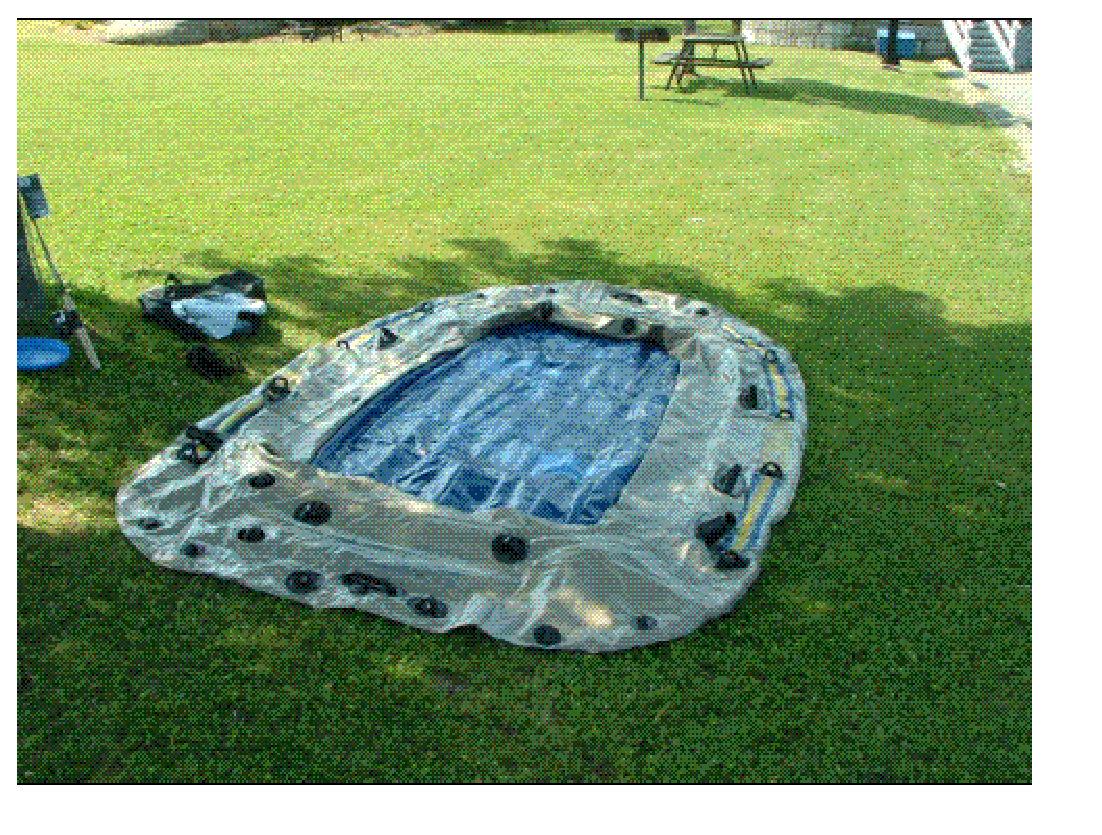
\epsfig{file=fig1.eps,width=3.5in}
Which one of the following is missing in it?
 
 
\noindent{\textbf{\large{
A.}}}
An air-boat
 
 
\noindent{\textbf{\large{
B.}}}
Lawn
 
 
\noindent{\textbf{\large{
C.}}}
An airplane
 
 
\noindent{\textbf{\large{
D.}}}
A truck
 
 
\noindent{\textbf{\large{
E.}}}
A table
 
 
\noindent{\textbf{\large{
F.}}}
  Not any of aboves.
 
 
\noindent\vspace{0.05in}{\textbf{\Large{Auto-answer:}}}
 
 
\noindent{\textbf{\large{
C.}}}
An airplane
 
 
\noindent{\textbf{\large{
D.}}}
A truck
 
 
\noindent\vspace{0.05in}{\textbf{\Large{End of auto-answer.}}}
 
 
 
\vspace{0.3in}
   
   
\noindent{\textbf{\Large{Total numbers: }}}
   
   
\noindent\begin{tabular}{|l|l|l|l|l|l|l|}
 \hline
Inputs & Calculates & Choices & Layers & Matches & Answer & Solution \\ \hline
           0 & 
           0 & 
           6
  simple  
  & 
           6 & 
           0 & 
  yes & 
  no 
  \\ \hline
 \end{tabular}
   
   
   
   
\noindent\vspace{0.1in}{\textbf{\Large{Calculated values:}}}
   
   
   
   
\noindent\vspace{0.1in}\hspace{-0.08in} {\textbf{\Large{All inputs: }}}
   
   
  
\vspace{0.2in}
  
{\textbf{\Large{Question
28.1.4 
 (          6,          6,         21)
}}}
  
  
 
An object is subjected to an external net force $\mathbf{f}=(
70.0,  % 
4.0,
-9000.0  )N$. Its mass is known as
$m= % 
56.0 kg$. Please calculate its accelaration.
 
 
 
 
\noindent\vspace{0.05in}{\textbf{\Large{Answer:}}}
 
 

We will use the Newton's Second Law:
 
\[
\mathbf{f}=m\mathbf{a}.
\]
 
Since $\mathbf{f}=( % 
70.0,  % 
4.0,  % 
-9000.0 )N$
and $m= % 
56.0 kg$, bring them into the above equation, then we get
 
\begin{eqnarray*}
\mathbf{a}&=&\frac{\mathbf{f}}m  \\
&=&\frac{(
70.0 ,
4.0 ,
-9000.0 )N
}{ % 
56.0 kg}  \\
&=&(
1.2500 ,
7.1429 \times 10^{-2},
-160.71
)ms^{-2} \\
&=&(
16200. ,
925.71 ,
-2.0829 \times 10^{6}
)km/h^2.
\end{eqnarray*}
 
 
 
\noindent\vspace{0.05in}{\textbf{\Large{End of Answer.}}}
 
 

 
 
 
\noindent\vspace{0.1in}{\textbf{\Large{Solution: }}}
 
 

We will use the Newton's Second Law:
 
\[
\mathbf{f}=m\mathbf{a}.
\]
 
Since $\mathbf{f}=( % 
70.0,  % 
4.0,  % 
-9000.0 )N$
and $m= % 
56.0 kg$, bring them into the above equation, then we get
 
\begin{eqnarray*}
\mathbf{a}&=&\frac{\mathbf{f}}m  \\
&=&\frac{(
70.0 ,
4.0 ,
-9000.0 )N
}{ % 
56.0 kg}  \\
&=&(
1.2500 ,
7.1429 \times 10^{-2},
-160.71
)ms^{-2} \\
&=&(
16200. ,
925.71 ,
-2.0829 \times 10^{6}
)km/h^2.
\end{eqnarray*}
 
 
 
\noindent\vspace{0.1in}{\textbf{\Large{End of Solution.}}}
 
 

 
\vspace{0.3in}
   
   
\noindent{\textbf{\Large{Total numbers: }}}
   
   
\noindent\begin{tabular}{|l|l|l|l|l|l|l|}
 \hline
Inputs & Calculates & Choices & Layers & Matches & Answer & Solution \\ \hline
           4 & 
           6 & 
           0
  & 
           0 & 
           0 & 
  yes & 
  yes 
  \\ \hline
 \end{tabular}
   
   
   
   
\noindent\vspace{0.1in}{\textbf{\Large{Calculated values:}}}
   
   
  
  
\noindent\begin{tabular}{|l|l|l|l|}
\hline
 Sequential & Type & Accuracy & Calculated \\ 
\hline
 
 
  Calculated $           1$ & real & $           5 $ & 
 $ 1.2500 $ 
 \\  \hline  
 
 
  Calculated $           2$ & real & $           5 $ & 
 $ 7.1429 \times 10^{-2} $ 
 \\  \hline  
 
 
  Calculated $           3$ & real & $           5 $ & 
 $ -160.71 $ 
 \\  \hline  
 
 
  Calculated $           4$ & real & $           5 $ & 
 $ 16200. $ 
 \\  \hline  
 
 
  Calculated $           5$ & real & $           5 $ & 
 $ 925.71 $ 
 \\  \hline  
 
 
  Calculated $           6$ & real & $           5 $ & 
 $ -2.0829 \times 10^{6} $ 
 \\  \hline  
 \end{tabular}
   
   
   
   
\noindent\vspace{0.1in}\hspace{-0.08in} {\textbf{\Large{All inputs: }}}
   
   
  
  
\noindent\begin{tabular}{|l|l|l|l|l|}
\hline
 Sequential & Type & Accuracy & Three inputs & Generated \\ 
\hline
 
 
  INPUT $           1$ & real & $          -1 $ & $
 20.0
  $ & \\
  & & &  $
 101.0
  $ & \\
  & & &  $
 10.0
 $ & $ 70.0 $ 
 \\  \hline  
 
 
  INPUT $           2$ & real & $          -1 $ & $
 2.0
  $ & \\
  & & &  $
 10.1
  $ & \\
  & & &  $
 1.0
 $ & $ 4.0 $ 
 \\  \hline  
 
 
  INPUT $           3$ & real & $          -1 $ & $
 -2000.0
  $ & \\
  & & &  $
 -10001.0
  $ & \\
  & & &  $
 -1000.0
 $ & $ -9000.0 $ 
 \\  \hline  
 \end{tabular}
   
   
  
  
\noindent\begin{tabular}{|l|l|l|l|l|}
\hline
 Sequential & Type & Accuracy & Three inputs & Generated \\ 
\hline
 
 
  INPUT $           4$ & real & $          -1 $ & $
 50.0
  $ & \\
  & & &  $
 60.1
  $ & \\
  & & &  $
 2.0
 $ & $ 56.0 $ 
 \\  \hline  
 \end{tabular}
   
   
  
\vspace{0.2in}
  
{\textbf{\Large{Question
28.1.5 
 (          6,         12,         27)
}}}
  
  
In a hotel, the possiblity of  % 
smoking customer is
$a =  % 
.120$, and the possiblity of  % 
equal-or-above 30 years old customer is $ b =  % 
.7000$.
Please fill the following form.
 
\noindent
\begin{tabular}{|l|l|}
\hline
Customer & Possibility \\
\hline
smoking  and   % 
equal-or-above 30 years old  & \\
\hline
smoking  and   % 
under 30 years old & \\
\hline
 non-smoking and   % 
equal-or-above 30 years old  & \\
\hline
 non-smoking and  % 
under 30 years old & \\
\hline
\end{tabular}
 
 
 
 
 
\noindent\vspace{0.1in}{\textbf{\Large{Solution: }}}
 
 

Since the possiblity of  % 
smoking customer is $ a =  % 
.120 $,
and the possiblity of  % 
equal-or-above 30 years old customer is $ b =  % 
.7000 $,
the possiblity of  % 
non-smoking customer is $ c = 1.0 - a = 1.0 -
.120
=  % 
.880 $ and the possiblity of  % 
under 30 years old
customer is $ d = 1.0 - b = 1.0 -  % 
.7000 =  % 
.3000  $.
Then
 
\noindent
\begin{tabular}{|l|l|}
\hline
Customer & Possibility \\
\hline
smoking  and  % 
equal-or-above 30 years old  &
  $ % 
.120 \times  % 
.7000 =  % 
8.40 \times 10^{-2}$ \\
\hline
smoking  and  % 
under 30 years old &
  $ % 
.120 \times  % 
.3000 =  % 
3.60 \times 10^{-2}$ \\
\hline
 non-smoking and  % 
equal-or-above 30 years old  &
  $ % 
.880 \times  % 
.7000 =  % 
.616$ \\
\hline
 non-smoking and  % 
under 30 years old &
  $ % 
.880 \times  % 
.3000 =  % 
.264$ \\
\hline
\end{tabular}
 
\noindent
And the total summation of all possibilities is $  % 
1.000 $.
 
 
 
 
\noindent\vspace{0.1in}{\textbf{\Large{End of Solution.}}}
 
 

 
 
 
\noindent\vspace{0.05in}{\textbf{\Large{Answer:}}}
 
 

 
\noindent
\begin{tabular}{|l|l|}
\hline
Customer & Possibility \\
\hline
smoking  and  % 
equal-or-above 30 years old &
  $ % 
8.40 \times 10^{-2}$ \\
\hline
smoking  and  % 
under 30 years old &
  $ % 
3.60 \times 10^{-2}$ \\
\hline
 non-smoking and  % 
equal-or-above 30 years old &
  $ % 
.616$ \\
\hline
 non-smoking and  % 
under 30 years old &
  $ % 
.264$ \\
\hline
\end{tabular}
 
\noindent
 And the total summation of all possibilities is $  % 
1.000 $.
 
 
 
\noindent\vspace{0.05in}{\textbf{\Large{End of Answer.}}}
 
 

 
\vspace{0.3in}
   
   
\noindent{\textbf{\Large{Total numbers: }}}
   
   
\noindent\begin{tabular}{|l|l|l|l|l|l|l|}
 \hline
Inputs & Calculates & Choices & Layers & Matches & Answer & Solution \\ \hline
           4 & 
          11 & 
           0
  & 
           0 & 
           0 & 
  yes & 
  yes 
  \\ \hline
 \end{tabular}
   
   
   
   
\noindent\vspace{0.1in}{\textbf{\Large{Calculated values:}}}
   
   
  
  
\noindent\begin{tabular}{|l|l|l|l|}
\hline
 Sequential & Type & Accuracy & Calculated \\ 
\hline
 
 
  Calculated $           1$ & real & $           3 $ & 
 $ .880 $ 
 \\  \hline  
 
 
  Calculated $           2$ & real & $           4 $ & 
 $ .3000 $ 
 \\  \hline  
 
 
  Calculated $           3$ & real & $           3 $ & 
 $ .120 $ 
 \\  \hline  
 
 
  Calculated $           4$ & real & $           3 $ & 
 $ .880 $ 
 \\  \hline  
 
 
  Calculated $           5$ & real & $           4 $ & 
 $ .7000 $ 
 \\  \hline  
 
 
  Calculated $           6$ & real & $           4 $ & 
 $ .3000 $ 
 \\  \hline  
 
 
  Calculated $           7$ & real & $           3 $ & 
 $ 8.40 \times 10^{-2} $ 
 \\  \hline  
 
 
  Calculated $           8$ & real & $           3 $ & 
 $ 3.60 \times 10^{-2} $ 
 \\  \hline  
 
 
  Calculated $           9$ & real & $           3 $ & 
 $ .616 $ 
 \\  \hline  
 
 
  Calculated $          10$ & real & $           3 $ & 
 $ .264 $ 
 \\  \hline  
 \end{tabular}
   
   
  
  
\noindent\begin{tabular}{|l|l|l|l|}
\hline
 Sequential & Type & Accuracy & Calculated \\ 
\hline
 
 
  Calculated $          11$ & real & $           4 $ & 
 $ 1.000 $ 
 \\  \hline  
 \end{tabular}
   
   
   
   
\noindent\vspace{0.1in}\hspace{-0.08in} {\textbf{\Large{All inputs: }}}
   
   
  
  
\noindent\begin{tabular}{|l|l|l|l|l|}
\hline
 Sequential & Type & Accuracy & Three inputs & Generated \\ 
\hline
 
 
  INPUT $           1$ & logical & .TRUE. & 
 smoking & 
  $ <-- $ 
  \\
  & & .FALSE. & 
  non-smoking & 
 \\  \hline  
 
 
  INPUT $           2$ & real & $          -3 $ & $
 1.0 \times 10^{-2}
  $ & \\
  & & &  $
 1.000
  $ & \\
  & & &  $
 1.0 \times 10^{-2}
 $ & $ .120 $ 
 \\  \hline  
 
 
  INPUT $           3$ & logical & .TRUE. & 
 equal-or-above 30 years old & 
  $ <-- $ 
  \\
  & & .FALSE. & 
  under 30 years old & 
 \\  \hline  
 \end{tabular}
   
   
  
  
\noindent\begin{tabular}{|l|l|l|l|l|}
\hline
 Sequential & Type & Accuracy & Three inputs & Generated \\ 
\hline
 
 
  INPUT $           4$ & real & $          -4 $ & $
 2.00 \times 10^{-2}
  $ & \\
  & & &  $
 1.0000
  $ & \\
  & & &  $
 2.00 \times 10^{-2}
 $ & $ .7000 $ 
 \\  \hline  
 \end{tabular}
   
   
  
\vspace{0.2in}
  
{\textbf{\Large{Question
28.1.6 
 (          6,          9,         24)
}}}
  
  
Let us use Newton's Law of Universal Gravitation to calculate the force
of the Sun acting on the eight planets. Let us suppose the mass of the
Sun is $ % 
9.00 \times 10^{24} kg$. With the mass and the
distance to the Sun of each planet in the following table, please fill
the blanks for the forces.
 
\vspace{0.2in}
 
 
\begin{tabular}{|l|l|l|l|}
\hline
The Planet & Mass ($kg$) & Distanace from Sun ($m$) & The Force ($N$)\\
\hline
Mercury  &
           $ % 
5.00000000 \times 10^{24} $   &
             $ % 
2.000000000 \times 10^{24} $    &
\\  \hline
Venus    &
           $ % 
6.00 \times 10^{24} $    &
             $ % 
4.00 \times 10^{24} $    &
\\  \hline
Earth    &
           $ % 
7.00 \times 10^{24} $    &
             $ % 
5.00 \times 10^{24} $    &
\\   \hline
Mars     &
           $ % 
7.00 \times 10^{24} $    &
             $ % 
7.00 \times 10^{24} $    &
\\   \hline
Jupiter  &
           $ % 
5.00 \times 10^{24} $    &
             $ % 
3.00 \times 10^{24} $    &
\\  \hline
Saturn   &
           $ % 
7.00 \times 10^{24}$    &
             $ % 
6.00 \times 10^{24}$    &
\\  \hline
Uranus   &
           $ % 
9.00 \times 10^{24} $    &
             $ % 
6.00 \times 10^{24} $    &
\\  \hline
Neptune  &
           $ % 
5.00 \times 10^{24} $    &
             $ % 
7.00 \times 10^{24} $    &
\\  \hline
 
\end{tabular}
 
 
 
 
\noindent\vspace{0.1in}{\textbf{\Large{Solution: }}}
 
 

By using Newton's Law of Universal Gravitation:
\[
F=G \frac{(Sun's \hspace{0.1in} mass) \times (Planet's \hspace{0.1in} mass)} { (distance)^2},
\]
where
$ G= % 
6.67 \times 10^{-11}N m^{2}(kg)^{-2}$ , the forces can be easily calculated as
 
\vspace{0.2in}
 
 
\begin{tabular}{|l|l|l|l|}
\hline
The Planet & Mass ($kg$) & Distanace from Sun ($m$) & The Force ($N$)\\
\hline
Mercury  &
           $ % 
5.00000000 \times 10^{24} $   &
             $ % 
2.000000000 \times 10^{24} $    & $ % 
7.50 \times 10^{-10} $
\\  \hline
Venus    &
           $  % 
6.00 \times 10^{24}  $     &
             $ % 
4.00 \times 10^{24} $    & $ % 
2.25 \times 10^{-10} $
\\  \hline
Earth    &
           $  % 
7.00 \times 10^{24}  $     &
             $ % 
5.00 \times 10^{24} $    & $ % 
1.68 \times 10^{-10} $
\\   \hline
Mars     &
           $  % 
7.00 \times 10^{24} $     &
             $ % 
7.00 \times 10^{24} $    & $ % 
8.58 \times 10^{-11} $
\\   \hline
Jupiter  &
           $  % 
5.00 \times 10^{24} $    &
             $ % 
3.00 \times 10^{24} $    & $ % 
3.33 \times 10^{-10} $
\\  \hline
Saturn   &
           $  % 
7.00 \times 10^{24} $    &
             $ % 
6.00 \times 10^{24}  $    & $ % 
1.17 \times 10^{-10} $
\\  \hline
Uranus   &
           $  % 
9.00 \times 10^{24} $    &
             $ % 
6.00 \times 10^{24} $    & $ % 
1.50 \times 10^{-10} $
\\  \hline
Neptune  &
           $  % 
5.00 \times 10^{24} $    &
             $ % 
7.00 \times 10^{24} $    & $ % 
6.13 \times 10^{-11} $
\\  \hline
 
\end{tabular}
 
 
 
 
\noindent\vspace{0.1in}{\textbf{\Large{End of Solution.}}}
 
 

 
 
 
 
\noindent\vspace{0.05in}{\textbf{\Large{Answer:}}}
 
 

By using Newton's Law of Universal Gravitation:
\[
F=G \frac{(Sun's \hspace{0.1in} mass) \times (Planet's \hspace{0.1in} mass)} { (distance)^2},
\]
where
$ G= % 
6.67 \times 10^{-11} N m^{2}(kg)^{-2}$ , the forces can be easily calculated as
 
\vspace{0.2in}
 
 
\begin{tabular}{|l|l|l|l|}
\hline
The Planet & Mass ($kg$) & Distanace from Sun ($m$) & The Force ($N$)\\
\hline
Mercury  &
           $ % 
5.00000000 \times 10^{24}  $   &
             $ % 
2.000000000 \times 10^{24}$    & $ % 
7.50 \times 10^{-10} $
\\  \hline
Venus    &
           $  % 
6.00 \times 10^{24}  $     &
             $ % 
4.00 \times 10^{24} $    & $ % 
2.25 \times 10^{-10} $
\\  \hline
Earth    &
           $  % 
7.00 \times 10^{24}$     &
             $ % 
5.00 \times 10^{24} $    & $ % 
1.68 \times 10^{-10} $
\\   \hline
Mars     &
           $  % 
7.00 \times 10^{24} $     &
             $ % 
7.00 \times 10^{24}$    & $ % 
8.58 \times 10^{-11} $
\\   \hline
Jupiter  &
           $  % 
5.00 \times 10^{24}  $    &
             $ % 
3.00 \times 10^{24} $    & $ % 
3.33 \times 10^{-10}3 $
\\  \hline
Saturn   &
           $  % 
7.00 \times 10^{24}   $    &
             $ % 
6.00 \times 10^{24}  $    & $ % 
1.17 \times 10^{-10} $
\\  \hline
Uranus   &
           $  % 
9.00 \times 10^{24} $    &
             $ % 
6.00 \times 10^{24}$    & $ % 
1.50 \times 10^{-10} $
\\  \hline
Neptune  &
           $  % 
5.00 \times 10^{24}  $    &
             $ % 
7.00 \times 10^{24} $    & $ % 
6.13 \times 10^{-11} $
\\  \hline
 
\end{tabular}
 
 
 
 
\noindent\vspace{0.05in}{\textbf{\Large{End of Answer.}}}
 
 

 
\vspace{0.3in}
   
   
\noindent{\textbf{\Large{Total numbers: }}}
   
   
\noindent\begin{tabular}{|l|l|l|l|l|l|l|}
 \hline
Inputs & Calculates & Choices & Layers & Matches & Answer & Solution \\ \hline
          19 & 
           8 & 
           0
  & 
           0 & 
           0 & 
  yes & 
  yes 
  \\ \hline
 \end{tabular}
   
   
   
   
\noindent\vspace{0.1in}{\textbf{\Large{Calculated values:}}}
   
   
  
  
\noindent\begin{tabular}{|l|l|l|l|}
\hline
 Sequential & Type & Accuracy & Calculated \\ 
\hline
 
 
  Calculated $           1$ & real & $           3 $ & 
 $ 7.50 \times 10^{-10} $ 
 \\  \hline  
 
 
  Calculated $           2$ & real & $           3 $ & 
 $ 2.25 \times 10^{-10} $ 
 \\  \hline  
 
 
  Calculated $           3$ & real & $           3 $ & 
 $ 1.68 \times 10^{-10} $ 
 \\  \hline  
 
 
  Calculated $           4$ & real & $           3 $ & 
 $ 8.58 \times 10^{-11} $ 
 \\  \hline  
 
 
  Calculated $           5$ & real & $           3 $ & 
 $ 3.33 \times 10^{-10} $ 
 \\  \hline  
 
 
  Calculated $           6$ & real & $           3 $ & 
 $ 1.17 \times 10^{-10} $ 
 \\  \hline  
 
 
  Calculated $           7$ & real & $           3 $ & 
 $ 1.50 \times 10^{-10} $ 
 \\  \hline  
 
 
  Calculated $           8$ & real & $           3 $ & 
 $ 6.13 \times 10^{-11} $ 
 \\  \hline  
 \end{tabular}
   
   
   
   
\noindent\vspace{0.1in}\hspace{-0.08in} {\textbf{\Large{All inputs: }}}
   
   
  
  
\noindent\begin{tabular}{|l|l|l|l|l|}
\hline
 Sequential & Type & Accuracy & Three inputs & Generated \\ 
\hline
 
 
  INPUT $           1$ & real & $          22 $ & $
 2.00 \times 10^{24}
  $ & \\
  & & &  $
 1.010 \times 10^{25}
  $ & \\
  & & &  $
 10.0 \times 10^{23}
 $ & $ 9.00 \times 10^{24} $ 
 \\  \hline  
 
 
  INPUT $           2$ & real & $          16 $ & $
 2.00000000 \times 10^{24}
  $ & \\
  & & &  $
 1.010000000 \times 10^{25}
  $ & \\
  & & &  $
 10.0000000 \times 10^{23}
 $ & $ 5.00000000 \times 10^{24} $ 
 \\  \hline  
 
 
  INPUT $           3$ & real & $          15 $ & $
 2.000000000 \times 10^{24}
  $ & \\
  & & &  $
 1.0100000000 \times 10^{25}
  $ & \\
  & & &  $
 10.00000000 \times 10^{23}
 $ & $ 2.000000000 \times 10^{24} $ 
 \\  \hline  
 \end{tabular}
   
   
  
  
\noindent\begin{tabular}{|l|l|l|l|l|}
\hline
 Sequential & Type & Accuracy & Three inputs & Generated \\ 
\hline
 
 
  INPUT $           4$ & real & $          22 $ & $
 2.00 \times 10^{24}
  $ & \\
  & & &  $
 1.010 \times 10^{25}
  $ & \\
  & & &  $
 10.0 \times 10^{23}
 $ & $ 6.00 \times 10^{24} $ 
 \\  \hline  
 
 
  INPUT $           5$ & real & $          22 $ & $
 2.00 \times 10^{24}
  $ & \\
  & & &  $
 1.010 \times 10^{25}
  $ & \\
  & & &  $
 10.0 \times 10^{23}
 $ & $ 4.00 \times 10^{24} $ 
 \\  \hline  
 
 
  INPUT $           6$ & real & $          22 $ & $
 2.00 \times 10^{24}
  $ & \\
  & & &  $
 1.010 \times 10^{25}
  $ & \\
  & & &  $
 10.0 \times 10^{23}
 $ & $ 7.00 \times 10^{24} $ 
 \\  \hline  
 \end{tabular}
   
   
  
  
\noindent\begin{tabular}{|l|l|l|l|l|}
\hline
 Sequential & Type & Accuracy & Three inputs & Generated \\ 
\hline
 
 
  INPUT $           7$ & real & $          22 $ & $
 2.00 \times 10^{24}
  $ & \\
  & & &  $
 1.010 \times 10^{25}
  $ & \\
  & & &  $
 10.0 \times 10^{23}
 $ & $ 5.00 \times 10^{24} $ 
 \\  \hline  
 
 
  INPUT $           8$ & real & $          22 $ & $
 2.00 \times 10^{24}
  $ & \\
  & & &  $
 1.010 \times 10^{25}
  $ & \\
  & & &  $
 10.0 \times 10^{23}
 $ & $ 7.00 \times 10^{24} $ 
 \\  \hline  
 
 
  INPUT $           9$ & real & $          22 $ & $
 2.00 \times 10^{24}
  $ & \\
  & & &  $
 1.010 \times 10^{25}
  $ & \\
  & & &  $
 10.0 \times 10^{23}
 $ & $ 7.00 \times 10^{24} $ 
 \\  \hline  
 \end{tabular}
   
   
  
  
\noindent\begin{tabular}{|l|l|l|l|l|}
\hline
 Sequential & Type & Accuracy & Three inputs & Generated \\ 
\hline
 
 
  INPUT $          10$ & real & $          22 $ & $
 2.00 \times 10^{24}
  $ & \\
  & & &  $
 1.010 \times 10^{25}
  $ & \\
  & & &  $
 10.0 \times 10^{23}
 $ & $ 5.00 \times 10^{24} $ 
 \\  \hline  
 
 
  INPUT $          11$ & real & $          22 $ & $
 2.00 \times 10^{24}
  $ & \\
  & & &  $
 1.010 \times 10^{25}
  $ & \\
  & & &  $
 10.0 \times 10^{23}
 $ & $ 3.00 \times 10^{24} $ 
 \\  \hline  
 
 
  INPUT $          12$ & real & $          22 $ & $
 2.00 \times 10^{24}
  $ & \\
  & & &  $
 1.010 \times 10^{25}
  $ & \\
  & & &  $
 10.0 \times 10^{23}
 $ & $ 7.00 \times 10^{24} $ 
 \\  \hline  
 \end{tabular}
   
   
  
  
\noindent\begin{tabular}{|l|l|l|l|l|}
\hline
 Sequential & Type & Accuracy & Three inputs & Generated \\ 
\hline
 
 
  INPUT $          13$ & real & $          22 $ & $
 2.00 \times 10^{24}
  $ & \\
  & & &  $
 1.010 \times 10^{25}
  $ & \\
  & & &  $
 10.0 \times 10^{23}
 $ & $ 6.00 \times 10^{24} $ 
 \\  \hline  
 
 
  INPUT $          14$ & real & $          22 $ & $
 2.00 \times 10^{24}
  $ & \\
  & & &  $
 1.010 \times 10^{25}
  $ & \\
  & & &  $
 10.0 \times 10^{23}
 $ & $ 9.00 \times 10^{24} $ 
 \\  \hline  
 
 
  INPUT $          15$ & real & $          22 $ & $
 2.00 \times 10^{24}
  $ & \\
  & & &  $
 1.010 \times 10^{25}
  $ & \\
  & & &  $
 10.0 \times 10^{23}
 $ & $ 6.00 \times 10^{24} $ 
 \\  \hline  
 \end{tabular}
   
   
  
  
\noindent\begin{tabular}{|l|l|l|l|l|}
\hline
 Sequential & Type & Accuracy & Three inputs & Generated \\ 
\hline
 
 
  INPUT $          16$ & real & $          22 $ & $
 2.00 \times 10^{24}
  $ & \\
  & & &  $
 1.010 \times 10^{25}
  $ & \\
  & & &  $
 10.0 \times 10^{23}
 $ & $ 5.00 \times 10^{24} $ 
 \\  \hline  
 
 
  INPUT $          17$ & real & $          22 $ & $
 2.00 \times 10^{24}
  $ & \\
  & & &  $
 1.010 \times 10^{25}
  $ & \\
  & & &  $
 10.0 \times 10^{23}
 $ & $ 7.00 \times 10^{24} $ 
 \\  \hline  
 
 
  INPUT $          18$ & real & $         -13 $ & $
 6.67 \times 10^{-11}
  $ & \\
  & & &  $
 6.67 \times 10^{-11}
  $ & \\
  & & &  $
 1.00 \times 10^{-11}
 $ & $ 6.67 \times 10^{-11} $ 
 \\  \hline  
 \end{tabular}
   
   
  
  
\noindent\begin{tabular}{|l|l|l|l|l|}
\hline
 Sequential & Type & Accuracy & Three inputs & Generated \\ 
\hline
 
 
  INPUT $          19$ & real & $         -13 $ & $
 6.67 \times 10^{-11}
  $ & \\
  & & &  $
 6.67 \times 10^{-11}
  $ & \\
  & & &  $
 1.00 \times 10^{-11}
 $ & $ 6.67 \times 10^{-11} $ 
 \\  \hline  
 \end{tabular}
   
   
   
   
\vspace{0.3in}
{\textbf{\LARGE{You have done all the above? A very good beginning, please go ahead.}}}
More constants the
Mass of electron
$m_e$$ =
9.109390 \times 10^{-31} $
kg
,
Universal gas constant
$R$$ =
8.315 $
J/(mol$\cdot $K)
,
$e$$ =
1.60217733 \times 10^{-19} $
C
, and
$m_p$$ =
1.6726231 \times 10^{-27} $
kg
%
may be very helpful.
\vspace{0.3in}
   
   
  
\vspace{0.2in}
  
{\textbf{\Large{QUESTION
28.2 
 (          5,          5,          5)
}}}
  
  
If any one of the following statements is correct, please fill the box ahead of it with $T$ .
If wrong, fill with $F$.
 
\noindent\begin{tabular}{|l|l|}\hline Your&\hspace{.2in} \\ answer&\hspace{.2in} \\ \hline \end{tabular}
1. $ % 
80$ is an  % 
even number.
 
\noindent\begin{tabular}{|l|l|}\hline Your&\hspace{.2in} \\ answer&\hspace{.2in} \\ \hline \end{tabular}
2.  % 
Toronto is in  % 
Ontario province.
 
\noindent\begin{tabular}{|l|l|}\hline Your&\hspace{.2in} \\ answer&\hspace{.2in} \\ \hline \end{tabular}
3.  % 
$\left| \mathbf{F}\right| =Gm_1m_2r^{-2}$ is a mathmatical form of
the Newton's Second Law.
 
 
 
\noindent\vspace{0.05in}{\textbf{\Large{Answer:}}}
 
 

 
\noindent\begin{tabular}{|l|l|}\hline The correct & \\
          answer &  % 
$T$ \\ \hline \end{tabular}
1. $ % 
80$ is an  % 
even number.
 
\noindent\begin{tabular}{|l|l|}\hline The correct & \\
          answer &  % 
$T$ \\ \hline \end{tabular}
2.  % 
Toronto is in  % 
Ontario province.
 
\noindent\begin{tabular}{|l|l|}\hline The correct & \\
          answer &  % 
$F$ \\ \hline \end{tabular}
3.  % 
$\left| \mathbf{F}\right| =Gm_1m_2r^{-2}$ is a mathmatical form of  % 
the Newton's Second Law.
 
 
 
\noindent\vspace{0.05in}{\textbf{\Large{End of Answer.}}}
 
 

 
\vspace{0.3in}
   
   
\noindent{\textbf{\Large{Total numbers: }}}
   
   
\noindent\begin{tabular}{|l|l|l|l|l|l|l|}
 \hline
Inputs & Calculates & Choices & Layers & Matches & Answer & Solution \\ \hline
           6 & 
           3 & 
           0
  & 
           0 & 
           0 & 
  yes & 
  no 
  \\ \hline
 \end{tabular}
   
   
   
   
\noindent\vspace{0.1in}{\textbf{\Large{Calculated values:}}}
   
   
  
  
\noindent\begin{tabular}{|l|l|l|l|}
\hline
 Sequential & Type & Accuracy & Calculated \\ 
\hline
 
 
  Calculated $           1$ & string & $           1 $ ( $          2 $ strings)
 : 
 & $T$
 \\  \hline  
 
 
  Calculated $           2$ & string & $           1 $ ( $          2 $ strings)
 : 
 & $T$
 \\  \hline  
 
 
  Calculated $           3$ & string & $           2 $ ( $          2 $ strings)
 : 
 & $F$
 \\  \hline  
 \end{tabular}
   
   
   
   
\noindent\vspace{0.1in}\hspace{-0.08in} {\textbf{\Large{All inputs: }}}
   
   
  
  
\noindent\begin{tabular}{|l|l|l|l|l|}
\hline
 Sequential & Type & Accuracy & Three inputs & Generated \\ 
\hline
 
 
  INPUT $           1$ & integer &  & $
 1
 , 
 100
 , 
 1
 $ & $ 80 $ 
 \\  \hline  
 
 
  INPUT $           2$ & string & & 
 even & 
  $ <-- $ 
  \\
  & & & 
 odd & 
 \\  \hline  
 
 
  INPUT $           3$ & string & & 
 Toronto & 
  $ <-- $ 
  \\
  & & & 
 Kingston & 
  \\
  & & & 
 Montreal & 
  \\
  & & & 
 Hull & 
 \\  \hline  
 \end{tabular}
   
   
  
  
\noindent\begin{tabular}{|l|l|l|l|l|}
\hline
 Sequential & Type & Accuracy & Three inputs & Generated \\ 
\hline
 
 
  INPUT $           4$ & string & & 
 Ontario & 
  $ <-- $ 
  \\
  & & & 
 Quebec & 
 \\  \hline  
 
 
  INPUT $           5$ & string & & 
 $\mathbf{F}=m\mathbf{a}$ & 
  \\
  & & & 
 $\left| \mathbf{F}\right| =Gm_1m_2r^{-2}$ & 
  $ <-- $ 
 \\  \hline  
 
 
  INPUT $           6$ & string & & 
 the Newton's Second Law & 
  $ <-- $ 
  \\
  & & & 
 Newton's Law of Universal Gravitation & 
 \\  \hline  
 \end{tabular}
   
   
  
\vspace{0.2in}
  
{\textbf{\Large{QUESTION
28.3 
 (          3,          3,          3)
}}}
  
  
Please choose the correct one from the following statements:
 
 
\noindent{\textbf{\large{
A.}}}
Canada has  %
10 provinces and  %
3 territories.
 
 
\noindent{\textbf{\large{
B.}}}
Canada has  %
33 provinces and  %
38 territories.
 
 
\noindent{\textbf{\large{
C.}}}
Canada has  %
34 provinces and  %
39 territories.
 
 
\noindent{\textbf{\large{
D.}}}
Canada has  %
37 provinces and  %
37 territories.
 
 
\noindent{\textbf{\large{
E.}}}
Canada has  %
35 provinces and  %
34 territories.
 
 
\noindent{\textbf{\large{
F.}}}
 None of above.
 
 
\noindent\vspace{0.05in}{\textbf{\Large{Auto-answer:}}}
 
 
\noindent{\textbf{\large{
A.}}}
Canada has  %
10 provinces and  %
3 territories.
 
 
\noindent\vspace{0.05in}{\textbf{\Large{End of auto-answer.}}}
 
 
   
   
\noindent{\textbf{\Large{Total numbers: }}}
   
   
\noindent\begin{tabular}{|l|l|l|l|l|l|l|}
 \hline
Inputs & Calculates & Choices & Layers & Matches & Answer & Solution \\ \hline
           0 & 
          20 & 
           6
  simple  
  & 
           6 & 
           0 & 
  yes & 
  no 
  \\ \hline
 \end{tabular}
   
   
   
   
\noindent\vspace{0.1in}{\textbf{\Large{Calculated values:}}}
   
   
  
  
\noindent\begin{tabular}{|l|l|l|l|}
\hline
 Sequential & Type & Accuracy & Calculated \\ 
\hline
 
 
  Calculated $           1$ & integer &  & 
  $ 10 $ 
 \\  \hline  
 
 
  Calculated $           2$ & integer &  & 
  $ 3 $ 
 \\  \hline  
 
 
  Calculated $           3$ & integer &  & 
  $ 23 $ 
 \\  \hline  
 
 
  Calculated $           4$ & integer &  & 
  $ 24 $ 
 \\  \hline  
 
 
  Calculated $           5$ & integer &  & 
  $ 25 $ 
 \\  \hline  
 
 
  Calculated $           6$ & integer &  & 
  $ 26 $ 
 \\  \hline  
 
 
  Calculated $           7$ & integer &  & 
  $ 27 $ 
 \\  \hline  
 
 
  Calculated $           8$ & integer &  & 
  $ 28 $ 
 \\  \hline  
 
 
  Calculated $           9$ & integer &  & 
  $ 29 $ 
 \\  \hline  
 
 
  Calculated $          10$ & integer &  & 
  $ 30 $ 
 \\  \hline  
 \end{tabular}
   
   
  
  
\noindent\begin{tabular}{|l|l|l|l|}
\hline
 Sequential & Type & Accuracy & Calculated \\ 
\hline
 
 
  Calculated $          11$ & integer &  & 
  $ 31 $ 
 \\  \hline  
 
 
  Calculated $          12$ & integer &  & 
  $ 32 $ 
 \\  \hline  
 
 
  Calculated $          13$ & integer &  & 
  $ 33 $ 
 \\  \hline  
 
 
  Calculated $          14$ & integer &  & 
  $ 34 $ 
 \\  \hline  
 
 
  Calculated $          15$ & integer &  & 
  $ 35 $ 
 \\  \hline  
 
 
  Calculated $          16$ & integer &  & 
  $ 36 $ 
 \\  \hline  
 
 
  Calculated $          17$ & integer &  & 
  $ 37 $ 
 \\  \hline  
 
 
  Calculated $          18$ & integer &  & 
  $ 38 $ 
 \\  \hline  
 
 
  Calculated $          19$ & integer &  & 
  $ 39 $ 
 \\  \hline  
 
 
  Calculated $          20$ & integer &  & 
  $ 40 $ 
 \\  \hline  
 \end{tabular}
   
   
   
   
\noindent\vspace{0.1in}\hspace{-0.08in} {\textbf{\Large{All inputs: }}}
   
   
  
\vspace{0.2in}
  
{\textbf{\Large{QUESTION
28.4 
 (          4,          4,          4)
}}}
  
  
Considering case-insensitivity, please match the following same strings.
  
  
\begin{tabular}{|l|l|l|}
 \hline
 Column Left & Column Right  & Your choinces \\ 
 \hline
{\textbf{\large{
A.}}}
asdf(:)
  & 
b
 & 
 \\ 
 \hline
{\textbf{\large{
B.}}}
B
  & 
a
 & 
 \\ 
 \hline
{\textbf{\large{
C.}}}
yjh
  & 
YJH
 & 
 \\ 
 \hline
{\textbf{\large{
D.}}}
A
  & 
eR
 & 
 \\ 
 \hline
{\textbf{\large{
E.}}}
er
  & 
ASDF(:)
 & 
 \\ 
 \hline
 \end{tabular}
  
  
 
 
\noindent\vspace{0.05in}{\textbf{\Large{Auto-answer:}}}
  
  
\begin{tabular}{|l|l|l|}
 \hline
 Column Left & Column Right  & Answers       \\ 
 \hline
{\textbf{\large{
A.}}}
asdf(:)
  & 
b
 & 
{\textbf{\large{
B.}}}
 \\ 
 \hline
{\textbf{\large{
B.}}}
B
  & 
a
 & 
{\textbf{\large{
D.}}}
 \\ 
 \hline
{\textbf{\large{
C.}}}
yjh
  & 
YJH
 & 
{\textbf{\large{
C.}}}
 \\ 
 \hline
{\textbf{\large{
D.}}}
A
  & 
eR
 & 
{\textbf{\large{
E.}}}
 \\ 
 \hline
{\textbf{\large{
E.}}}
er
  & 
ASDF(:)
 & 
{\textbf{\large{
A.}}}
 \\ 
 \hline
 \end{tabular}
  
  
 
 
\noindent\vspace{0.05in}{\textbf{\Large{End of auto-answer.}}}
 
 
 
   
   
\noindent{\textbf{\Large{Total numbers: }}}
   
   
\noindent\begin{tabular}{|l|l|l|l|l|l|l|}
 \hline
Inputs & Calculates & Choices & Layers & Matches & Answer & Solution \\ \hline
           2 & 
           1 & 
           0
  & 
          16 & 
           5 & 
  yes & 
  no 
  \\ \hline
 \end{tabular}
   
   
   
   
\noindent\vspace{0.1in}{\textbf{\Large{Calculated values:}}}
   
   
  
  
\noindent\begin{tabular}{|l|l|l|l|}
\hline
 Sequential & Type & Accuracy & Calculated \\ 
\hline
 
 
  Calculated $           1$ & integer &  & 
  $ 3 $ 
 \\  \hline  
 \end{tabular}
   
   
   
   
\noindent\vspace{0.1in}\hspace{-0.08in} {\textbf{\Large{All inputs: }}}
   
   
  
  
\noindent\begin{tabular}{|l|l|l|l|l|}
\hline
 Sequential & Type & Accuracy & Three inputs & Generated \\ 
\hline
 
 
  INPUT $           1$ & integer &  & $
 2
 , 
 8
 , 
 2
 $ & $ 6 $ 
 \\  \hline  
 
 
  INPUT $           2$ & integer &  & $
 2
 , 
 3
 , 
 2
 $ & $ 2 $ 
 \\  \hline  
 \end{tabular}
   
   
  
\vspace{0.2in}
  
{\textbf{\Large{QUESTION
28.5 
 (          1,          1,          1)
}}}
  
  


\noindent\vspace{0.05in}{\textbf{\Large{Abstract:}}}
This is a simple Newton's Second Law calculation multi-choice problem.  
\noindent\vspace{0.05in}{\textbf{\Large{end of abstract.}}}


 
 
An object is subjected to an external net force $\mathbf{f}=
(90.0 , 4.0 , -3000.0) N$.
Its mass is known as $m= % 
50.0000 kg$. Please choose the
correct accelaration from the following choices.
 
 
 
\noindent{\textbf{\large{
A.}}}
The accelaration is $  %
(
1.80,
.31,
-60.000)
ms^{-2} $.
 
 
\noindent{\textbf{\large{
B.}}}
The accelaration is $  %
(
3.94,
.31,
202.99)
ms^{-2} $.
 
 
\noindent{\textbf{\large{
C.}}}
The accelaration is $  %
(
1.80,
8.0 \times 10^{-2},
202.99)
ms^{-2} $.
 
 
\noindent{\textbf{\large{
D.}}}
The accelaration is $  %
(
3.94,
8.0 \times 10^{-2},
-60.000)
ms^{-2} $.
 
 
\noindent{\textbf{\large{
E.}}}
The accelaration is $  %
(
3.94,
8.0 \times 10^{-2},
202.99)
ms^{-2} $.
 
 
\noindent{\textbf{\large{
F.}}}
The accelaration is $  %
(
1.80,
.31,
202.99)
ms^{-2} $.
 
 
\noindent{\textbf{\large{
G.}}}
The accelaration is $  %
(
1.80,
8.0 \times 10^{-2},
-60.000)
ms^{-2} $.
 
 
\noindent{\textbf{\large{
H.}}}
The accelaration is $  %
(
3.94,
.31,
-60.000)
ms^{-2} $.
 
 
\noindent\vspace{0.05in}{\textbf{\Large{Auto-answer:}}}
 
 
\noindent{\textbf{\large{
G.}}}
The accelaration is $  %
(
1.80,
8.0 \times 10^{-2},
-60.000)
ms^{-2} $.
 
 
\noindent\vspace{0.05in}{\textbf{\Large{End of auto-answer.}}}
 
 
 
 
 
\noindent\vspace{0.05in}{\textbf{\Large{Answer:}}}
 
 

The correct answer from the choices is


\noindent{\textbf{\large{
G.}}}
The accelaration is $  %
(
1.80,
8.0 \times 10^{-2},
-60.000)
ms^{-2} $.
 
 
 
\noindent\vspace{0.05in}{\textbf{\Large{End of Answer.}}}
 
 

 
 
 
\noindent\vspace{0.1in}{\textbf{\Large{Solution: }}}
 
 

We will use the Newton's Second Law:
 
\[
\mathbf{f}=m\mathbf{a}.
\]
 
Since $\mathbf{f}= % 
(90.0 , 4.0 , -3000.0) N$
and $m= % 
50.0000kg$, bring them into the above equation, then we get
 
\begin{eqnarray*}
\mathbf{a}&=&\frac{\mathbf{f}}m  \\
&=&\frac{ % 
(90.0 , 4.0 , -3000.0) N}{ % 
50.0000kg}  \\
&=& % 
(1.80 , 8.0 \times 10^{-2} , -60.000) ms^{-2}
\end{eqnarray*}
 
 
 
\noindent\vspace{0.1in}{\textbf{\Large{End of Solution.}}}
 
 

 
\vspace{0.3in}
   
   
\noindent{\textbf{\Large{Total numbers: }}}
   
   
\noindent\begin{tabular}{|l|l|l|l|l|l|l|}
 \hline
Inputs & Calculates & Choices & Layers & Matches & Answer & Solution \\ \hline
           2 & 
           1 & 
           8
  & 
           3 & 
           0 & 
  yes & 
  yes 
  \\ \hline
 \end{tabular}
   
   
   
   
\noindent\vspace{0.1in}{\textbf{\Large{Calculated values:}}}
   
   
  
  
\noindent\begin{tabular}{|l|l|l|l|}
\hline
 Sequential & Type & Accuracy & Calculated \\ 
\hline
 
 
  Calculated $           1$ & vector &  
  $           3 $ 
 &  $ 1.80 $ 
 \\    
  & & 
  $           2 $ 
 &  $ 8.0 \times 10^{-2} $ 
 \\    
  & & 
  $           5 $ 
 &  $ -60.000 $ 
 \\  \hline  
 \end{tabular}
   
   
   
   
\noindent\vspace{0.1in}\hspace{-0.08in} {\textbf{\Large{All inputs: }}}
   
   
  
  
\noindent\begin{tabular}{|l|l|l|l|l|}
\hline
 Sequential & Type & Accuracy & Three inputs & Generated \\ 
\hline
 
 
  INPUT $           1$ & vector & $          -1 $ & $
20.0
  $ & \\
  & & & $
101.0
  $ & \\
  & & & $
10.0
$ & $ 90.0 $ 
  \\
  & & $          -1 $ & $
2.0
  $ & \\
  & & & $
10.1
  $ & \\
  & & & $
1.0
$ & $ 4.0 $ 
  \\
  & & $          -1 $ & $
-2000.0
  $ & \\
  & & & $
-10001.0
  $ & \\
  & & & $
-1000.0
$ & $ -3000.0 $ 
 \\  \hline  
 
 
  INPUT $           2$ & real & $          -4 $ & $
 50.0000
  $ & \\
  & & &  $
 60.1000
  $ & \\
  & & &  $
 2.0000
 $ & $ 50.0000 $ 
 \\  \hline  
 \end{tabular}
   
   
  
\vspace{0.2in}
  
{\textbf{\Large{QUESTION
28.6 
 (          2,          2,          2)
}}}
  
  
 
An object is subjected to an external net force $\mathbf{f}=(
90.000 ,
7.0000,
-8000.0  )N$. Its mass is known as
$m= % 
54.0000  kg$. Please choose the correct accelaration
from the following choices.
 
 
 
\noindent{\textbf{\large{
A.}}}
The accelaration is
$(
1.6667ms^{-2},
-4788.6km/h^2,
-424.68ms^{-2}
).
$
 
 
\noindent{\textbf{\large{
B.}}}
The accelaration is
$(
1.6667ms^{-2},
1680.0km/h^2,
-424.68ms^{-2}
).
$
 
 
\noindent{\textbf{\large{
C.}}}
The accelaration is
$(
-4.8184ms^{-2},
-4788.6km/h^2,
-424.68ms^{-2}
).
$
 
 
\noindent{\textbf{\large{
D.}}}
The accelaration is
$(
-4.8184ms^{-2},
1680.0km/h^2,
-148.15ms^{-2}
).
$
 
 
\noindent{\textbf{\large{
E.}}}
The accelaration is
$(
1.6667ms^{-2},
1680.0km/h^2,
-148.15ms^{-2}
).
$
 
 
\noindent{\textbf{\large{
F.}}}
The accelaration is
$(
-4.8184ms^{-2},
-4788.6km/h^2,
-148.15ms^{-2}
).
$
 
 
\noindent{\textbf{\large{
G.}}}
 None of these.
 
 
\noindent\vspace{0.05in}{\textbf{\Large{Auto-answer:}}}
 
 
\noindent{\textbf{\large{
E.}}}
The accelaration is
$(
1.6667ms^{-2},
1680.0km/h^2,
-148.15ms^{-2}
).
$
 
 
\noindent\vspace{0.05in}{\textbf{\Large{End of auto-answer.}}}
 
 
 
 
 
 
\noindent\vspace{0.1in}{\textbf{\Large{Solution: }}}
 
 

We will use the Newton's Second Law:
 
\[
\mathbf{f}=m\mathbf{a}.
\]
 
Since $\mathbf{f}=( % 
90.000,  % 
7.0000,  % 
-8000.0 )N$
and $m= % 
54.0000kg$, bring them into the above equation, then we get
 
\begin{eqnarray*}
\mathbf{a}&=&\frac{\mathbf{f}}m  \\
&=&\frac{(
90.000 ,
7.0000 ,
-8000.0 )N
}{ % 
54.0000 kg}  \\
&=&(
1.6667 ,
.12963,
-148.15
)ms^{-2} \\
&=&(
21600. ,
1680.0 ,
-1.9200 \times 10^{6}
)km/h^2.
\end{eqnarray*}
 
 
 
\noindent\vspace{0.1in}{\textbf{\Large{End of Solution.}}}
 
 

 
\vspace{0.3in}
   
   
\noindent{\textbf{\Large{Total numbers: }}}
   
   
\noindent\begin{tabular}{|l|l|l|l|l|l|l|}
 \hline
Inputs & Calculates & Choices & Layers & Matches & Answer & Solution \\ \hline
           4 & 
           6 & 
           7
  & 
           3 & 
           0 & 
  yes & 
  yes 
  \\ \hline
 \end{tabular}
   
   
   
   
\noindent\vspace{0.1in}{\textbf{\Large{Calculated values:}}}
   
   
  
  
\noindent\begin{tabular}{|l|l|l|l|}
\hline
 Sequential & Type & Accuracy & Calculated \\ 
\hline
 
 
  Calculated $           1$ & real & $           5 $ & 
 $ 1.6667 $ 
 \\  \hline  
 
 
  Calculated $           2$ & real & $           5 $ & 
 $ .12963 $ 
 \\  \hline  
 
 
  Calculated $           3$ & real & $           5 $ & 
 $ -148.15 $ 
 \\  \hline  
 
 
  Calculated $           4$ & real & $           5 $ & 
 $ 21600. $ 
 \\  \hline  
 
 
  Calculated $           5$ & real & $           5 $ & 
 $ 1680.0 $ 
 \\  \hline  
 
 
  Calculated $           6$ & real & $           5 $ & 
 $ -1.9200 \times 10^{6} $ 
 \\  \hline  
 \end{tabular}
   
   
   
   
\noindent\vspace{0.1in}\hspace{-0.08in} {\textbf{\Large{All inputs: }}}
   
   
  
  
\noindent\begin{tabular}{|l|l|l|l|l|}
\hline
 Sequential & Type & Accuracy & Three inputs & Generated \\ 
\hline
 
 
  INPUT $           1$ & real & $          -3 $ & $
 20.000
  $ & \\
  & & &  $
 101.000
  $ & \\
  & & &  $
 10.000
 $ & $ 90.000 $ 
 \\  \hline  
 
 
  INPUT $           2$ & real & $          -4 $ & $
 2.0000
  $ & \\
  & & &  $
 10.1000
  $ & \\
  & & &  $
 1.0000
 $ & $ 7.0000 $ 
 \\  \hline  
 
 
  INPUT $           3$ & real & $          -1 $ & $
 -2000.0
  $ & \\
  & & &  $
 -10001.0
  $ & \\
  & & &  $
 -1000.0
 $ & $ -8000.0 $ 
 \\  \hline  
 \end{tabular}
   
   
  
  
\noindent\begin{tabular}{|l|l|l|l|l|}
\hline
 Sequential & Type & Accuracy & Three inputs & Generated \\ 
\hline
 
 
  INPUT $           4$ & real & $          -4 $ & $
 50.0000
  $ & \\
  & & &  $
 60.1000
  $ & \\
  & & &  $
 2.0000
 $ & $ 54.0000 $ 
 \\  \hline  
 \end{tabular}
   
   
   
   
\vspace{0.3in}
{\textbf{\LARGE{You have done all the above? Excellent! Not much left, please continue.}}}
\vspace{0.3in}
   
   
  
\vspace{0.2in}
  
{\textbf{\Large{QUESTION
28.7 
 (          8,         15,         60)
}}}
  
  
 
$ \left( \begin{array}{ccccccccc}
           6 & 
           5 & 
           6 & 
           4 \\ 
           4 & 
           5 & 
           4 & 
           6 \\ 
           5 & 
           6 & 
           5 & 
           4
\end{array}\right) \times
\left( \begin{array}{c}
           2 \\ 
           2 \\ 
           2 \\ 
           2
\end{array}\right) $ =?
 
 
$  % 
 \left( \begin{array}
 {
 c
 c
 }
 \beta & 
 \Gamma \\ 
 \epsilon & 
 \beta \\ 
 \eta & 
 \beta \\ 
                    \Xi & 
 \epsilon
 \end{array} \right)
 \left( \begin{array}
 {
 c
 }
 \beta \\ 
 \gamma
 \end{array} \right)
$ =?
 
 
 
\noindent\vspace{0.05in}{\textbf{\Large{Answer:}}}
 
 

 
$\left( \begin{array}{ccccccccccccccc}
           6 & 
           5 & 
           6 & 
           4 \\ 
           4 & 
           5 & 
           4 & 
           6 \\ 
           5 & 
           6 & 
           5 & 
           4
\end{array}\right) \times
\left( \begin{array}{c}
           2 \\ 
           2 \\ 
           2 \\ 
           2
\end{array}\right)  =
\left( \begin{array}{c}
          42 \\ 
          38 \\ 
          40
\end{array}\right)  $
 
$  % 
 \left( \begin{array}
 {
 c
 c
 }
 \beta & 
 \Gamma \\ 
 \epsilon & 
 \beta \\ 
 \eta & 
 \beta \\ 
                    \Xi & 
 \epsilon
 \end{array} \right)
 \left( \begin{array}
 {
 c
 }
 \beta \\ 
 \gamma
 \end{array} \right)
=
  \left( \begin{array}
 {
 c
 }
 \beta \times  \beta   +  \Gamma \times  \gamma \\ 
 \epsilon \times  \beta   +  \beta \times  \gamma \\ 
 \eta \times  \beta   +  \beta \times  \gamma \\ 
                    \Xi \times  \beta   +  \epsilon \times  \gamma
 \end{array} \right)
$
 
 
 
\noindent\vspace{0.05in}{\textbf{\Large{End of Answer.}}}
 
 

 
 
 
\noindent\vspace{0.1in}{\textbf{\Large{Solution: }}}
 
 

 
 
\noindent\vspace{0.1in}{\textbf{\Large{End of Solution.}}}
 
 

 
\vspace{0.3in}
   
   
\noindent{\textbf{\Large{Total numbers: }}}
   
   
\noindent\begin{tabular}{|l|l|l|l|l|l|l|}
 \hline
Inputs & Calculates & Choices & Layers & Matches & Answer & Solution \\ \hline
           4 & 
           2 & 
           0
  & 
           0 & 
           0 & 
  yes & 
  yes 
  \\ \hline
 \end{tabular}
   
   
   
   
\noindent\vspace{0.1in}{\textbf{\Large{Calculated values:}}}
   
   
  
  
\noindent\begin{tabular}{|l|l|l|l|}
\hline
 Sequential & Type & Accuracy & Calculated \\ 
\hline
 
 
  Calculated $           1$ & i-matrix &  & 
 (size:           3 by           1)
 \\  \hline  
 \end{tabular}
   
   
$\begin{array}{
 c
 }
          42 \\ 
          38 \\ 
          40
 \end{array}  $ 
  
  
\noindent\begin{tabular}{|l|l|l|l|}
\hline
 Sequential & Type & Accuracy & Calculated \\ 
\hline
 
 
  Calculated $           2$ & s-matrix & & 
 (size:           4 by           1)
 \\  \hline  
 \end{tabular}
   
   
 $   \left( \begin{array}
 {
 c
 }
 \beta \times  \beta   +  \Gamma \times  \gamma \\ 
 \epsilon \times  \beta   +  \beta \times  \gamma \\ 
 \eta \times  \beta   +  \beta \times  \gamma \\ 
                    \Xi \times  \beta   +  \epsilon \times  \gamma
 \end{array} \right) $ 
   
   
\noindent\vspace{0.1in}\hspace{-0.08in} {\textbf{\Large{All inputs: }}}
   
   
  
  
\noindent\begin{tabular}{|l|l|l|l|l|}
\hline
 Sequential & Type & Accuracy & Three inputs & Generated \\ 
\hline
 
 
  INPUT $           1$ & i-matrix &  & $
 4
 , 
 7
 , 
 1
 $ & (size:           3 by           4)
 \\  \hline  
 \end{tabular}
   
   
 $\begin{array}{
 c
 c
 c
 c
 }
           6 & 
           5 & 
           6 & 
           4 \\ 
           4 & 
           5 & 
           4 & 
           6 \\ 
           5 & 
           6 & 
           5 & 
           4
\end{array}  $ 
  
  
\noindent\begin{tabular}{|l|l|l|l|l|}
\hline
 Sequential & Type & Accuracy & Three inputs & Generated \\ 
\hline
 
 
  INPUT $           2$ & i-matrix &  & $
 2
 , 
 2
 , 
 1
 $ & (size:           4 by           1)
 \\  \hline  
 \end{tabular}
   
   
 $\begin{array}{
 c
 }
           2 \\ 
           2 \\ 
           2 \\ 
           2
\end{array}  $ 
  
  
\noindent\begin{tabular}{|l|l|l|l|l|}
\hline
 Sequential & Type & Accuracy & Three inputs & Generated \\ 
\hline
 
 
  INPUT $           3$ & s-matrix & & 
 $  \alpha $ & 
  \\
  & & & 
 $  \beta $ & 
  \\
  & & & 
 $  \gamma $ & 
  \\
  & & & 
 $  \delta $ & 
  \\
  & & & 
 $  \epsilon $ & 
  \\
  & & & 
 $  \varepsilon $ & 
  \\
  & & & 
 $                     \zeta $ & 
  \\
  & & & 
 $  \eta $ & 
  \\
  & & & 
 $  \rho $ & 
  \\
  & & & 
 $  \sigma $ & 
  \\
  & & & 
 $  \Gamma $ & 
  \\
  & & & 
 $  \Delta $ & 
  \\
  & & & 
 $  \Theta $ & 
  \\
  & & & 
 $  \Lambda $ & 
  \\
  & & & 
 $                     \Xi $ & 
  \\
  & & & 
 $  \Upsilon $ & 
  \\
  & & & 
 $  \Phi $ & 
  \\
  & & & 
 $  \Psi $ & 
  \\
  & & & 
 $  \Omega $ & 
  (size:           4 by           2)
 \\  \hline  
 \end{tabular}
   
   
 $  \left( \begin{array}
 {
 c
 c
 }
 \beta & 
 \Gamma \\ 
 \epsilon & 
 \beta \\ 
 \eta & 
 \beta \\ 
                    \Xi & 
 \epsilon
 \end{array} \right) $ 
  
  
\noindent\begin{tabular}{|l|l|l|l|l|}
\hline
 Sequential & Type & Accuracy & Three inputs & Generated \\ 
\hline
 
 
  INPUT $           4$ & s-matrix & & 
 $  \beta $ & 
  \\
  & & & 
 $  \gamma $ & 
  (size:           2 by           1)
 \\  \hline  
 \end{tabular}
   
   
 $  \left( \begin{array}
 {
 c
 }
 \beta \\ 
 \gamma
 \end{array} \right) $ 
  
\vspace{0.2in}
  
{\textbf{\Large{QUESTION
28.8 
 (          7,         14,         50)
}}}
  
  
 
An object is subjected to an external net force $\mathbf{f}=
(80.0 , 5.0 , -9000.0) N$.
Its mass is known as $m= % 
50.0 kg$.
Please choose the correct accelaration from the following choices.
 
 
\noindent{\textbf{\large{
A.}}}
  The accelaration is $  %
(
7.22,
.10,
-180.00)
ms^{-2} $.
 
 
\noindent{\textbf{\large{
B.}}}
  The accelaration is $  %
(
1.60,
.10,
-180.00)
ms^{-2} $.
 
 
\noindent{\textbf{\large{
C.}}}
  The accelaration is $  %
(
7.22,
.47,
-180.00)
ms^{-2} $.
 
 
\noindent{\textbf{\large{
D.}}}
  The accelaration is $  %
(
7.22,
.47,
-620.64)
ms^{-2} $.
 
 
\noindent\vspace{0.05in}{\textbf{\Large{Auto-answer:}}}
 
 
\noindent{\textbf{\large{
B.}}}
  The accelaration is $  %
(
1.60,
.10,
-180.00)
ms^{-2} $.
 
 
\noindent\vspace{0.05in}{\textbf{\Large{End of auto-answer.}}}
 
 
 
 
 
\noindent\vspace{0.1in}{\textbf{\Large{Solution: }}}
 
 

We will use the Newton's Second Law:
 
\[
\mathbf{f}=m\mathbf{a}.
\]
 
Since $\mathbf{f}= % 
(80.0 , 5.0 , -9000.0) N$
and $m= % 
50.0kg$, bring them into the above equation, then we get
 
\begin{eqnarray*}
\mathbf{a}&=&\frac{\mathbf{f}}m  \\
&=&\frac{ % 
(80.0 , 5.0 , -9000.0) N}{ % 
50.0kg}  \\
&=& % 
(1.60 , .10 , -180.00) ms^{-2}
\end{eqnarray*}
 
 
 
\noindent\vspace{0.1in}{\textbf{\Large{End of Solution.}}}
 
 

 
 
\vspace{0.3in}
   
   
\noindent{\textbf{\Large{Total numbers: }}}
   
   
\noindent\begin{tabular}{|l|l|l|l|l|l|l|}
 \hline
Inputs & Calculates & Choices & Layers & Matches & Answer & Solution \\ \hline
           2 & 
           1 & 
           4
  & 
           3 & 
           0 & 
  yes & 
  yes 
  \\ \hline
 \end{tabular}
   
   
   
   
\noindent\vspace{0.1in}{\textbf{\Large{Calculated values:}}}
   
   
  
  
\noindent\begin{tabular}{|l|l|l|l|}
\hline
 Sequential & Type & Accuracy & Calculated \\ 
\hline
 
 
  Calculated $           1$ & vector &  
  $           3 $ 
 &  $ 1.60 $ 
 \\    
  & & 
  $           2 $ 
 &  $ .10 $ 
 \\    
  & & 
  $           5 $ 
 &  $ -180.00 $ 
 \\  \hline  
 \end{tabular}
   
   
   
   
\noindent\vspace{0.1in}\hspace{-0.08in} {\textbf{\Large{All inputs: }}}
   
   
  
  
\noindent\begin{tabular}{|l|l|l|l|l|}
\hline
 Sequential & Type & Accuracy & Three inputs & Generated \\ 
\hline
 
 
  INPUT $           1$ & vector & $          -1 $ & $
20.0
  $ & \\
  & & & $
101.0
  $ & \\
  & & & $
10.0
$ & $ 80.0 $ 
  \\
  & & $          -1 $ & $
2.0
  $ & \\
  & & & $
10.1
  $ & \\
  & & & $
1.0
$ & $ 5.0 $ 
  \\
  & & $          -1 $ & $
-2000.0
  $ & \\
  & & & $
-10001.0
  $ & \\
  & & & $
-1000.0
$ & $ -9000.0 $ 
 \\  \hline  
 
 
  INPUT $           2$ & real & $          -1 $ & $
 50.0
  $ & \\
  & & &  $
 60.1
  $ & \\
  & & &  $
 2.0
 $ & $ 50.0 $ 
 \\  \hline  
 \end{tabular}
   
   
  
\vspace{0.2in}
  
{\textbf{\Large{QUESTION
28.9 
 (          9,         16,         70)
}}}
  
  


\noindent\vspace{0.05in}{\textbf{\Large{Abstract:}}}
Quadratic Equation constructed from the following first two random (input) integers as roots,  
which of course should not show in the exam papers.  
\noindent\vspace{0.05in}{\textbf{\Large{end of abstract.}}}


 
 
% First root
% Second root

 
Please solve the following equation:
\begin{eqnarray*}
15 \times x^2  % 
+  % 
210
                 \times x    % 
-7905 =0
\end{eqnarray*}
 
 
 
\noindent\vspace{0.05in}{\textbf{\Large{Answer:}}}
 
 

17,  % 
-31
 
 
 
\noindent\vspace{0.05in}{\textbf{\Large{End of Answer.}}}
 
 

 
 
 
\noindent\vspace{0.1in}{\textbf{\Large{Solution: }}}
 
 

Roots to the equation
\begin{eqnarray*}
15 \times x^2  % 
+  % 
210
                 \times x    % 
-7905 =0
\end{eqnarray*}
are  % 
17 and  % 
-31 .
 
Let us verity  % 
17 first:
$  % 
15 \times x^2  % 
+  % 
210
                 \times x    % 
-7905
  = % 
4335+( % 
3570)+( % 
-7905)
  = % 
7905+( % 
-7905)
  = % 
0
$
 
Then verity  % 
-31:
$  % 
15 \times x^2  % 
+  % 
210
                 \times x    % 
-7905
  = % 
14415+( % 
-6510)+( % 
-7905)
  = % 
7905+( % 
-7905)
  = % 
0
$
 
 
 
\noindent\vspace{0.1in}{\textbf{\Large{End of Solution.}}}
 
 

 
\vspace{0.3in}
   
   
\noindent{\textbf{\Large{Total numbers: }}}
   
   
\noindent\begin{tabular}{|l|l|l|l|l|l|l|}
 \hline
Inputs & Calculates & Choices & Layers & Matches & Answer & Solution \\ \hline
           3 & 
          13 & 
           0
  & 
           0 & 
           0 & 
  yes & 
  yes 
  \\ \hline
 \end{tabular}
   
   
   
   
\noindent\vspace{0.1in}{\textbf{\Large{Calculated values:}}}
   
   
  
  
\noindent\begin{tabular}{|l|l|l|l|}
\hline
 Sequential & Type & Accuracy & Calculated \\ 
\hline
 
 
  Calculated $           1$ & integer &  & 
  $ 15 $ 
 \\  \hline  
 
 
  Calculated $           2$ & string & $           1 $ ( $          2 $ strings)
 : 
 & +
 \\  \hline  
 
 
  Calculated $           3$ & integer &  & 
  $ 210 $ 
 \\  \hline  
 
 
  Calculated $           4$ & string & $           2 $ ( $          2 $ strings)
 : 
 & 
 \\  \hline  
 
 
  Calculated $           5$ & integer &  & 
  $ -7905 $ 
 \\  \hline  
 
 
  Calculated $           6$ & integer &  & 
  $ 4335 $ 
 \\  \hline  
 
 
  Calculated $           7$ & integer &  & 
  $ 3570 $ 
 \\  \hline  
 
 
  Calculated $           8$ & integer &  & 
  $ 7905 $ 
 \\  \hline  
 
 
  Calculated $           9$ & integer &  & 
  $ 0 $ 
 \\  \hline  
 
 
  Calculated $          10$ & integer &  & 
  $ 14415 $ 
 \\  \hline  
 \end{tabular}
   
   
  
  
\noindent\begin{tabular}{|l|l|l|l|}
\hline
 Sequential & Type & Accuracy & Calculated \\ 
\hline
 
 
  Calculated $          11$ & integer &  & 
  $ -6510 $ 
 \\  \hline  
 
 
  Calculated $          12$ & integer &  & 
  $ 7905 $ 
 \\  \hline  
 
 
  Calculated $          13$ & integer &  & 
  $ 0 $ 
 \\  \hline  
 \end{tabular}
   
   
   
   
\noindent\vspace{0.1in}\hspace{-0.08in} {\textbf{\Large{All inputs: }}}
   
   
  
  
\noindent\begin{tabular}{|l|l|l|l|l|}
\hline
 Sequential & Type & Accuracy & Three inputs & Generated \\ 
\hline
 
 
  INPUT $           1$ & integer &  & $
 -11
 , 
 30
 , 
 4
 $ & $ 17 $ 
 \\  \hline  
 
 
  INPUT $           2$ & integer &  & $
 -31
 , 
 60
 , 
 3
 $ & $ -31 $ 
 \\  \hline  
 
 
  INPUT $           3$ & integer &  & $
 -15
 , 
 15
 , 
 2
 $ & $ 15 $ 
 \\  \hline  
 \end{tabular}
   
   
   
   
   
   
 \vspace{0.2in}
Here are still some constants for use:
 
 
\noindent\begin{tabular}{|l|l|l|}
\hline
Constant & Symbol & Value \\
\hline
 
Mass of proton &
$m_p$ &
 $ 1.6726231 \times 10^{-27} $
kg \\
\hline
 
Boltzmann's constant &
$k$ &
 $ 1.381 \times 10^{-23} $
J/K \\
\hline
 
\end{tabular}
 
Thank you very much for answering these questions!
 
{\textbf{\large{Please be advised}}} that in this paper there are questions from
28.1 through
28.9.
And any one of them may contain more than one sub-question, thus the total number
of sub-questions here is around 14, of which
13 should be answered.
 
   
   
\vspace{2.0in} PAPER TAIL GENERATED.
   
   
   
   
\vspace{1.0in} 
{\textbf{\large{ *** END OF PAPER, THANKS *** }}} 
   
   
\hspace{1.0in} By: 
         239(         26,          34)
   
   
   
   
\newpage 
\setcounter{page}{ 
    29001 } 
   
   
\noindent{\textbf{\huge{THIS IS THE JOURNAL FOR}}}
   
   
 {\textbf{ \Large{ PAPER NUMBER          29 }}}
   
   
\vspace{0.2in}
   
   
\markboth{Journal NOT for examinees !!! {\today}}{Journal NOT for examinees !!! {\today}}
   
   
   
   
   
   
 \vspace{0.2in}
 
 
{\Huge  THIS IS AN EXAMPLE OF}
 
{\Huge  PERSONALIZED TESTS. }
 
If needed, please use the following constants.
 
 
 
\noindent\begin{tabular}{|l|l|l|}
\hline
Constant & Symbol & Value \\
\hline
Acceleration due to earth's gravity &
$g$ &
 $ 9.80 $
m/s$^2$ \\
\hline
Avogadro's number &
$N_A$ &
 $ 6.0221367 \times 10^{23} $
mol$^{-1}$ \\
\hline
Boltzmann's constant &
$k$ &
 $ 1.380658 \times 10^{-23} $
J/K \\
\hline
Coulomb's constant &
$k$ &
 $ 8.99 \times 10^{9} $
N$\cdot $m$^2$/C$^2$ \\
\hline
Electron charge magnitiude &
$e$ &
 $ 1.60217733 \times 10^{-19} $
C \\
\hline
Permeability of free space &
$\mu _0$ &
 $ 1.25663706 \times 10^{-6} $
T$\cdot $m/A \\
\hline
Permittivity of free space &
$\epsilon _0$ &
 $ 8.854187817 \times 10^{-12} $
C$^2$/(N$\cdot $m$^2$) \\
\hline
Pi &
$\pi$ &
 $ 3.14159265 $
$ $ \\
\hline
Planck's constant &
$h$ &
 $ 6.6260755 \times 10^{-34} $
J$\cdot $s \\
\hline
Mass of electron &
$m_e$ &
 $ 9.1093897 \times 10^{-31} $
kg \\
\hline
\end{tabular}
 
 
\noindent\begin{tabular}{|l|l|l|}
\hline
Constant & Symbol & Value \\
\hline
Mass of neutron &
$m_n$ &
 $ 1.6749286 \times 10^{-27} $
kg \\
\hline
Mass of proton &
$m_p$ &
 $ 1.6726231 \times 10^{-27} $
kg \\
\hline
Speed of light in vacuum &
$c$ &
 $ 299792458. $
m/s \\
\hline
Universal gravitational constant &
$G$ &
 $ 6.67259 \times 10^{-11} $
N$\cdot $m$^2$/kg$^2$ \\
\hline
Universal gas constant &
$R$ &
 $ 8.314510 $
J/(mol$\cdot $K) \\
\hline
\end{tabular}
 
 
{\textbf{\large{Please be advised}}} that in this paper there are questions from
29.1 through
29.9.
And any one of them may contain more than one sub-question, thus the total number
of sub-questions here is around 14, of which
13 should be answered.
 
\vspace{0.3in}
 
 
   
   
 PAPER TITLE GENERATED.
   
   
   
\vspace{0.2in}
   
In this paper, big questions will be generated in the following order: 
   
   
            1(          6)
 ,
            2(          2)
 ,
            3(          3)
 ,
            4(          5)
 ,
            5(          1)
 ,
            6(          4)
 ,
            7(          7)
 ,
            8(          8)
 ,
            9(          9)
 .
  
\vspace{0.2in}
  
{\textbf{\Large{QUESTION
29.1 
 (          6)
}}}
  
  
 
{\textbf{\Large{Please answer ONLY
5 of the following
6 questions (Questions
29.1.1 through
29.1.6). }}}
 
Here are still some constants for use in the following questions:
 
 
\noindent\begin{tabular}{|l|l|l|}
\hline
Constant & Symbol & Value \\
\hline
 
Boltzmann's constant &
$k$ &
 $ 1.381 \times 10^{-23} $
J/K \\
\hline
 
Avogadro's number &
$N_A$ &
 $ 6.022 \times 10^{23} $
mol$^{-1}$ \\
\hline
 
Mass of electron &
$m_e$ &
 $ 9.1093897 \times 10^{-31} $
kg \\
\hline
 
\end{tabular}
 
   
\vspace{0.2in}
   
 In this big question of CHOOSE structure,           6 questions will be generat
 ed: 
  
  
            1(          8,         23)
 ,
            2(         11,         26)
 ,
            3(          9,         24)
 ,
            4(         13,         28)
 ,
            5(         12,         27)
 ,
            6(          7,         22)
 .
  
\vspace{0.2in}
  
{\textbf{\Large{Question
29.1.1 
 (          6,          8,         23)
}}}
  
  
 
An object is subjected to an external net force $\mathbf{f}=(
20.0 ,
5.0,
-9000.0  )N$. Its mass is known as
$m= % 
50.0  kg$. Please choose the correct accelaration
from the following choices.
 
 
 
\noindent{\textbf{\large{
A.}}}
The accelaration is
$(
.40000ms^{-2},
-.20200ms^{-2},
-2.3328 \times 10^{6}km/h^2
).
$
 
 
\noindent{\textbf{\large{
B.}}}
The accelaration is
$(
.40000ms^{-2},
.10000ms^{-2},
-7.2147 \times 10^{6}km/h^2
).
$
 
 
\noindent{\textbf{\large{
C.}}}
The accelaration is
$(
.40000ms^{-2},
.10000ms^{-2},
-2.3328 \times 10^{6}km/h^2
).
$
 
 
\noindent{\textbf{\large{
D.}}}
The accelaration is
$(
.93127ms^{-2},
-.20200ms^{-2},
-2.3328 \times 10^{6}km/h^2
).
$
 
 
\noindent{\textbf{\large{
E.}}}
none of these.
 
 
\noindent\vspace{0.05in}{\textbf{\Large{Auto-answer:}}}
 
 
\noindent{\textbf{\large{
C.}}}
The accelaration is
$(
.40000ms^{-2},
.10000ms^{-2},
-2.3328 \times 10^{6}km/h^2
).
$
 
 
\noindent\vspace{0.05in}{\textbf{\Large{End of auto-answer.}}}
 
 
 
 
 
 
\noindent\vspace{0.1in}{\textbf{\Large{Solution: }}}
 
 

We will use the Newton's Second Law:
 
\[
\mathbf{f}=m\mathbf{a}.
\]
 
Since $\mathbf{f}=( % 
20.0,  % 
5.0,  % 
-9000.0 )N$
and $m= % 
50.0kg$, bring them into the above equation, then we get
 
\begin{eqnarray*}
\mathbf{a}&=&\frac{\mathbf{f}}m  \\
&=&\frac{(
20.0 ,
5.0 ,
-9000.0 )N
}{ % 
50.0 kg}  \\
&=&(
.40000 ,
.10000,
-180.00
)ms^{-2} \\
&=&(
5184.0 ,
1296.0 ,
-2.3328 \times 10^{6}
)km/h^2.
\end{eqnarray*}
 
 
 
\noindent\vspace{0.1in}{\textbf{\Large{End of Solution.}}}
 
 

 
\vspace{0.3in}
   
   
\noindent{\textbf{\Large{Total numbers: }}}
   
   
\noindent\begin{tabular}{|l|l|l|l|l|l|l|}
 \hline
Inputs & Calculates & Choices & Layers & Matches & Answer & Solution \\ \hline
           4 & 
           6 & 
           5
  & 
           3 & 
           0 & 
  yes & 
  yes 
  \\ \hline
 \end{tabular}
   
   
   
   
\noindent\vspace{0.1in}{\textbf{\Large{Calculated values:}}}
   
   
  
  
\noindent\begin{tabular}{|l|l|l|l|}
\hline
 Sequential & Type & Accuracy & Calculated \\ 
\hline
 
 
  Calculated $           1$ & real & $           5 $ & 
 $ .40000 $ 
 \\  \hline  
 
 
  Calculated $           2$ & real & $           5 $ & 
 $ .10000 $ 
 \\  \hline  
 
 
  Calculated $           3$ & real & $           5 $ & 
 $ -180.00 $ 
 \\  \hline  
 
 
  Calculated $           4$ & real & $           5 $ & 
 $ 5184.0 $ 
 \\  \hline  
 
 
  Calculated $           5$ & real & $           5 $ & 
 $ 1296.0 $ 
 \\  \hline  
 
 
  Calculated $           6$ & real & $           5 $ & 
 $ -2.3328 \times 10^{6} $ 
 \\  \hline  
 \end{tabular}
   
   
   
   
\noindent\vspace{0.1in}\hspace{-0.08in} {\textbf{\Large{All inputs: }}}
   
   
  
  
\noindent\begin{tabular}{|l|l|l|l|l|}
\hline
 Sequential & Type & Accuracy & Three inputs & Generated \\ 
\hline
 
 
  INPUT $           1$ & real & $          -1 $ & $
 20.0
  $ & \\
  & & &  $
 101.0
  $ & \\
  & & &  $
 10.0
 $ & $ 20.0 $ 
 \\  \hline  
 
 
  INPUT $           2$ & real & $          -1 $ & $
 2.0
  $ & \\
  & & &  $
 10.1
  $ & \\
  & & &  $
 1.0
 $ & $ 5.0 $ 
 \\  \hline  
 
 
  INPUT $           3$ & real & $          -1 $ & $
 -2000.0
  $ & \\
  & & &  $
 -10001.0
  $ & \\
  & & &  $
 -1000.0
 $ & $ -9000.0 $ 
 \\  \hline  
 \end{tabular}
   
   
  
  
\noindent\begin{tabular}{|l|l|l|l|l|}
\hline
 Sequential & Type & Accuracy & Three inputs & Generated \\ 
\hline
 
 
  INPUT $           4$ & real & $          -1 $ & $
 50.0
  $ & \\
  & & &  $
 60.1
  $ & \\
  & & &  $
 2.0
 $ & $ 50.0 $ 
 \\  \hline  
 \end{tabular}
   
   
  
\vspace{0.2in}
  
{\textbf{\Large{Question
29.1.2 
 (          6,         11,         26)
}}}
  
  
In a hotel, the possiblity of  % 
smoking customer is
$a =  % 
.660$, and the possiblity of  % 
equal or above 30 years old customer is $ b =  % 
.4000$.
Please calculate the possiblity of  % 
 non-smoking and  % 
under 30 years old customer.
 
 
 
\noindent\vspace{0.1in}{\textbf{\Large{Solution: }}}
 
 

Since the possiblity of  % 
smoking customer is $ a =  % 
.660 $,
and the possiblity of  % 
equal or above 30 years old customer is $ b =  % 
.4000 $,
the possiblity of  % 
non-smoking customer is $ c = 1.0 - a = 1.0 -
.660
=  % 
.340 $ and the possiblity of  % 
under 30 years old
customer is $ d = 1.0 - b = 1.0 -  % 
.4000 =  % 
.6000  $.
So the possibility of  % 
 non-smoking and  % 
under 30 years old
customer is $ c \times d =  % 
.204 $.
 
 
 
\noindent\vspace{0.1in}{\textbf{\Large{End of Solution.}}}
 
 

 
 
 
\noindent\vspace{0.05in}{\textbf{\Large{Answer:}}}
 
 

The possibility of  % 
 non-smoking and  % 
under 30 years old
customer is $ (1-a)(1-b) =  % 
.204 $.
 
 
\noindent\vspace{0.05in}{\textbf{\Large{End of Answer.}}}
 
 

 
\vspace{0.3in}
   
   
\noindent{\textbf{\Large{Total numbers: }}}
   
   
\noindent\begin{tabular}{|l|l|l|l|l|l|l|}
 \hline
Inputs & Calculates & Choices & Layers & Matches & Answer & Solution \\ \hline
           4 & 
           3 & 
           0
  & 
           0 & 
           0 & 
  yes & 
  yes 
  \\ \hline
 \end{tabular}
   
   
   
   
\noindent\vspace{0.1in}{\textbf{\Large{Calculated values:}}}
   
   
  
  
\noindent\begin{tabular}{|l|l|l|l|}
\hline
 Sequential & Type & Accuracy & Calculated \\ 
\hline
 
 
  Calculated $           1$ & real & $           3 $ & 
 $ .340 $ 
 \\  \hline  
 
 
  Calculated $           2$ & real & $           4 $ & 
 $ .6000 $ 
 \\  \hline  
 
 
  Calculated $           3$ & real & $           3 $ & 
 $ .204 $ 
 \\  \hline  
 \end{tabular}
   
   
   
   
\noindent\vspace{0.1in}\hspace{-0.08in} {\textbf{\Large{All inputs: }}}
   
   
  
  
\noindent\begin{tabular}{|l|l|l|l|l|}
\hline
 Sequential & Type & Accuracy & Three inputs & Generated \\ 
\hline
 
 
  INPUT $           1$ & logical & .TRUE. & 
 smoking & 
  $ <-- $ 
  \\
  & & .FALSE. & 
  non-smoking & 
 \\  \hline  
 
 
  INPUT $           2$ & real & $          -3 $ & $
 1.0 \times 10^{-2}
  $ & \\
  & & &  $
 1.000
  $ & \\
  & & &  $
 1.0 \times 10^{-2}
 $ & $ .660 $ 
 \\  \hline  
 
 
  INPUT $           3$ & logical & .TRUE. & 
 equal or above 30 years old & 
  $ <-- $ 
  \\
  & & .FALSE. & 
  under 30 years old & 
 \\  \hline  
 \end{tabular}
   
   
  
  
\noindent\begin{tabular}{|l|l|l|l|l|}
\hline
 Sequential & Type & Accuracy & Three inputs & Generated \\ 
\hline
 
 
  INPUT $           4$ & real & $          -4 $ & $
 2.00 \times 10^{-2}
  $ & \\
  & & &  $
 1.0000
  $ & \\
  & & &  $
 2.00 \times 10^{-2}
 $ & $ .4000 $ 
 \\  \hline  
 \end{tabular}
   
   
  
\vspace{0.2in}
  
{\textbf{\Large{Question
29.1.3 
 (          6,          9,         24)
}}}
  
  
Let us use Newton's Law of Universal Gravitation to calculate the force
of the Sun acting on the eight planets. Let us suppose the mass of the
Sun is $ % 
8.00 \times 10^{24} kg$. With the mass and the
distance to the Sun of each planet in the following table, please fill
the blanks for the forces.
 
\vspace{0.2in}
 
 
\begin{tabular}{|l|l|l|l|}
\hline
The Planet & Mass ($kg$) & Distanace from Sun ($m$) & The Force ($N$)\\
\hline
Mercury  &
           $ % 
3.00000000 \times 10^{24} $   &
             $ % 
8.000000000 \times 10^{24} $    &
\\  \hline
Venus    &
           $ % 
6.00 \times 10^{24} $    &
             $ % 
9.00 \times 10^{24} $    &
\\  \hline
Earth    &
           $ % 
7.00 \times 10^{24} $    &
             $ % 
4.00 \times 10^{24} $    &
\\   \hline
Mars     &
           $ % 
6.00 \times 10^{24} $    &
             $ % 
2.00 \times 10^{24} $    &
\\   \hline
Jupiter  &
           $ % 
9.00 \times 10^{24} $    &
             $ % 
3.00 \times 10^{24} $    &
\\  \hline
Saturn   &
           $ % 
4.00 \times 10^{24}$    &
             $ % 
8.00 \times 10^{24}$    &
\\  \hline
Uranus   &
           $ % 
4.00 \times 10^{24} $    &
             $ % 
6.00 \times 10^{24} $    &
\\  \hline
Neptune  &
           $ % 
9.00 \times 10^{24} $    &
             $ % 
3.00 \times 10^{24} $    &
\\  \hline
 
\end{tabular}
 
 
 
 
\noindent\vspace{0.1in}{\textbf{\Large{Solution: }}}
 
 

By using Newton's Law of Universal Gravitation:
\[
F=G \frac{(Sun's \hspace{0.1in} mass) \times (Planet's \hspace{0.1in} mass)} { (distance)^2},
\]
where
$ G= % 
6.67 \times 10^{-11}N m^{2}(kg)^{-2}$ , the forces can be easily calculated as
 
\vspace{0.2in}
 
 
\begin{tabular}{|l|l|l|l|}
\hline
The Planet & Mass ($kg$) & Distanace from Sun ($m$) & The Force ($N$)\\
\hline
Mercury  &
           $ % 
3.00000000 \times 10^{24} $   &
             $ % 
8.000000000 \times 10^{24} $    & $ % 
2.50 \times 10^{-11} $
\\  \hline
Venus    &
           $  % 
6.00 \times 10^{24}  $     &
             $ % 
9.00 \times 10^{24} $    & $ % 
3.95 \times 10^{-11} $
\\  \hline
Earth    &
           $  % 
7.00 \times 10^{24}  $     &
             $ % 
4.00 \times 10^{24} $    & $ % 
2.33 \times 10^{-10} $
\\   \hline
Mars     &
           $  % 
6.00 \times 10^{24} $     &
             $ % 
2.00 \times 10^{24} $    & $ % 
8.00 \times 10^{-10} $
\\   \hline
Jupiter  &
           $  % 
9.00 \times 10^{24} $    &
             $ % 
3.00 \times 10^{24} $    & $ % 
5.34 \times 10^{-10} $
\\  \hline
Saturn   &
           $  % 
4.00 \times 10^{24} $    &
             $ % 
8.00 \times 10^{24}  $    & $ % 
3.33 \times 10^{-11} $
\\  \hline
Uranus   &
           $  % 
4.00 \times 10^{24} $    &
             $ % 
6.00 \times 10^{24} $    & $ % 
5.93 \times 10^{-11} $
\\  \hline
Neptune  &
           $  % 
9.00 \times 10^{24} $    &
             $ % 
3.00 \times 10^{24} $    & $ % 
5.34 \times 10^{-10} $
\\  \hline
 
\end{tabular}
 
 
 
 
\noindent\vspace{0.1in}{\textbf{\Large{End of Solution.}}}
 
 

 
 
 
 
\noindent\vspace{0.05in}{\textbf{\Large{Answer:}}}
 
 

By using Newton's Law of Universal Gravitation:
\[
F=G \frac{(Sun's \hspace{0.1in} mass) \times (Planet's \hspace{0.1in} mass)} { (distance)^2},
\]
where
$ G= % 
6.67 \times 10^{-11} N m^{2}(kg)^{-2}$ , the forces can be easily calculated as
 
\vspace{0.2in}
 
 
\begin{tabular}{|l|l|l|l|}
\hline
The Planet & Mass ($kg$) & Distanace from Sun ($m$) & The Force ($N$)\\
\hline
Mercury  &
           $ % 
3.00000000 \times 10^{24}  $   &
             $ % 
8.000000000 \times 10^{24}$    & $ % 
2.50 \times 10^{-11} $
\\  \hline
Venus    &
           $  % 
6.00 \times 10^{24}  $     &
             $ % 
9.00 \times 10^{24} $    & $ % 
3.95 \times 10^{-11} $
\\  \hline
Earth    &
           $  % 
7.00 \times 10^{24}$     &
             $ % 
4.00 \times 10^{24} $    & $ % 
2.33 \times 10^{-10} $
\\   \hline
Mars     &
           $  % 
6.00 \times 10^{24} $     &
             $ % 
2.00 \times 10^{24}$    & $ % 
8.00 \times 10^{-10} $
\\   \hline
Jupiter  &
           $  % 
9.00 \times 10^{24}  $    &
             $ % 
3.00 \times 10^{24} $    & $ % 
5.34 \times 10^{-10}3 $
\\  \hline
Saturn   &
           $  % 
4.00 \times 10^{24}   $    &
             $ % 
8.00 \times 10^{24}  $    & $ % 
3.33 \times 10^{-11} $
\\  \hline
Uranus   &
           $  % 
4.00 \times 10^{24} $    &
             $ % 
6.00 \times 10^{24}$    & $ % 
5.93 \times 10^{-11} $
\\  \hline
Neptune  &
           $  % 
9.00 \times 10^{24}  $    &
             $ % 
3.00 \times 10^{24} $    & $ % 
5.34 \times 10^{-10} $
\\  \hline
 
\end{tabular}
 
 
 
 
\noindent\vspace{0.05in}{\textbf{\Large{End of Answer.}}}
 
 

 
\vspace{0.3in}
   
   
\noindent{\textbf{\Large{Total numbers: }}}
   
   
\noindent\begin{tabular}{|l|l|l|l|l|l|l|}
 \hline
Inputs & Calculates & Choices & Layers & Matches & Answer & Solution \\ \hline
          19 & 
           8 & 
           0
  & 
           0 & 
           0 & 
  yes & 
  yes 
  \\ \hline
 \end{tabular}
   
   
   
   
\noindent\vspace{0.1in}{\textbf{\Large{Calculated values:}}}
   
   
  
  
\noindent\begin{tabular}{|l|l|l|l|}
\hline
 Sequential & Type & Accuracy & Calculated \\ 
\hline
 
 
  Calculated $           1$ & real & $           3 $ & 
 $ 2.50 \times 10^{-11} $ 
 \\  \hline  
 
 
  Calculated $           2$ & real & $           3 $ & 
 $ 3.95 \times 10^{-11} $ 
 \\  \hline  
 
 
  Calculated $           3$ & real & $           3 $ & 
 $ 2.33 \times 10^{-10} $ 
 \\  \hline  
 
 
  Calculated $           4$ & real & $           3 $ & 
 $ 8.00 \times 10^{-10} $ 
 \\  \hline  
 
 
  Calculated $           5$ & real & $           3 $ & 
 $ 5.34 \times 10^{-10} $ 
 \\  \hline  
 
 
  Calculated $           6$ & real & $           3 $ & 
 $ 3.33 \times 10^{-11} $ 
 \\  \hline  
 
 
  Calculated $           7$ & real & $           3 $ & 
 $ 5.93 \times 10^{-11} $ 
 \\  \hline  
 
 
  Calculated $           8$ & real & $           3 $ & 
 $ 5.34 \times 10^{-10} $ 
 \\  \hline  
 \end{tabular}
   
   
   
   
\noindent\vspace{0.1in}\hspace{-0.08in} {\textbf{\Large{All inputs: }}}
   
   
  
  
\noindent\begin{tabular}{|l|l|l|l|l|}
\hline
 Sequential & Type & Accuracy & Three inputs & Generated \\ 
\hline
 
 
  INPUT $           1$ & real & $          22 $ & $
 2.00 \times 10^{24}
  $ & \\
  & & &  $
 1.010 \times 10^{25}
  $ & \\
  & & &  $
 10.0 \times 10^{23}
 $ & $ 8.00 \times 10^{24} $ 
 \\  \hline  
 
 
  INPUT $           2$ & real & $          16 $ & $
 2.00000000 \times 10^{24}
  $ & \\
  & & &  $
 1.010000000 \times 10^{25}
  $ & \\
  & & &  $
 10.0000000 \times 10^{23}
 $ & $ 3.00000000 \times 10^{24} $ 
 \\  \hline  
 
 
  INPUT $           3$ & real & $          15 $ & $
 2.000000000 \times 10^{24}
  $ & \\
  & & &  $
 1.0100000000 \times 10^{25}
  $ & \\
  & & &  $
 10.00000000 \times 10^{23}
 $ & $ 8.000000000 \times 10^{24} $ 
 \\  \hline  
 \end{tabular}
   
   
  
  
\noindent\begin{tabular}{|l|l|l|l|l|}
\hline
 Sequential & Type & Accuracy & Three inputs & Generated \\ 
\hline
 
 
  INPUT $           4$ & real & $          22 $ & $
 2.00 \times 10^{24}
  $ & \\
  & & &  $
 1.010 \times 10^{25}
  $ & \\
  & & &  $
 10.0 \times 10^{23}
 $ & $ 6.00 \times 10^{24} $ 
 \\  \hline  
 
 
  INPUT $           5$ & real & $          22 $ & $
 2.00 \times 10^{24}
  $ & \\
  & & &  $
 1.010 \times 10^{25}
  $ & \\
  & & &  $
 10.0 \times 10^{23}
 $ & $ 9.00 \times 10^{24} $ 
 \\  \hline  
 
 
  INPUT $           6$ & real & $          22 $ & $
 2.00 \times 10^{24}
  $ & \\
  & & &  $
 1.010 \times 10^{25}
  $ & \\
  & & &  $
 10.0 \times 10^{23}
 $ & $ 7.00 \times 10^{24} $ 
 \\  \hline  
 \end{tabular}
   
   
  
  
\noindent\begin{tabular}{|l|l|l|l|l|}
\hline
 Sequential & Type & Accuracy & Three inputs & Generated \\ 
\hline
 
 
  INPUT $           7$ & real & $          22 $ & $
 2.00 \times 10^{24}
  $ & \\
  & & &  $
 1.010 \times 10^{25}
  $ & \\
  & & &  $
 10.0 \times 10^{23}
 $ & $ 4.00 \times 10^{24} $ 
 \\  \hline  
 
 
  INPUT $           8$ & real & $          22 $ & $
 2.00 \times 10^{24}
  $ & \\
  & & &  $
 1.010 \times 10^{25}
  $ & \\
  & & &  $
 10.0 \times 10^{23}
 $ & $ 6.00 \times 10^{24} $ 
 \\  \hline  
 
 
  INPUT $           9$ & real & $          22 $ & $
 2.00 \times 10^{24}
  $ & \\
  & & &  $
 1.010 \times 10^{25}
  $ & \\
  & & &  $
 10.0 \times 10^{23}
 $ & $ 2.00 \times 10^{24} $ 
 \\  \hline  
 \end{tabular}
   
   
  
  
\noindent\begin{tabular}{|l|l|l|l|l|}
\hline
 Sequential & Type & Accuracy & Three inputs & Generated \\ 
\hline
 
 
  INPUT $          10$ & real & $          22 $ & $
 2.00 \times 10^{24}
  $ & \\
  & & &  $
 1.010 \times 10^{25}
  $ & \\
  & & &  $
 10.0 \times 10^{23}
 $ & $ 9.00 \times 10^{24} $ 
 \\  \hline  
 
 
  INPUT $          11$ & real & $          22 $ & $
 2.00 \times 10^{24}
  $ & \\
  & & &  $
 1.010 \times 10^{25}
  $ & \\
  & & &  $
 10.0 \times 10^{23}
 $ & $ 3.00 \times 10^{24} $ 
 \\  \hline  
 
 
  INPUT $          12$ & real & $          22 $ & $
 2.00 \times 10^{24}
  $ & \\
  & & &  $
 1.010 \times 10^{25}
  $ & \\
  & & &  $
 10.0 \times 10^{23}
 $ & $ 4.00 \times 10^{24} $ 
 \\  \hline  
 \end{tabular}
   
   
  
  
\noindent\begin{tabular}{|l|l|l|l|l|}
\hline
 Sequential & Type & Accuracy & Three inputs & Generated \\ 
\hline
 
 
  INPUT $          13$ & real & $          22 $ & $
 2.00 \times 10^{24}
  $ & \\
  & & &  $
 1.010 \times 10^{25}
  $ & \\
  & & &  $
 10.0 \times 10^{23}
 $ & $ 8.00 \times 10^{24} $ 
 \\  \hline  
 
 
  INPUT $          14$ & real & $          22 $ & $
 2.00 \times 10^{24}
  $ & \\
  & & &  $
 1.010 \times 10^{25}
  $ & \\
  & & &  $
 10.0 \times 10^{23}
 $ & $ 4.00 \times 10^{24} $ 
 \\  \hline  
 
 
  INPUT $          15$ & real & $          22 $ & $
 2.00 \times 10^{24}
  $ & \\
  & & &  $
 1.010 \times 10^{25}
  $ & \\
  & & &  $
 10.0 \times 10^{23}
 $ & $ 6.00 \times 10^{24} $ 
 \\  \hline  
 \end{tabular}
   
   
  
  
\noindent\begin{tabular}{|l|l|l|l|l|}
\hline
 Sequential & Type & Accuracy & Three inputs & Generated \\ 
\hline
 
 
  INPUT $          16$ & real & $          22 $ & $
 2.00 \times 10^{24}
  $ & \\
  & & &  $
 1.010 \times 10^{25}
  $ & \\
  & & &  $
 10.0 \times 10^{23}
 $ & $ 9.00 \times 10^{24} $ 
 \\  \hline  
 
 
  INPUT $          17$ & real & $          22 $ & $
 2.00 \times 10^{24}
  $ & \\
  & & &  $
 1.010 \times 10^{25}
  $ & \\
  & & &  $
 10.0 \times 10^{23}
 $ & $ 3.00 \times 10^{24} $ 
 \\  \hline  
 
 
  INPUT $          18$ & real & $         -13 $ & $
 6.67 \times 10^{-11}
  $ & \\
  & & &  $
 6.67 \times 10^{-11}
  $ & \\
  & & &  $
 1.00 \times 10^{-11}
 $ & $ 6.67 \times 10^{-11} $ 
 \\  \hline  
 \end{tabular}
   
   
  
  
\noindent\begin{tabular}{|l|l|l|l|l|}
\hline
 Sequential & Type & Accuracy & Three inputs & Generated \\ 
\hline
 
 
  INPUT $          19$ & real & $         -13 $ & $
 6.67 \times 10^{-11}
  $ & \\
  & & &  $
 6.67 \times 10^{-11}
  $ & \\
  & & &  $
 1.00 \times 10^{-11}
 $ & $ 6.67 \times 10^{-11} $ 
 \\  \hline  
 \end{tabular}
   
   
  
\vspace{0.2in}
  
{\textbf{\Large{Question
29.1.4 
 (          6,         13,         28)
}}}
  
  
What is the operation between $a= % 
7$ and $b= % 
8$:
$a$  % 
$+$ $b=?$ Please also calculate it.
 
 
\noindent\vspace{0.05in}{\textbf{\Large{Answer:}}}
 
 

7;
 
8;
 
The operation is  % 
ADDITION and the result is
$ % 
15.000$.
 
 
 
\noindent\vspace{0.05in}{\textbf{\Large{End of Answer.}}}
 
 

 
\vspace{0.3in}
   
   
\noindent{\textbf{\Large{Total numbers: }}}
   
   
\noindent\begin{tabular}{|l|l|l|l|l|l|l|}
 \hline
Inputs & Calculates & Choices & Layers & Matches & Answer & Solution \\ \hline
           3 & 
           2 & 
           0
  & 
           0 & 
           0 & 
  yes & 
  no 
  \\ \hline
 \end{tabular}
   
   
   
   
\noindent\vspace{0.1in}{\textbf{\Large{Calculated values:}}}
   
   
  
  
\noindent\begin{tabular}{|l|l|l|l|}
\hline
 Sequential & Type & Accuracy & Calculated \\ 
\hline
 
 
  Calculated $           1$ & string & $           1 $ ( $          4 $ strings)
 : 
 & ADDITION
 \\  \hline  
 
 
  Calculated $           2$ & real & $           5 $ & 
 $ 15.000 $ 
 \\  \hline  
 \end{tabular}
   
   
   
   
\noindent\vspace{0.1in}\hspace{-0.08in} {\textbf{\Large{All inputs: }}}
   
   
  
  
\noindent\begin{tabular}{|l|l|l|l|l|}
\hline
 Sequential & Type & Accuracy & Three inputs & Generated \\ 
\hline
 
 
  INPUT $           1$ & integer &  & $
 1
 , 
 10
 , 
 2
 $ & $ 7 $ 
 \\  \hline  
 
 
  INPUT $           2$ & integer &  & $
 2
 , 
 10
 , 
 2
 $ & $ 8 $ 
 \\  \hline  
 
 
  INPUT $           3$ & string & & 
 $+$ & 
  $ <-- $ 
  \\
  & & & 
 $-$ & 
  \\
  & & & 
 $\times$ & 
  \\
  & & & 
 $\div$ & 
 \\  \hline  
 \end{tabular}
   
   
  
\vspace{0.2in}
  
{\textbf{\Large{Question
29.1.5 
 (          6,         12,         27)
}}}
  
  
In a hotel, the possiblity of  % 
smoking customer is
$a =  % 
.790$, and the possiblity of  % 
equal-or-above 30 years old customer is $ b =  % 
.6200$.
Please fill the following form.
 
\noindent
\begin{tabular}{|l|l|}
\hline
Customer & Possibility \\
\hline
smoking  and   % 
equal-or-above 30 years old  & \\
\hline
smoking  and   % 
under 30 years old & \\
\hline
 non-smoking and   % 
equal-or-above 30 years old  & \\
\hline
 non-smoking and  % 
under 30 years old & \\
\hline
\end{tabular}
 
 
 
 
 
\noindent\vspace{0.1in}{\textbf{\Large{Solution: }}}
 
 

Since the possiblity of  % 
smoking customer is $ a =  % 
.790 $,
and the possiblity of  % 
equal-or-above 30 years old customer is $ b =  % 
.6200 $,
the possiblity of  % 
non-smoking customer is $ c = 1.0 - a = 1.0 -
.790
=  % 
.210 $ and the possiblity of  % 
under 30 years old
customer is $ d = 1.0 - b = 1.0 -  % 
.6200 =  % 
.3800  $.
Then
 
\noindent
\begin{tabular}{|l|l|}
\hline
Customer & Possibility \\
\hline
smoking  and  % 
equal-or-above 30 years old  &
  $ % 
.790 \times  % 
.6200 =  % 
.490$ \\
\hline
smoking  and  % 
under 30 years old &
  $ % 
.790 \times  % 
.3800 =  % 
.300$ \\
\hline
 non-smoking and  % 
equal-or-above 30 years old  &
  $ % 
.210 \times  % 
.6200 =  % 
.130$ \\
\hline
 non-smoking and  % 
under 30 years old &
  $ % 
.210 \times  % 
.3800 =  % 
7.98 \times 10^{-2}$ \\
\hline
\end{tabular}
 
\noindent
And the total summation of all possibilities is $  % 
1.000 $.
 
 
 
 
\noindent\vspace{0.1in}{\textbf{\Large{End of Solution.}}}
 
 

 
 
 
\noindent\vspace{0.05in}{\textbf{\Large{Answer:}}}
 
 

 
\noindent
\begin{tabular}{|l|l|}
\hline
Customer & Possibility \\
\hline
smoking  and  % 
equal-or-above 30 years old &
  $ % 
.490$ \\
\hline
smoking  and  % 
under 30 years old &
  $ % 
.300$ \\
\hline
 non-smoking and  % 
equal-or-above 30 years old &
  $ % 
.130$ \\
\hline
 non-smoking and  % 
under 30 years old &
  $ % 
7.98 \times 10^{-2}$ \\
\hline
\end{tabular}
 
\noindent
 And the total summation of all possibilities is $  % 
1.000 $.
 
 
 
\noindent\vspace{0.05in}{\textbf{\Large{End of Answer.}}}
 
 

 
\vspace{0.3in}
   
   
\noindent{\textbf{\Large{Total numbers: }}}
   
   
\noindent\begin{tabular}{|l|l|l|l|l|l|l|}
 \hline
Inputs & Calculates & Choices & Layers & Matches & Answer & Solution \\ \hline
           4 & 
          11 & 
           0
  & 
           0 & 
           0 & 
  yes & 
  yes 
  \\ \hline
 \end{tabular}
   
   
   
   
\noindent\vspace{0.1in}{\textbf{\Large{Calculated values:}}}
   
   
  
  
\noindent\begin{tabular}{|l|l|l|l|}
\hline
 Sequential & Type & Accuracy & Calculated \\ 
\hline
 
 
  Calculated $           1$ & real & $           3 $ & 
 $ .210 $ 
 \\  \hline  
 
 
  Calculated $           2$ & real & $           4 $ & 
 $ .3800 $ 
 \\  \hline  
 
 
  Calculated $           3$ & real & $           3 $ & 
 $ .790 $ 
 \\  \hline  
 
 
  Calculated $           4$ & real & $           3 $ & 
 $ .210 $ 
 \\  \hline  
 
 
  Calculated $           5$ & real & $           4 $ & 
 $ .6200 $ 
 \\  \hline  
 
 
  Calculated $           6$ & real & $           4 $ & 
 $ .3800 $ 
 \\  \hline  
 
 
  Calculated $           7$ & real & $           3 $ & 
 $ .490 $ 
 \\  \hline  
 
 
  Calculated $           8$ & real & $           3 $ & 
 $ .300 $ 
 \\  \hline  
 
 
  Calculated $           9$ & real & $           3 $ & 
 $ .130 $ 
 \\  \hline  
 
 
  Calculated $          10$ & real & $           3 $ & 
 $ 7.98 \times 10^{-2} $ 
 \\  \hline  
 \end{tabular}
   
   
  
  
\noindent\begin{tabular}{|l|l|l|l|}
\hline
 Sequential & Type & Accuracy & Calculated \\ 
\hline
 
 
  Calculated $          11$ & real & $           4 $ & 
 $ 1.000 $ 
 \\  \hline  
 \end{tabular}
   
   
   
   
\noindent\vspace{0.1in}\hspace{-0.08in} {\textbf{\Large{All inputs: }}}
   
   
  
  
\noindent\begin{tabular}{|l|l|l|l|l|}
\hline
 Sequential & Type & Accuracy & Three inputs & Generated \\ 
\hline
 
 
  INPUT $           1$ & logical & .TRUE. & 
 smoking & 
  $ <-- $ 
  \\
  & & .FALSE. & 
  non-smoking & 
 \\  \hline  
 
 
  INPUT $           2$ & real & $          -3 $ & $
 1.0 \times 10^{-2}
  $ & \\
  & & &  $
 1.000
  $ & \\
  & & &  $
 1.0 \times 10^{-2}
 $ & $ .790 $ 
 \\  \hline  
 
 
  INPUT $           3$ & logical & .TRUE. & 
 equal-or-above 30 years old & 
  $ <-- $ 
  \\
  & & .FALSE. & 
  under 30 years old & 
 \\  \hline  
 \end{tabular}
   
   
  
  
\noindent\begin{tabular}{|l|l|l|l|l|}
\hline
 Sequential & Type & Accuracy & Three inputs & Generated \\ 
\hline
 
 
  INPUT $           4$ & real & $          -4 $ & $
 2.00 \times 10^{-2}
  $ & \\
  & & &  $
 1.0000
  $ & \\
  & & &  $
 2.00 \times 10^{-2}
 $ & $ .6200 $ 
 \\  \hline  
 \end{tabular}
   
   
  
\vspace{0.2in}
  
{\textbf{\Large{Question
29.1.6 
 (          6,          7,         22)
}}}
  
  
 
An object is subjected to an external net force $\mathbf{f}=(
30.0 ,
3.0,
-2000.0  )N$. Its mass is known as
$m= % 
52.0  kg$. Please choose the correct accelaration
from the following choices.
 
 
 
\noindent{\textbf{\large{
A.}}}
The accelaration (vector) is
$(
7476.9,
747.69 ,
1.7457 \times 10^{6}
)km/h^2.
$
 
 
\noindent{\textbf{\large{
B.}}}
The accelaration (vector) is
$(
-27352.,
747.69 ,
-498462.
)km/h^2.
$
 
 
\noindent{\textbf{\large{
C.}}}
The accelaration (vector) is
$(
7476.9,
747.69 ,
-498462.
)km/h^2.
$
 
 
\noindent{\textbf{\large{
D.}}}
The accelaration (vector) is
$(
35096.,
747.69 ,
-498462.
)km/h^2.
$
 
 
\noindent{\textbf{\large{
E.}}}
The accelaration (vector) is
$(
21956.,
747.69 ,
-498462.
)km/h^2.
$
 
 
\noindent{\textbf{\large{
F.}}}
The accelaration (vector) is
$(
-27352.,
747.69 ,
2.1712 \times 10^{6}
)km/h^2.
$
 
 
\noindent{\textbf{\large{
G.}}}
The accelaration (vector) is
$(
-27352.,
747.69 ,
1.7457 \times 10^{6}
)km/h^2.
$
 
 
\noindent{\textbf{\large{
H.}}}
The accelaration (vector) is
$(
35096.,
747.69 ,
2.1712 \times 10^{6}
)km/h^2.
$
 
 
\noindent{\textbf{\large{
I.}}}
The accelaration (vector) is
$(
7476.9,
747.69 ,
1.0906 \times 10^{6}
)km/h^2.
$
 
 
\noindent{\textbf{\large{
J.}}}
The accelaration (vector) is
$(
-27352.,
747.69 ,
1.0906 \times 10^{6}
)km/h^2.
$
 
 
\noindent{\textbf{\large{
K.}}}
The accelaration (vector) is
$(
21956.,
747.69 ,
1.7457 \times 10^{6}
)km/h^2.
$
 
 
\noindent{\textbf{\large{
L.}}}
The accelaration (vector) is
$(
35096.,
747.69 ,
1.7457 \times 10^{6}
)km/h^2.
$
 
 
\noindent\vspace{0.05in}{\textbf{\Large{Auto-answer:}}}
 
 
\noindent{\textbf{\large{
C.}}}
The accelaration (vector) is
$(
7476.9,
747.69 ,
-498462.
)km/h^2.
$
 
 
\noindent\vspace{0.05in}{\textbf{\Large{End of auto-answer.}}}
 
 
 
 
 
 
\noindent\vspace{0.1in}{\textbf{\Large{Solution: }}}
 
 

We will use the Newton's Second Law:
 
\[
\mathbf{f}=m\mathbf{a}.
\]
 
Since $\mathbf{f}=( % 
30.0,  % 
3.0,  % 
-2000.0 )N$
and $m= % 
52.0 kg$, bring them into the above equation, then we get
 
\begin{eqnarray*}
\mathbf{a}&=&\frac{\mathbf{f}}m  \\
&=&\frac{(
30.0 ,
3.0 ,
-2000.0 )N
}{ % 
52.0 kg}  \\
&=&(
.57692 ,
5.7692 \times 10^{-2},
-38.462
)ms^{-2} \\
&=&(
7476.9 ,
747.69 ,
-498462.
)km/h^2.
\end{eqnarray*}
 
 
 
\noindent\vspace{0.1in}{\textbf{\Large{End of Solution.}}}
 
 

 
 
\vspace{0.3in}
   
   
\noindent{\textbf{\Large{Total numbers: }}}
   
   
\noindent\begin{tabular}{|l|l|l|l|l|l|l|}
 \hline
Inputs & Calculates & Choices & Layers & Matches & Answer & Solution \\ \hline
           4 & 
           6 & 
          12
  & 
           2 & 
           0 & 
  yes & 
  yes 
  \\ \hline
 \end{tabular}
   
   
   
   
\noindent\vspace{0.1in}{\textbf{\Large{Calculated values:}}}
   
   
  
  
\noindent\begin{tabular}{|l|l|l|l|}
\hline
 Sequential & Type & Accuracy & Calculated \\ 
\hline
 
 
  Calculated $           1$ & real & $           5 $ & 
 $ .57692 $ 
 \\  \hline  
 
 
  Calculated $           2$ & real & $           5 $ & 
 $ 5.7692 \times 10^{-2} $ 
 \\  \hline  
 
 
  Calculated $           3$ & real & $           5 $ & 
 $ -38.462 $ 
 \\  \hline  
 
 
  Calculated $           4$ & real & $           5 $ & 
 $ 7476.9 $ 
 \\  \hline  
 
 
  Calculated $           5$ & real & $           5 $ & 
 $ 747.69 $ 
 \\  \hline  
 
 
  Calculated $           6$ & real & $           5 $ & 
 $ -498462. $ 
 \\  \hline  
 \end{tabular}
   
   
   
   
\noindent\vspace{0.1in}\hspace{-0.08in} {\textbf{\Large{All inputs: }}}
   
   
  
  
\noindent\begin{tabular}{|l|l|l|l|l|}
\hline
 Sequential & Type & Accuracy & Three inputs & Generated \\ 
\hline
 
 
  INPUT $           1$ & real & $          -1 $ & $
 20.0
  $ & \\
  & & &  $
 101.0
  $ & \\
  & & &  $
 10.0
 $ & $ 30.0 $ 
 \\  \hline  
 
 
  INPUT $           2$ & real & $          -1 $ & $
 2.0
  $ & \\
  & & &  $
 10.1
  $ & \\
  & & &  $
 1.0
 $ & $ 3.0 $ 
 \\  \hline  
 
 
  INPUT $           3$ & real & $          -1 $ & $
 -2000.0
  $ & \\
  & & &  $
 -10001.0
  $ & \\
  & & &  $
 -1000.0
 $ & $ -2000.0 $ 
 \\  \hline  
 \end{tabular}
   
   
  
  
\noindent\begin{tabular}{|l|l|l|l|l|}
\hline
 Sequential & Type & Accuracy & Three inputs & Generated \\ 
\hline
 
 
  INPUT $           4$ & real & $          -1 $ & $
 50.0
  $ & \\
  & & &  $
 60.1
  $ & \\
  & & &  $
 2.0
 $ & $ 52.0 $ 
 \\  \hline  
 \end{tabular}
   
   
   
   
\vspace{0.3in}
{\textbf{\LARGE{You have done all the above? A very good beginning, please go ahead.}}}
More constants the
Mass of electron
$m_e$$ =
9.109390 \times 10^{-31} $
kg
,
Universal gas constant
$R$$ =
8.315 $
J/(mol$\cdot $K)
,
$e$$ =
1.60217733 \times 10^{-19} $
C
, and
$m_p$$ =
1.6726231 \times 10^{-27} $
kg
%
may be very helpful.
\vspace{0.3in}
   
   
  
\vspace{0.2in}
  
{\textbf{\Large{QUESTION
29.2 
 (          2,          2,          2)
}}}
  
  
 
An object is subjected to an external net force $\mathbf{f}=(
30.000 ,
3.0000,
-6000.0  )N$. Its mass is known as
$m= % 
54.0000  kg$. Please choose the correct accelaration
from the following choices.
 
 
 
\noindent{\textbf{\large{
A.}}}
The accelaration is
$(
.55556ms^{-2},
-3471.8km/h^2,
-532.57ms^{-2}
).
$
 
 
\noindent{\textbf{\large{
B.}}}
The accelaration is
$(
1.4947ms^{-2},
720.00km/h^2,
-111.11ms^{-2}
).
$
 
 
\noindent{\textbf{\large{
C.}}}
The accelaration is
$(
1.4947ms^{-2},
-3471.8km/h^2,
-111.11ms^{-2}
).
$
 
 
\noindent{\textbf{\large{
D.}}}
The accelaration is
$(
1.4947ms^{-2},
720.00km/h^2,
-532.57ms^{-2}
).
$
 
 
\noindent{\textbf{\large{
E.}}}
The accelaration is
$(
.55556ms^{-2},
720.00km/h^2,
-111.11ms^{-2}
).
$
 
 
\noindent{\textbf{\large{
F.}}}
The accelaration is
$(
1.4947ms^{-2},
-3471.8km/h^2,
-532.57ms^{-2}
).
$
 
 
\noindent{\textbf{\large{
G.}}}
 None of these.
 
 
\noindent\vspace{0.05in}{\textbf{\Large{Auto-answer:}}}
 
 
\noindent{\textbf{\large{
E.}}}
The accelaration is
$(
.55556ms^{-2},
720.00km/h^2,
-111.11ms^{-2}
).
$
 
 
\noindent\vspace{0.05in}{\textbf{\Large{End of auto-answer.}}}
 
 
 
 
 
 
\noindent\vspace{0.1in}{\textbf{\Large{Solution: }}}
 
 

We will use the Newton's Second Law:
 
\[
\mathbf{f}=m\mathbf{a}.
\]
 
Since $\mathbf{f}=( % 
30.000,  % 
3.0000,  % 
-6000.0 )N$
and $m= % 
54.0000kg$, bring them into the above equation, then we get
 
\begin{eqnarray*}
\mathbf{a}&=&\frac{\mathbf{f}}m  \\
&=&\frac{(
30.000 ,
3.0000 ,
-6000.0 )N
}{ % 
54.0000 kg}  \\
&=&(
.55556 ,
5.5556 \times 10^{-2},
-111.11
)ms^{-2} \\
&=&(
7200.0 ,
720.00 ,
-1.4400 \times 10^{6}
)km/h^2.
\end{eqnarray*}
 
 
 
\noindent\vspace{0.1in}{\textbf{\Large{End of Solution.}}}
 
 

 
\vspace{0.3in}
   
   
\noindent{\textbf{\Large{Total numbers: }}}
   
   
\noindent\begin{tabular}{|l|l|l|l|l|l|l|}
 \hline
Inputs & Calculates & Choices & Layers & Matches & Answer & Solution \\ \hline
           4 & 
           6 & 
           7
  & 
           3 & 
           0 & 
  yes & 
  yes 
  \\ \hline
 \end{tabular}
   
   
   
   
\noindent\vspace{0.1in}{\textbf{\Large{Calculated values:}}}
   
   
  
  
\noindent\begin{tabular}{|l|l|l|l|}
\hline
 Sequential & Type & Accuracy & Calculated \\ 
\hline
 
 
  Calculated $           1$ & real & $           5 $ & 
 $ .55556 $ 
 \\  \hline  
 
 
  Calculated $           2$ & real & $           5 $ & 
 $ 5.5556 \times 10^{-2} $ 
 \\  \hline  
 
 
  Calculated $           3$ & real & $           5 $ & 
 $ -111.11 $ 
 \\  \hline  
 
 
  Calculated $           4$ & real & $           5 $ & 
 $ 7200.0 $ 
 \\  \hline  
 
 
  Calculated $           5$ & real & $           5 $ & 
 $ 720.00 $ 
 \\  \hline  
 
 
  Calculated $           6$ & real & $           5 $ & 
 $ -1.4400 \times 10^{6} $ 
 \\  \hline  
 \end{tabular}
   
   
   
   
\noindent\vspace{0.1in}\hspace{-0.08in} {\textbf{\Large{All inputs: }}}
   
   
  
  
\noindent\begin{tabular}{|l|l|l|l|l|}
\hline
 Sequential & Type & Accuracy & Three inputs & Generated \\ 
\hline
 
 
  INPUT $           1$ & real & $          -3 $ & $
 20.000
  $ & \\
  & & &  $
 101.000
  $ & \\
  & & &  $
 10.000
 $ & $ 30.000 $ 
 \\  \hline  
 
 
  INPUT $           2$ & real & $          -4 $ & $
 2.0000
  $ & \\
  & & &  $
 10.1000
  $ & \\
  & & &  $
 1.0000
 $ & $ 3.0000 $ 
 \\  \hline  
 
 
  INPUT $           3$ & real & $          -1 $ & $
 -2000.0
  $ & \\
  & & &  $
 -10001.0
  $ & \\
  & & &  $
 -1000.0
 $ & $ -6000.0 $ 
 \\  \hline  
 \end{tabular}
   
   
  
  
\noindent\begin{tabular}{|l|l|l|l|l|}
\hline
 Sequential & Type & Accuracy & Three inputs & Generated \\ 
\hline
 
 
  INPUT $           4$ & real & $          -4 $ & $
 50.0000
  $ & \\
  & & &  $
 60.1000
  $ & \\
  & & &  $
 2.0000
 $ & $ 54.0000 $ 
 \\  \hline  
 \end{tabular}
   
   
  
\vspace{0.2in}
  
{\textbf{\Large{QUESTION
29.3 
 (          3,          3,          3)
}}}
  
  
Please choose the correct one from the following statements:
 
 
\noindent{\textbf{\large{
A.}}}
Canada has  %
35 provinces and  %
34 territories.
 
 
\noindent{\textbf{\large{
B.}}}
Canada has  %
37 provinces and  %
37 territories.
 
 
\noindent{\textbf{\large{
C.}}}
Canada has  %
33 provinces and  %
38 territories.
 
 
\noindent{\textbf{\large{
D.}}}
Canada has  %
34 provinces and  %
39 territories.
 
 
\noindent{\textbf{\large{
E.}}}
Canada has  %
10 provinces and  %
3 territories.
 
 
\noindent{\textbf{\large{
F.}}}
 None of above.
 
 
\noindent\vspace{0.05in}{\textbf{\Large{Auto-answer:}}}
 
 
\noindent{\textbf{\large{
E.}}}
Canada has  %
10 provinces and  %
3 territories.
 
 
\noindent\vspace{0.05in}{\textbf{\Large{End of auto-answer.}}}
 
 
   
   
\noindent{\textbf{\Large{Total numbers: }}}
   
   
\noindent\begin{tabular}{|l|l|l|l|l|l|l|}
 \hline
Inputs & Calculates & Choices & Layers & Matches & Answer & Solution \\ \hline
           0 & 
          20 & 
           6
  simple  
  & 
           6 & 
           0 & 
  yes & 
  no 
  \\ \hline
 \end{tabular}
   
   
   
   
\noindent\vspace{0.1in}{\textbf{\Large{Calculated values:}}}
   
   
  
  
\noindent\begin{tabular}{|l|l|l|l|}
\hline
 Sequential & Type & Accuracy & Calculated \\ 
\hline
 
 
  Calculated $           1$ & integer &  & 
  $ 10 $ 
 \\  \hline  
 
 
  Calculated $           2$ & integer &  & 
  $ 3 $ 
 \\  \hline  
 
 
  Calculated $           3$ & integer &  & 
  $ 23 $ 
 \\  \hline  
 
 
  Calculated $           4$ & integer &  & 
  $ 24 $ 
 \\  \hline  
 
 
  Calculated $           5$ & integer &  & 
  $ 25 $ 
 \\  \hline  
 
 
  Calculated $           6$ & integer &  & 
  $ 26 $ 
 \\  \hline  
 
 
  Calculated $           7$ & integer &  & 
  $ 27 $ 
 \\  \hline  
 
 
  Calculated $           8$ & integer &  & 
  $ 28 $ 
 \\  \hline  
 
 
  Calculated $           9$ & integer &  & 
  $ 29 $ 
 \\  \hline  
 
 
  Calculated $          10$ & integer &  & 
  $ 30 $ 
 \\  \hline  
 \end{tabular}
   
   
  
  
\noindent\begin{tabular}{|l|l|l|l|}
\hline
 Sequential & Type & Accuracy & Calculated \\ 
\hline
 
 
  Calculated $          11$ & integer &  & 
  $ 31 $ 
 \\  \hline  
 
 
  Calculated $          12$ & integer &  & 
  $ 32 $ 
 \\  \hline  
 
 
  Calculated $          13$ & integer &  & 
  $ 33 $ 
 \\  \hline  
 
 
  Calculated $          14$ & integer &  & 
  $ 34 $ 
 \\  \hline  
 
 
  Calculated $          15$ & integer &  & 
  $ 35 $ 
 \\  \hline  
 
 
  Calculated $          16$ & integer &  & 
  $ 36 $ 
 \\  \hline  
 
 
  Calculated $          17$ & integer &  & 
  $ 37 $ 
 \\  \hline  
 
 
  Calculated $          18$ & integer &  & 
  $ 38 $ 
 \\  \hline  
 
 
  Calculated $          19$ & integer &  & 
  $ 39 $ 
 \\  \hline  
 
 
  Calculated $          20$ & integer &  & 
  $ 40 $ 
 \\  \hline  
 \end{tabular}
   
   
   
   
\noindent\vspace{0.1in}\hspace{-0.08in} {\textbf{\Large{All inputs: }}}
   
   
  
\vspace{0.2in}
  
{\textbf{\Large{QUESTION
29.4 
 (          5,          5,          5)
}}}
  
  
If any one of the following statements is correct, please fill the box ahead of it with $T$ .
If wrong, fill with $F$.
 
\noindent\begin{tabular}{|l|l|}\hline Your&\hspace{.2in} \\ answer&\hspace{.2in} \\ \hline \end{tabular}
1. $ % 
30$ is an  % 
even number.
 
\noindent\begin{tabular}{|l|l|}\hline Your&\hspace{.2in} \\ answer&\hspace{.2in} \\ \hline \end{tabular}
2.  % 
Montreal is in  % 
Ontario province.
 
\noindent\begin{tabular}{|l|l|}\hline Your&\hspace{.2in} \\ answer&\hspace{.2in} \\ \hline \end{tabular}
3.  % 
$\mathbf{F}=m\mathbf{a}$ is a mathmatical form of
the Newton's Second Law.
 
 
 
\noindent\vspace{0.05in}{\textbf{\Large{Answer:}}}
 
 

 
\noindent\begin{tabular}{|l|l|}\hline The correct & \\
          answer &  % 
$T$ \\ \hline \end{tabular}
1. $ % 
30$ is an  % 
even number.
 
\noindent\begin{tabular}{|l|l|}\hline The correct & \\
          answer &  % 
$F$ \\ \hline \end{tabular}
2.  % 
Montreal is in  % 
Ontario province.
 
\noindent\begin{tabular}{|l|l|}\hline The correct & \\
          answer &  % 
$T$ \\ \hline \end{tabular}
3.  % 
$\mathbf{F}=m\mathbf{a}$ is a mathmatical form of  % 
the Newton's Second Law.
 
 
 
\noindent\vspace{0.05in}{\textbf{\Large{End of Answer.}}}
 
 

 
\vspace{0.3in}
   
   
\noindent{\textbf{\Large{Total numbers: }}}
   
   
\noindent\begin{tabular}{|l|l|l|l|l|l|l|}
 \hline
Inputs & Calculates & Choices & Layers & Matches & Answer & Solution \\ \hline
           6 & 
           3 & 
           0
  & 
           0 & 
           0 & 
  yes & 
  no 
  \\ \hline
 \end{tabular}
   
   
   
   
\noindent\vspace{0.1in}{\textbf{\Large{Calculated values:}}}
   
   
  
  
\noindent\begin{tabular}{|l|l|l|l|}
\hline
 Sequential & Type & Accuracy & Calculated \\ 
\hline
 
 
  Calculated $           1$ & string & $           1 $ ( $          2 $ strings)
 : 
 & $T$
 \\  \hline  
 
 
  Calculated $           2$ & string & $           2 $ ( $          2 $ strings)
 : 
 & $F$
 \\  \hline  
 
 
  Calculated $           3$ & string & $           1 $ ( $          2 $ strings)
 : 
 & $T$
 \\  \hline  
 \end{tabular}
   
   
   
   
\noindent\vspace{0.1in}\hspace{-0.08in} {\textbf{\Large{All inputs: }}}
   
   
  
  
\noindent\begin{tabular}{|l|l|l|l|l|}
\hline
 Sequential & Type & Accuracy & Three inputs & Generated \\ 
\hline
 
 
  INPUT $           1$ & integer &  & $
 1
 , 
 100
 , 
 1
 $ & $ 30 $ 
 \\  \hline  
 
 
  INPUT $           2$ & string & & 
 even & 
  $ <-- $ 
  \\
  & & & 
 odd & 
 \\  \hline  
 
 
  INPUT $           3$ & string & & 
 Toronto & 
  \\
  & & & 
 Kingston & 
  \\
  & & & 
 Montreal & 
  $ <-- $ 
  \\
  & & & 
 Hull & 
 \\  \hline  
 \end{tabular}
   
   
  
  
\noindent\begin{tabular}{|l|l|l|l|l|}
\hline
 Sequential & Type & Accuracy & Three inputs & Generated \\ 
\hline
 
 
  INPUT $           4$ & string & & 
 Ontario & 
  $ <-- $ 
  \\
  & & & 
 Quebec & 
 \\  \hline  
 
 
  INPUT $           5$ & string & & 
 $\mathbf{F}=m\mathbf{a}$ & 
  $ <-- $ 
  \\
  & & & 
 $\left| \mathbf{F}\right| =Gm_1m_2r^{-2}$ & 
 \\  \hline  
 
 
  INPUT $           6$ & string & & 
 the Newton's Second Law & 
  $ <-- $ 
  \\
  & & & 
 Newton's Law of Universal Gravitation & 
 \\  \hline  
 \end{tabular}
   
   
  
\vspace{0.2in}
  
{\textbf{\Large{QUESTION
29.5 
 (          1,          1,          1)
}}}
  
  


\noindent\vspace{0.05in}{\textbf{\Large{Abstract:}}}
This is a simple Newton's Second Law calculation multi-choice problem.  
\noindent\vspace{0.05in}{\textbf{\Large{end of abstract.}}}


 
 
An object is subjected to an external net force $\mathbf{f}=
(40.0 , 7.0 , -5000.0) N$.
Its mass is known as $m= % 
50.0000 kg$. Please choose the
correct accelaration from the following choices.
 
 
 
\noindent{\textbf{\large{
A.}}}
The accelaration is $  %
(
.800,
.14,
253.62)
ms^{-2} $.
 
 
\noindent{\textbf{\large{
B.}}}
The accelaration is $  %
(
4.59,
.14,
253.62)
ms^{-2} $.
 
 
\noindent{\textbf{\large{
C.}}}
The accelaration is $  %
(
.800,
.34,
-100.00)
ms^{-2} $.
 
 
\noindent{\textbf{\large{
D.}}}
The accelaration is $  %
(
4.59,
.14,
-100.00)
ms^{-2} $.
 
 
\noindent{\textbf{\large{
E.}}}
The accelaration is $  %
(
.800,
.14,
-100.00)
ms^{-2} $.
 
 
\noindent{\textbf{\large{
F.}}}
The accelaration is $  %
(
4.59,
.34,
-100.00)
ms^{-2} $.
 
 
\noindent{\textbf{\large{
G.}}}
The accelaration is $  %
(
.800,
.34,
253.62)
ms^{-2} $.
 
 
\noindent{\textbf{\large{
H.}}}
The accelaration is $  %
(
4.59,
.34,
253.62)
ms^{-2} $.
 
 
\noindent\vspace{0.05in}{\textbf{\Large{Auto-answer:}}}
 
 
\noindent{\textbf{\large{
E.}}}
The accelaration is $  %
(
.800,
.14,
-100.00)
ms^{-2} $.
 
 
\noindent\vspace{0.05in}{\textbf{\Large{End of auto-answer.}}}
 
 
 
 
 
\noindent\vspace{0.05in}{\textbf{\Large{Answer:}}}
 
 

The correct answer from the choices is


\noindent{\textbf{\large{
E.}}}
The accelaration is $  %
(
.800,
.14,
-100.00)
ms^{-2} $.
 
 
 
\noindent\vspace{0.05in}{\textbf{\Large{End of Answer.}}}
 
 

 
 
 
\noindent\vspace{0.1in}{\textbf{\Large{Solution: }}}
 
 

We will use the Newton's Second Law:
 
\[
\mathbf{f}=m\mathbf{a}.
\]
 
Since $\mathbf{f}= % 
(40.0 , 7.0 , -5000.0) N$
and $m= % 
50.0000kg$, bring them into the above equation, then we get
 
\begin{eqnarray*}
\mathbf{a}&=&\frac{\mathbf{f}}m  \\
&=&\frac{ % 
(40.0 , 7.0 , -5000.0) N}{ % 
50.0000kg}  \\
&=& % 
(.800 , .14 , -100.00) ms^{-2}
\end{eqnarray*}
 
 
 
\noindent\vspace{0.1in}{\textbf{\Large{End of Solution.}}}
 
 

 
\vspace{0.3in}
   
   
\noindent{\textbf{\Large{Total numbers: }}}
   
   
\noindent\begin{tabular}{|l|l|l|l|l|l|l|}
 \hline
Inputs & Calculates & Choices & Layers & Matches & Answer & Solution \\ \hline
           2 & 
           1 & 
           8
  & 
           3 & 
           0 & 
  yes & 
  yes 
  \\ \hline
 \end{tabular}
   
   
   
   
\noindent\vspace{0.1in}{\textbf{\Large{Calculated values:}}}
   
   
  
  
\noindent\begin{tabular}{|l|l|l|l|}
\hline
 Sequential & Type & Accuracy & Calculated \\ 
\hline
 
 
  Calculated $           1$ & vector &  
  $           3 $ 
 &  $ .800 $ 
 \\    
  & & 
  $           2 $ 
 &  $ .14 $ 
 \\    
  & & 
  $           5 $ 
 &  $ -100.00 $ 
 \\  \hline  
 \end{tabular}
   
   
   
   
\noindent\vspace{0.1in}\hspace{-0.08in} {\textbf{\Large{All inputs: }}}
   
   
  
  
\noindent\begin{tabular}{|l|l|l|l|l|}
\hline
 Sequential & Type & Accuracy & Three inputs & Generated \\ 
\hline
 
 
  INPUT $           1$ & vector & $          -1 $ & $
20.0
  $ & \\
  & & & $
101.0
  $ & \\
  & & & $
10.0
$ & $ 40.0 $ 
  \\
  & & $          -1 $ & $
2.0
  $ & \\
  & & & $
10.1
  $ & \\
  & & & $
1.0
$ & $ 7.0 $ 
  \\
  & & $          -1 $ & $
-2000.0
  $ & \\
  & & & $
-10001.0
  $ & \\
  & & & $
-1000.0
$ & $ -5000.0 $ 
 \\  \hline  
 
 
  INPUT $           2$ & real & $          -4 $ & $
 50.0000
  $ & \\
  & & &  $
 60.1000
  $ & \\
  & & &  $
 2.0000
 $ & $ 50.0000 $ 
 \\  \hline  
 \end{tabular}
   
   
  
\vspace{0.2in}
  
{\textbf{\Large{QUESTION
29.6 
 (          4,          4,          4)
}}}
  
  
Considering case-insensitivity, please match the following same strings.
  
  
\begin{tabular}{|l|l|l|}
 \hline
 Column Left & Column Right  & Your choinces \\ 
 \hline
{\textbf{\large{
A.}}}
Er
  & 
YJH
 & 
 \\ 
 \hline
{\textbf{\large{
B.}}}
C
  & 
eR
 & 
 \\ 
 \hline
{\textbf{\large{
C.}}}
er
  & 
b
 & 
 \\ 
 \hline
{\textbf{\large{
D.}}}
B
  & 
ER
 & 
 \\ 
 \hline
{\textbf{\large{
E.}}}
yjh
  & 
c
 & 
 \\ 
 \hline
 \end{tabular}
  
  
 
 
\noindent\vspace{0.05in}{\textbf{\Large{Auto-answer:}}}
  
  
\begin{tabular}{|l|l|l|}
 \hline
 Column Left & Column Right  & Answers       \\ 
 \hline
{\textbf{\large{
A.}}}
Er
  & 
YJH
 & 
{\textbf{\large{
E.}}}
 \\ 
 \hline
{\textbf{\large{
B.}}}
C
  & 
eR
 & 
{\textbf{\large{
A.}}}
, 
{\textbf{\large{
C.}}}
 \\ 
 \hline
{\textbf{\large{
C.}}}
er
  & 
b
 & 
{\textbf{\large{
D.}}}
 \\ 
 \hline
{\textbf{\large{
D.}}}
B
  & 
ER
 & 
{\textbf{\large{
A.}}}
, 
{\textbf{\large{
C.}}}
 \\ 
 \hline
{\textbf{\large{
E.}}}
yjh
  & 
c
 & 
{\textbf{\large{
B.}}}
 \\ 
 \hline
 \end{tabular}
  
  
 
 
\noindent\vspace{0.05in}{\textbf{\Large{End of auto-answer.}}}
 
 
 
   
   
\noindent{\textbf{\Large{Total numbers: }}}
   
   
\noindent\begin{tabular}{|l|l|l|l|l|l|l|}
 \hline
Inputs & Calculates & Choices & Layers & Matches & Answer & Solution \\ \hline
           2 & 
           1 & 
           0
  & 
          16 & 
           5 & 
  yes & 
  no 
  \\ \hline
 \end{tabular}
   
   
   
   
\noindent\vspace{0.1in}{\textbf{\Large{Calculated values:}}}
   
   
  
  
\noindent\begin{tabular}{|l|l|l|l|}
\hline
 Sequential & Type & Accuracy & Calculated \\ 
\hline
 
 
  Calculated $           1$ & integer &  & 
  $ 1 $ 
 \\  \hline  
 \end{tabular}
   
   
   
   
\noindent\vspace{0.1in}\hspace{-0.08in} {\textbf{\Large{All inputs: }}}
   
   
  
  
\noindent\begin{tabular}{|l|l|l|l|l|}
\hline
 Sequential & Type & Accuracy & Three inputs & Generated \\ 
\hline
 
 
  INPUT $           1$ & integer &  & $
 2
 , 
 8
 , 
 2
 $ & $ 2 $ 
 \\  \hline  
 
 
  INPUT $           2$ & integer &  & $
 2
 , 
 3
 , 
 2
 $ & $ 2 $ 
 \\  \hline  
 \end{tabular}
   
   
   
   
\vspace{0.3in}
{\textbf{\LARGE{You have done all the above? Excellent! Not much left, please continue.}}}
\vspace{0.3in}
   
   
  
\vspace{0.2in}
  
{\textbf{\Large{QUESTION
29.7 
 (          7,         14,         50)
}}}
  
  
 
An object is subjected to an external net force $\mathbf{f}=
(80.0 , 10.0 , -3000.0) N$.
Its mass is known as $m= % 
52.0 kg$.
Please choose the correct accelaration from the following choices.
 
 
\noindent{\textbf{\large{
A.}}}
  The accelaration is $  %
(
1.54,
.19,
159.85)
ms^{-2} $.
 
 
\noindent{\textbf{\large{
B.}}}
  The accelaration is $  %
(
3.15,
-.61,
159.85)
ms^{-2} $.
 
 
\noindent{\textbf{\large{
C.}}}
  The accelaration is $  %
(
1.54,
.19,
-57.692)
ms^{-2} $.
 
 
\noindent{\textbf{\large{
D.}}}
  The accelaration is $  %
(
3.15,
.19,
159.85)
ms^{-2} $.
 
 
\noindent\vspace{0.05in}{\textbf{\Large{Auto-answer:}}}
 
 
\noindent{\textbf{\large{
C.}}}
  The accelaration is $  %
(
1.54,
.19,
-57.692)
ms^{-2} $.
 
 
\noindent\vspace{0.05in}{\textbf{\Large{End of auto-answer.}}}
 
 
 
 
 
\noindent\vspace{0.1in}{\textbf{\Large{Solution: }}}
 
 

We will use the Newton's Second Law:
 
\[
\mathbf{f}=m\mathbf{a}.
\]
 
Since $\mathbf{f}= % 
(80.0 , 10.0 , -3000.0) N$
and $m= % 
52.0kg$, bring them into the above equation, then we get
 
\begin{eqnarray*}
\mathbf{a}&=&\frac{\mathbf{f}}m  \\
&=&\frac{ % 
(80.0 , 10.0 , -3000.0) N}{ % 
52.0kg}  \\
&=& % 
(1.54 , .19 , -57.692) ms^{-2}
\end{eqnarray*}
 
 
 
\noindent\vspace{0.1in}{\textbf{\Large{End of Solution.}}}
 
 

 
 
\vspace{0.3in}
   
   
\noindent{\textbf{\Large{Total numbers: }}}
   
   
\noindent\begin{tabular}{|l|l|l|l|l|l|l|}
 \hline
Inputs & Calculates & Choices & Layers & Matches & Answer & Solution \\ \hline
           2 & 
           1 & 
           4
  & 
           3 & 
           0 & 
  yes & 
  yes 
  \\ \hline
 \end{tabular}
   
   
   
   
\noindent\vspace{0.1in}{\textbf{\Large{Calculated values:}}}
   
   
  
  
\noindent\begin{tabular}{|l|l|l|l|}
\hline
 Sequential & Type & Accuracy & Calculated \\ 
\hline
 
 
  Calculated $           1$ & vector &  
  $           3 $ 
 &  $ 1.54 $ 
 \\    
  & & 
  $           2 $ 
 &  $ .19 $ 
 \\    
  & & 
  $           5 $ 
 &  $ -57.692 $ 
 \\  \hline  
 \end{tabular}
   
   
   
   
\noindent\vspace{0.1in}\hspace{-0.08in} {\textbf{\Large{All inputs: }}}
   
   
  
  
\noindent\begin{tabular}{|l|l|l|l|l|}
\hline
 Sequential & Type & Accuracy & Three inputs & Generated \\ 
\hline
 
 
  INPUT $           1$ & vector & $          -1 $ & $
20.0
  $ & \\
  & & & $
101.0
  $ & \\
  & & & $
10.0
$ & $ 80.0 $ 
  \\
  & & $          -1 $ & $
2.0
  $ & \\
  & & & $
10.1
  $ & \\
  & & & $
1.0
$ & $ 10.0 $ 
  \\
  & & $          -1 $ & $
-2000.0
  $ & \\
  & & & $
-10001.0
  $ & \\
  & & & $
-1000.0
$ & $ -3000.0 $ 
 \\  \hline  
 
 
  INPUT $           2$ & real & $          -1 $ & $
 50.0
  $ & \\
  & & &  $
 60.1
  $ & \\
  & & &  $
 2.0
 $ & $ 52.0 $ 
 \\  \hline  
 \end{tabular}
   
   
  
\vspace{0.2in}
  
{\textbf{\Large{QUESTION
29.8 
 (          8,         15,         60)
}}}
  
  
 
$ \left( \begin{array}{ccccccccc}
           5 & 
           6 & 
           5 & 
           5 \\ 
           5 & 
           5 & 
           7 & 
           4 \\ 
           4 & 
           6 & 
           6 & 
           6
\end{array}\right) \times
\left( \begin{array}{c}
           2 \\ 
           2 \\ 
           2 \\ 
           2
\end{array}\right) $ =?
 
 
$  % 
 \left( \begin{array}
 {
 c
 c
 }
 \Gamma & 
 \Gamma \\ 
 \sigma & 
                    \Xi \\ 
 \Lambda & 
 \delta \\ 
 \delta & 
 \rho
 \end{array} \right)
 \left( \begin{array}
 {
 c
 }
 \beta \\ 
 \beta
 \end{array} \right)
$ =?
 
 
 
\noindent\vspace{0.05in}{\textbf{\Large{Answer:}}}
 
 

 
$\left( \begin{array}{ccccccccccccccc}
           5 & 
           6 & 
           5 & 
           5 \\ 
           5 & 
           5 & 
           7 & 
           4 \\ 
           4 & 
           6 & 
           6 & 
           6
\end{array}\right) \times
\left( \begin{array}{c}
           2 \\ 
           2 \\ 
           2 \\ 
           2
\end{array}\right)  =
\left( \begin{array}{c}
          42 \\ 
          42 \\ 
          44
\end{array}\right)  $
 
$  % 
 \left( \begin{array}
 {
 c
 c
 }
 \Gamma & 
 \Gamma \\ 
 \sigma & 
                    \Xi \\ 
 \Lambda & 
 \delta \\ 
 \delta & 
 \rho
 \end{array} \right)
 \left( \begin{array}
 {
 c
 }
 \beta \\ 
 \beta
 \end{array} \right)
=
  \left( \begin{array}
 {
 c
 }
 \Gamma \times  \beta   +  \Gamma \times  \beta \\ 
 \sigma \times  \beta   +                     \Xi \times  \beta \\ 
 \Lambda \times  \beta   +  \delta \times  \beta \\ 
 \delta \times  \beta   +  \rho \times  \beta
 \end{array} \right)
$
 
 
 
\noindent\vspace{0.05in}{\textbf{\Large{End of Answer.}}}
 
 

 
 
 
\noindent\vspace{0.1in}{\textbf{\Large{Solution: }}}
 
 

 
 
\noindent\vspace{0.1in}{\textbf{\Large{End of Solution.}}}
 
 

 
\vspace{0.3in}
   
   
\noindent{\textbf{\Large{Total numbers: }}}
   
   
\noindent\begin{tabular}{|l|l|l|l|l|l|l|}
 \hline
Inputs & Calculates & Choices & Layers & Matches & Answer & Solution \\ \hline
           4 & 
           2 & 
           0
  & 
           0 & 
           0 & 
  yes & 
  yes 
  \\ \hline
 \end{tabular}
   
   
   
   
\noindent\vspace{0.1in}{\textbf{\Large{Calculated values:}}}
   
   
  
  
\noindent\begin{tabular}{|l|l|l|l|}
\hline
 Sequential & Type & Accuracy & Calculated \\ 
\hline
 
 
  Calculated $           1$ & i-matrix &  & 
 (size:           3 by           1)
 \\  \hline  
 \end{tabular}
   
   
$\begin{array}{
 c
 }
          42 \\ 
          42 \\ 
          44
 \end{array}  $ 
  
  
\noindent\begin{tabular}{|l|l|l|l|}
\hline
 Sequential & Type & Accuracy & Calculated \\ 
\hline
 
 
  Calculated $           2$ & s-matrix & & 
 (size:           4 by           1)
 \\  \hline  
 \end{tabular}
   
   
 $   \left( \begin{array}
 {
 c
 }
 \Gamma \times  \beta   +  \Gamma \times  \beta \\ 
 \sigma \times  \beta   +                     \Xi \times  \beta \\ 
 \Lambda \times  \beta   +  \delta \times  \beta \\ 
 \delta \times  \beta   +  \rho \times  \beta
 \end{array} \right) $ 
   
   
\noindent\vspace{0.1in}\hspace{-0.08in} {\textbf{\Large{All inputs: }}}
   
   
  
  
\noindent\begin{tabular}{|l|l|l|l|l|}
\hline
 Sequential & Type & Accuracy & Three inputs & Generated \\ 
\hline
 
 
  INPUT $           1$ & i-matrix &  & $
 4
 , 
 7
 , 
 1
 $ & (size:           3 by           4)
 \\  \hline  
 \end{tabular}
   
   
 $\begin{array}{
 c
 c
 c
 c
 }
           5 & 
           6 & 
           5 & 
           5 \\ 
           5 & 
           5 & 
           7 & 
           4 \\ 
           4 & 
           6 & 
           6 & 
           6
\end{array}  $ 
  
  
\noindent\begin{tabular}{|l|l|l|l|l|}
\hline
 Sequential & Type & Accuracy & Three inputs & Generated \\ 
\hline
 
 
  INPUT $           2$ & i-matrix &  & $
 2
 , 
 2
 , 
 1
 $ & (size:           4 by           1)
 \\  \hline  
 \end{tabular}
   
   
 $\begin{array}{
 c
 }
           2 \\ 
           2 \\ 
           2 \\ 
           2
\end{array}  $ 
  
  
\noindent\begin{tabular}{|l|l|l|l|l|}
\hline
 Sequential & Type & Accuracy & Three inputs & Generated \\ 
\hline
 
 
  INPUT $           3$ & s-matrix & & 
 $  \alpha $ & 
  \\
  & & & 
 $  \beta $ & 
  \\
  & & & 
 $  \gamma $ & 
  \\
  & & & 
 $  \delta $ & 
  \\
  & & & 
 $  \epsilon $ & 
  \\
  & & & 
 $  \varepsilon $ & 
  \\
  & & & 
 $                     \zeta $ & 
  \\
  & & & 
 $  \eta $ & 
  \\
  & & & 
 $  \rho $ & 
  \\
  & & & 
 $  \sigma $ & 
  \\
  & & & 
 $  \Gamma $ & 
  \\
  & & & 
 $  \Delta $ & 
  \\
  & & & 
 $  \Theta $ & 
  \\
  & & & 
 $  \Lambda $ & 
  \\
  & & & 
 $                     \Xi $ & 
  \\
  & & & 
 $  \Upsilon $ & 
  \\
  & & & 
 $  \Phi $ & 
  \\
  & & & 
 $  \Psi $ & 
  \\
  & & & 
 $  \Omega $ & 
  (size:           4 by           2)
 \\  \hline  
 \end{tabular}
   
   
 $  \left( \begin{array}
 {
 c
 c
 }
 \Gamma & 
 \Gamma \\ 
 \sigma & 
                    \Xi \\ 
 \Lambda & 
 \delta \\ 
 \delta & 
 \rho
 \end{array} \right) $ 
  
  
\noindent\begin{tabular}{|l|l|l|l|l|}
\hline
 Sequential & Type & Accuracy & Three inputs & Generated \\ 
\hline
 
 
  INPUT $           4$ & s-matrix & & 
 $  \beta $ & 
  \\
  & & & 
 $  \gamma $ & 
  (size:           2 by           1)
 \\  \hline  
 \end{tabular}
   
   
 $  \left( \begin{array}
 {
 c
 }
 \beta \\ 
 \beta
 \end{array} \right) $ 
  
\vspace{0.2in}
  
{\textbf{\Large{QUESTION
29.9 
 (          9,         16,         70)
}}}
  
  


\noindent\vspace{0.05in}{\textbf{\Large{Abstract:}}}
Quadratic Equation constructed from the following first two random (input) integers as roots,  
which of course should not show in the exam papers.  
\noindent\vspace{0.05in}{\textbf{\Large{end of abstract.}}}


 
 
% First root
% Second root

 
Please solve the following equation:
\begin{eqnarray*}
-15 \times x^2  % 
+  % 
210
                 \times x    % 
+  % 
2205 =0
\end{eqnarray*}
 
 
 
\noindent\vspace{0.05in}{\textbf{\Large{Answer:}}}
 
 

21,  % 
-7
 
 
 
\noindent\vspace{0.05in}{\textbf{\Large{End of Answer.}}}
 
 

 
 
 
\noindent\vspace{0.1in}{\textbf{\Large{Solution: }}}
 
 

Roots to the equation
\begin{eqnarray*}
-15 \times x^2  % 
+  % 
210
                 \times x    % 
+  % 
2205 =0
\end{eqnarray*}
are  % 
21 and  % 
-7 .
 
Let us verity  % 
21 first:
$  % 
-15 \times x^2  % 
+  % 
210
                 \times x    % 
+  % 
2205
  = % 
-6615+( % 
4410)+( % 
2205)
  = % 
-2205+( % 
2205)
  = % 
0
$
 
Then verity  % 
-7:
$  % 
-15 \times x^2  % 
+  % 
210
                 \times x    % 
+  % 
2205
  = % 
-735+( % 
-1470)+( % 
2205)
  = % 
-2205+( % 
2205)
  = % 
0
$
 
 
 
\noindent\vspace{0.1in}{\textbf{\Large{End of Solution.}}}
 
 

 
\vspace{0.3in}
   
   
\noindent{\textbf{\Large{Total numbers: }}}
   
   
\noindent\begin{tabular}{|l|l|l|l|l|l|l|}
 \hline
Inputs & Calculates & Choices & Layers & Matches & Answer & Solution \\ \hline
           3 & 
          13 & 
           0
  & 
           0 & 
           0 & 
  yes & 
  yes 
  \\ \hline
 \end{tabular}
   
   
   
   
\noindent\vspace{0.1in}{\textbf{\Large{Calculated values:}}}
   
   
  
  
\noindent\begin{tabular}{|l|l|l|l|}
\hline
 Sequential & Type & Accuracy & Calculated \\ 
\hline
 
 
  Calculated $           1$ & integer &  & 
  $ -15 $ 
 \\  \hline  
 
 
  Calculated $           2$ & string & $           1 $ ( $          2 $ strings)
 : 
 & +
 \\  \hline  
 
 
  Calculated $           3$ & integer &  & 
  $ 210 $ 
 \\  \hline  
 
 
  Calculated $           4$ & string & $           1 $ ( $          2 $ strings)
 : 
 & +
 \\  \hline  
 
 
  Calculated $           5$ & integer &  & 
  $ 2205 $ 
 \\  \hline  
 
 
  Calculated $           6$ & integer &  & 
  $ -6615 $ 
 \\  \hline  
 
 
  Calculated $           7$ & integer &  & 
  $ 4410 $ 
 \\  \hline  
 
 
  Calculated $           8$ & integer &  & 
  $ -2205 $ 
 \\  \hline  
 
 
  Calculated $           9$ & integer &  & 
  $ 0 $ 
 \\  \hline  
 
 
  Calculated $          10$ & integer &  & 
  $ -735 $ 
 \\  \hline  
 \end{tabular}
   
   
  
  
\noindent\begin{tabular}{|l|l|l|l|}
\hline
 Sequential & Type & Accuracy & Calculated \\ 
\hline
 
 
  Calculated $          11$ & integer &  & 
  $ -1470 $ 
 \\  \hline  
 
 
  Calculated $          12$ & integer &  & 
  $ -2205 $ 
 \\  \hline  
 
 
  Calculated $          13$ & integer &  & 
  $ 0 $ 
 \\  \hline  
 \end{tabular}
   
   
   
   
\noindent\vspace{0.1in}\hspace{-0.08in} {\textbf{\Large{All inputs: }}}
   
   
  
  
\noindent\begin{tabular}{|l|l|l|l|l|}
\hline
 Sequential & Type & Accuracy & Three inputs & Generated \\ 
\hline
 
 
  INPUT $           1$ & integer &  & $
 -11
 , 
 30
 , 
 4
 $ & $ 21 $ 
 \\  \hline  
 
 
  INPUT $           2$ & integer &  & $
 -31
 , 
 60
 , 
 3
 $ & $ -7 $ 
 \\  \hline  
 
 
  INPUT $           3$ & integer &  & $
 -15
 , 
 15
 , 
 2
 $ & $ -15 $ 
 \\  \hline  
 \end{tabular}
   
   
   
   
   
   
 \vspace{0.2in}
Here are still some constants for use:
 
 
\noindent\begin{tabular}{|l|l|l|}
\hline
Constant & Symbol & Value \\
\hline
 
Mass of proton &
$m_p$ &
 $ 1.6726231 \times 10^{-27} $
kg \\
\hline
 
Boltzmann's constant &
$k$ &
 $ 1.381 \times 10^{-23} $
J/K \\
\hline
 
\end{tabular}
 
Thank you very much for answering these questions!
 
{\textbf{\large{Please be advised}}} that in this paper there are questions from
29.1 through
29.9.
And any one of them may contain more than one sub-question, thus the total number
of sub-questions here is around 14, of which
13 should be answered.
 
   
   
\vspace{2.0in} PAPER TAIL GENERATED.
   
   
   
   
\vspace{1.0in} 
{\textbf{\large{ *** END OF PAPER, THANKS *** }}} 
   
   
\hspace{1.0in} By: 
         239(         26,          34)
   
   
   
   
\newpage 
\setcounter{page}{ 
    30001 } 
   
   
\noindent{\textbf{\huge{THIS IS THE JOURNAL FOR}}}
   
   
 {\textbf{ \Large{ PAPER NUMBER          30 }}}
   
   
\vspace{0.2in}
   
   
\markboth{Journal NOT for examinees !!! {\today}}{Journal NOT for examinees !!! {\today}}
   
   
   
   
   
   
 \vspace{0.2in}
 
 
{\Huge  THIS IS AN EXAMPLE OF}
 
{\Huge  PERSONALIZED TESTS. }
 
If needed, please use the following constants.
 
 
 
\noindent\begin{tabular}{|l|l|l|}
\hline
Constant & Symbol & Value \\
\hline
Acceleration due to earth's gravity &
$g$ &
 $ 9.80 $
m/s$^2$ \\
\hline
Avogadro's number &
$N_A$ &
 $ 6.0221367 \times 10^{23} $
mol$^{-1}$ \\
\hline
Boltzmann's constant &
$k$ &
 $ 1.380658 \times 10^{-23} $
J/K \\
\hline
Coulomb's constant &
$k$ &
 $ 8.99 \times 10^{9} $
N$\cdot $m$^2$/C$^2$ \\
\hline
Electron charge magnitiude &
$e$ &
 $ 1.60217733 \times 10^{-19} $
C \\
\hline
Permeability of free space &
$\mu _0$ &
 $ 1.25663706 \times 10^{-6} $
T$\cdot $m/A \\
\hline
Permittivity of free space &
$\epsilon _0$ &
 $ 8.854187817 \times 10^{-12} $
C$^2$/(N$\cdot $m$^2$) \\
\hline
Pi &
$\pi$ &
 $ 3.14159265 $
$ $ \\
\hline
Planck's constant &
$h$ &
 $ 6.6260755 \times 10^{-34} $
J$\cdot $s \\
\hline
Mass of electron &
$m_e$ &
 $ 9.1093897 \times 10^{-31} $
kg \\
\hline
\end{tabular}
 
 
\noindent\begin{tabular}{|l|l|l|}
\hline
Constant & Symbol & Value \\
\hline
Mass of neutron &
$m_n$ &
 $ 1.6749286 \times 10^{-27} $
kg \\
\hline
Mass of proton &
$m_p$ &
 $ 1.6726231 \times 10^{-27} $
kg \\
\hline
Speed of light in vacuum &
$c$ &
 $ 299792458. $
m/s \\
\hline
Universal gravitational constant &
$G$ &
 $ 6.67259 \times 10^{-11} $
N$\cdot $m$^2$/kg$^2$ \\
\hline
Universal gas constant &
$R$ &
 $ 8.314510 $
J/(mol$\cdot $K) \\
\hline
\end{tabular}
 
 
{\textbf{\large{Please be advised}}} that in this paper there are questions from
30.1 through
30.9.
And any one of them may contain more than one sub-question, thus the total number
of sub-questions here is around 14, of which
13 should be answered.
 
\vspace{0.3in}
 
 
   
   
 PAPER TITLE GENERATED.
   
   
   
\vspace{0.2in}
   
In this paper, big questions will be generated in the following order: 
   
   
            1(          6)
 ,
            2(          4)
 ,
            3(          3)
 ,
            4(          1)
 ,
            5(          5)
 ,
            6(          2)
 ,
            7(          8)
 ,
            8(          7)
 ,
            9(          9)
 .
  
\vspace{0.2in}
  
{\textbf{\Large{QUESTION
30.1 
 (          6)
}}}
  
  
 
{\textbf{\Large{Please answer ONLY
5 of the following
6 questions (Questions
30.1.1 through
30.1.6). }}}
 
Here are still some constants for use in the following questions:
 
 
\noindent\begin{tabular}{|l|l|l|}
\hline
Constant & Symbol & Value \\
\hline
 
Boltzmann's constant &
$k$ &
 $ 1.381 \times 10^{-23} $
J/K \\
\hline
 
Avogadro's number &
$N_A$ &
 $ 6.022 \times 10^{23} $
mol$^{-1}$ \\
\hline
 
Mass of electron &
$m_e$ &
 $ 9.1093897 \times 10^{-31} $
kg \\
\hline
 
\end{tabular}
 
   
\vspace{0.2in}
   
 In this big question of CHOOSE structure,           6 questions will be generat
 ed: 
  
  
            1(         11,         26)
 ,
            2(          6,         21)
 ,
            3(         12,         27)
 ,
            4(          8,         23)
 ,
            5(         10,         25)
 ,
            6(         13,         28)
 .
  
\vspace{0.2in}
  
{\textbf{\Large{Question
30.1.1 
 (          6,         11,         26)
}}}
  
  
In a hotel, the possiblity of  % 
smoking customer is
$a =  % 
.150$, and the possiblity of  % 
equal or above 30 years old customer is $ b =  % 
.3600$.
Please calculate the possiblity of  % 
 non-smoking and  % 
under 30 years old customer.
 
 
 
\noindent\vspace{0.1in}{\textbf{\Large{Solution: }}}
 
 

Since the possiblity of  % 
smoking customer is $ a =  % 
.150 $,
and the possiblity of  % 
equal or above 30 years old customer is $ b =  % 
.3600 $,
the possiblity of  % 
non-smoking customer is $ c = 1.0 - a = 1.0 -
.150
=  % 
.850 $ and the possiblity of  % 
under 30 years old
customer is $ d = 1.0 - b = 1.0 -  % 
.3600 =  % 
.6400  $.
So the possibility of  % 
 non-smoking and  % 
under 30 years old
customer is $ c \times d =  % 
.544 $.
 
 
 
\noindent\vspace{0.1in}{\textbf{\Large{End of Solution.}}}
 
 

 
 
 
\noindent\vspace{0.05in}{\textbf{\Large{Answer:}}}
 
 

The possibility of  % 
 non-smoking and  % 
under 30 years old
customer is $ (1-a)(1-b) =  % 
.544 $.
 
 
\noindent\vspace{0.05in}{\textbf{\Large{End of Answer.}}}
 
 

 
\vspace{0.3in}
   
   
\noindent{\textbf{\Large{Total numbers: }}}
   
   
\noindent\begin{tabular}{|l|l|l|l|l|l|l|}
 \hline
Inputs & Calculates & Choices & Layers & Matches & Answer & Solution \\ \hline
           4 & 
           3 & 
           0
  & 
           0 & 
           0 & 
  yes & 
  yes 
  \\ \hline
 \end{tabular}
   
   
   
   
\noindent\vspace{0.1in}{\textbf{\Large{Calculated values:}}}
   
   
  
  
\noindent\begin{tabular}{|l|l|l|l|}
\hline
 Sequential & Type & Accuracy & Calculated \\ 
\hline
 
 
  Calculated $           1$ & real & $           3 $ & 
 $ .850 $ 
 \\  \hline  
 
 
  Calculated $           2$ & real & $           4 $ & 
 $ .6400 $ 
 \\  \hline  
 
 
  Calculated $           3$ & real & $           3 $ & 
 $ .544 $ 
 \\  \hline  
 \end{tabular}
   
   
   
   
\noindent\vspace{0.1in}\hspace{-0.08in} {\textbf{\Large{All inputs: }}}
   
   
  
  
\noindent\begin{tabular}{|l|l|l|l|l|}
\hline
 Sequential & Type & Accuracy & Three inputs & Generated \\ 
\hline
 
 
  INPUT $           1$ & logical & .TRUE. & 
 smoking & 
  $ <-- $ 
  \\
  & & .FALSE. & 
  non-smoking & 
 \\  \hline  
 
 
  INPUT $           2$ & real & $          -3 $ & $
 1.0 \times 10^{-2}
  $ & \\
  & & &  $
 1.000
  $ & \\
  & & &  $
 1.0 \times 10^{-2}
 $ & $ .150 $ 
 \\  \hline  
 
 
  INPUT $           3$ & logical & .TRUE. & 
 equal or above 30 years old & 
  $ <-- $ 
  \\
  & & .FALSE. & 
  under 30 years old & 
 \\  \hline  
 \end{tabular}
   
   
  
  
\noindent\begin{tabular}{|l|l|l|l|l|}
\hline
 Sequential & Type & Accuracy & Three inputs & Generated \\ 
\hline
 
 
  INPUT $           4$ & real & $          -4 $ & $
 2.00 \times 10^{-2}
  $ & \\
  & & &  $
 1.0000
  $ & \\
  & & &  $
 2.00 \times 10^{-2}
 $ & $ .3600 $ 
 \\  \hline  
 \end{tabular}
   
   
  
\vspace{0.2in}
  
{\textbf{\Large{Question
30.1.2 
 (          6,          6,         21)
}}}
  
  
 
An object is subjected to an external net force $\mathbf{f}=(
90.0,  % 
4.0,
-8000.0  )N$. Its mass is known as
$m= % 
56.0 kg$. Please calculate its accelaration.
 
 
 
 
\noindent\vspace{0.05in}{\textbf{\Large{Answer:}}}
 
 

We will use the Newton's Second Law:
 
\[
\mathbf{f}=m\mathbf{a}.
\]
 
Since $\mathbf{f}=( % 
90.0,  % 
4.0,  % 
-8000.0 )N$
and $m= % 
56.0 kg$, bring them into the above equation, then we get
 
\begin{eqnarray*}
\mathbf{a}&=&\frac{\mathbf{f}}m  \\
&=&\frac{(
90.0 ,
4.0 ,
-8000.0 )N
}{ % 
56.0 kg}  \\
&=&(
1.6071 ,
7.1429 \times 10^{-2},
-142.86
)ms^{-2} \\
&=&(
20829. ,
925.71 ,
-1.8514 \times 10^{6}
)km/h^2.
\end{eqnarray*}
 
 
 
\noindent\vspace{0.05in}{\textbf{\Large{End of Answer.}}}
 
 

 
 
 
\noindent\vspace{0.1in}{\textbf{\Large{Solution: }}}
 
 

We will use the Newton's Second Law:
 
\[
\mathbf{f}=m\mathbf{a}.
\]
 
Since $\mathbf{f}=( % 
90.0,  % 
4.0,  % 
-8000.0 )N$
and $m= % 
56.0 kg$, bring them into the above equation, then we get
 
\begin{eqnarray*}
\mathbf{a}&=&\frac{\mathbf{f}}m  \\
&=&\frac{(
90.0 ,
4.0 ,
-8000.0 )N
}{ % 
56.0 kg}  \\
&=&(
1.6071 ,
7.1429 \times 10^{-2},
-142.86
)ms^{-2} \\
&=&(
20829. ,
925.71 ,
-1.8514 \times 10^{6}
)km/h^2.
\end{eqnarray*}
 
 
 
\noindent\vspace{0.1in}{\textbf{\Large{End of Solution.}}}
 
 

 
\vspace{0.3in}
   
   
\noindent{\textbf{\Large{Total numbers: }}}
   
   
\noindent\begin{tabular}{|l|l|l|l|l|l|l|}
 \hline
Inputs & Calculates & Choices & Layers & Matches & Answer & Solution \\ \hline
           4 & 
           6 & 
           0
  & 
           0 & 
           0 & 
  yes & 
  yes 
  \\ \hline
 \end{tabular}
   
   
   
   
\noindent\vspace{0.1in}{\textbf{\Large{Calculated values:}}}
   
   
  
  
\noindent\begin{tabular}{|l|l|l|l|}
\hline
 Sequential & Type & Accuracy & Calculated \\ 
\hline
 
 
  Calculated $           1$ & real & $           5 $ & 
 $ 1.6071 $ 
 \\  \hline  
 
 
  Calculated $           2$ & real & $           5 $ & 
 $ 7.1429 \times 10^{-2} $ 
 \\  \hline  
 
 
  Calculated $           3$ & real & $           5 $ & 
 $ -142.86 $ 
 \\  \hline  
 
 
  Calculated $           4$ & real & $           5 $ & 
 $ 20829. $ 
 \\  \hline  
 
 
  Calculated $           5$ & real & $           5 $ & 
 $ 925.71 $ 
 \\  \hline  
 
 
  Calculated $           6$ & real & $           5 $ & 
 $ -1.8514 \times 10^{6} $ 
 \\  \hline  
 \end{tabular}
   
   
   
   
\noindent\vspace{0.1in}\hspace{-0.08in} {\textbf{\Large{All inputs: }}}
   
   
  
  
\noindent\begin{tabular}{|l|l|l|l|l|}
\hline
 Sequential & Type & Accuracy & Three inputs & Generated \\ 
\hline
 
 
  INPUT $           1$ & real & $          -1 $ & $
 20.0
  $ & \\
  & & &  $
 101.0
  $ & \\
  & & &  $
 10.0
 $ & $ 90.0 $ 
 \\  \hline  
 
 
  INPUT $           2$ & real & $          -1 $ & $
 2.0
  $ & \\
  & & &  $
 10.1
  $ & \\
  & & &  $
 1.0
 $ & $ 4.0 $ 
 \\  \hline  
 
 
  INPUT $           3$ & real & $          -1 $ & $
 -2000.0
  $ & \\
  & & &  $
 -10001.0
  $ & \\
  & & &  $
 -1000.0
 $ & $ -8000.0 $ 
 \\  \hline  
 \end{tabular}
   
   
  
  
\noindent\begin{tabular}{|l|l|l|l|l|}
\hline
 Sequential & Type & Accuracy & Three inputs & Generated \\ 
\hline
 
 
  INPUT $           4$ & real & $          -1 $ & $
 50.0
  $ & \\
  & & &  $
 60.1
  $ & \\
  & & &  $
 2.0
 $ & $ 56.0 $ 
 \\  \hline  
 \end{tabular}
   
   
  
\vspace{0.2in}
  
{\textbf{\Large{Question
30.1.3 
 (          6,         12,         27)
}}}
  
  
In a hotel, the possiblity of  % 
smoking customer is
$a =  % 
.520$, and the possiblity of  % 
equal-or-above 30 years old customer is $ b =  % 
.2600$.
Please fill the following form.
 
\noindent
\begin{tabular}{|l|l|}
\hline
Customer & Possibility \\
\hline
smoking  and   % 
equal-or-above 30 years old  & \\
\hline
smoking  and   % 
under 30 years old & \\
\hline
 non-smoking and   % 
equal-or-above 30 years old  & \\
\hline
 non-smoking and  % 
under 30 years old & \\
\hline
\end{tabular}
 
 
 
 
 
\noindent\vspace{0.1in}{\textbf{\Large{Solution: }}}
 
 

Since the possiblity of  % 
smoking customer is $ a =  % 
.520 $,
and the possiblity of  % 
equal-or-above 30 years old customer is $ b =  % 
.2600 $,
the possiblity of  % 
non-smoking customer is $ c = 1.0 - a = 1.0 -
.520
=  % 
.480 $ and the possiblity of  % 
under 30 years old
customer is $ d = 1.0 - b = 1.0 -  % 
.2600 =  % 
.7400  $.
Then
 
\noindent
\begin{tabular}{|l|l|}
\hline
Customer & Possibility \\
\hline
smoking  and  % 
equal-or-above 30 years old  &
  $ % 
.520 \times  % 
.2600 =  % 
.135$ \\
\hline
smoking  and  % 
under 30 years old &
  $ % 
.520 \times  % 
.7400 =  % 
.385$ \\
\hline
 non-smoking and  % 
equal-or-above 30 years old  &
  $ % 
.480 \times  % 
.2600 =  % 
.125$ \\
\hline
 non-smoking and  % 
under 30 years old &
  $ % 
.480 \times  % 
.7400 =  % 
.355$ \\
\hline
\end{tabular}
 
\noindent
And the total summation of all possibilities is $  % 
1.000 $.
 
 
 
 
\noindent\vspace{0.1in}{\textbf{\Large{End of Solution.}}}
 
 

 
 
 
\noindent\vspace{0.05in}{\textbf{\Large{Answer:}}}
 
 

 
\noindent
\begin{tabular}{|l|l|}
\hline
Customer & Possibility \\
\hline
smoking  and  % 
equal-or-above 30 years old &
  $ % 
.135$ \\
\hline
smoking  and  % 
under 30 years old &
  $ % 
.385$ \\
\hline
 non-smoking and  % 
equal-or-above 30 years old &
  $ % 
.125$ \\
\hline
 non-smoking and  % 
under 30 years old &
  $ % 
.355$ \\
\hline
\end{tabular}
 
\noindent
 And the total summation of all possibilities is $  % 
1.000 $.
 
 
 
\noindent\vspace{0.05in}{\textbf{\Large{End of Answer.}}}
 
 

 
\vspace{0.3in}
   
   
\noindent{\textbf{\Large{Total numbers: }}}
   
   
\noindent\begin{tabular}{|l|l|l|l|l|l|l|}
 \hline
Inputs & Calculates & Choices & Layers & Matches & Answer & Solution \\ \hline
           4 & 
          11 & 
           0
  & 
           0 & 
           0 & 
  yes & 
  yes 
  \\ \hline
 \end{tabular}
   
   
   
   
\noindent\vspace{0.1in}{\textbf{\Large{Calculated values:}}}
   
   
  
  
\noindent\begin{tabular}{|l|l|l|l|}
\hline
 Sequential & Type & Accuracy & Calculated \\ 
\hline
 
 
  Calculated $           1$ & real & $           3 $ & 
 $ .480 $ 
 \\  \hline  
 
 
  Calculated $           2$ & real & $           4 $ & 
 $ .7400 $ 
 \\  \hline  
 
 
  Calculated $           3$ & real & $           3 $ & 
 $ .520 $ 
 \\  \hline  
 
 
  Calculated $           4$ & real & $           3 $ & 
 $ .480 $ 
 \\  \hline  
 
 
  Calculated $           5$ & real & $           4 $ & 
 $ .2600 $ 
 \\  \hline  
 
 
  Calculated $           6$ & real & $           4 $ & 
 $ .7400 $ 
 \\  \hline  
 
 
  Calculated $           7$ & real & $           3 $ & 
 $ .135 $ 
 \\  \hline  
 
 
  Calculated $           8$ & real & $           3 $ & 
 $ .385 $ 
 \\  \hline  
 
 
  Calculated $           9$ & real & $           3 $ & 
 $ .125 $ 
 \\  \hline  
 
 
  Calculated $          10$ & real & $           3 $ & 
 $ .355 $ 
 \\  \hline  
 \end{tabular}
   
   
  
  
\noindent\begin{tabular}{|l|l|l|l|}
\hline
 Sequential & Type & Accuracy & Calculated \\ 
\hline
 
 
  Calculated $          11$ & real & $           4 $ & 
 $ 1.000 $ 
 \\  \hline  
 \end{tabular}
   
   
   
   
\noindent\vspace{0.1in}\hspace{-0.08in} {\textbf{\Large{All inputs: }}}
   
   
  
  
\noindent\begin{tabular}{|l|l|l|l|l|}
\hline
 Sequential & Type & Accuracy & Three inputs & Generated \\ 
\hline
 
 
  INPUT $           1$ & logical & .TRUE. & 
 smoking & 
  $ <-- $ 
  \\
  & & .FALSE. & 
  non-smoking & 
 \\  \hline  
 
 
  INPUT $           2$ & real & $          -3 $ & $
 1.0 \times 10^{-2}
  $ & \\
  & & &  $
 1.000
  $ & \\
  & & &  $
 1.0 \times 10^{-2}
 $ & $ .520 $ 
 \\  \hline  
 
 
  INPUT $           3$ & logical & .TRUE. & 
 equal-or-above 30 years old & 
  $ <-- $ 
  \\
  & & .FALSE. & 
  under 30 years old & 
 \\  \hline  
 \end{tabular}
   
   
  
  
\noindent\begin{tabular}{|l|l|l|l|l|}
\hline
 Sequential & Type & Accuracy & Three inputs & Generated \\ 
\hline
 
 
  INPUT $           4$ & real & $          -4 $ & $
 2.00 \times 10^{-2}
  $ & \\
  & & &  $
 1.0000
  $ & \\
  & & &  $
 2.00 \times 10^{-2}
 $ & $ .2600 $ 
 \\  \hline  
 \end{tabular}
   
   
  
\vspace{0.2in}
  
{\textbf{\Large{Question
30.1.4 
 (          6,          8,         23)
}}}
  
  
 
An object is subjected to an external net force $\mathbf{f}=(
50.0 ,
7.0,
-5000.0  )N$. Its mass is known as
$m= % 
54.0  kg$. Please choose the correct accelaration
from the following choices.
 
 
 
\noindent{\textbf{\large{
A.}}}
The accelaration is
$(
.92593ms^{-2},
.43858ms^{-2},
-1.2000 \times 10^{6}km/h^2
).
$
 
 
\noindent{\textbf{\large{
B.}}}
The accelaration is
$(
.92593ms^{-2},
.12963ms^{-2},
-1.2000 \times 10^{6}km/h^2
).
$
 
 
\noindent{\textbf{\large{
C.}}}
The accelaration is
$(
.92593ms^{-2},
.43858ms^{-2},
4.0009 \times 10^{6}km/h^2
).
$
 
 
\noindent{\textbf{\large{
D.}}}
The accelaration is
$(
2.7280ms^{-2},
.43858ms^{-2},
-1.2000 \times 10^{6}km/h^2
).
$
 
 
\noindent{\textbf{\large{
E.}}}
none of these.
 
 
\noindent\vspace{0.05in}{\textbf{\Large{Auto-answer:}}}
 
 
\noindent{\textbf{\large{
B.}}}
The accelaration is
$(
.92593ms^{-2},
.12963ms^{-2},
-1.2000 \times 10^{6}km/h^2
).
$
 
 
\noindent\vspace{0.05in}{\textbf{\Large{End of auto-answer.}}}
 
 
 
 
 
 
\noindent\vspace{0.1in}{\textbf{\Large{Solution: }}}
 
 

We will use the Newton's Second Law:
 
\[
\mathbf{f}=m\mathbf{a}.
\]
 
Since $\mathbf{f}=( % 
50.0,  % 
7.0,  % 
-5000.0 )N$
and $m= % 
54.0kg$, bring them into the above equation, then we get
 
\begin{eqnarray*}
\mathbf{a}&=&\frac{\mathbf{f}}m  \\
&=&\frac{(
50.0 ,
7.0 ,
-5000.0 )N
}{ % 
54.0 kg}  \\
&=&(
.92593 ,
.12963,
-92.593
)ms^{-2} \\
&=&(
12000. ,
1680.0 ,
-1.2000 \times 10^{6}
)km/h^2.
\end{eqnarray*}
 
 
 
\noindent\vspace{0.1in}{\textbf{\Large{End of Solution.}}}
 
 

 
\vspace{0.3in}
   
   
\noindent{\textbf{\Large{Total numbers: }}}
   
   
\noindent\begin{tabular}{|l|l|l|l|l|l|l|}
 \hline
Inputs & Calculates & Choices & Layers & Matches & Answer & Solution \\ \hline
           4 & 
           6 & 
           5
  & 
           3 & 
           0 & 
  yes & 
  yes 
  \\ \hline
 \end{tabular}
   
   
   
   
\noindent\vspace{0.1in}{\textbf{\Large{Calculated values:}}}
   
   
  
  
\noindent\begin{tabular}{|l|l|l|l|}
\hline
 Sequential & Type & Accuracy & Calculated \\ 
\hline
 
 
  Calculated $           1$ & real & $           5 $ & 
 $ .92593 $ 
 \\  \hline  
 
 
  Calculated $           2$ & real & $           5 $ & 
 $ .12963 $ 
 \\  \hline  
 
 
  Calculated $           3$ & real & $           5 $ & 
 $ -92.593 $ 
 \\  \hline  
 
 
  Calculated $           4$ & real & $           5 $ & 
 $ 12000. $ 
 \\  \hline  
 
 
  Calculated $           5$ & real & $           5 $ & 
 $ 1680.0 $ 
 \\  \hline  
 
 
  Calculated $           6$ & real & $           5 $ & 
 $ -1.2000 \times 10^{6} $ 
 \\  \hline  
 \end{tabular}
   
   
   
   
\noindent\vspace{0.1in}\hspace{-0.08in} {\textbf{\Large{All inputs: }}}
   
   
  
  
\noindent\begin{tabular}{|l|l|l|l|l|}
\hline
 Sequential & Type & Accuracy & Three inputs & Generated \\ 
\hline
 
 
  INPUT $           1$ & real & $          -1 $ & $
 20.0
  $ & \\
  & & &  $
 101.0
  $ & \\
  & & &  $
 10.0
 $ & $ 50.0 $ 
 \\  \hline  
 
 
  INPUT $           2$ & real & $          -1 $ & $
 2.0
  $ & \\
  & & &  $
 10.1
  $ & \\
  & & &  $
 1.0
 $ & $ 7.0 $ 
 \\  \hline  
 
 
  INPUT $           3$ & real & $          -1 $ & $
 -2000.0
  $ & \\
  & & &  $
 -10001.0
  $ & \\
  & & &  $
 -1000.0
 $ & $ -5000.0 $ 
 \\  \hline  
 \end{tabular}
   
   
  
  
\noindent\begin{tabular}{|l|l|l|l|l|}
\hline
 Sequential & Type & Accuracy & Three inputs & Generated \\ 
\hline
 
 
  INPUT $           4$ & real & $          -1 $ & $
 50.0
  $ & \\
  & & &  $
 60.1
  $ & \\
  & & &  $
 2.0
 $ & $ 54.0 $ 
 \\  \hline  
 \end{tabular}
   
   
  
\vspace{0.2in}
  
{\textbf{\Large{Question
30.1.5 
 (          6,         10,         25)
}}}
  
  
See the following picture.
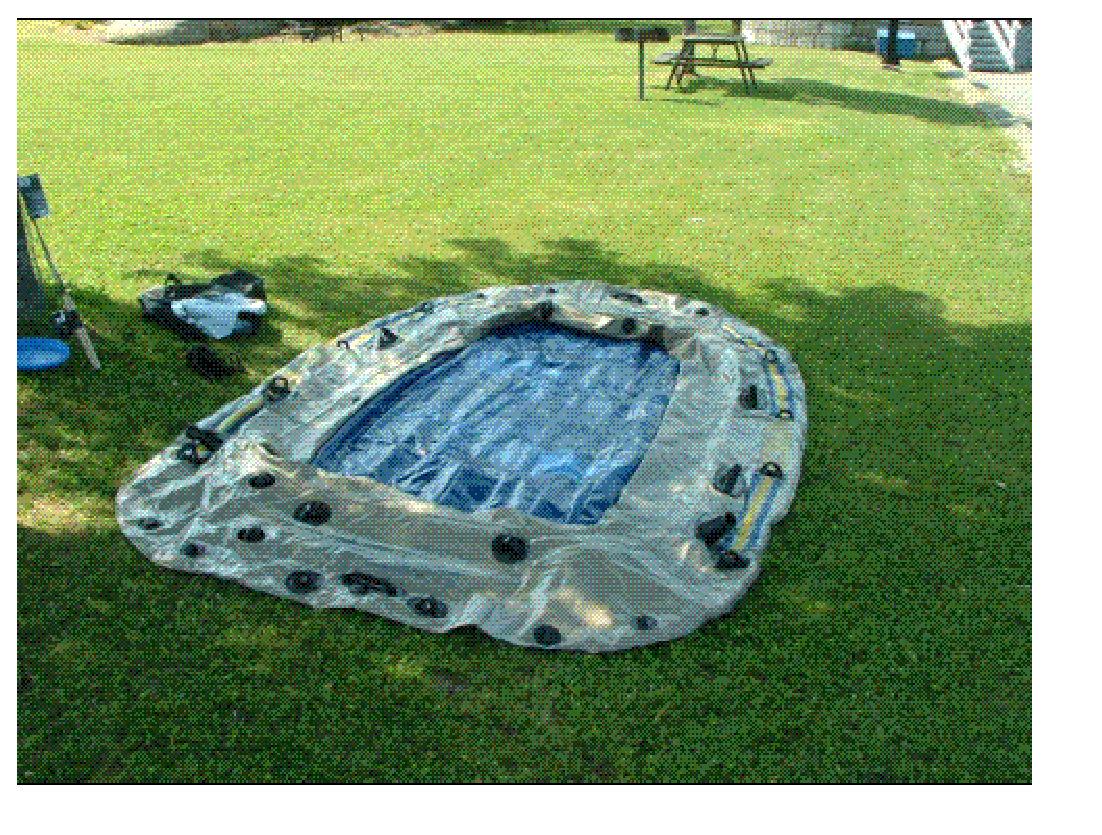
\epsfig{file=fig1.eps,width=3.5in}
Which one of the following is missing in it?
 
 
\noindent{\textbf{\large{
A.}}}
Lawn
 
 
\noindent{\textbf{\large{
B.}}}
A table
 
 
\noindent{\textbf{\large{
C.}}}
A truck
 
 
\noindent{\textbf{\large{
D.}}}
An airplane
 
 
\noindent{\textbf{\large{
E.}}}
A frisbee
 
 
\noindent{\textbf{\large{
F.}}}
  Not any of aboves.
 
 
\noindent\vspace{0.05in}{\textbf{\Large{Auto-answer:}}}
 
 
\noindent{\textbf{\large{
C.}}}
A truck
 
 
\noindent{\textbf{\large{
D.}}}
An airplane
 
 
\noindent\vspace{0.05in}{\textbf{\Large{End of auto-answer.}}}
 
 
 
\vspace{0.3in}
   
   
\noindent{\textbf{\Large{Total numbers: }}}
   
   
\noindent\begin{tabular}{|l|l|l|l|l|l|l|}
 \hline
Inputs & Calculates & Choices & Layers & Matches & Answer & Solution \\ \hline
           0 & 
           0 & 
           6
  simple  
  & 
           6 & 
           0 & 
  yes & 
  no 
  \\ \hline
 \end{tabular}
   
   
   
   
\noindent\vspace{0.1in}{\textbf{\Large{Calculated values:}}}
   
   
   
   
\noindent\vspace{0.1in}\hspace{-0.08in} {\textbf{\Large{All inputs: }}}
   
   
  
\vspace{0.2in}
  
{\textbf{\Large{Question
30.1.6 
 (          6,         13,         28)
}}}
  
  
What is the operation between $a= % 
5$ and $b= % 
2$:
$a$  % 
$+$ $b=?$ Please also calculate it.
 
 
\noindent\vspace{0.05in}{\textbf{\Large{Answer:}}}
 
 

5;
 
2;
 
The operation is  % 
ADDITION and the result is
$ % 
7.0000$.
 
 
 
\noindent\vspace{0.05in}{\textbf{\Large{End of Answer.}}}
 
 

 
\vspace{0.3in}
   
   
\noindent{\textbf{\Large{Total numbers: }}}
   
   
\noindent\begin{tabular}{|l|l|l|l|l|l|l|}
 \hline
Inputs & Calculates & Choices & Layers & Matches & Answer & Solution \\ \hline
           3 & 
           2 & 
           0
  & 
           0 & 
           0 & 
  yes & 
  no 
  \\ \hline
 \end{tabular}
   
   
   
   
\noindent\vspace{0.1in}{\textbf{\Large{Calculated values:}}}
   
   
  
  
\noindent\begin{tabular}{|l|l|l|l|}
\hline
 Sequential & Type & Accuracy & Calculated \\ 
\hline
 
 
  Calculated $           1$ & string & $           1 $ ( $          4 $ strings)
 : 
 & ADDITION
 \\  \hline  
 
 
  Calculated $           2$ & real & $           5 $ & 
 $ 7.0000 $ 
 \\  \hline  
 \end{tabular}
   
   
   
   
\noindent\vspace{0.1in}\hspace{-0.08in} {\textbf{\Large{All inputs: }}}
   
   
  
  
\noindent\begin{tabular}{|l|l|l|l|l|}
\hline
 Sequential & Type & Accuracy & Three inputs & Generated \\ 
\hline
 
 
  INPUT $           1$ & integer &  & $
 1
 , 
 10
 , 
 2
 $ & $ 5 $ 
 \\  \hline  
 
 
  INPUT $           2$ & integer &  & $
 2
 , 
 10
 , 
 2
 $ & $ 2 $ 
 \\  \hline  
 
 
  INPUT $           3$ & string & & 
 $+$ & 
  $ <-- $ 
  \\
  & & & 
 $-$ & 
  \\
  & & & 
 $\times$ & 
  \\
  & & & 
 $\div$ & 
 \\  \hline  
 \end{tabular}
   
   
   
   
\vspace{0.3in}
{\textbf{\LARGE{You have done all the above? A very good beginning, please go ahead.}}}
More constants the
Mass of electron
$m_e$$ =
9.109390 \times 10^{-31} $
kg
,
Universal gas constant
$R$$ =
8.315 $
J/(mol$\cdot $K)
,
$e$$ =
1.60217733 \times 10^{-19} $
C
, and
$m_p$$ =
1.6726231 \times 10^{-27} $
kg
%
may be very helpful.
\vspace{0.3in}
   
   
  
\vspace{0.2in}
  
{\textbf{\Large{QUESTION
30.2 
 (          4,          4,          4)
}}}
  
  
Considering case-insensitivity, please match the following same strings.
  
  
\begin{tabular}{|l|l|l|}
 \hline
 Column Left & Column Right  & Your choinces \\ 
 \hline
{\textbf{\large{
A.}}}
C
  & 
YJH
 & 
 \\ 
 \hline
{\textbf{\large{
B.}}}
er
  & 
ER
 & 
 \\ 
 \hline
{\textbf{\large{
C.}}}
Er
  & 
c
 & 
 \\ 
 \hline
{\textbf{\large{
D.}}}
yjh
  & 
 a= %
3
 & 
 \\ 
 \hline
{\textbf{\large{
E.}}}
 A= %
6/ %
2

  & 
eR
 & 
 \\ 
 \hline
 \end{tabular}
  
  
 
 
\noindent\vspace{0.05in}{\textbf{\Large{Auto-answer:}}}
  
  
\begin{tabular}{|l|l|l|}
 \hline
 Column Left & Column Right  & Answers       \\ 
 \hline
{\textbf{\large{
A.}}}
C
  & 
YJH
 & 
{\textbf{\large{
D.}}}
 \\ 
 \hline
{\textbf{\large{
B.}}}
er
  & 
ER
 & 
{\textbf{\large{
B.}}}
, 
{\textbf{\large{
C.}}}
 \\ 
 \hline
{\textbf{\large{
C.}}}
Er
  & 
c
 & 
{\textbf{\large{
A.}}}
 \\ 
 \hline
{\textbf{\large{
D.}}}
yjh
  & 
 a= %
3
 & 
{\textbf{\large{
E.}}}
 \\ 
 \hline
{\textbf{\large{
E.}}}
 A= %
6/ %
2

  & 
eR
 & 
{\textbf{\large{
B.}}}
, 
{\textbf{\large{
C.}}}
 \\ 
 \hline
 \end{tabular}
  
  
 
 
\noindent\vspace{0.05in}{\textbf{\Large{End of auto-answer.}}}
 
 
 
   
   
\noindent{\textbf{\Large{Total numbers: }}}
   
   
\noindent\begin{tabular}{|l|l|l|l|l|l|l|}
 \hline
Inputs & Calculates & Choices & Layers & Matches & Answer & Solution \\ \hline
           2 & 
           1 & 
           0
  & 
          16 & 
           5 & 
  yes & 
  no 
  \\ \hline
 \end{tabular}
   
   
   
   
\noindent\vspace{0.1in}{\textbf{\Large{Calculated values:}}}
   
   
  
  
\noindent\begin{tabular}{|l|l|l|l|}
\hline
 Sequential & Type & Accuracy & Calculated \\ 
\hline
 
 
  Calculated $           1$ & integer &  & 
  $ 3 $ 
 \\  \hline  
 \end{tabular}
   
   
   
   
\noindent\vspace{0.1in}\hspace{-0.08in} {\textbf{\Large{All inputs: }}}
   
   
  
  
\noindent\begin{tabular}{|l|l|l|l|l|}
\hline
 Sequential & Type & Accuracy & Three inputs & Generated \\ 
\hline
 
 
  INPUT $           1$ & integer &  & $
 2
 , 
 8
 , 
 2
 $ & $ 6 $ 
 \\  \hline  
 
 
  INPUT $           2$ & integer &  & $
 2
 , 
 3
 , 
 2
 $ & $ 2 $ 
 \\  \hline  
 \end{tabular}
   
   
  
\vspace{0.2in}
  
{\textbf{\Large{QUESTION
30.3 
 (          3,          3,          3)
}}}
  
  
Please choose the correct one from the following statements:
 
 
\noindent{\textbf{\large{
A.}}}
Canada has  %
36 provinces and  %
35 territories.
 
 
\noindent{\textbf{\large{
B.}}}
Canada has  %
10 provinces and  %
3 territories.
 
 
\noindent{\textbf{\large{
C.}}}
Canada has  %
34 provinces and  %
39 territories.
 
 
\noindent{\textbf{\large{
D.}}}
Canada has  %
37 provinces and  %
37 territories.
 
 
\noindent{\textbf{\large{
E.}}}
Canada has  %
35 provinces and  %
34 territories.
 
 
\noindent{\textbf{\large{
F.}}}
 None of above.
 
 
\noindent\vspace{0.05in}{\textbf{\Large{Auto-answer:}}}
 
 
\noindent{\textbf{\large{
B.}}}
Canada has  %
10 provinces and  %
3 territories.
 
 
\noindent\vspace{0.05in}{\textbf{\Large{End of auto-answer.}}}
 
 
   
   
\noindent{\textbf{\Large{Total numbers: }}}
   
   
\noindent\begin{tabular}{|l|l|l|l|l|l|l|}
 \hline
Inputs & Calculates & Choices & Layers & Matches & Answer & Solution \\ \hline
           0 & 
          20 & 
           6
  simple  
  & 
           6 & 
           0 & 
  yes & 
  no 
  \\ \hline
 \end{tabular}
   
   
   
   
\noindent\vspace{0.1in}{\textbf{\Large{Calculated values:}}}
   
   
  
  
\noindent\begin{tabular}{|l|l|l|l|}
\hline
 Sequential & Type & Accuracy & Calculated \\ 
\hline
 
 
  Calculated $           1$ & integer &  & 
  $ 10 $ 
 \\  \hline  
 
 
  Calculated $           2$ & integer &  & 
  $ 3 $ 
 \\  \hline  
 
 
  Calculated $           3$ & integer &  & 
  $ 23 $ 
 \\  \hline  
 
 
  Calculated $           4$ & integer &  & 
  $ 24 $ 
 \\  \hline  
 
 
  Calculated $           5$ & integer &  & 
  $ 25 $ 
 \\  \hline  
 
 
  Calculated $           6$ & integer &  & 
  $ 26 $ 
 \\  \hline  
 
 
  Calculated $           7$ & integer &  & 
  $ 27 $ 
 \\  \hline  
 
 
  Calculated $           8$ & integer &  & 
  $ 28 $ 
 \\  \hline  
 
 
  Calculated $           9$ & integer &  & 
  $ 29 $ 
 \\  \hline  
 
 
  Calculated $          10$ & integer &  & 
  $ 30 $ 
 \\  \hline  
 \end{tabular}
   
   
  
  
\noindent\begin{tabular}{|l|l|l|l|}
\hline
 Sequential & Type & Accuracy & Calculated \\ 
\hline
 
 
  Calculated $          11$ & integer &  & 
  $ 31 $ 
 \\  \hline  
 
 
  Calculated $          12$ & integer &  & 
  $ 32 $ 
 \\  \hline  
 
 
  Calculated $          13$ & integer &  & 
  $ 33 $ 
 \\  \hline  
 
 
  Calculated $          14$ & integer &  & 
  $ 34 $ 
 \\  \hline  
 
 
  Calculated $          15$ & integer &  & 
  $ 35 $ 
 \\  \hline  
 
 
  Calculated $          16$ & integer &  & 
  $ 36 $ 
 \\  \hline  
 
 
  Calculated $          17$ & integer &  & 
  $ 37 $ 
 \\  \hline  
 
 
  Calculated $          18$ & integer &  & 
  $ 38 $ 
 \\  \hline  
 
 
  Calculated $          19$ & integer &  & 
  $ 39 $ 
 \\  \hline  
 
 
  Calculated $          20$ & integer &  & 
  $ 40 $ 
 \\  \hline  
 \end{tabular}
   
   
   
   
\noindent\vspace{0.1in}\hspace{-0.08in} {\textbf{\Large{All inputs: }}}
   
   
  
\vspace{0.2in}
  
{\textbf{\Large{QUESTION
30.4 
 (          1,          1,          1)
}}}
  
  


\noindent\vspace{0.05in}{\textbf{\Large{Abstract:}}}
This is a simple Newton's Second Law calculation multi-choice problem.  
\noindent\vspace{0.05in}{\textbf{\Large{end of abstract.}}}


 
 
An object is subjected to an external net force $\mathbf{f}=
(30.0 , 8.0 , -7000.0) N$.
Its mass is known as $m= % 
56.0000 kg$. Please choose the
correct accelaration from the following choices.
 
 
 
\noindent{\textbf{\large{
A.}}}
The accelaration is $  %
(
-3.63,
-.69,
-125.00)
ms^{-2} $.
 
 
\noindent{\textbf{\large{
B.}}}
The accelaration is $  %
(
-3.63,
.14,
-125.00)
ms^{-2} $.
 
 
\noindent{\textbf{\large{
C.}}}
The accelaration is $  %
(
-3.63,
-.69,
570.50)
ms^{-2} $.
 
 
\noindent{\textbf{\large{
D.}}}
The accelaration is $  %
(
.536,
-.69,
570.50)
ms^{-2} $.
 
 
\noindent{\textbf{\large{
E.}}}
The accelaration is $  %
(
.536,
.14,
-125.00)
ms^{-2} $.
 
 
\noindent{\textbf{\large{
F.}}}
The accelaration is $  %
(
.536,
.14,
570.50)
ms^{-2} $.
 
 
\noindent{\textbf{\large{
G.}}}
The accelaration is $  %
(
-3.63,
.14,
570.50)
ms^{-2} $.
 
 
\noindent{\textbf{\large{
H.}}}
The accelaration is $  %
(
.536,
-.69,
-125.00)
ms^{-2} $.
 
 
\noindent\vspace{0.05in}{\textbf{\Large{Auto-answer:}}}
 
 
\noindent{\textbf{\large{
E.}}}
The accelaration is $  %
(
.536,
.14,
-125.00)
ms^{-2} $.
 
 
\noindent\vspace{0.05in}{\textbf{\Large{End of auto-answer.}}}
 
 
 
 
 
\noindent\vspace{0.05in}{\textbf{\Large{Answer:}}}
 
 

The correct answer from the choices is


\noindent{\textbf{\large{
E.}}}
The accelaration is $  %
(
.536,
.14,
-125.00)
ms^{-2} $.
 
 
 
\noindent\vspace{0.05in}{\textbf{\Large{End of Answer.}}}
 
 

 
 
 
\noindent\vspace{0.1in}{\textbf{\Large{Solution: }}}
 
 

We will use the Newton's Second Law:
 
\[
\mathbf{f}=m\mathbf{a}.
\]
 
Since $\mathbf{f}= % 
(30.0 , 8.0 , -7000.0) N$
and $m= % 
56.0000kg$, bring them into the above equation, then we get
 
\begin{eqnarray*}
\mathbf{a}&=&\frac{\mathbf{f}}m  \\
&=&\frac{ % 
(30.0 , 8.0 , -7000.0) N}{ % 
56.0000kg}  \\
&=& % 
(.536 , .14 , -125.00) ms^{-2}
\end{eqnarray*}
 
 
 
\noindent\vspace{0.1in}{\textbf{\Large{End of Solution.}}}
 
 

 
\vspace{0.3in}
   
   
\noindent{\textbf{\Large{Total numbers: }}}
   
   
\noindent\begin{tabular}{|l|l|l|l|l|l|l|}
 \hline
Inputs & Calculates & Choices & Layers & Matches & Answer & Solution \\ \hline
           2 & 
           1 & 
           8
  & 
           3 & 
           0 & 
  yes & 
  yes 
  \\ \hline
 \end{tabular}
   
   
   
   
\noindent\vspace{0.1in}{\textbf{\Large{Calculated values:}}}
   
   
  
  
\noindent\begin{tabular}{|l|l|l|l|}
\hline
 Sequential & Type & Accuracy & Calculated \\ 
\hline
 
 
  Calculated $           1$ & vector &  
  $           3 $ 
 &  $ .536 $ 
 \\    
  & & 
  $           2 $ 
 &  $ .14 $ 
 \\    
  & & 
  $           5 $ 
 &  $ -125.00 $ 
 \\  \hline  
 \end{tabular}
   
   
   
   
\noindent\vspace{0.1in}\hspace{-0.08in} {\textbf{\Large{All inputs: }}}
   
   
  
  
\noindent\begin{tabular}{|l|l|l|l|l|}
\hline
 Sequential & Type & Accuracy & Three inputs & Generated \\ 
\hline
 
 
  INPUT $           1$ & vector & $          -1 $ & $
20.0
  $ & \\
  & & & $
101.0
  $ & \\
  & & & $
10.0
$ & $ 30.0 $ 
  \\
  & & $          -1 $ & $
2.0
  $ & \\
  & & & $
10.1
  $ & \\
  & & & $
1.0
$ & $ 8.0 $ 
  \\
  & & $          -1 $ & $
-2000.0
  $ & \\
  & & & $
-10001.0
  $ & \\
  & & & $
-1000.0
$ & $ -7000.0 $ 
 \\  \hline  
 
 
  INPUT $           2$ & real & $          -4 $ & $
 50.0000
  $ & \\
  & & &  $
 60.1000
  $ & \\
  & & &  $
 2.0000
 $ & $ 56.0000 $ 
 \\  \hline  
 \end{tabular}
   
   
  
\vspace{0.2in}
  
{\textbf{\Large{QUESTION
30.5 
 (          5,          5,          5)
}}}
  
  
If any one of the following statements is correct, please fill the box ahead of it with $T$ .
If wrong, fill with $F$.
 
\noindent\begin{tabular}{|l|l|}\hline Your&\hspace{.2in} \\ answer&\hspace{.2in} \\ \hline \end{tabular}
1. $ % 
28$ is an  % 
even number.
 
\noindent\begin{tabular}{|l|l|}\hline Your&\hspace{.2in} \\ answer&\hspace{.2in} \\ \hline \end{tabular}
2.  % 
Montreal is in  % 
Quebec province.
 
\noindent\begin{tabular}{|l|l|}\hline Your&\hspace{.2in} \\ answer&\hspace{.2in} \\ \hline \end{tabular}
3.  % 
$\mathbf{F}=m\mathbf{a}$ is a mathmatical form of
the Newton's Second Law.
 
 
 
\noindent\vspace{0.05in}{\textbf{\Large{Answer:}}}
 
 

 
\noindent\begin{tabular}{|l|l|}\hline The correct & \\
          answer &  % 
$T$ \\ \hline \end{tabular}
1. $ % 
28$ is an  % 
even number.
 
\noindent\begin{tabular}{|l|l|}\hline The correct & \\
          answer &  % 
$T$ \\ \hline \end{tabular}
2.  % 
Montreal is in  % 
Quebec province.
 
\noindent\begin{tabular}{|l|l|}\hline The correct & \\
          answer &  % 
$T$ \\ \hline \end{tabular}
3.  % 
$\mathbf{F}=m\mathbf{a}$ is a mathmatical form of  % 
the Newton's Second Law.
 
 
 
\noindent\vspace{0.05in}{\textbf{\Large{End of Answer.}}}
 
 

 
\vspace{0.3in}
   
   
\noindent{\textbf{\Large{Total numbers: }}}
   
   
\noindent\begin{tabular}{|l|l|l|l|l|l|l|}
 \hline
Inputs & Calculates & Choices & Layers & Matches & Answer & Solution \\ \hline
           6 & 
           3 & 
           0
  & 
           0 & 
           0 & 
  yes & 
  no 
  \\ \hline
 \end{tabular}
   
   
   
   
\noindent\vspace{0.1in}{\textbf{\Large{Calculated values:}}}
   
   
  
  
\noindent\begin{tabular}{|l|l|l|l|}
\hline
 Sequential & Type & Accuracy & Calculated \\ 
\hline
 
 
  Calculated $           1$ & string & $           1 $ ( $          2 $ strings)
 : 
 & $T$
 \\  \hline  
 
 
  Calculated $           2$ & string & $           1 $ ( $          2 $ strings)
 : 
 & $T$
 \\  \hline  
 
 
  Calculated $           3$ & string & $           1 $ ( $          2 $ strings)
 : 
 & $T$
 \\  \hline  
 \end{tabular}
   
   
   
   
\noindent\vspace{0.1in}\hspace{-0.08in} {\textbf{\Large{All inputs: }}}
   
   
  
  
\noindent\begin{tabular}{|l|l|l|l|l|}
\hline
 Sequential & Type & Accuracy & Three inputs & Generated \\ 
\hline
 
 
  INPUT $           1$ & integer &  & $
 1
 , 
 100
 , 
 1
 $ & $ 28 $ 
 \\  \hline  
 
 
  INPUT $           2$ & string & & 
 even & 
  $ <-- $ 
  \\
  & & & 
 odd & 
 \\  \hline  
 
 
  INPUT $           3$ & string & & 
 Toronto & 
  \\
  & & & 
 Kingston & 
  \\
  & & & 
 Montreal & 
  $ <-- $ 
  \\
  & & & 
 Hull & 
 \\  \hline  
 \end{tabular}
   
   
  
  
\noindent\begin{tabular}{|l|l|l|l|l|}
\hline
 Sequential & Type & Accuracy & Three inputs & Generated \\ 
\hline
 
 
  INPUT $           4$ & string & & 
 Ontario & 
  \\
  & & & 
 Quebec & 
  $ <-- $ 
 \\  \hline  
 
 
  INPUT $           5$ & string & & 
 $\mathbf{F}=m\mathbf{a}$ & 
  $ <-- $ 
  \\
  & & & 
 $\left| \mathbf{F}\right| =Gm_1m_2r^{-2}$ & 
 \\  \hline  
 
 
  INPUT $           6$ & string & & 
 the Newton's Second Law & 
  $ <-- $ 
  \\
  & & & 
 Newton's Law of Universal Gravitation & 
 \\  \hline  
 \end{tabular}
   
   
  
\vspace{0.2in}
  
{\textbf{\Large{QUESTION
30.6 
 (          2,          2,          2)
}}}
  
  
 
An object is subjected to an external net force $\mathbf{f}=(
80.000 ,
5.0000,
-9000.0  )N$. Its mass is known as
$m= % 
54.0000  kg$. Please choose the correct accelaration
from the following choices.
 
 
 
\noindent{\textbf{\large{
A.}}}
The accelaration is
$(
5.6440ms^{-2},
-3602.7km/h^2,
-166.67ms^{-2}
).
$
 
 
\noindent{\textbf{\large{
B.}}}
The accelaration is
$(
1.4815ms^{-2},
1200.0km/h^2,
-166.67ms^{-2}
).
$
 
 
\noindent{\textbf{\large{
C.}}}
The accelaration is
$(
1.4815ms^{-2},
1200.0km/h^2,
-709.22ms^{-2}
).
$
 
 
\noindent{\textbf{\large{
D.}}}
The accelaration is
$(
5.6440ms^{-2},
-3602.7km/h^2,
-709.22ms^{-2}
).
$
 
 
\noindent{\textbf{\large{
E.}}}
The accelaration is
$(
1.4815ms^{-2},
-3602.7km/h^2,
-166.67ms^{-2}
).
$
 
 
\noindent{\textbf{\large{
F.}}}
The accelaration is
$(
1.4815ms^{-2},
-3602.7km/h^2,
-709.22ms^{-2}
).
$
 
 
\noindent{\textbf{\large{
G.}}}
 None of these.
 
 
\noindent\vspace{0.05in}{\textbf{\Large{Auto-answer:}}}
 
 
\noindent{\textbf{\large{
B.}}}
The accelaration is
$(
1.4815ms^{-2},
1200.0km/h^2,
-166.67ms^{-2}
).
$
 
 
\noindent\vspace{0.05in}{\textbf{\Large{End of auto-answer.}}}
 
 
 
 
 
 
\noindent\vspace{0.1in}{\textbf{\Large{Solution: }}}
 
 

We will use the Newton's Second Law:
 
\[
\mathbf{f}=m\mathbf{a}.
\]
 
Since $\mathbf{f}=( % 
80.000,  % 
5.0000,  % 
-9000.0 )N$
and $m= % 
54.0000kg$, bring them into the above equation, then we get
 
\begin{eqnarray*}
\mathbf{a}&=&\frac{\mathbf{f}}m  \\
&=&\frac{(
80.000 ,
5.0000 ,
-9000.0 )N
}{ % 
54.0000 kg}  \\
&=&(
1.4815 ,
9.2593 \times 10^{-2},
-166.67
)ms^{-2} \\
&=&(
19200. ,
1200.0 ,
-2.1600 \times 10^{6}
)km/h^2.
\end{eqnarray*}
 
 
 
\noindent\vspace{0.1in}{\textbf{\Large{End of Solution.}}}
 
 

 
\vspace{0.3in}
   
   
\noindent{\textbf{\Large{Total numbers: }}}
   
   
\noindent\begin{tabular}{|l|l|l|l|l|l|l|}
 \hline
Inputs & Calculates & Choices & Layers & Matches & Answer & Solution \\ \hline
           4 & 
           6 & 
           7
  & 
           3 & 
           0 & 
  yes & 
  yes 
  \\ \hline
 \end{tabular}
   
   
   
   
\noindent\vspace{0.1in}{\textbf{\Large{Calculated values:}}}
   
   
  
  
\noindent\begin{tabular}{|l|l|l|l|}
\hline
 Sequential & Type & Accuracy & Calculated \\ 
\hline
 
 
  Calculated $           1$ & real & $           5 $ & 
 $ 1.4815 $ 
 \\  \hline  
 
 
  Calculated $           2$ & real & $           5 $ & 
 $ 9.2593 \times 10^{-2} $ 
 \\  \hline  
 
 
  Calculated $           3$ & real & $           5 $ & 
 $ -166.67 $ 
 \\  \hline  
 
 
  Calculated $           4$ & real & $           5 $ & 
 $ 19200. $ 
 \\  \hline  
 
 
  Calculated $           5$ & real & $           5 $ & 
 $ 1200.0 $ 
 \\  \hline  
 
 
  Calculated $           6$ & real & $           5 $ & 
 $ -2.1600 \times 10^{6} $ 
 \\  \hline  
 \end{tabular}
   
   
   
   
\noindent\vspace{0.1in}\hspace{-0.08in} {\textbf{\Large{All inputs: }}}
   
   
  
  
\noindent\begin{tabular}{|l|l|l|l|l|}
\hline
 Sequential & Type & Accuracy & Three inputs & Generated \\ 
\hline
 
 
  INPUT $           1$ & real & $          -3 $ & $
 20.000
  $ & \\
  & & &  $
 101.000
  $ & \\
  & & &  $
 10.000
 $ & $ 80.000 $ 
 \\  \hline  
 
 
  INPUT $           2$ & real & $          -4 $ & $
 2.0000
  $ & \\
  & & &  $
 10.1000
  $ & \\
  & & &  $
 1.0000
 $ & $ 5.0000 $ 
 \\  \hline  
 
 
  INPUT $           3$ & real & $          -1 $ & $
 -2000.0
  $ & \\
  & & &  $
 -10001.0
  $ & \\
  & & &  $
 -1000.0
 $ & $ -9000.0 $ 
 \\  \hline  
 \end{tabular}
   
   
  
  
\noindent\begin{tabular}{|l|l|l|l|l|}
\hline
 Sequential & Type & Accuracy & Three inputs & Generated \\ 
\hline
 
 
  INPUT $           4$ & real & $          -4 $ & $
 50.0000
  $ & \\
  & & &  $
 60.1000
  $ & \\
  & & &  $
 2.0000
 $ & $ 54.0000 $ 
 \\  \hline  
 \end{tabular}
   
   
   
   
\vspace{0.3in}
{\textbf{\LARGE{You have done all the above? Excellent! Not much left, please continue.}}}
\vspace{0.3in}
   
   
  
\vspace{0.2in}
  
{\textbf{\Large{QUESTION
30.7 
 (          8,         15,         60)
}}}
  
  
 
$ \left( \begin{array}{ccccccccc}
           7 & 
           4 & 
           5 & 
           7 \\ 
           4 & 
           5 & 
           6 & 
           4 \\ 
           7 & 
           5 & 
           5 & 
           7
\end{array}\right) \times
\left( \begin{array}{c}
           2 \\ 
           2 \\ 
           2 \\ 
           2
\end{array}\right) $ =?
 
 
$  % 
 \left( \begin{array}
 {
 c
 c
 }
 \rho & 
 \beta \\ 
                    \zeta & 
 \Theta \\ 
 \Lambda & 
 \Psi \\ 
 \Gamma & 
 \Gamma
 \end{array} \right)
 \left( \begin{array}
 {
 c
 }
 \beta \\ 
 \beta
 \end{array} \right)
$ =?
 
 
 
\noindent\vspace{0.05in}{\textbf{\Large{Answer:}}}
 
 

 
$\left( \begin{array}{ccccccccccccccc}
           7 & 
           4 & 
           5 & 
           7 \\ 
           4 & 
           5 & 
           6 & 
           4 \\ 
           7 & 
           5 & 
           5 & 
           7
\end{array}\right) \times
\left( \begin{array}{c}
           2 \\ 
           2 \\ 
           2 \\ 
           2
\end{array}\right)  =
\left( \begin{array}{c}
          46 \\ 
          38 \\ 
          48
\end{array}\right)  $
 
$  % 
 \left( \begin{array}
 {
 c
 c
 }
 \rho & 
 \beta \\ 
                    \zeta & 
 \Theta \\ 
 \Lambda & 
 \Psi \\ 
 \Gamma & 
 \Gamma
 \end{array} \right)
 \left( \begin{array}
 {
 c
 }
 \beta \\ 
 \beta
 \end{array} \right)
=
  \left( \begin{array}
 {
 c
 }
 \rho \times  \beta   +  \beta \times  \beta \\ 
                    \zeta \times  \beta   +  \Theta \times  \beta \\ 
 \Lambda \times  \beta   +  \Psi \times  \beta \\ 
 \Gamma \times  \beta   +  \Gamma \times  \beta
 \end{array} \right)
$
 
 
 
\noindent\vspace{0.05in}{\textbf{\Large{End of Answer.}}}
 
 

 
 
 
\noindent\vspace{0.1in}{\textbf{\Large{Solution: }}}
 
 

 
 
\noindent\vspace{0.1in}{\textbf{\Large{End of Solution.}}}
 
 

 
\vspace{0.3in}
   
   
\noindent{\textbf{\Large{Total numbers: }}}
   
   
\noindent\begin{tabular}{|l|l|l|l|l|l|l|}
 \hline
Inputs & Calculates & Choices & Layers & Matches & Answer & Solution \\ \hline
           4 & 
           2 & 
           0
  & 
           0 & 
           0 & 
  yes & 
  yes 
  \\ \hline
 \end{tabular}
   
   
   
   
\noindent\vspace{0.1in}{\textbf{\Large{Calculated values:}}}
   
   
  
  
\noindent\begin{tabular}{|l|l|l|l|}
\hline
 Sequential & Type & Accuracy & Calculated \\ 
\hline
 
 
  Calculated $           1$ & i-matrix &  & 
 (size:           3 by           1)
 \\  \hline  
 \end{tabular}
   
   
$\begin{array}{
 c
 }
          46 \\ 
          38 \\ 
          48
 \end{array}  $ 
  
  
\noindent\begin{tabular}{|l|l|l|l|}
\hline
 Sequential & Type & Accuracy & Calculated \\ 
\hline
 
 
  Calculated $           2$ & s-matrix & & 
 (size:           4 by           1)
 \\  \hline  
 \end{tabular}
   
   
 $   \left( \begin{array}
 {
 c
 }
 \rho \times  \beta   +  \beta \times  \beta \\ 
                    \zeta \times  \beta   +  \Theta \times  \beta \\ 
 \Lambda \times  \beta   +  \Psi \times  \beta \\ 
 \Gamma \times  \beta   +  \Gamma \times  \beta
 \end{array} \right) $ 
   
   
\noindent\vspace{0.1in}\hspace{-0.08in} {\textbf{\Large{All inputs: }}}
   
   
  
  
\noindent\begin{tabular}{|l|l|l|l|l|}
\hline
 Sequential & Type & Accuracy & Three inputs & Generated \\ 
\hline
 
 
  INPUT $           1$ & i-matrix &  & $
 4
 , 
 7
 , 
 1
 $ & (size:           3 by           4)
 \\  \hline  
 \end{tabular}
   
   
 $\begin{array}{
 c
 c
 c
 c
 }
           7 & 
           4 & 
           5 & 
           7 \\ 
           4 & 
           5 & 
           6 & 
           4 \\ 
           7 & 
           5 & 
           5 & 
           7
\end{array}  $ 
  
  
\noindent\begin{tabular}{|l|l|l|l|l|}
\hline
 Sequential & Type & Accuracy & Three inputs & Generated \\ 
\hline
 
 
  INPUT $           2$ & i-matrix &  & $
 2
 , 
 2
 , 
 1
 $ & (size:           4 by           1)
 \\  \hline  
 \end{tabular}
   
   
 $\begin{array}{
 c
 }
           2 \\ 
           2 \\ 
           2 \\ 
           2
\end{array}  $ 
  
  
\noindent\begin{tabular}{|l|l|l|l|l|}
\hline
 Sequential & Type & Accuracy & Three inputs & Generated \\ 
\hline
 
 
  INPUT $           3$ & s-matrix & & 
 $  \alpha $ & 
  \\
  & & & 
 $  \beta $ & 
  \\
  & & & 
 $  \gamma $ & 
  \\
  & & & 
 $  \delta $ & 
  \\
  & & & 
 $  \epsilon $ & 
  \\
  & & & 
 $  \varepsilon $ & 
  \\
  & & & 
 $                     \zeta $ & 
  \\
  & & & 
 $  \eta $ & 
  \\
  & & & 
 $  \rho $ & 
  \\
  & & & 
 $  \sigma $ & 
  \\
  & & & 
 $  \Gamma $ & 
  \\
  & & & 
 $  \Delta $ & 
  \\
  & & & 
 $  \Theta $ & 
  \\
  & & & 
 $  \Lambda $ & 
  \\
  & & & 
 $                     \Xi $ & 
  \\
  & & & 
 $  \Upsilon $ & 
  \\
  & & & 
 $  \Phi $ & 
  \\
  & & & 
 $  \Psi $ & 
  \\
  & & & 
 $  \Omega $ & 
  (size:           4 by           2)
 \\  \hline  
 \end{tabular}
   
   
 $  \left( \begin{array}
 {
 c
 c
 }
 \rho & 
 \beta \\ 
                    \zeta & 
 \Theta \\ 
 \Lambda & 
 \Psi \\ 
 \Gamma & 
 \Gamma
 \end{array} \right) $ 
  
  
\noindent\begin{tabular}{|l|l|l|l|l|}
\hline
 Sequential & Type & Accuracy & Three inputs & Generated \\ 
\hline
 
 
  INPUT $           4$ & s-matrix & & 
 $  \beta $ & 
  \\
  & & & 
 $  \gamma $ & 
  (size:           2 by           1)
 \\  \hline  
 \end{tabular}
   
   
 $  \left( \begin{array}
 {
 c
 }
 \beta \\ 
 \beta
 \end{array} \right) $ 
  
\vspace{0.2in}
  
{\textbf{\Large{QUESTION
30.8 
 (          7,         14,         50)
}}}
  
  
 
An object is subjected to an external net force $\mathbf{f}=
(90.0 , 2.0 , -6000.0) N$.
Its mass is known as $m= % 
54.0 kg$.
Please choose the correct accelaration from the following choices.
 
 
\noindent{\textbf{\large{
A.}}}
  The accelaration is $  %
(
-8.24,
.17,
-111.11)
ms^{-2} $.
 
 
\noindent{\textbf{\large{
B.}}}
  The accelaration is $  %
(
-8.24,
3.7 \times 10^{-2},
351.37)
ms^{-2} $.
 
 
\noindent{\textbf{\large{
C.}}}
  The accelaration is $  %
(
1.67,
3.7 \times 10^{-2},
-111.11)
ms^{-2} $.
 
 
\noindent{\textbf{\large{
D.}}}
  The accelaration is $  %
(
-8.24,
.17,
351.37)
ms^{-2} $.
 
 
\noindent\vspace{0.05in}{\textbf{\Large{Auto-answer:}}}
 
 
\noindent{\textbf{\large{
C.}}}
  The accelaration is $  %
(
1.67,
3.7 \times 10^{-2},
-111.11)
ms^{-2} $.
 
 
\noindent\vspace{0.05in}{\textbf{\Large{End of auto-answer.}}}
 
 
 
 
 
\noindent\vspace{0.1in}{\textbf{\Large{Solution: }}}
 
 

We will use the Newton's Second Law:
 
\[
\mathbf{f}=m\mathbf{a}.
\]
 
Since $\mathbf{f}= % 
(90.0 , 2.0 , -6000.0) N$
and $m= % 
54.0kg$, bring them into the above equation, then we get
 
\begin{eqnarray*}
\mathbf{a}&=&\frac{\mathbf{f}}m  \\
&=&\frac{ % 
(90.0 , 2.0 , -6000.0) N}{ % 
54.0kg}  \\
&=& % 
(1.67 , 3.7 \times 10^{-2} , -111.11) ms^{-2}
\end{eqnarray*}
 
 
 
\noindent\vspace{0.1in}{\textbf{\Large{End of Solution.}}}
 
 

 
 
\vspace{0.3in}
   
   
\noindent{\textbf{\Large{Total numbers: }}}
   
   
\noindent\begin{tabular}{|l|l|l|l|l|l|l|}
 \hline
Inputs & Calculates & Choices & Layers & Matches & Answer & Solution \\ \hline
           2 & 
           1 & 
           4
  & 
           3 & 
           0 & 
  yes & 
  yes 
  \\ \hline
 \end{tabular}
   
   
   
   
\noindent\vspace{0.1in}{\textbf{\Large{Calculated values:}}}
   
   
  
  
\noindent\begin{tabular}{|l|l|l|l|}
\hline
 Sequential & Type & Accuracy & Calculated \\ 
\hline
 
 
  Calculated $           1$ & vector &  
  $           3 $ 
 &  $ 1.67 $ 
 \\    
  & & 
  $           2 $ 
 &  $ 3.7 \times 10^{-2} $ 
 \\    
  & & 
  $           5 $ 
 &  $ -111.11 $ 
 \\  \hline  
 \end{tabular}
   
   
   
   
\noindent\vspace{0.1in}\hspace{-0.08in} {\textbf{\Large{All inputs: }}}
   
   
  
  
\noindent\begin{tabular}{|l|l|l|l|l|}
\hline
 Sequential & Type & Accuracy & Three inputs & Generated \\ 
\hline
 
 
  INPUT $           1$ & vector & $          -1 $ & $
20.0
  $ & \\
  & & & $
101.0
  $ & \\
  & & & $
10.0
$ & $ 90.0 $ 
  \\
  & & $          -1 $ & $
2.0
  $ & \\
  & & & $
10.1
  $ & \\
  & & & $
1.0
$ & $ 2.0 $ 
  \\
  & & $          -1 $ & $
-2000.0
  $ & \\
  & & & $
-10001.0
  $ & \\
  & & & $
-1000.0
$ & $ -6000.0 $ 
 \\  \hline  
 
 
  INPUT $           2$ & real & $          -1 $ & $
 50.0
  $ & \\
  & & &  $
 60.1
  $ & \\
  & & &  $
 2.0
 $ & $ 54.0 $ 
 \\  \hline  
 \end{tabular}
   
   
  
\vspace{0.2in}
  
{\textbf{\Large{QUESTION
30.9 
 (          9,         16,         70)
}}}
  
  


\noindent\vspace{0.05in}{\textbf{\Large{Abstract:}}}
Quadratic Equation constructed from the following first two random (input) integers as roots,  
which of course should not show in the exam papers.  
\noindent\vspace{0.05in}{\textbf{\Large{end of abstract.}}}


 
 
% First root
% Second root

 
Please solve the following equation:
\begin{eqnarray*}
-15 \times x^2  % 
-30
                 \times x    % 
+  % 
525 =0
\end{eqnarray*}
 
 
 
\noindent\vspace{0.05in}{\textbf{\Large{Answer:}}}
 
 

5,  % 
-7
 
 
 
\noindent\vspace{0.05in}{\textbf{\Large{End of Answer.}}}
 
 

 
 
 
\noindent\vspace{0.1in}{\textbf{\Large{Solution: }}}
 
 

Roots to the equation
\begin{eqnarray*}
-15 \times x^2  % 
-30
                 \times x    % 
+  % 
525 =0
\end{eqnarray*}
are  % 
5 and  % 
-7 .
 
Let us verity  % 
5 first:
$  % 
-15 \times x^2  % 
-30
                 \times x    % 
+  % 
525
  = % 
-375+( % 
-150)+( % 
525)
  = % 
-525+( % 
525)
  = % 
0
$
 
Then verity  % 
-7:
$  % 
-15 \times x^2  % 
-30
                 \times x    % 
+  % 
525
  = % 
-735+( % 
210)+( % 
525)
  = % 
-525+( % 
525)
  = % 
0
$
 
 
 
\noindent\vspace{0.1in}{\textbf{\Large{End of Solution.}}}
 
 

 
\vspace{0.3in}
   
   
\noindent{\textbf{\Large{Total numbers: }}}
   
   
\noindent\begin{tabular}{|l|l|l|l|l|l|l|}
 \hline
Inputs & Calculates & Choices & Layers & Matches & Answer & Solution \\ \hline
           3 & 
          13 & 
           0
  & 
           0 & 
           0 & 
  yes & 
  yes 
  \\ \hline
 \end{tabular}
   
   
   
   
\noindent\vspace{0.1in}{\textbf{\Large{Calculated values:}}}
   
   
  
  
\noindent\begin{tabular}{|l|l|l|l|}
\hline
 Sequential & Type & Accuracy & Calculated \\ 
\hline
 
 
  Calculated $           1$ & integer &  & 
  $ -15 $ 
 \\  \hline  
 
 
  Calculated $           2$ & string & $           2 $ ( $          2 $ strings)
 : 
 & 
 \\  \hline  
 
 
  Calculated $           3$ & integer &  & 
  $ -30 $ 
 \\  \hline  
 
 
  Calculated $           4$ & string & $           1 $ ( $          2 $ strings)
 : 
 & +
 \\  \hline  
 
 
  Calculated $           5$ & integer &  & 
  $ 525 $ 
 \\  \hline  
 
 
  Calculated $           6$ & integer &  & 
  $ -375 $ 
 \\  \hline  
 
 
  Calculated $           7$ & integer &  & 
  $ -150 $ 
 \\  \hline  
 
 
  Calculated $           8$ & integer &  & 
  $ -525 $ 
 \\  \hline  
 
 
  Calculated $           9$ & integer &  & 
  $ 0 $ 
 \\  \hline  
 
 
  Calculated $          10$ & integer &  & 
  $ -735 $ 
 \\  \hline  
 \end{tabular}
   
   
  
  
\noindent\begin{tabular}{|l|l|l|l|}
\hline
 Sequential & Type & Accuracy & Calculated \\ 
\hline
 
 
  Calculated $          11$ & integer &  & 
  $ 210 $ 
 \\  \hline  
 
 
  Calculated $          12$ & integer &  & 
  $ -525 $ 
 \\  \hline  
 
 
  Calculated $          13$ & integer &  & 
  $ 0 $ 
 \\  \hline  
 \end{tabular}
   
   
   
   
\noindent\vspace{0.1in}\hspace{-0.08in} {\textbf{\Large{All inputs: }}}
   
   
  
  
\noindent\begin{tabular}{|l|l|l|l|l|}
\hline
 Sequential & Type & Accuracy & Three inputs & Generated \\ 
\hline
 
 
  INPUT $           1$ & integer &  & $
 -11
 , 
 30
 , 
 4
 $ & $ 5 $ 
 \\  \hline  
 
 
  INPUT $           2$ & integer &  & $
 -31
 , 
 60
 , 
 3
 $ & $ -7 $ 
 \\  \hline  
 
 
  INPUT $           3$ & integer &  & $
 -15
 , 
 15
 , 
 2
 $ & $ -15 $ 
 \\  \hline  
 \end{tabular}
   
   
   
   
   
   
 \vspace{0.2in}
Here are still some constants for use:
 
 
\noindent\begin{tabular}{|l|l|l|}
\hline
Constant & Symbol & Value \\
\hline
 
Mass of proton &
$m_p$ &
 $ 1.6726231 \times 10^{-27} $
kg \\
\hline
 
Boltzmann's constant &
$k$ &
 $ 1.381 \times 10^{-23} $
J/K \\
\hline
 
\end{tabular}
 
Thank you very much for answering these questions!
 
{\textbf{\large{Please be advised}}} that in this paper there are questions from
30.1 through
30.9.
And any one of them may contain more than one sub-question, thus the total number
of sub-questions here is around 14, of which
13 should be answered.
 
   
   
\vspace{2.0in} PAPER TAIL GENERATED.
   
   
   
   
\vspace{1.0in} 
{\textbf{\large{ *** END OF PAPER, THANKS *** }}} 
   
   
\hspace{1.0in} By: 
         239(         26,          34)
   
   
   
   
\newpage 
\setcounter{page}{ 
    31001 } 
   
   
\noindent{\textbf{\huge{THIS IS THE JOURNAL FOR}}}
   
   
 {\textbf{ \Large{ PAPER NUMBER          31 }}}
   
   
\vspace{0.2in}
   
   
\markboth{Journal NOT for examinees !!! {\today}}{Journal NOT for examinees !!! {\today}}
   
   
   
   
   
   
 \vspace{0.2in}
 
 
{\Huge  THIS IS AN EXAMPLE OF}
 
{\Huge  PERSONALIZED TESTS. }
 
If needed, please use the following constants.
 
 
 
\noindent\begin{tabular}{|l|l|l|}
\hline
Constant & Symbol & Value \\
\hline
Acceleration due to earth's gravity &
$g$ &
 $ 9.80 $
m/s$^2$ \\
\hline
Avogadro's number &
$N_A$ &
 $ 6.0221367 \times 10^{23} $
mol$^{-1}$ \\
\hline
Boltzmann's constant &
$k$ &
 $ 1.380658 \times 10^{-23} $
J/K \\
\hline
Coulomb's constant &
$k$ &
 $ 8.99 \times 10^{9} $
N$\cdot $m$^2$/C$^2$ \\
\hline
Electron charge magnitiude &
$e$ &
 $ 1.60217733 \times 10^{-19} $
C \\
\hline
Permeability of free space &
$\mu _0$ &
 $ 1.25663706 \times 10^{-6} $
T$\cdot $m/A \\
\hline
Permittivity of free space &
$\epsilon _0$ &
 $ 8.854187817 \times 10^{-12} $
C$^2$/(N$\cdot $m$^2$) \\
\hline
Pi &
$\pi$ &
 $ 3.14159265 $
$ $ \\
\hline
Planck's constant &
$h$ &
 $ 6.6260755 \times 10^{-34} $
J$\cdot $s \\
\hline
Mass of electron &
$m_e$ &
 $ 9.1093897 \times 10^{-31} $
kg \\
\hline
\end{tabular}
 
 
\noindent\begin{tabular}{|l|l|l|}
\hline
Constant & Symbol & Value \\
\hline
Mass of neutron &
$m_n$ &
 $ 1.6749286 \times 10^{-27} $
kg \\
\hline
Mass of proton &
$m_p$ &
 $ 1.6726231 \times 10^{-27} $
kg \\
\hline
Speed of light in vacuum &
$c$ &
 $ 299792458. $
m/s \\
\hline
Universal gravitational constant &
$G$ &
 $ 6.67259 \times 10^{-11} $
N$\cdot $m$^2$/kg$^2$ \\
\hline
Universal gas constant &
$R$ &
 $ 8.314510 $
J/(mol$\cdot $K) \\
\hline
\end{tabular}
 
 
{\textbf{\large{Please be advised}}} that in this paper there are questions from
31.1 through
31.9.
And any one of them may contain more than one sub-question, thus the total number
of sub-questions here is around 14, of which
13 should be answered.
 
\vspace{0.3in}
 
 
   
   
 PAPER TITLE GENERATED.
   
   
   
\vspace{0.2in}
   
In this paper, big questions will be generated in the following order: 
   
   
            1(          6)
 ,
            2(          3)
 ,
            3(          4)
 ,
            4(          2)
 ,
            5(          5)
 ,
            6(          1)
 ,
            7(          8)
 ,
            8(          7)
 ,
            9(          9)
 .
  
\vspace{0.2in}
  
{\textbf{\Large{QUESTION
31.1 
 (          6)
}}}
  
  
 
{\textbf{\Large{Please answer ONLY
5 of the following
6 questions (Questions
31.1.1 through
31.1.6). }}}
 
Here are still some constants for use in the following questions:
 
 
\noindent\begin{tabular}{|l|l|l|}
\hline
Constant & Symbol & Value \\
\hline
 
Boltzmann's constant &
$k$ &
 $ 1.381 \times 10^{-23} $
J/K \\
\hline
 
Avogadro's number &
$N_A$ &
 $ 6.022 \times 10^{23} $
mol$^{-1}$ \\
\hline
 
Mass of electron &
$m_e$ &
 $ 9.1093897 \times 10^{-31} $
kg \\
\hline
 
\end{tabular}
 
   
\vspace{0.2in}
   
 In this big question of CHOOSE structure,           6 questions will be generat
 ed: 
  
  
            1(          9,         24)
 ,
            2(         13,         28)
 ,
            3(         11,         26)
 ,
            4(          7,         22)
 ,
            5(          8,         23)
 ,
            6(         12,         27)
 .
  
\vspace{0.2in}
  
{\textbf{\Large{Question
31.1.1 
 (          6,          9,         24)
}}}
  
  
Let us use Newton's Law of Universal Gravitation to calculate the force
of the Sun acting on the eight planets. Let us suppose the mass of the
Sun is $ % 
5.00 \times 10^{24} kg$. With the mass and the
distance to the Sun of each planet in the following table, please fill
the blanks for the forces.
 
\vspace{0.2in}
 
 
\begin{tabular}{|l|l|l|l|}
\hline
The Planet & Mass ($kg$) & Distanace from Sun ($m$) & The Force ($N$)\\
\hline
Mercury  &
           $ % 
7.00000000 \times 10^{24} $   &
             $ % 
5.000000000 \times 10^{24} $    &
\\  \hline
Venus    &
           $ % 
2.00 \times 10^{24} $    &
             $ % 
6.00 \times 10^{24} $    &
\\  \hline
Earth    &
           $ % 
9.00 \times 10^{24} $    &
             $ % 
6.00 \times 10^{24} $    &
\\   \hline
Mars     &
           $ % 
2.00 \times 10^{24} $    &
             $ % 
5.00 \times 10^{24} $    &
\\   \hline
Jupiter  &
           $ % 
5.00 \times 10^{24} $    &
             $ % 
5.00 \times 10^{24} $    &
\\  \hline
Saturn   &
           $ % 
4.00 \times 10^{24}$    &
             $ % 
2.00 \times 10^{24}$    &
\\  \hline
Uranus   &
           $ % 
7.00 \times 10^{24} $    &
             $ % 
2.00 \times 10^{24} $    &
\\  \hline
Neptune  &
           $ % 
4.00 \times 10^{24} $    &
             $ % 
4.00 \times 10^{24} $    &
\\  \hline
 
\end{tabular}
 
 
 
 
\noindent\vspace{0.1in}{\textbf{\Large{Solution: }}}
 
 

By using Newton's Law of Universal Gravitation:
\[
F=G \frac{(Sun's \hspace{0.1in} mass) \times (Planet's \hspace{0.1in} mass)} { (distance)^2},
\]
where
$ G= % 
6.67 \times 10^{-11}N m^{2}(kg)^{-2}$ , the forces can be easily calculated as
 
\vspace{0.2in}
 
 
\begin{tabular}{|l|l|l|l|}
\hline
The Planet & Mass ($kg$) & Distanace from Sun ($m$) & The Force ($N$)\\
\hline
Mercury  &
           $ % 
7.00000000 \times 10^{24} $   &
             $ % 
5.000000000 \times 10^{24} $    & $ % 
9.34 \times 10^{-11} $
\\  \hline
Venus    &
           $  % 
2.00 \times 10^{24}  $     &
             $ % 
6.00 \times 10^{24} $    & $ % 
1.85 \times 10^{-11} $
\\  \hline
Earth    &
           $  % 
9.00 \times 10^{24}  $     &
             $ % 
6.00 \times 10^{24} $    & $ % 
8.34 \times 10^{-11} $
\\   \hline
Mars     &
           $  % 
2.00 \times 10^{24} $     &
             $ % 
5.00 \times 10^{24} $    & $ % 
2.67 \times 10^{-11} $
\\   \hline
Jupiter  &
           $  % 
5.00 \times 10^{24} $    &
             $ % 
5.00 \times 10^{24} $    & $ % 
6.67 \times 10^{-11} $
\\  \hline
Saturn   &
           $  % 
4.00 \times 10^{24} $    &
             $ % 
2.00 \times 10^{24}  $    & $ % 
3.33 \times 10^{-10} $
\\  \hline
Uranus   &
           $  % 
7.00 \times 10^{24} $    &
             $ % 
2.00 \times 10^{24} $    & $ % 
5.84 \times 10^{-10} $
\\  \hline
Neptune  &
           $  % 
4.00 \times 10^{24} $    &
             $ % 
4.00 \times 10^{24} $    & $ % 
8.34 \times 10^{-11} $
\\  \hline
 
\end{tabular}
 
 
 
 
\noindent\vspace{0.1in}{\textbf{\Large{End of Solution.}}}
 
 

 
 
 
 
\noindent\vspace{0.05in}{\textbf{\Large{Answer:}}}
 
 

By using Newton's Law of Universal Gravitation:
\[
F=G \frac{(Sun's \hspace{0.1in} mass) \times (Planet's \hspace{0.1in} mass)} { (distance)^2},
\]
where
$ G= % 
6.67 \times 10^{-11} N m^{2}(kg)^{-2}$ , the forces can be easily calculated as
 
\vspace{0.2in}
 
 
\begin{tabular}{|l|l|l|l|}
\hline
The Planet & Mass ($kg$) & Distanace from Sun ($m$) & The Force ($N$)\\
\hline
Mercury  &
           $ % 
7.00000000 \times 10^{24}  $   &
             $ % 
5.000000000 \times 10^{24}$    & $ % 
9.34 \times 10^{-11} $
\\  \hline
Venus    &
           $  % 
2.00 \times 10^{24}  $     &
             $ % 
6.00 \times 10^{24} $    & $ % 
1.85 \times 10^{-11} $
\\  \hline
Earth    &
           $  % 
9.00 \times 10^{24}$     &
             $ % 
6.00 \times 10^{24} $    & $ % 
8.34 \times 10^{-11} $
\\   \hline
Mars     &
           $  % 
2.00 \times 10^{24} $     &
             $ % 
5.00 \times 10^{24}$    & $ % 
2.67 \times 10^{-11} $
\\   \hline
Jupiter  &
           $  % 
5.00 \times 10^{24}  $    &
             $ % 
5.00 \times 10^{24} $    & $ % 
6.67 \times 10^{-11}3 $
\\  \hline
Saturn   &
           $  % 
4.00 \times 10^{24}   $    &
             $ % 
2.00 \times 10^{24}  $    & $ % 
3.33 \times 10^{-10} $
\\  \hline
Uranus   &
           $  % 
7.00 \times 10^{24} $    &
             $ % 
2.00 \times 10^{24}$    & $ % 
5.84 \times 10^{-10} $
\\  \hline
Neptune  &
           $  % 
4.00 \times 10^{24}  $    &
             $ % 
4.00 \times 10^{24} $    & $ % 
8.34 \times 10^{-11} $
\\  \hline
 
\end{tabular}
 
 
 
 
\noindent\vspace{0.05in}{\textbf{\Large{End of Answer.}}}
 
 

 
\vspace{0.3in}
   
   
\noindent{\textbf{\Large{Total numbers: }}}
   
   
\noindent\begin{tabular}{|l|l|l|l|l|l|l|}
 \hline
Inputs & Calculates & Choices & Layers & Matches & Answer & Solution \\ \hline
          19 & 
           8 & 
           0
  & 
           0 & 
           0 & 
  yes & 
  yes 
  \\ \hline
 \end{tabular}
   
   
   
   
\noindent\vspace{0.1in}{\textbf{\Large{Calculated values:}}}
   
   
  
  
\noindent\begin{tabular}{|l|l|l|l|}
\hline
 Sequential & Type & Accuracy & Calculated \\ 
\hline
 
 
  Calculated $           1$ & real & $           3 $ & 
 $ 9.34 \times 10^{-11} $ 
 \\  \hline  
 
 
  Calculated $           2$ & real & $           3 $ & 
 $ 1.85 \times 10^{-11} $ 
 \\  \hline  
 
 
  Calculated $           3$ & real & $           3 $ & 
 $ 8.34 \times 10^{-11} $ 
 \\  \hline  
 
 
  Calculated $           4$ & real & $           3 $ & 
 $ 2.67 \times 10^{-11} $ 
 \\  \hline  
 
 
  Calculated $           5$ & real & $           3 $ & 
 $ 6.67 \times 10^{-11} $ 
 \\  \hline  
 
 
  Calculated $           6$ & real & $           3 $ & 
 $ 3.33 \times 10^{-10} $ 
 \\  \hline  
 
 
  Calculated $           7$ & real & $           3 $ & 
 $ 5.84 \times 10^{-10} $ 
 \\  \hline  
 
 
  Calculated $           8$ & real & $           3 $ & 
 $ 8.34 \times 10^{-11} $ 
 \\  \hline  
 \end{tabular}
   
   
   
   
\noindent\vspace{0.1in}\hspace{-0.08in} {\textbf{\Large{All inputs: }}}
   
   
  
  
\noindent\begin{tabular}{|l|l|l|l|l|}
\hline
 Sequential & Type & Accuracy & Three inputs & Generated \\ 
\hline
 
 
  INPUT $           1$ & real & $          22 $ & $
 2.00 \times 10^{24}
  $ & \\
  & & &  $
 1.010 \times 10^{25}
  $ & \\
  & & &  $
 10.0 \times 10^{23}
 $ & $ 5.00 \times 10^{24} $ 
 \\  \hline  
 
 
  INPUT $           2$ & real & $          16 $ & $
 2.00000000 \times 10^{24}
  $ & \\
  & & &  $
 1.010000000 \times 10^{25}
  $ & \\
  & & &  $
 10.0000000 \times 10^{23}
 $ & $ 7.00000000 \times 10^{24} $ 
 \\  \hline  
 
 
  INPUT $           3$ & real & $          15 $ & $
 2.000000000 \times 10^{24}
  $ & \\
  & & &  $
 1.0100000000 \times 10^{25}
  $ & \\
  & & &  $
 10.00000000 \times 10^{23}
 $ & $ 5.000000000 \times 10^{24} $ 
 \\  \hline  
 \end{tabular}
   
   
  
  
\noindent\begin{tabular}{|l|l|l|l|l|}
\hline
 Sequential & Type & Accuracy & Three inputs & Generated \\ 
\hline
 
 
  INPUT $           4$ & real & $          22 $ & $
 2.00 \times 10^{24}
  $ & \\
  & & &  $
 1.010 \times 10^{25}
  $ & \\
  & & &  $
 10.0 \times 10^{23}
 $ & $ 2.00 \times 10^{24} $ 
 \\  \hline  
 
 
  INPUT $           5$ & real & $          22 $ & $
 2.00 \times 10^{24}
  $ & \\
  & & &  $
 1.010 \times 10^{25}
  $ & \\
  & & &  $
 10.0 \times 10^{23}
 $ & $ 6.00 \times 10^{24} $ 
 \\  \hline  
 
 
  INPUT $           6$ & real & $          22 $ & $
 2.00 \times 10^{24}
  $ & \\
  & & &  $
 1.010 \times 10^{25}
  $ & \\
  & & &  $
 10.0 \times 10^{23}
 $ & $ 9.00 \times 10^{24} $ 
 \\  \hline  
 \end{tabular}
   
   
  
  
\noindent\begin{tabular}{|l|l|l|l|l|}
\hline
 Sequential & Type & Accuracy & Three inputs & Generated \\ 
\hline
 
 
  INPUT $           7$ & real & $          22 $ & $
 2.00 \times 10^{24}
  $ & \\
  & & &  $
 1.010 \times 10^{25}
  $ & \\
  & & &  $
 10.0 \times 10^{23}
 $ & $ 6.00 \times 10^{24} $ 
 \\  \hline  
 
 
  INPUT $           8$ & real & $          22 $ & $
 2.00 \times 10^{24}
  $ & \\
  & & &  $
 1.010 \times 10^{25}
  $ & \\
  & & &  $
 10.0 \times 10^{23}
 $ & $ 2.00 \times 10^{24} $ 
 \\  \hline  
 
 
  INPUT $           9$ & real & $          22 $ & $
 2.00 \times 10^{24}
  $ & \\
  & & &  $
 1.010 \times 10^{25}
  $ & \\
  & & &  $
 10.0 \times 10^{23}
 $ & $ 5.00 \times 10^{24} $ 
 \\  \hline  
 \end{tabular}
   
   
  
  
\noindent\begin{tabular}{|l|l|l|l|l|}
\hline
 Sequential & Type & Accuracy & Three inputs & Generated \\ 
\hline
 
 
  INPUT $          10$ & real & $          22 $ & $
 2.00 \times 10^{24}
  $ & \\
  & & &  $
 1.010 \times 10^{25}
  $ & \\
  & & &  $
 10.0 \times 10^{23}
 $ & $ 5.00 \times 10^{24} $ 
 \\  \hline  
 
 
  INPUT $          11$ & real & $          22 $ & $
 2.00 \times 10^{24}
  $ & \\
  & & &  $
 1.010 \times 10^{25}
  $ & \\
  & & &  $
 10.0 \times 10^{23}
 $ & $ 5.00 \times 10^{24} $ 
 \\  \hline  
 
 
  INPUT $          12$ & real & $          22 $ & $
 2.00 \times 10^{24}
  $ & \\
  & & &  $
 1.010 \times 10^{25}
  $ & \\
  & & &  $
 10.0 \times 10^{23}
 $ & $ 4.00 \times 10^{24} $ 
 \\  \hline  
 \end{tabular}
   
   
  
  
\noindent\begin{tabular}{|l|l|l|l|l|}
\hline
 Sequential & Type & Accuracy & Three inputs & Generated \\ 
\hline
 
 
  INPUT $          13$ & real & $          22 $ & $
 2.00 \times 10^{24}
  $ & \\
  & & &  $
 1.010 \times 10^{25}
  $ & \\
  & & &  $
 10.0 \times 10^{23}
 $ & $ 2.00 \times 10^{24} $ 
 \\  \hline  
 
 
  INPUT $          14$ & real & $          22 $ & $
 2.00 \times 10^{24}
  $ & \\
  & & &  $
 1.010 \times 10^{25}
  $ & \\
  & & &  $
 10.0 \times 10^{23}
 $ & $ 7.00 \times 10^{24} $ 
 \\  \hline  
 
 
  INPUT $          15$ & real & $          22 $ & $
 2.00 \times 10^{24}
  $ & \\
  & & &  $
 1.010 \times 10^{25}
  $ & \\
  & & &  $
 10.0 \times 10^{23}
 $ & $ 2.00 \times 10^{24} $ 
 \\  \hline  
 \end{tabular}
   
   
  
  
\noindent\begin{tabular}{|l|l|l|l|l|}
\hline
 Sequential & Type & Accuracy & Three inputs & Generated \\ 
\hline
 
 
  INPUT $          16$ & real & $          22 $ & $
 2.00 \times 10^{24}
  $ & \\
  & & &  $
 1.010 \times 10^{25}
  $ & \\
  & & &  $
 10.0 \times 10^{23}
 $ & $ 4.00 \times 10^{24} $ 
 \\  \hline  
 
 
  INPUT $          17$ & real & $          22 $ & $
 2.00 \times 10^{24}
  $ & \\
  & & &  $
 1.010 \times 10^{25}
  $ & \\
  & & &  $
 10.0 \times 10^{23}
 $ & $ 4.00 \times 10^{24} $ 
 \\  \hline  
 
 
  INPUT $          18$ & real & $         -13 $ & $
 6.67 \times 10^{-11}
  $ & \\
  & & &  $
 6.67 \times 10^{-11}
  $ & \\
  & & &  $
 1.00 \times 10^{-11}
 $ & $ 6.67 \times 10^{-11} $ 
 \\  \hline  
 \end{tabular}
   
   
  
  
\noindent\begin{tabular}{|l|l|l|l|l|}
\hline
 Sequential & Type & Accuracy & Three inputs & Generated \\ 
\hline
 
 
  INPUT $          19$ & real & $         -13 $ & $
 6.67 \times 10^{-11}
  $ & \\
  & & &  $
 6.67 \times 10^{-11}
  $ & \\
  & & &  $
 1.00 \times 10^{-11}
 $ & $ 6.67 \times 10^{-11} $ 
 \\  \hline  
 \end{tabular}
   
   
  
\vspace{0.2in}
  
{\textbf{\Large{Question
31.1.2 
 (          6,         13,         28)
}}}
  
  
What is the operation between $a= % 
7$ and $b= % 
2$:
$a$  % 
$-$ $b=?$ Please also calculate it.
 
 
\noindent\vspace{0.05in}{\textbf{\Large{Answer:}}}
 
 

7;
 
2;
 
The operation is  % 
SUBTRACTION and the result is
$ % 
5.0000$.
 
 
 
\noindent\vspace{0.05in}{\textbf{\Large{End of Answer.}}}
 
 

 
\vspace{0.3in}
   
   
\noindent{\textbf{\Large{Total numbers: }}}
   
   
\noindent\begin{tabular}{|l|l|l|l|l|l|l|}
 \hline
Inputs & Calculates & Choices & Layers & Matches & Answer & Solution \\ \hline
           3 & 
           2 & 
           0
  & 
           0 & 
           0 & 
  yes & 
  no 
  \\ \hline
 \end{tabular}
   
   
   
   
\noindent\vspace{0.1in}{\textbf{\Large{Calculated values:}}}
   
   
  
  
\noindent\begin{tabular}{|l|l|l|l|}
\hline
 Sequential & Type & Accuracy & Calculated \\ 
\hline
 
 
  Calculated $           1$ & string & $           2 $ ( $          4 $ strings)
 : 
 & SUBTRACTION
 \\  \hline  
 
 
  Calculated $           2$ & real & $           5 $ & 
 $ 5.0000 $ 
 \\  \hline  
 \end{tabular}
   
   
   
   
\noindent\vspace{0.1in}\hspace{-0.08in} {\textbf{\Large{All inputs: }}}
   
   
  
  
\noindent\begin{tabular}{|l|l|l|l|l|}
\hline
 Sequential & Type & Accuracy & Three inputs & Generated \\ 
\hline
 
 
  INPUT $           1$ & integer &  & $
 1
 , 
 10
 , 
 2
 $ & $ 7 $ 
 \\  \hline  
 
 
  INPUT $           2$ & integer &  & $
 2
 , 
 10
 , 
 2
 $ & $ 2 $ 
 \\  \hline  
 
 
  INPUT $           3$ & string & & 
 $+$ & 
  \\
  & & & 
 $-$ & 
  $ <-- $ 
  \\
  & & & 
 $\times$ & 
  \\
  & & & 
 $\div$ & 
 \\  \hline  
 \end{tabular}
   
   
  
\vspace{0.2in}
  
{\textbf{\Large{Question
31.1.3 
 (          6,         11,         26)
}}}
  
  
In a hotel, the possiblity of  % 
smoking customer is
$a =  % 
.970$, and the possiblity of  % 
equal or above 30 years old customer is $ b =  % 
6.00 \times 10^{-2}$.
Please calculate the possiblity of  % 
 non-smoking and  % 
under 30 years old customer.
 
 
 
\noindent\vspace{0.1in}{\textbf{\Large{Solution: }}}
 
 

Since the possiblity of  % 
smoking customer is $ a =  % 
.970 $,
and the possiblity of  % 
equal or above 30 years old customer is $ b =  % 
6.00 \times 10^{-2} $,
the possiblity of  % 
non-smoking customer is $ c = 1.0 - a = 1.0 -
.970
=  % 
3.00 \times 10^{-2} $ and the possiblity of  % 
under 30 years old
customer is $ d = 1.0 - b = 1.0 -  % 
6.00 \times 10^{-2} =  % 
.9400  $.
So the possibility of  % 
 non-smoking and  % 
under 30 years old
customer is $ c \times d =  % 
2.82 \times 10^{-2} $.
 
 
 
\noindent\vspace{0.1in}{\textbf{\Large{End of Solution.}}}
 
 

 
 
 
\noindent\vspace{0.05in}{\textbf{\Large{Answer:}}}
 
 

The possibility of  % 
 non-smoking and  % 
under 30 years old
customer is $ (1-a)(1-b) =  % 
2.82 \times 10^{-2} $.
 
 
\noindent\vspace{0.05in}{\textbf{\Large{End of Answer.}}}
 
 

 
\vspace{0.3in}
   
   
\noindent{\textbf{\Large{Total numbers: }}}
   
   
\noindent\begin{tabular}{|l|l|l|l|l|l|l|}
 \hline
Inputs & Calculates & Choices & Layers & Matches & Answer & Solution \\ \hline
           4 & 
           3 & 
           0
  & 
           0 & 
           0 & 
  yes & 
  yes 
  \\ \hline
 \end{tabular}
   
   
   
   
\noindent\vspace{0.1in}{\textbf{\Large{Calculated values:}}}
   
   
  
  
\noindent\begin{tabular}{|l|l|l|l|}
\hline
 Sequential & Type & Accuracy & Calculated \\ 
\hline
 
 
  Calculated $           1$ & real & $           3 $ & 
 $ 3.00 \times 10^{-2} $ 
 \\  \hline  
 
 
  Calculated $           2$ & real & $           4 $ & 
 $ .9400 $ 
 \\  \hline  
 
 
  Calculated $           3$ & real & $           3 $ & 
 $ 2.82 \times 10^{-2} $ 
 \\  \hline  
 \end{tabular}
   
   
   
   
\noindent\vspace{0.1in}\hspace{-0.08in} {\textbf{\Large{All inputs: }}}
   
   
  
  
\noindent\begin{tabular}{|l|l|l|l|l|}
\hline
 Sequential & Type & Accuracy & Three inputs & Generated \\ 
\hline
 
 
  INPUT $           1$ & logical & .TRUE. & 
 smoking & 
  $ <-- $ 
  \\
  & & .FALSE. & 
  non-smoking & 
 \\  \hline  
 
 
  INPUT $           2$ & real & $          -3 $ & $
 1.0 \times 10^{-2}
  $ & \\
  & & &  $
 1.000
  $ & \\
  & & &  $
 1.0 \times 10^{-2}
 $ & $ .970 $ 
 \\  \hline  
 
 
  INPUT $           3$ & logical & .TRUE. & 
 equal or above 30 years old & 
  $ <-- $ 
  \\
  & & .FALSE. & 
  under 30 years old & 
 \\  \hline  
 \end{tabular}
   
   
  
  
\noindent\begin{tabular}{|l|l|l|l|l|}
\hline
 Sequential & Type & Accuracy & Three inputs & Generated \\ 
\hline
 
 
  INPUT $           4$ & real & $          -4 $ & $
 2.00 \times 10^{-2}
  $ & \\
  & & &  $
 1.0000
  $ & \\
  & & &  $
 2.00 \times 10^{-2}
 $ & $ 6.00 \times 10^{-2} $ 
 \\  \hline  
 \end{tabular}
   
   
  
\vspace{0.2in}
  
{\textbf{\Large{Question
31.1.4 
 (          6,          7,         22)
}}}
  
  
 
An object is subjected to an external net force $\mathbf{f}=(
40.0 ,
8.0,
-2000.0  )N$. Its mass is known as
$m= % 
58.0  kg$. Please choose the correct accelaration
from the following choices.
 
 
 
\noindent{\textbf{\large{
A.}}}
The accelaration (vector) is
$(
41249.,
1787.6 ,
-1.0404 \times 10^{6}
)km/h^2.
$
 
 
\noindent{\textbf{\large{
B.}}}
The accelaration (vector) is
$(
41249.,
1787.6 ,
-446897.
)km/h^2.
$
 
 
\noindent{\textbf{\large{
C.}}}
The accelaration (vector) is
$(
32375.,
1787.6 ,
2.2177 \times 10^{6}
)km/h^2.
$
 
 
\noindent{\textbf{\large{
D.}}}
The accelaration (vector) is
$(
8937.9,
1787.6 ,
-446897.
)km/h^2.
$
 
 
\noindent{\textbf{\large{
E.}}}
The accelaration (vector) is
$(
8937.9,
1787.6 ,
2.2177 \times 10^{6}
)km/h^2.
$
 
 
\noindent{\textbf{\large{
F.}}}
The accelaration (vector) is
$(
41249.,
1787.6 ,
-1.7821 \times 10^{6}
)km/h^2.
$
 
 
\noindent{\textbf{\large{
G.}}}
The accelaration (vector) is
$(
8937.9,
1787.6 ,
-1.7821 \times 10^{6}
)km/h^2.
$
 
 
\noindent{\textbf{\large{
H.}}}
The accelaration (vector) is
$(
-41516.,
1787.6 ,
-1.0404 \times 10^{6}
)km/h^2.
$
 
 
\noindent{\textbf{\large{
I.}}}
The accelaration (vector) is
$(
32375.,
1787.6 ,
-446897.
)km/h^2.
$
 
 
\noindent{\textbf{\large{
J.}}}
The accelaration (vector) is
$(
8937.9,
1787.6 ,
-1.0404 \times 10^{6}
)km/h^2.
$
 
 
\noindent{\textbf{\large{
K.}}}
The accelaration (vector) is
$(
32375.,
1787.6 ,
-1.0404 \times 10^{6}
)km/h^2.
$
 
 
\noindent{\textbf{\large{
L.}}}
The accelaration (vector) is
$(
41249.,
1787.6 ,
2.2177 \times 10^{6}
)km/h^2.
$
 
 
\noindent\vspace{0.05in}{\textbf{\Large{Auto-answer:}}}
 
 
\noindent{\textbf{\large{
D.}}}
The accelaration (vector) is
$(
8937.9,
1787.6 ,
-446897.
)km/h^2.
$
 
 
\noindent\vspace{0.05in}{\textbf{\Large{End of auto-answer.}}}
 
 
 
 
 
 
\noindent\vspace{0.1in}{\textbf{\Large{Solution: }}}
 
 

We will use the Newton's Second Law:
 
\[
\mathbf{f}=m\mathbf{a}.
\]
 
Since $\mathbf{f}=( % 
40.0,  % 
8.0,  % 
-2000.0 )N$
and $m= % 
58.0 kg$, bring them into the above equation, then we get
 
\begin{eqnarray*}
\mathbf{a}&=&\frac{\mathbf{f}}m  \\
&=&\frac{(
40.0 ,
8.0 ,
-2000.0 )N
}{ % 
58.0 kg}  \\
&=&(
.68966 ,
.13793,
-34.483
)ms^{-2} \\
&=&(
8937.9 ,
1787.6 ,
-446897.
)km/h^2.
\end{eqnarray*}
 
 
 
\noindent\vspace{0.1in}{\textbf{\Large{End of Solution.}}}
 
 

 
 
\vspace{0.3in}
   
   
\noindent{\textbf{\Large{Total numbers: }}}
   
   
\noindent\begin{tabular}{|l|l|l|l|l|l|l|}
 \hline
Inputs & Calculates & Choices & Layers & Matches & Answer & Solution \\ \hline
           4 & 
           6 & 
          12
  & 
           2 & 
           0 & 
  yes & 
  yes 
  \\ \hline
 \end{tabular}
   
   
   
   
\noindent\vspace{0.1in}{\textbf{\Large{Calculated values:}}}
   
   
  
  
\noindent\begin{tabular}{|l|l|l|l|}
\hline
 Sequential & Type & Accuracy & Calculated \\ 
\hline
 
 
  Calculated $           1$ & real & $           5 $ & 
 $ .68966 $ 
 \\  \hline  
 
 
  Calculated $           2$ & real & $           5 $ & 
 $ .13793 $ 
 \\  \hline  
 
 
  Calculated $           3$ & real & $           5 $ & 
 $ -34.483 $ 
 \\  \hline  
 
 
  Calculated $           4$ & real & $           5 $ & 
 $ 8937.9 $ 
 \\  \hline  
 
 
  Calculated $           5$ & real & $           5 $ & 
 $ 1787.6 $ 
 \\  \hline  
 
 
  Calculated $           6$ & real & $           5 $ & 
 $ -446897. $ 
 \\  \hline  
 \end{tabular}
   
   
   
   
\noindent\vspace{0.1in}\hspace{-0.08in} {\textbf{\Large{All inputs: }}}
   
   
  
  
\noindent\begin{tabular}{|l|l|l|l|l|}
\hline
 Sequential & Type & Accuracy & Three inputs & Generated \\ 
\hline
 
 
  INPUT $           1$ & real & $          -1 $ & $
 20.0
  $ & \\
  & & &  $
 101.0
  $ & \\
  & & &  $
 10.0
 $ & $ 40.0 $ 
 \\  \hline  
 
 
  INPUT $           2$ & real & $          -1 $ & $
 2.0
  $ & \\
  & & &  $
 10.1
  $ & \\
  & & &  $
 1.0
 $ & $ 8.0 $ 
 \\  \hline  
 
 
  INPUT $           3$ & real & $          -1 $ & $
 -2000.0
  $ & \\
  & & &  $
 -10001.0
  $ & \\
  & & &  $
 -1000.0
 $ & $ -2000.0 $ 
 \\  \hline  
 \end{tabular}
   
   
  
  
\noindent\begin{tabular}{|l|l|l|l|l|}
\hline
 Sequential & Type & Accuracy & Three inputs & Generated \\ 
\hline
 
 
  INPUT $           4$ & real & $          -1 $ & $
 50.0
  $ & \\
  & & &  $
 60.1
  $ & \\
  & & &  $
 2.0
 $ & $ 58.0 $ 
 \\  \hline  
 \end{tabular}
   
   
  
\vspace{0.2in}
  
{\textbf{\Large{Question
31.1.5 
 (          6,          8,         23)
}}}
  
  
 
An object is subjected to an external net force $\mathbf{f}=(
90.0 ,
9.0,
-3000.0  )N$. Its mass is known as
$m= % 
52.0  kg$. Please choose the correct accelaration
from the following choices.
 
 
 
\noindent{\textbf{\large{
A.}}}
The accelaration is
$(
1.7308ms^{-2},
.17308ms^{-2},
-747692.km/h^2
).
$
 
 
\noindent{\textbf{\large{
B.}}}
The accelaration is
$(
5.8592ms^{-2},
.17308ms^{-2},
-747692.km/h^2
).
$
 
 
\noindent{\textbf{\large{
C.}}}
The accelaration is
$(
5.8592ms^{-2},
.74216ms^{-2},
-747692.km/h^2
).
$
 
 
\noindent{\textbf{\large{
D.}}}
The accelaration is
$(
5.8592ms^{-2},
.74216ms^{-2},
3.4579 \times 10^{6}km/h^2
).
$
 
 
\noindent{\textbf{\large{
E.}}}
none of these.
 
 
\noindent\vspace{0.05in}{\textbf{\Large{Auto-answer:}}}
 
 
\noindent{\textbf{\large{
A.}}}
The accelaration is
$(
1.7308ms^{-2},
.17308ms^{-2},
-747692.km/h^2
).
$
 
 
\noindent\vspace{0.05in}{\textbf{\Large{End of auto-answer.}}}
 
 
 
 
 
 
\noindent\vspace{0.1in}{\textbf{\Large{Solution: }}}
 
 

We will use the Newton's Second Law:
 
\[
\mathbf{f}=m\mathbf{a}.
\]
 
Since $\mathbf{f}=( % 
90.0,  % 
9.0,  % 
-3000.0 )N$
and $m= % 
52.0kg$, bring them into the above equation, then we get
 
\begin{eqnarray*}
\mathbf{a}&=&\frac{\mathbf{f}}m  \\
&=&\frac{(
90.0 ,
9.0 ,
-3000.0 )N
}{ % 
52.0 kg}  \\
&=&(
1.7308 ,
.17308,
-57.692
)ms^{-2} \\
&=&(
22431. ,
2243.1 ,
-747692.
)km/h^2.
\end{eqnarray*}
 
 
 
\noindent\vspace{0.1in}{\textbf{\Large{End of Solution.}}}
 
 

 
\vspace{0.3in}
   
   
\noindent{\textbf{\Large{Total numbers: }}}
   
   
\noindent\begin{tabular}{|l|l|l|l|l|l|l|}
 \hline
Inputs & Calculates & Choices & Layers & Matches & Answer & Solution \\ \hline
           4 & 
           6 & 
           5
  & 
           3 & 
           0 & 
  yes & 
  yes 
  \\ \hline
 \end{tabular}
   
   
   
   
\noindent\vspace{0.1in}{\textbf{\Large{Calculated values:}}}
   
   
  
  
\noindent\begin{tabular}{|l|l|l|l|}
\hline
 Sequential & Type & Accuracy & Calculated \\ 
\hline
 
 
  Calculated $           1$ & real & $           5 $ & 
 $ 1.7308 $ 
 \\  \hline  
 
 
  Calculated $           2$ & real & $           5 $ & 
 $ .17308 $ 
 \\  \hline  
 
 
  Calculated $           3$ & real & $           5 $ & 
 $ -57.692 $ 
 \\  \hline  
 
 
  Calculated $           4$ & real & $           5 $ & 
 $ 22431. $ 
 \\  \hline  
 
 
  Calculated $           5$ & real & $           5 $ & 
 $ 2243.1 $ 
 \\  \hline  
 
 
  Calculated $           6$ & real & $           5 $ & 
 $ -747692. $ 
 \\  \hline  
 \end{tabular}
   
   
   
   
\noindent\vspace{0.1in}\hspace{-0.08in} {\textbf{\Large{All inputs: }}}
   
   
  
  
\noindent\begin{tabular}{|l|l|l|l|l|}
\hline
 Sequential & Type & Accuracy & Three inputs & Generated \\ 
\hline
 
 
  INPUT $           1$ & real & $          -1 $ & $
 20.0
  $ & \\
  & & &  $
 101.0
  $ & \\
  & & &  $
 10.0
 $ & $ 90.0 $ 
 \\  \hline  
 
 
  INPUT $           2$ & real & $          -1 $ & $
 2.0
  $ & \\
  & & &  $
 10.1
  $ & \\
  & & &  $
 1.0
 $ & $ 9.0 $ 
 \\  \hline  
 
 
  INPUT $           3$ & real & $          -1 $ & $
 -2000.0
  $ & \\
  & & &  $
 -10001.0
  $ & \\
  & & &  $
 -1000.0
 $ & $ -3000.0 $ 
 \\  \hline  
 \end{tabular}
   
   
  
  
\noindent\begin{tabular}{|l|l|l|l|l|}
\hline
 Sequential & Type & Accuracy & Three inputs & Generated \\ 
\hline
 
 
  INPUT $           4$ & real & $          -1 $ & $
 50.0
  $ & \\
  & & &  $
 60.1
  $ & \\
  & & &  $
 2.0
 $ & $ 52.0 $ 
 \\  \hline  
 \end{tabular}
   
   
  
\vspace{0.2in}
  
{\textbf{\Large{Question
31.1.6 
 (          6,         12,         27)
}}}
  
  
In a hotel, the possiblity of  % 
smoking customer is
$a =  % 
.470$, and the possiblity of  % 
equal-or-above 30 years old customer is $ b =  % 
.1600$.
Please fill the following form.
 
\noindent
\begin{tabular}{|l|l|}
\hline
Customer & Possibility \\
\hline
smoking  and   % 
equal-or-above 30 years old  & \\
\hline
smoking  and   % 
under 30 years old & \\
\hline
 non-smoking and   % 
equal-or-above 30 years old  & \\
\hline
 non-smoking and  % 
under 30 years old & \\
\hline
\end{tabular}
 
 
 
 
 
\noindent\vspace{0.1in}{\textbf{\Large{Solution: }}}
 
 

Since the possiblity of  % 
smoking customer is $ a =  % 
.470 $,
and the possiblity of  % 
equal-or-above 30 years old customer is $ b =  % 
.1600 $,
the possiblity of  % 
non-smoking customer is $ c = 1.0 - a = 1.0 -
.470
=  % 
.530 $ and the possiblity of  % 
under 30 years old
customer is $ d = 1.0 - b = 1.0 -  % 
.1600 =  % 
.8400  $.
Then
 
\noindent
\begin{tabular}{|l|l|}
\hline
Customer & Possibility \\
\hline
smoking  and  % 
equal-or-above 30 years old  &
  $ % 
.470 \times  % 
.1600 =  % 
7.52 \times 10^{-2}$ \\
\hline
smoking  and  % 
under 30 years old &
  $ % 
.470 \times  % 
.8400 =  % 
.395$ \\
\hline
 non-smoking and  % 
equal-or-above 30 years old  &
  $ % 
.530 \times  % 
.1600 =  % 
8.48 \times 10^{-2}$ \\
\hline
 non-smoking and  % 
under 30 years old &
  $ % 
.530 \times  % 
.8400 =  % 
.445$ \\
\hline
\end{tabular}
 
\noindent
And the total summation of all possibilities is $  % 
1.000 $.
 
 
 
 
\noindent\vspace{0.1in}{\textbf{\Large{End of Solution.}}}
 
 

 
 
 
\noindent\vspace{0.05in}{\textbf{\Large{Answer:}}}
 
 

 
\noindent
\begin{tabular}{|l|l|}
\hline
Customer & Possibility \\
\hline
smoking  and  % 
equal-or-above 30 years old &
  $ % 
7.52 \times 10^{-2}$ \\
\hline
smoking  and  % 
under 30 years old &
  $ % 
.395$ \\
\hline
 non-smoking and  % 
equal-or-above 30 years old &
  $ % 
8.48 \times 10^{-2}$ \\
\hline
 non-smoking and  % 
under 30 years old &
  $ % 
.445$ \\
\hline
\end{tabular}
 
\noindent
 And the total summation of all possibilities is $  % 
1.000 $.
 
 
 
\noindent\vspace{0.05in}{\textbf{\Large{End of Answer.}}}
 
 

 
\vspace{0.3in}
   
   
\noindent{\textbf{\Large{Total numbers: }}}
   
   
\noindent\begin{tabular}{|l|l|l|l|l|l|l|}
 \hline
Inputs & Calculates & Choices & Layers & Matches & Answer & Solution \\ \hline
           4 & 
          11 & 
           0
  & 
           0 & 
           0 & 
  yes & 
  yes 
  \\ \hline
 \end{tabular}
   
   
   
   
\noindent\vspace{0.1in}{\textbf{\Large{Calculated values:}}}
   
   
  
  
\noindent\begin{tabular}{|l|l|l|l|}
\hline
 Sequential & Type & Accuracy & Calculated \\ 
\hline
 
 
  Calculated $           1$ & real & $           3 $ & 
 $ .530 $ 
 \\  \hline  
 
 
  Calculated $           2$ & real & $           4 $ & 
 $ .8400 $ 
 \\  \hline  
 
 
  Calculated $           3$ & real & $           3 $ & 
 $ .470 $ 
 \\  \hline  
 
 
  Calculated $           4$ & real & $           3 $ & 
 $ .530 $ 
 \\  \hline  
 
 
  Calculated $           5$ & real & $           4 $ & 
 $ .1600 $ 
 \\  \hline  
 
 
  Calculated $           6$ & real & $           4 $ & 
 $ .8400 $ 
 \\  \hline  
 
 
  Calculated $           7$ & real & $           3 $ & 
 $ 7.52 \times 10^{-2} $ 
 \\  \hline  
 
 
  Calculated $           8$ & real & $           3 $ & 
 $ .395 $ 
 \\  \hline  
 
 
  Calculated $           9$ & real & $           3 $ & 
 $ 8.48 \times 10^{-2} $ 
 \\  \hline  
 
 
  Calculated $          10$ & real & $           3 $ & 
 $ .445 $ 
 \\  \hline  
 \end{tabular}
   
   
  
  
\noindent\begin{tabular}{|l|l|l|l|}
\hline
 Sequential & Type & Accuracy & Calculated \\ 
\hline
 
 
  Calculated $          11$ & real & $           4 $ & 
 $ 1.000 $ 
 \\  \hline  
 \end{tabular}
   
   
   
   
\noindent\vspace{0.1in}\hspace{-0.08in} {\textbf{\Large{All inputs: }}}
   
   
  
  
\noindent\begin{tabular}{|l|l|l|l|l|}
\hline
 Sequential & Type & Accuracy & Three inputs & Generated \\ 
\hline
 
 
  INPUT $           1$ & logical & .TRUE. & 
 smoking & 
  $ <-- $ 
  \\
  & & .FALSE. & 
  non-smoking & 
 \\  \hline  
 
 
  INPUT $           2$ & real & $          -3 $ & $
 1.0 \times 10^{-2}
  $ & \\
  & & &  $
 1.000
  $ & \\
  & & &  $
 1.0 \times 10^{-2}
 $ & $ .470 $ 
 \\  \hline  
 
 
  INPUT $           3$ & logical & .TRUE. & 
 equal-or-above 30 years old & 
  $ <-- $ 
  \\
  & & .FALSE. & 
  under 30 years old & 
 \\  \hline  
 \end{tabular}
   
   
  
  
\noindent\begin{tabular}{|l|l|l|l|l|}
\hline
 Sequential & Type & Accuracy & Three inputs & Generated \\ 
\hline
 
 
  INPUT $           4$ & real & $          -4 $ & $
 2.00 \times 10^{-2}
  $ & \\
  & & &  $
 1.0000
  $ & \\
  & & &  $
 2.00 \times 10^{-2}
 $ & $ .1600 $ 
 \\  \hline  
 \end{tabular}
   
   
   
   
\vspace{0.3in}
{\textbf{\LARGE{You have done all the above? A very good beginning, please go ahead.}}}
More constants the
Mass of electron
$m_e$$ =
9.109390 \times 10^{-31} $
kg
,
Universal gas constant
$R$$ =
8.315 $
J/(mol$\cdot $K)
,
$e$$ =
1.60217733 \times 10^{-19} $
C
, and
$m_p$$ =
1.6726231 \times 10^{-27} $
kg
%
may be very helpful.
\vspace{0.3in}
   
   
  
\vspace{0.2in}
  
{\textbf{\Large{QUESTION
31.2 
 (          3,          3,          3)
}}}
  
  
Please choose the correct one from the following statements:
 
 
\noindent{\textbf{\large{
A.}}}
Canada has  %
33 provinces and  %
38 territories.
 
 
\noindent{\textbf{\large{
B.}}}
Canada has  %
37 provinces and  %
37 territories.
 
 
\noindent{\textbf{\large{
C.}}}
Canada has  %
34 provinces and  %
39 territories.
 
 
\noindent{\textbf{\large{
D.}}}
Canada has  %
10 provinces and  %
3 territories.
 
 
\noindent{\textbf{\large{
E.}}}
Canada has  %
36 provinces and  %
35 territories.
 
 
\noindent{\textbf{\large{
F.}}}
 None of above.
 
 
\noindent\vspace{0.05in}{\textbf{\Large{Auto-answer:}}}
 
 
\noindent{\textbf{\large{
D.}}}
Canada has  %
10 provinces and  %
3 territories.
 
 
\noindent\vspace{0.05in}{\textbf{\Large{End of auto-answer.}}}
 
 
   
   
\noindent{\textbf{\Large{Total numbers: }}}
   
   
\noindent\begin{tabular}{|l|l|l|l|l|l|l|}
 \hline
Inputs & Calculates & Choices & Layers & Matches & Answer & Solution \\ \hline
           0 & 
          20 & 
           6
  simple  
  & 
           6 & 
           0 & 
  yes & 
  no 
  \\ \hline
 \end{tabular}
   
   
   
   
\noindent\vspace{0.1in}{\textbf{\Large{Calculated values:}}}
   
   
  
  
\noindent\begin{tabular}{|l|l|l|l|}
\hline
 Sequential & Type & Accuracy & Calculated \\ 
\hline
 
 
  Calculated $           1$ & integer &  & 
  $ 10 $ 
 \\  \hline  
 
 
  Calculated $           2$ & integer &  & 
  $ 3 $ 
 \\  \hline  
 
 
  Calculated $           3$ & integer &  & 
  $ 23 $ 
 \\  \hline  
 
 
  Calculated $           4$ & integer &  & 
  $ 24 $ 
 \\  \hline  
 
 
  Calculated $           5$ & integer &  & 
  $ 25 $ 
 \\  \hline  
 
 
  Calculated $           6$ & integer &  & 
  $ 26 $ 
 \\  \hline  
 
 
  Calculated $           7$ & integer &  & 
  $ 27 $ 
 \\  \hline  
 
 
  Calculated $           8$ & integer &  & 
  $ 28 $ 
 \\  \hline  
 
 
  Calculated $           9$ & integer &  & 
  $ 29 $ 
 \\  \hline  
 
 
  Calculated $          10$ & integer &  & 
  $ 30 $ 
 \\  \hline  
 \end{tabular}
   
   
  
  
\noindent\begin{tabular}{|l|l|l|l|}
\hline
 Sequential & Type & Accuracy & Calculated \\ 
\hline
 
 
  Calculated $          11$ & integer &  & 
  $ 31 $ 
 \\  \hline  
 
 
  Calculated $          12$ & integer &  & 
  $ 32 $ 
 \\  \hline  
 
 
  Calculated $          13$ & integer &  & 
  $ 33 $ 
 \\  \hline  
 
 
  Calculated $          14$ & integer &  & 
  $ 34 $ 
 \\  \hline  
 
 
  Calculated $          15$ & integer &  & 
  $ 35 $ 
 \\  \hline  
 
 
  Calculated $          16$ & integer &  & 
  $ 36 $ 
 \\  \hline  
 
 
  Calculated $          17$ & integer &  & 
  $ 37 $ 
 \\  \hline  
 
 
  Calculated $          18$ & integer &  & 
  $ 38 $ 
 \\  \hline  
 
 
  Calculated $          19$ & integer &  & 
  $ 39 $ 
 \\  \hline  
 
 
  Calculated $          20$ & integer &  & 
  $ 40 $ 
 \\  \hline  
 \end{tabular}
   
   
   
   
\noindent\vspace{0.1in}\hspace{-0.08in} {\textbf{\Large{All inputs: }}}
   
   
  
\vspace{0.2in}
  
{\textbf{\Large{QUESTION
31.3 
 (          4,          4,          4)
}}}
  
  
Considering case-insensitivity, please match the following same strings.
  
  
\begin{tabular}{|l|l|l|}
 \hline
 Column Left & Column Right  & Your choinces \\ 
 \hline
{\textbf{\large{
A.}}}
yjh
  & 
b
 & 
 \\ 
 \hline
{\textbf{\large{
B.}}}
B
  & 
ER
 & 
 \\ 
 \hline
{\textbf{\large{
C.}}}
Er
  & 
 a= %
2
 & 
 \\ 
 \hline
{\textbf{\large{
D.}}}
A
  & 
YJH
 & 
 \\ 
 \hline
{\textbf{\large{
E.}}}
 A= %
4/ %
2

  & 
a
 & 
 \\ 
 \hline
 \end{tabular}
  
  
 
 
\noindent\vspace{0.05in}{\textbf{\Large{Auto-answer:}}}
  
  
\begin{tabular}{|l|l|l|}
 \hline
 Column Left & Column Right  & Answers       \\ 
 \hline
{\textbf{\large{
A.}}}
yjh
  & 
b
 & 
{\textbf{\large{
B.}}}
 \\ 
 \hline
{\textbf{\large{
B.}}}
B
  & 
ER
 & 
{\textbf{\large{
C.}}}
 \\ 
 \hline
{\textbf{\large{
C.}}}
Er
  & 
 a= %
2
 & 
{\textbf{\large{
E.}}}
 \\ 
 \hline
{\textbf{\large{
D.}}}
A
  & 
YJH
 & 
{\textbf{\large{
A.}}}
 \\ 
 \hline
{\textbf{\large{
E.}}}
 A= %
4/ %
2

  & 
a
 & 
{\textbf{\large{
D.}}}
 \\ 
 \hline
 \end{tabular}
  
  
 
 
\noindent\vspace{0.05in}{\textbf{\Large{End of auto-answer.}}}
 
 
 
   
   
\noindent{\textbf{\Large{Total numbers: }}}
   
   
\noindent\begin{tabular}{|l|l|l|l|l|l|l|}
 \hline
Inputs & Calculates & Choices & Layers & Matches & Answer & Solution \\ \hline
           2 & 
           1 & 
           0
  & 
          16 & 
           5 & 
  yes & 
  no 
  \\ \hline
 \end{tabular}
   
   
   
   
\noindent\vspace{0.1in}{\textbf{\Large{Calculated values:}}}
   
   
  
  
\noindent\begin{tabular}{|l|l|l|l|}
\hline
 Sequential & Type & Accuracy & Calculated \\ 
\hline
 
 
  Calculated $           1$ & integer &  & 
  $ 2 $ 
 \\  \hline  
 \end{tabular}
   
   
   
   
\noindent\vspace{0.1in}\hspace{-0.08in} {\textbf{\Large{All inputs: }}}
   
   
  
  
\noindent\begin{tabular}{|l|l|l|l|l|}
\hline
 Sequential & Type & Accuracy & Three inputs & Generated \\ 
\hline
 
 
  INPUT $           1$ & integer &  & $
 2
 , 
 8
 , 
 2
 $ & $ 4 $ 
 \\  \hline  
 
 
  INPUT $           2$ & integer &  & $
 2
 , 
 3
 , 
 2
 $ & $ 2 $ 
 \\  \hline  
 \end{tabular}
   
   
  
\vspace{0.2in}
  
{\textbf{\Large{QUESTION
31.4 
 (          2,          2,          2)
}}}
  
  
 
An object is subjected to an external net force $\mathbf{f}=(
60.000 ,
5.0000,
-6000.0  )N$. Its mass is known as
$m= % 
50.0000  kg$. Please choose the correct accelaration
from the following choices.
 
 
 
\noindent{\textbf{\large{
A.}}}
The accelaration is
$(
1.2000ms^{-2},
5760.2km/h^2,
-120.00ms^{-2}
).
$
 
 
\noindent{\textbf{\large{
B.}}}
The accelaration is
$(
1.2000ms^{-2},
1296.0km/h^2,
-120.00ms^{-2}
).
$
 
 
\noindent{\textbf{\large{
C.}}}
The accelaration is
$(
-3.1540ms^{-2},
1296.0km/h^2,
-120.00ms^{-2}
).
$
 
 
\noindent{\textbf{\large{
D.}}}
The accelaration is
$(
-3.1540ms^{-2},
5760.2km/h^2,
478.93ms^{-2}
).
$
 
 
\noindent{\textbf{\large{
E.}}}
The accelaration is
$(
1.2000ms^{-2},
5760.2km/h^2,
478.93ms^{-2}
).
$
 
 
\noindent{\textbf{\large{
F.}}}
The accelaration is
$(
-3.1540ms^{-2},
5760.2km/h^2,
-120.00ms^{-2}
).
$
 
 
\noindent{\textbf{\large{
G.}}}
 None of these.
 
 
\noindent\vspace{0.05in}{\textbf{\Large{Auto-answer:}}}
 
 
\noindent{\textbf{\large{
B.}}}
The accelaration is
$(
1.2000ms^{-2},
1296.0km/h^2,
-120.00ms^{-2}
).
$
 
 
\noindent\vspace{0.05in}{\textbf{\Large{End of auto-answer.}}}
 
 
 
 
 
 
\noindent\vspace{0.1in}{\textbf{\Large{Solution: }}}
 
 

We will use the Newton's Second Law:
 
\[
\mathbf{f}=m\mathbf{a}.
\]
 
Since $\mathbf{f}=( % 
60.000,  % 
5.0000,  % 
-6000.0 )N$
and $m= % 
50.0000kg$, bring them into the above equation, then we get
 
\begin{eqnarray*}
\mathbf{a}&=&\frac{\mathbf{f}}m  \\
&=&\frac{(
60.000 ,
5.0000 ,
-6000.0 )N
}{ % 
50.0000 kg}  \\
&=&(
1.2000 ,
.10000,
-120.00
)ms^{-2} \\
&=&(
15552. ,
1296.0 ,
-1.5552 \times 10^{6}
)km/h^2.
\end{eqnarray*}
 
 
 
\noindent\vspace{0.1in}{\textbf{\Large{End of Solution.}}}
 
 

 
\vspace{0.3in}
   
   
\noindent{\textbf{\Large{Total numbers: }}}
   
   
\noindent\begin{tabular}{|l|l|l|l|l|l|l|}
 \hline
Inputs & Calculates & Choices & Layers & Matches & Answer & Solution \\ \hline
           4 & 
           6 & 
           7
  & 
           3 & 
           0 & 
  yes & 
  yes 
  \\ \hline
 \end{tabular}
   
   
   
   
\noindent\vspace{0.1in}{\textbf{\Large{Calculated values:}}}
   
   
  
  
\noindent\begin{tabular}{|l|l|l|l|}
\hline
 Sequential & Type & Accuracy & Calculated \\ 
\hline
 
 
  Calculated $           1$ & real & $           5 $ & 
 $ 1.2000 $ 
 \\  \hline  
 
 
  Calculated $           2$ & real & $           5 $ & 
 $ .10000 $ 
 \\  \hline  
 
 
  Calculated $           3$ & real & $           5 $ & 
 $ -120.00 $ 
 \\  \hline  
 
 
  Calculated $           4$ & real & $           5 $ & 
 $ 15552. $ 
 \\  \hline  
 
 
  Calculated $           5$ & real & $           5 $ & 
 $ 1296.0 $ 
 \\  \hline  
 
 
  Calculated $           6$ & real & $           5 $ & 
 $ -1.5552 \times 10^{6} $ 
 \\  \hline  
 \end{tabular}
   
   
   
   
\noindent\vspace{0.1in}\hspace{-0.08in} {\textbf{\Large{All inputs: }}}
   
   
  
  
\noindent\begin{tabular}{|l|l|l|l|l|}
\hline
 Sequential & Type & Accuracy & Three inputs & Generated \\ 
\hline
 
 
  INPUT $           1$ & real & $          -3 $ & $
 20.000
  $ & \\
  & & &  $
 101.000
  $ & \\
  & & &  $
 10.000
 $ & $ 60.000 $ 
 \\  \hline  
 
 
  INPUT $           2$ & real & $          -4 $ & $
 2.0000
  $ & \\
  & & &  $
 10.1000
  $ & \\
  & & &  $
 1.0000
 $ & $ 5.0000 $ 
 \\  \hline  
 
 
  INPUT $           3$ & real & $          -1 $ & $
 -2000.0
  $ & \\
  & & &  $
 -10001.0
  $ & \\
  & & &  $
 -1000.0
 $ & $ -6000.0 $ 
 \\  \hline  
 \end{tabular}
   
   
  
  
\noindent\begin{tabular}{|l|l|l|l|l|}
\hline
 Sequential & Type & Accuracy & Three inputs & Generated \\ 
\hline
 
 
  INPUT $           4$ & real & $          -4 $ & $
 50.0000
  $ & \\
  & & &  $
 60.1000
  $ & \\
  & & &  $
 2.0000
 $ & $ 50.0000 $ 
 \\  \hline  
 \end{tabular}
   
   
  
\vspace{0.2in}
  
{\textbf{\Large{QUESTION
31.5 
 (          5,          5,          5)
}}}
  
  
If any one of the following statements is correct, please fill the box ahead of it with $T$ .
If wrong, fill with $F$.
 
\noindent\begin{tabular}{|l|l|}\hline Your&\hspace{.2in} \\ answer&\hspace{.2in} \\ \hline \end{tabular}
1. $ % 
37$ is an  % 
even number.
 
\noindent\begin{tabular}{|l|l|}\hline Your&\hspace{.2in} \\ answer&\hspace{.2in} \\ \hline \end{tabular}
2.  % 
Hull is in  % 
Ontario province.
 
\noindent\begin{tabular}{|l|l|}\hline Your&\hspace{.2in} \\ answer&\hspace{.2in} \\ \hline \end{tabular}
3.  % 
$\mathbf{F}=m\mathbf{a}$ is a mathmatical form of
Newton's Law of Universal Gravitation.
 
 
 
\noindent\vspace{0.05in}{\textbf{\Large{Answer:}}}
 
 

 
\noindent\begin{tabular}{|l|l|}\hline The correct & \\
          answer &  % 
$F$ \\ \hline \end{tabular}
1. $ % 
37$ is an  % 
even number.
 
\noindent\begin{tabular}{|l|l|}\hline The correct & \\
          answer &  % 
$F$ \\ \hline \end{tabular}
2.  % 
Hull is in  % 
Ontario province.
 
\noindent\begin{tabular}{|l|l|}\hline The correct & \\
          answer &  % 
$F$ \\ \hline \end{tabular}
3.  % 
$\mathbf{F}=m\mathbf{a}$ is a mathmatical form of  % 
Newton's Law of Universal Gravitation.
 
 
 
\noindent\vspace{0.05in}{\textbf{\Large{End of Answer.}}}
 
 

 
\vspace{0.3in}
   
   
\noindent{\textbf{\Large{Total numbers: }}}
   
   
\noindent\begin{tabular}{|l|l|l|l|l|l|l|}
 \hline
Inputs & Calculates & Choices & Layers & Matches & Answer & Solution \\ \hline
           6 & 
           3 & 
           0
  & 
           0 & 
           0 & 
  yes & 
  no 
  \\ \hline
 \end{tabular}
   
   
   
   
\noindent\vspace{0.1in}{\textbf{\Large{Calculated values:}}}
   
   
  
  
\noindent\begin{tabular}{|l|l|l|l|}
\hline
 Sequential & Type & Accuracy & Calculated \\ 
\hline
 
 
  Calculated $           1$ & string & $           2 $ ( $          2 $ strings)
 : 
 & $F$
 \\  \hline  
 
 
  Calculated $           2$ & string & $           2 $ ( $          2 $ strings)
 : 
 & $F$
 \\  \hline  
 
 
  Calculated $           3$ & string & $           2 $ ( $          2 $ strings)
 : 
 & $F$
 \\  \hline  
 \end{tabular}
   
   
   
   
\noindent\vspace{0.1in}\hspace{-0.08in} {\textbf{\Large{All inputs: }}}
   
   
  
  
\noindent\begin{tabular}{|l|l|l|l|l|}
\hline
 Sequential & Type & Accuracy & Three inputs & Generated \\ 
\hline
 
 
  INPUT $           1$ & integer &  & $
 1
 , 
 100
 , 
 1
 $ & $ 37 $ 
 \\  \hline  
 
 
  INPUT $           2$ & string & & 
 even & 
  $ <-- $ 
  \\
  & & & 
 odd & 
 \\  \hline  
 
 
  INPUT $           3$ & string & & 
 Toronto & 
  \\
  & & & 
 Kingston & 
  \\
  & & & 
 Montreal & 
  \\
  & & & 
 Hull & 
  $ <-- $ 
 \\  \hline  
 \end{tabular}
   
   
  
  
\noindent\begin{tabular}{|l|l|l|l|l|}
\hline
 Sequential & Type & Accuracy & Three inputs & Generated \\ 
\hline
 
 
  INPUT $           4$ & string & & 
 Ontario & 
  $ <-- $ 
  \\
  & & & 
 Quebec & 
 \\  \hline  
 
 
  INPUT $           5$ & string & & 
 $\mathbf{F}=m\mathbf{a}$ & 
  $ <-- $ 
  \\
  & & & 
 $\left| \mathbf{F}\right| =Gm_1m_2r^{-2}$ & 
 \\  \hline  
 
 
  INPUT $           6$ & string & & 
 the Newton's Second Law & 
  \\
  & & & 
 Newton's Law of Universal Gravitation & 
  $ <-- $ 
 \\  \hline  
 \end{tabular}
   
   
  
\vspace{0.2in}
  
{\textbf{\Large{QUESTION
31.6 
 (          1,          1,          1)
}}}
  
  


\noindent\vspace{0.05in}{\textbf{\Large{Abstract:}}}
This is a simple Newton's Second Law calculation multi-choice problem.  
\noindent\vspace{0.05in}{\textbf{\Large{end of abstract.}}}


 
 
An object is subjected to an external net force $\mathbf{f}=
(50.0 , 5.0 , -9000.0) N$.
Its mass is known as $m= % 
56.0000 kg$. Please choose the
correct accelaration from the following choices.
 
 
 
\noindent{\textbf{\large{
A.}}}
The accelaration is $  %
(
.893,
-.27,
-456.38)
ms^{-2} $.
 
 
\noindent{\textbf{\large{
B.}}}
The accelaration is $  %
(
4.31,
-.27,
-160.71)
ms^{-2} $.
 
 
\noindent{\textbf{\large{
C.}}}
The accelaration is $  %
(
.893,
8.9 \times 10^{-2},
-456.38)
ms^{-2} $.
 
 
\noindent{\textbf{\large{
D.}}}
The accelaration is $  %
(
4.31,
8.9 \times 10^{-2},
-160.71)
ms^{-2} $.
 
 
\noindent{\textbf{\large{
E.}}}
The accelaration is $  %
(
.893,
8.9 \times 10^{-2},
-160.71)
ms^{-2} $.
 
 
\noindent{\textbf{\large{
F.}}}
The accelaration is $  %
(
4.31,
8.9 \times 10^{-2},
-456.38)
ms^{-2} $.
 
 
\noindent{\textbf{\large{
G.}}}
The accelaration is $  %
(
4.31,
-.27,
-456.38)
ms^{-2} $.
 
 
\noindent{\textbf{\large{
H.}}}
The accelaration is $  %
(
.893,
-.27,
-160.71)
ms^{-2} $.
 
 
\noindent\vspace{0.05in}{\textbf{\Large{Auto-answer:}}}
 
 
\noindent{\textbf{\large{
E.}}}
The accelaration is $  %
(
.893,
8.9 \times 10^{-2},
-160.71)
ms^{-2} $.
 
 
\noindent\vspace{0.05in}{\textbf{\Large{End of auto-answer.}}}
 
 
 
 
 
\noindent\vspace{0.05in}{\textbf{\Large{Answer:}}}
 
 

The correct answer from the choices is


\noindent{\textbf{\large{
E.}}}
The accelaration is $  %
(
.893,
8.9 \times 10^{-2},
-160.71)
ms^{-2} $.
 
 
 
\noindent\vspace{0.05in}{\textbf{\Large{End of Answer.}}}
 
 

 
 
 
\noindent\vspace{0.1in}{\textbf{\Large{Solution: }}}
 
 

We will use the Newton's Second Law:
 
\[
\mathbf{f}=m\mathbf{a}.
\]
 
Since $\mathbf{f}= % 
(50.0 , 5.0 , -9000.0) N$
and $m= % 
56.0000kg$, bring them into the above equation, then we get
 
\begin{eqnarray*}
\mathbf{a}&=&\frac{\mathbf{f}}m  \\
&=&\frac{ % 
(50.0 , 5.0 , -9000.0) N}{ % 
56.0000kg}  \\
&=& % 
(.893 , 8.9 \times 10^{-2} , -160.71) ms^{-2}
\end{eqnarray*}
 
 
 
\noindent\vspace{0.1in}{\textbf{\Large{End of Solution.}}}
 
 

 
\vspace{0.3in}
   
   
\noindent{\textbf{\Large{Total numbers: }}}
   
   
\noindent\begin{tabular}{|l|l|l|l|l|l|l|}
 \hline
Inputs & Calculates & Choices & Layers & Matches & Answer & Solution \\ \hline
           2 & 
           1 & 
           8
  & 
           3 & 
           0 & 
  yes & 
  yes 
  \\ \hline
 \end{tabular}
   
   
   
   
\noindent\vspace{0.1in}{\textbf{\Large{Calculated values:}}}
   
   
  
  
\noindent\begin{tabular}{|l|l|l|l|}
\hline
 Sequential & Type & Accuracy & Calculated \\ 
\hline
 
 
  Calculated $           1$ & vector &  
  $           3 $ 
 &  $ .893 $ 
 \\    
  & & 
  $           2 $ 
 &  $ 8.9 \times 10^{-2} $ 
 \\    
  & & 
  $           5 $ 
 &  $ -160.71 $ 
 \\  \hline  
 \end{tabular}
   
   
   
   
\noindent\vspace{0.1in}\hspace{-0.08in} {\textbf{\Large{All inputs: }}}
   
   
  
  
\noindent\begin{tabular}{|l|l|l|l|l|}
\hline
 Sequential & Type & Accuracy & Three inputs & Generated \\ 
\hline
 
 
  INPUT $           1$ & vector & $          -1 $ & $
20.0
  $ & \\
  & & & $
101.0
  $ & \\
  & & & $
10.0
$ & $ 50.0 $ 
  \\
  & & $          -1 $ & $
2.0
  $ & \\
  & & & $
10.1
  $ & \\
  & & & $
1.0
$ & $ 5.0 $ 
  \\
  & & $          -1 $ & $
-2000.0
  $ & \\
  & & & $
-10001.0
  $ & \\
  & & & $
-1000.0
$ & $ -9000.0 $ 
 \\  \hline  
 
 
  INPUT $           2$ & real & $          -4 $ & $
 50.0000
  $ & \\
  & & &  $
 60.1000
  $ & \\
  & & &  $
 2.0000
 $ & $ 56.0000 $ 
 \\  \hline  
 \end{tabular}
   
   
   
   
\vspace{0.3in}
{\textbf{\LARGE{You have done all the above? Excellent! Not much left, please continue.}}}
\vspace{0.3in}
   
   
  
\vspace{0.2in}
  
{\textbf{\Large{QUESTION
31.7 
 (          8,         15,         60)
}}}
  
  
 
$ \left( \begin{array}{ccccccccc}
           4 & 
           6 & 
           5 & 
           6 \\ 
           5 & 
           4 & 
           5 & 
           6 \\ 
           6 & 
           5 & 
           5 & 
           5
\end{array}\right) \times
\left( \begin{array}{c}
           2 \\ 
           2 \\ 
           2 \\ 
           2
\end{array}\right) $ =?
 
 
$  % 
 \left( \begin{array}
 {
 c
 c
 }
 \Phi & 
 \gamma \\ 
 \Upsilon & 
 \Upsilon \\ 
 \beta & 
                    \zeta \\ 
 \Lambda & 
 \Delta
 \end{array} \right)
 \left( \begin{array}
 {
 c
 }
 \gamma \\ 
 \beta
 \end{array} \right)
$ =?
 
 
 
\noindent\vspace{0.05in}{\textbf{\Large{Answer:}}}
 
 

 
$\left( \begin{array}{ccccccccccccccc}
           4 & 
           6 & 
           5 & 
           6 \\ 
           5 & 
           4 & 
           5 & 
           6 \\ 
           6 & 
           5 & 
           5 & 
           5
\end{array}\right) \times
\left( \begin{array}{c}
           2 \\ 
           2 \\ 
           2 \\ 
           2
\end{array}\right)  =
\left( \begin{array}{c}
          42 \\ 
          40 \\ 
          42
\end{array}\right)  $
 
$  % 
 \left( \begin{array}
 {
 c
 c
 }
 \Phi & 
 \gamma \\ 
 \Upsilon & 
 \Upsilon \\ 
 \beta & 
                    \zeta \\ 
 \Lambda & 
 \Delta
 \end{array} \right)
 \left( \begin{array}
 {
 c
 }
 \gamma \\ 
 \beta
 \end{array} \right)
=
  \left( \begin{array}
 {
 c
 }
 \Phi \times  \gamma   +  \gamma \times  \beta \\ 
 \Upsilon \times  \gamma   +  \Upsilon \times  \beta \\ 
 \beta \times  \gamma   +                     \zeta \times  \beta \\ 
 \Lambda \times  \gamma   +  \Delta \times  \beta
 \end{array} \right)
$
 
 
 
\noindent\vspace{0.05in}{\textbf{\Large{End of Answer.}}}
 
 

 
 
 
\noindent\vspace{0.1in}{\textbf{\Large{Solution: }}}
 
 

 
 
\noindent\vspace{0.1in}{\textbf{\Large{End of Solution.}}}
 
 

 
\vspace{0.3in}
   
   
\noindent{\textbf{\Large{Total numbers: }}}
   
   
\noindent\begin{tabular}{|l|l|l|l|l|l|l|}
 \hline
Inputs & Calculates & Choices & Layers & Matches & Answer & Solution \\ \hline
           4 & 
           2 & 
           0
  & 
           0 & 
           0 & 
  yes & 
  yes 
  \\ \hline
 \end{tabular}
   
   
   
   
\noindent\vspace{0.1in}{\textbf{\Large{Calculated values:}}}
   
   
  
  
\noindent\begin{tabular}{|l|l|l|l|}
\hline
 Sequential & Type & Accuracy & Calculated \\ 
\hline
 
 
  Calculated $           1$ & i-matrix &  & 
 (size:           3 by           1)
 \\  \hline  
 \end{tabular}
   
   
$\begin{array}{
 c
 }
          42 \\ 
          40 \\ 
          42
 \end{array}  $ 
  
  
\noindent\begin{tabular}{|l|l|l|l|}
\hline
 Sequential & Type & Accuracy & Calculated \\ 
\hline
 
 
  Calculated $           2$ & s-matrix & & 
 (size:           4 by           1)
 \\  \hline  
 \end{tabular}
   
   
 $   \left( \begin{array}
 {
 c
 }
 \Phi \times  \gamma   +  \gamma \times  \beta \\ 
 \Upsilon \times  \gamma   +  \Upsilon \times  \beta \\ 
 \beta \times  \gamma   +                     \zeta \times  \beta \\ 
 \Lambda \times  \gamma   +  \Delta \times  \beta
 \end{array} \right) $ 
   
   
\noindent\vspace{0.1in}\hspace{-0.08in} {\textbf{\Large{All inputs: }}}
   
   
  
  
\noindent\begin{tabular}{|l|l|l|l|l|}
\hline
 Sequential & Type & Accuracy & Three inputs & Generated \\ 
\hline
 
 
  INPUT $           1$ & i-matrix &  & $
 4
 , 
 7
 , 
 1
 $ & (size:           3 by           4)
 \\  \hline  
 \end{tabular}
   
   
 $\begin{array}{
 c
 c
 c
 c
 }
           4 & 
           6 & 
           5 & 
           6 \\ 
           5 & 
           4 & 
           5 & 
           6 \\ 
           6 & 
           5 & 
           5 & 
           5
\end{array}  $ 
  
  
\noindent\begin{tabular}{|l|l|l|l|l|}
\hline
 Sequential & Type & Accuracy & Three inputs & Generated \\ 
\hline
 
 
  INPUT $           2$ & i-matrix &  & $
 2
 , 
 2
 , 
 1
 $ & (size:           4 by           1)
 \\  \hline  
 \end{tabular}
   
   
 $\begin{array}{
 c
 }
           2 \\ 
           2 \\ 
           2 \\ 
           2
\end{array}  $ 
  
  
\noindent\begin{tabular}{|l|l|l|l|l|}
\hline
 Sequential & Type & Accuracy & Three inputs & Generated \\ 
\hline
 
 
  INPUT $           3$ & s-matrix & & 
 $  \alpha $ & 
  \\
  & & & 
 $  \beta $ & 
  \\
  & & & 
 $  \gamma $ & 
  \\
  & & & 
 $  \delta $ & 
  \\
  & & & 
 $  \epsilon $ & 
  \\
  & & & 
 $  \varepsilon $ & 
  \\
  & & & 
 $                     \zeta $ & 
  \\
  & & & 
 $  \eta $ & 
  \\
  & & & 
 $  \rho $ & 
  \\
  & & & 
 $  \sigma $ & 
  \\
  & & & 
 $  \Gamma $ & 
  \\
  & & & 
 $  \Delta $ & 
  \\
  & & & 
 $  \Theta $ & 
  \\
  & & & 
 $  \Lambda $ & 
  \\
  & & & 
 $                     \Xi $ & 
  \\
  & & & 
 $  \Upsilon $ & 
  \\
  & & & 
 $  \Phi $ & 
  \\
  & & & 
 $  \Psi $ & 
  \\
  & & & 
 $  \Omega $ & 
  (size:           4 by           2)
 \\  \hline  
 \end{tabular}
   
   
 $  \left( \begin{array}
 {
 c
 c
 }
 \Phi & 
 \gamma \\ 
 \Upsilon & 
 \Upsilon \\ 
 \beta & 
                    \zeta \\ 
 \Lambda & 
 \Delta
 \end{array} \right) $ 
  
  
\noindent\begin{tabular}{|l|l|l|l|l|}
\hline
 Sequential & Type & Accuracy & Three inputs & Generated \\ 
\hline
 
 
  INPUT $           4$ & s-matrix & & 
 $  \beta $ & 
  \\
  & & & 
 $  \gamma $ & 
  (size:           2 by           1)
 \\  \hline  
 \end{tabular}
   
   
 $  \left( \begin{array}
 {
 c
 }
 \gamma \\ 
 \beta
 \end{array} \right) $ 
  
\vspace{0.2in}
  
{\textbf{\Large{QUESTION
31.8 
 (          7,         14,         50)
}}}
  
  
 
An object is subjected to an external net force $\mathbf{f}=
(50.0 , 5.0 , -3000.0) N$.
Its mass is known as $m= % 
58.0 kg$.
Please choose the correct accelaration from the following choices.
 
 
\noindent{\textbf{\large{
A.}}}
  The accelaration is $  %
(
-3.63,
8.6 \times 10^{-2},
-51.724)
ms^{-2} $.
 
 
\noindent{\textbf{\large{
B.}}}
  The accelaration is $  %
(
-3.63,
8.6 \times 10^{-2},
-256.91)
ms^{-2} $.
 
 
\noindent{\textbf{\large{
C.}}}
  The accelaration is $  %
(
.862,
8.6 \times 10^{-2},
-51.724)
ms^{-2} $.
 
 
\noindent{\textbf{\large{
D.}}}
  The accelaration is $  %
(
-3.63,
.41,
-256.91)
ms^{-2} $.
 
 
\noindent\vspace{0.05in}{\textbf{\Large{Auto-answer:}}}
 
 
\noindent{\textbf{\large{
C.}}}
  The accelaration is $  %
(
.862,
8.6 \times 10^{-2},
-51.724)
ms^{-2} $.
 
 
\noindent\vspace{0.05in}{\textbf{\Large{End of auto-answer.}}}
 
 
 
 
 
\noindent\vspace{0.1in}{\textbf{\Large{Solution: }}}
 
 

We will use the Newton's Second Law:
 
\[
\mathbf{f}=m\mathbf{a}.
\]
 
Since $\mathbf{f}= % 
(50.0 , 5.0 , -3000.0) N$
and $m= % 
58.0kg$, bring them into the above equation, then we get
 
\begin{eqnarray*}
\mathbf{a}&=&\frac{\mathbf{f}}m  \\
&=&\frac{ % 
(50.0 , 5.0 , -3000.0) N}{ % 
58.0kg}  \\
&=& % 
(.862 , 8.6 \times 10^{-2} , -51.724) ms^{-2}
\end{eqnarray*}
 
 
 
\noindent\vspace{0.1in}{\textbf{\Large{End of Solution.}}}
 
 

 
 
\vspace{0.3in}
   
   
\noindent{\textbf{\Large{Total numbers: }}}
   
   
\noindent\begin{tabular}{|l|l|l|l|l|l|l|}
 \hline
Inputs & Calculates & Choices & Layers & Matches & Answer & Solution \\ \hline
           2 & 
           1 & 
           4
  & 
           3 & 
           0 & 
  yes & 
  yes 
  \\ \hline
 \end{tabular}
   
   
   
   
\noindent\vspace{0.1in}{\textbf{\Large{Calculated values:}}}
   
   
  
  
\noindent\begin{tabular}{|l|l|l|l|}
\hline
 Sequential & Type & Accuracy & Calculated \\ 
\hline
 
 
  Calculated $           1$ & vector &  
  $           3 $ 
 &  $ .862 $ 
 \\    
  & & 
  $           2 $ 
 &  $ 8.6 \times 10^{-2} $ 
 \\    
  & & 
  $           5 $ 
 &  $ -51.724 $ 
 \\  \hline  
 \end{tabular}
   
   
   
   
\noindent\vspace{0.1in}\hspace{-0.08in} {\textbf{\Large{All inputs: }}}
   
   
  
  
\noindent\begin{tabular}{|l|l|l|l|l|}
\hline
 Sequential & Type & Accuracy & Three inputs & Generated \\ 
\hline
 
 
  INPUT $           1$ & vector & $          -1 $ & $
20.0
  $ & \\
  & & & $
101.0
  $ & \\
  & & & $
10.0
$ & $ 50.0 $ 
  \\
  & & $          -1 $ & $
2.0
  $ & \\
  & & & $
10.1
  $ & \\
  & & & $
1.0
$ & $ 5.0 $ 
  \\
  & & $          -1 $ & $
-2000.0
  $ & \\
  & & & $
-10001.0
  $ & \\
  & & & $
-1000.0
$ & $ -3000.0 $ 
 \\  \hline  
 
 
  INPUT $           2$ & real & $          -1 $ & $
 50.0
  $ & \\
  & & &  $
 60.1
  $ & \\
  & & &  $
 2.0
 $ & $ 58.0 $ 
 \\  \hline  
 \end{tabular}
   
   
  
\vspace{0.2in}
  
{\textbf{\Large{QUESTION
31.9 
 (          9,         16,         70)
}}}
  
  


\noindent\vspace{0.05in}{\textbf{\Large{Abstract:}}}
Quadratic Equation constructed from the following first two random (input) integers as roots,  
which of course should not show in the exam papers.  
\noindent\vspace{0.05in}{\textbf{\Large{end of abstract.}}}


 
 
% First root
% Second root

 
Please solve the following equation:
\begin{eqnarray*}
9 \times x^2  % 
+  % 
72
                 \times x    % 
+  % 
63 =0
\end{eqnarray*}
 
 
 
\noindent\vspace{0.05in}{\textbf{\Large{Answer:}}}
 
 

-7,  % 
-1
 
 
 
\noindent\vspace{0.05in}{\textbf{\Large{End of Answer.}}}
 
 

 
 
 
\noindent\vspace{0.1in}{\textbf{\Large{Solution: }}}
 
 

Roots to the equation
\begin{eqnarray*}
9 \times x^2  % 
+  % 
72
                 \times x    % 
+  % 
63 =0
\end{eqnarray*}
are  % 
-7 and  % 
-1 .
 
Let us verity  % 
-7 first:
$  % 
9 \times x^2  % 
+  % 
72
                 \times x    % 
+  % 
63
  = % 
441+( % 
-504)+( % 
63)
  = % 
-63+( % 
63)
  = % 
0
$
 
Then verity  % 
-1:
$  % 
9 \times x^2  % 
+  % 
72
                 \times x    % 
+  % 
63
  = % 
9+( % 
-72)+( % 
63)
  = % 
-63+( % 
63)
  = % 
0
$
 
 
 
\noindent\vspace{0.1in}{\textbf{\Large{End of Solution.}}}
 
 

 
\vspace{0.3in}
   
   
\noindent{\textbf{\Large{Total numbers: }}}
   
   
\noindent\begin{tabular}{|l|l|l|l|l|l|l|}
 \hline
Inputs & Calculates & Choices & Layers & Matches & Answer & Solution \\ \hline
           3 & 
          13 & 
           0
  & 
           0 & 
           0 & 
  yes & 
  yes 
  \\ \hline
 \end{tabular}
   
   
   
   
\noindent\vspace{0.1in}{\textbf{\Large{Calculated values:}}}
   
   
  
  
\noindent\begin{tabular}{|l|l|l|l|}
\hline
 Sequential & Type & Accuracy & Calculated \\ 
\hline
 
 
  Calculated $           1$ & integer &  & 
  $ 9 $ 
 \\  \hline  
 
 
  Calculated $           2$ & string & $           1 $ ( $          2 $ strings)
 : 
 & +
 \\  \hline  
 
 
  Calculated $           3$ & integer &  & 
  $ 72 $ 
 \\  \hline  
 
 
  Calculated $           4$ & string & $           1 $ ( $          2 $ strings)
 : 
 & +
 \\  \hline  
 
 
  Calculated $           5$ & integer &  & 
  $ 63 $ 
 \\  \hline  
 
 
  Calculated $           6$ & integer &  & 
  $ 441 $ 
 \\  \hline  
 
 
  Calculated $           7$ & integer &  & 
  $ -504 $ 
 \\  \hline  
 
 
  Calculated $           8$ & integer &  & 
  $ -63 $ 
 \\  \hline  
 
 
  Calculated $           9$ & integer &  & 
  $ 0 $ 
 \\  \hline  
 
 
  Calculated $          10$ & integer &  & 
  $ 9 $ 
 \\  \hline  
 \end{tabular}
   
   
  
  
\noindent\begin{tabular}{|l|l|l|l|}
\hline
 Sequential & Type & Accuracy & Calculated \\ 
\hline
 
 
  Calculated $          11$ & integer &  & 
  $ -72 $ 
 \\  \hline  
 
 
  Calculated $          12$ & integer &  & 
  $ -63 $ 
 \\  \hline  
 
 
  Calculated $          13$ & integer &  & 
  $ 0 $ 
 \\  \hline  
 \end{tabular}
   
   
   
   
\noindent\vspace{0.1in}\hspace{-0.08in} {\textbf{\Large{All inputs: }}}
   
   
  
  
\noindent\begin{tabular}{|l|l|l|l|l|}
\hline
 Sequential & Type & Accuracy & Three inputs & Generated \\ 
\hline
 
 
  INPUT $           1$ & integer &  & $
 -11
 , 
 30
 , 
 4
 $ & $ -7 $ 
 \\  \hline  
 
 
  INPUT $           2$ & integer &  & $
 -31
 , 
 60
 , 
 3
 $ & $ -1 $ 
 \\  \hline  
 
 
  INPUT $           3$ & integer &  & $
 -15
 , 
 15
 , 
 2
 $ & $ 9 $ 
 \\  \hline  
 \end{tabular}
   
   
   
   
   
   
 \vspace{0.2in}
Here are still some constants for use:
 
 
\noindent\begin{tabular}{|l|l|l|}
\hline
Constant & Symbol & Value \\
\hline
 
Mass of proton &
$m_p$ &
 $ 1.6726231 \times 10^{-27} $
kg \\
\hline
 
Boltzmann's constant &
$k$ &
 $ 1.381 \times 10^{-23} $
J/K \\
\hline
 
\end{tabular}
 
Thank you very much for answering these questions!
 
{\textbf{\large{Please be advised}}} that in this paper there are questions from
31.1 through
31.9.
And any one of them may contain more than one sub-question, thus the total number
of sub-questions here is around 14, of which
13 should be answered.
 
   
   
\vspace{2.0in} PAPER TAIL GENERATED.
   
   
   
   
\vspace{1.0in} 
{\textbf{\large{ *** END OF PAPER, THANKS *** }}} 
   
   
\hspace{1.0in} By: 
         239(         26,          34)
   
   
   
   
\newpage 
\setcounter{page}{ 
    32001 } 
   
   
\noindent{\textbf{\huge{THIS IS THE JOURNAL FOR}}}
   
   
 {\textbf{ \Large{ PAPER NUMBER          32 }}}
   
   
\vspace{0.2in}
   
   
\markboth{Journal NOT for examinees !!! {\today}}{Journal NOT for examinees !!! {\today}}
   
   
   
   
   
   
 \vspace{0.2in}
 
 
{\Huge  THIS IS AN EXAMPLE OF}
 
{\Huge  PERSONALIZED TESTS. }
 
If needed, please use the following constants.
 
 
 
\noindent\begin{tabular}{|l|l|l|}
\hline
Constant & Symbol & Value \\
\hline
Acceleration due to earth's gravity &
$g$ &
 $ 9.80 $
m/s$^2$ \\
\hline
Avogadro's number &
$N_A$ &
 $ 6.0221367 \times 10^{23} $
mol$^{-1}$ \\
\hline
Boltzmann's constant &
$k$ &
 $ 1.380658 \times 10^{-23} $
J/K \\
\hline
Coulomb's constant &
$k$ &
 $ 8.99 \times 10^{9} $
N$\cdot $m$^2$/C$^2$ \\
\hline
Electron charge magnitiude &
$e$ &
 $ 1.60217733 \times 10^{-19} $
C \\
\hline
Permeability of free space &
$\mu _0$ &
 $ 1.25663706 \times 10^{-6} $
T$\cdot $m/A \\
\hline
Permittivity of free space &
$\epsilon _0$ &
 $ 8.854187817 \times 10^{-12} $
C$^2$/(N$\cdot $m$^2$) \\
\hline
Pi &
$\pi$ &
 $ 3.14159265 $
$ $ \\
\hline
Planck's constant &
$h$ &
 $ 6.6260755 \times 10^{-34} $
J$\cdot $s \\
\hline
Mass of electron &
$m_e$ &
 $ 9.1093897 \times 10^{-31} $
kg \\
\hline
\end{tabular}
 
 
\noindent\begin{tabular}{|l|l|l|}
\hline
Constant & Symbol & Value \\
\hline
Mass of neutron &
$m_n$ &
 $ 1.6749286 \times 10^{-27} $
kg \\
\hline
Mass of proton &
$m_p$ &
 $ 1.6726231 \times 10^{-27} $
kg \\
\hline
Speed of light in vacuum &
$c$ &
 $ 299792458. $
m/s \\
\hline
Universal gravitational constant &
$G$ &
 $ 6.67259 \times 10^{-11} $
N$\cdot $m$^2$/kg$^2$ \\
\hline
Universal gas constant &
$R$ &
 $ 8.314510 $
J/(mol$\cdot $K) \\
\hline
\end{tabular}
 
 
{\textbf{\large{Please be advised}}} that in this paper there are questions from
32.1 through
32.9.
And any one of them may contain more than one sub-question, thus the total number
of sub-questions here is around 14, of which
13 should be answered.
 
\vspace{0.3in}
 
 
   
   
 PAPER TITLE GENERATED.
   
   
   
\vspace{0.2in}
   
In this paper, big questions will be generated in the following order: 
   
   
            1(          6)
 ,
            2(          5)
 ,
            3(          4)
 ,
            4(          2)
 ,
            5(          3)
 ,
            6(          1)
 ,
            7(          8)
 ,
            8(          7)
 ,
            9(          9)
 .
  
\vspace{0.2in}
  
{\textbf{\Large{QUESTION
32.1 
 (          6)
}}}
  
  
 
{\textbf{\Large{Please answer ONLY
5 of the following
6 questions (Questions
32.1.1 through
32.1.6). }}}
 
Here are still some constants for use in the following questions:
 
 
\noindent\begin{tabular}{|l|l|l|}
\hline
Constant & Symbol & Value \\
\hline
 
Boltzmann's constant &
$k$ &
 $ 1.381 \times 10^{-23} $
J/K \\
\hline
 
Avogadro's number &
$N_A$ &
 $ 6.022 \times 10^{23} $
mol$^{-1}$ \\
\hline
 
Mass of electron &
$m_e$ &
 $ 9.1093897 \times 10^{-31} $
kg \\
\hline
 
\end{tabular}
 
   
\vspace{0.2in}
   
 In this big question of CHOOSE structure,           6 questions will be generat
 ed: 
  
  
            1(         12,         27)
 ,
            2(          8,         23)
 ,
            3(          9,         24)
 ,
            4(          7,         22)
 ,
            5(         10,         25)
 ,
            6(          6,         21)
 .
  
\vspace{0.2in}
  
{\textbf{\Large{Question
32.1.1 
 (          6,         12,         27)
}}}
  
  
In a hotel, the possiblity of  % 
non-smoking customer is
$a =  % 
.460$, and the possiblity of  % 
equal-or-above 30 years old customer is $ b =  % 
.7000$.
Please fill the following form.
 
\noindent
\begin{tabular}{|l|l|}
\hline
Customer & Possibility \\
\hline
smoking  and   % 
equal-or-above 30 years old  & \\
\hline
smoking  and   % 
under 30 years old & \\
\hline
 non-smoking and   % 
equal-or-above 30 years old  & \\
\hline
 non-smoking and  % 
under 30 years old & \\
\hline
\end{tabular}
 
 
 
 
 
\noindent\vspace{0.1in}{\textbf{\Large{Solution: }}}
 
 

Since the possiblity of  % 
 non-smoking customer is $ a =  % 
.460 $,
and the possiblity of  % 
equal-or-above 30 years old customer is $ b =  % 
.7000 $,
the possiblity of  % 
smoking customer is $ c = 1.0 - a = 1.0 -
.460
=  % 
.540 $ and the possiblity of  % 
under 30 years old
customer is $ d = 1.0 - b = 1.0 -  % 
.7000 =  % 
.3000  $.
Then
 
\noindent
\begin{tabular}{|l|l|}
\hline
Customer & Possibility \\
\hline
smoking  and  % 
equal-or-above 30 years old  &
  $ % 
.540 \times  % 
.7000 =  % 
.378$ \\
\hline
smoking  and  % 
under 30 years old &
  $ % 
.540 \times  % 
.3000 =  % 
.162$ \\
\hline
 non-smoking and  % 
equal-or-above 30 years old  &
  $ % 
.460 \times  % 
.7000 =  % 
.322$ \\
\hline
 non-smoking and  % 
under 30 years old &
  $ % 
.460 \times  % 
.3000 =  % 
.138$ \\
\hline
\end{tabular}
 
\noindent
And the total summation of all possibilities is $  % 
1.000 $.
 
 
 
 
\noindent\vspace{0.1in}{\textbf{\Large{End of Solution.}}}
 
 

 
 
 
\noindent\vspace{0.05in}{\textbf{\Large{Answer:}}}
 
 

 
\noindent
\begin{tabular}{|l|l|}
\hline
Customer & Possibility \\
\hline
smoking  and  % 
equal-or-above 30 years old &
  $ % 
.378$ \\
\hline
smoking  and  % 
under 30 years old &
  $ % 
.162$ \\
\hline
 non-smoking and  % 
equal-or-above 30 years old &
  $ % 
.322$ \\
\hline
 non-smoking and  % 
under 30 years old &
  $ % 
.138$ \\
\hline
\end{tabular}
 
\noindent
 And the total summation of all possibilities is $  % 
1.000 $.
 
 
 
\noindent\vspace{0.05in}{\textbf{\Large{End of Answer.}}}
 
 

 
\vspace{0.3in}
   
   
\noindent{\textbf{\Large{Total numbers: }}}
   
   
\noindent\begin{tabular}{|l|l|l|l|l|l|l|}
 \hline
Inputs & Calculates & Choices & Layers & Matches & Answer & Solution \\ \hline
           4 & 
          11 & 
           0
  & 
           0 & 
           0 & 
  yes & 
  yes 
  \\ \hline
 \end{tabular}
   
   
   
   
\noindent\vspace{0.1in}{\textbf{\Large{Calculated values:}}}
   
   
  
  
\noindent\begin{tabular}{|l|l|l|l|}
\hline
 Sequential & Type & Accuracy & Calculated \\ 
\hline
 
 
  Calculated $           1$ & real & $           3 $ & 
 $ .540 $ 
 \\  \hline  
 
 
  Calculated $           2$ & real & $           4 $ & 
 $ .3000 $ 
 \\  \hline  
 
 
  Calculated $           3$ & real & $           3 $ & 
 $ .540 $ 
 \\  \hline  
 
 
  Calculated $           4$ & real & $           3 $ & 
 $ .460 $ 
 \\  \hline  
 
 
  Calculated $           5$ & real & $           4 $ & 
 $ .7000 $ 
 \\  \hline  
 
 
  Calculated $           6$ & real & $           4 $ & 
 $ .3000 $ 
 \\  \hline  
 
 
  Calculated $           7$ & real & $           3 $ & 
 $ .378 $ 
 \\  \hline  
 
 
  Calculated $           8$ & real & $           3 $ & 
 $ .162 $ 
 \\  \hline  
 
 
  Calculated $           9$ & real & $           3 $ & 
 $ .322 $ 
 \\  \hline  
 
 
  Calculated $          10$ & real & $           3 $ & 
 $ .138 $ 
 \\  \hline  
 \end{tabular}
   
   
  
  
\noindent\begin{tabular}{|l|l|l|l|}
\hline
 Sequential & Type & Accuracy & Calculated \\ 
\hline
 
 
  Calculated $          11$ & real & $           4 $ & 
 $ 1.000 $ 
 \\  \hline  
 \end{tabular}
   
   
   
   
\noindent\vspace{0.1in}\hspace{-0.08in} {\textbf{\Large{All inputs: }}}
   
   
  
  
\noindent\begin{tabular}{|l|l|l|l|l|}
\hline
 Sequential & Type & Accuracy & Three inputs & Generated \\ 
\hline
 
 
  INPUT $           1$ & logical & .TRUE. & 
 smoking & 
  \\
  & & .FALSE. & 
  non-smoking & 
  $ <-- $ 
 \\  \hline  
 
 
  INPUT $           2$ & real & $          -3 $ & $
 1.0 \times 10^{-2}
  $ & \\
  & & &  $
 1.000
  $ & \\
  & & &  $
 1.0 \times 10^{-2}
 $ & $ .460 $ 
 \\  \hline  
 
 
  INPUT $           3$ & logical & .TRUE. & 
 equal-or-above 30 years old & 
  $ <-- $ 
  \\
  & & .FALSE. & 
  under 30 years old & 
 \\  \hline  
 \end{tabular}
   
   
  
  
\noindent\begin{tabular}{|l|l|l|l|l|}
\hline
 Sequential & Type & Accuracy & Three inputs & Generated \\ 
\hline
 
 
  INPUT $           4$ & real & $          -4 $ & $
 2.00 \times 10^{-2}
  $ & \\
  & & &  $
 1.0000
  $ & \\
  & & &  $
 2.00 \times 10^{-2}
 $ & $ .7000 $ 
 \\  \hline  
 \end{tabular}
   
   
  
\vspace{0.2in}
  
{\textbf{\Large{Question
32.1.2 
 (          6,          8,         23)
}}}
  
  
 
An object is subjected to an external net force $\mathbf{f}=(
90.0 ,
5.0,
-5000.0  )N$. Its mass is known as
$m= % 
54.0  kg$. Please choose the correct accelaration
from the following choices.
 
 
 
\noindent{\textbf{\large{
A.}}}
The accelaration is
$(
5.4286ms^{-2},
.41036ms^{-2},
-1.2000 \times 10^{6}km/h^2
).
$
 
 
\noindent{\textbf{\large{
B.}}}
The accelaration is
$(
5.4286ms^{-2},
.41036ms^{-2},
2.5023 \times 10^{6}km/h^2
).
$
 
 
\noindent{\textbf{\large{
C.}}}
The accelaration is
$(
1.6667ms^{-2},
9.2593 \times 10^{-2}ms^{-2},
-1.2000 \times 10^{6}km/h^2
).
$
 
 
\noindent{\textbf{\large{
D.}}}
The accelaration is
$(
5.4286ms^{-2},
9.2593 \times 10^{-2}ms^{-2},
2.5023 \times 10^{6}km/h^2
).
$
 
 
\noindent{\textbf{\large{
E.}}}
none of these.
 
 
\noindent\vspace{0.05in}{\textbf{\Large{Auto-answer:}}}
 
 
\noindent{\textbf{\large{
C.}}}
The accelaration is
$(
1.6667ms^{-2},
9.2593 \times 10^{-2}ms^{-2},
-1.2000 \times 10^{6}km/h^2
).
$
 
 
\noindent\vspace{0.05in}{\textbf{\Large{End of auto-answer.}}}
 
 
 
 
 
 
\noindent\vspace{0.1in}{\textbf{\Large{Solution: }}}
 
 

We will use the Newton's Second Law:
 
\[
\mathbf{f}=m\mathbf{a}.
\]
 
Since $\mathbf{f}=( % 
90.0,  % 
5.0,  % 
-5000.0 )N$
and $m= % 
54.0kg$, bring them into the above equation, then we get
 
\begin{eqnarray*}
\mathbf{a}&=&\frac{\mathbf{f}}m  \\
&=&\frac{(
90.0 ,
5.0 ,
-5000.0 )N
}{ % 
54.0 kg}  \\
&=&(
1.6667 ,
9.2593 \times 10^{-2},
-92.593
)ms^{-2} \\
&=&(
21600. ,
1200.0 ,
-1.2000 \times 10^{6}
)km/h^2.
\end{eqnarray*}
 
 
 
\noindent\vspace{0.1in}{\textbf{\Large{End of Solution.}}}
 
 

 
\vspace{0.3in}
   
   
\noindent{\textbf{\Large{Total numbers: }}}
   
   
\noindent\begin{tabular}{|l|l|l|l|l|l|l|}
 \hline
Inputs & Calculates & Choices & Layers & Matches & Answer & Solution \\ \hline
           4 & 
           6 & 
           5
  & 
           3 & 
           0 & 
  yes & 
  yes 
  \\ \hline
 \end{tabular}
   
   
   
   
\noindent\vspace{0.1in}{\textbf{\Large{Calculated values:}}}
   
   
  
  
\noindent\begin{tabular}{|l|l|l|l|}
\hline
 Sequential & Type & Accuracy & Calculated \\ 
\hline
 
 
  Calculated $           1$ & real & $           5 $ & 
 $ 1.6667 $ 
 \\  \hline  
 
 
  Calculated $           2$ & real & $           5 $ & 
 $ 9.2593 \times 10^{-2} $ 
 \\  \hline  
 
 
  Calculated $           3$ & real & $           5 $ & 
 $ -92.593 $ 
 \\  \hline  
 
 
  Calculated $           4$ & real & $           5 $ & 
 $ 21600. $ 
 \\  \hline  
 
 
  Calculated $           5$ & real & $           5 $ & 
 $ 1200.0 $ 
 \\  \hline  
 
 
  Calculated $           6$ & real & $           5 $ & 
 $ -1.2000 \times 10^{6} $ 
 \\  \hline  
 \end{tabular}
   
   
   
   
\noindent\vspace{0.1in}\hspace{-0.08in} {\textbf{\Large{All inputs: }}}
   
   
  
  
\noindent\begin{tabular}{|l|l|l|l|l|}
\hline
 Sequential & Type & Accuracy & Three inputs & Generated \\ 
\hline
 
 
  INPUT $           1$ & real & $          -1 $ & $
 20.0
  $ & \\
  & & &  $
 101.0
  $ & \\
  & & &  $
 10.0
 $ & $ 90.0 $ 
 \\  \hline  
 
 
  INPUT $           2$ & real & $          -1 $ & $
 2.0
  $ & \\
  & & &  $
 10.1
  $ & \\
  & & &  $
 1.0
 $ & $ 5.0 $ 
 \\  \hline  
 
 
  INPUT $           3$ & real & $          -1 $ & $
 -2000.0
  $ & \\
  & & &  $
 -10001.0
  $ & \\
  & & &  $
 -1000.0
 $ & $ -5000.0 $ 
 \\  \hline  
 \end{tabular}
   
   
  
  
\noindent\begin{tabular}{|l|l|l|l|l|}
\hline
 Sequential & Type & Accuracy & Three inputs & Generated \\ 
\hline
 
 
  INPUT $           4$ & real & $          -1 $ & $
 50.0
  $ & \\
  & & &  $
 60.1
  $ & \\
  & & &  $
 2.0
 $ & $ 54.0 $ 
 \\  \hline  
 \end{tabular}
   
   
  
\vspace{0.2in}
  
{\textbf{\Large{Question
32.1.3 
 (          6,          9,         24)
}}}
  
  
Let us use Newton's Law of Universal Gravitation to calculate the force
of the Sun acting on the eight planets. Let us suppose the mass of the
Sun is $ % 
7.00 \times 10^{24} kg$. With the mass and the
distance to the Sun of each planet in the following table, please fill
the blanks for the forces.
 
\vspace{0.2in}
 
 
\begin{tabular}{|l|l|l|l|}
\hline
The Planet & Mass ($kg$) & Distanace from Sun ($m$) & The Force ($N$)\\
\hline
Mercury  &
           $ % 
2.00000000 \times 10^{24} $   &
             $ % 
6.000000000 \times 10^{24} $    &
\\  \hline
Venus    &
           $ % 
6.00 \times 10^{24} $    &
             $ % 
3.00 \times 10^{24} $    &
\\  \hline
Earth    &
           $ % 
8.00 \times 10^{24} $    &
             $ % 
5.00 \times 10^{24} $    &
\\   \hline
Mars     &
           $ % 
5.00 \times 10^{24} $    &
             $ % 
2.00 \times 10^{24} $    &
\\   \hline
Jupiter  &
           $ % 
3.00 \times 10^{24} $    &
             $ % 
9.00 \times 10^{24} $    &
\\  \hline
Saturn   &
           $ % 
8.00 \times 10^{24}$    &
             $ % 
9.00 \times 10^{24}$    &
\\  \hline
Uranus   &
           $ % 
5.00 \times 10^{24} $    &
             $ % 
4.00 \times 10^{24} $    &
\\  \hline
Neptune  &
           $ % 
3.00 \times 10^{24} $    &
             $ % 
8.00 \times 10^{24} $    &
\\  \hline
 
\end{tabular}
 
 
 
 
\noindent\vspace{0.1in}{\textbf{\Large{Solution: }}}
 
 

By using Newton's Law of Universal Gravitation:
\[
F=G \frac{(Sun's \hspace{0.1in} mass) \times (Planet's \hspace{0.1in} mass)} { (distance)^2},
\]
where
$ G= % 
6.67 \times 10^{-11}N m^{2}(kg)^{-2}$ , the forces can be easily calculated as
 
\vspace{0.2in}
 
 
\begin{tabular}{|l|l|l|l|}
\hline
The Planet & Mass ($kg$) & Distanace from Sun ($m$) & The Force ($N$)\\
\hline
Mercury  &
           $ % 
2.00000000 \times 10^{24} $   &
             $ % 
6.000000000 \times 10^{24} $    & $ % 
2.59 \times 10^{-11} $
\\  \hline
Venus    &
           $  % 
6.00 \times 10^{24}  $     &
             $ % 
3.00 \times 10^{24} $    & $ % 
3.11 \times 10^{-10} $
\\  \hline
Earth    &
           $  % 
8.00 \times 10^{24}  $     &
             $ % 
5.00 \times 10^{24} $    & $ % 
1.49 \times 10^{-10} $
\\   \hline
Mars     &
           $  % 
5.00 \times 10^{24} $     &
             $ % 
2.00 \times 10^{24} $    & $ % 
5.84 \times 10^{-10} $
\\   \hline
Jupiter  &
           $  % 
3.00 \times 10^{24} $    &
             $ % 
9.00 \times 10^{24} $    & $ % 
1.73 \times 10^{-11} $
\\  \hline
Saturn   &
           $  % 
8.00 \times 10^{24} $    &
             $ % 
9.00 \times 10^{24}  $    & $ % 
4.61 \times 10^{-11} $
\\  \hline
Uranus   &
           $  % 
5.00 \times 10^{24} $    &
             $ % 
4.00 \times 10^{24} $    & $ % 
1.46 \times 10^{-10} $
\\  \hline
Neptune  &
           $  % 
3.00 \times 10^{24} $    &
             $ % 
8.00 \times 10^{24} $    & $ % 
2.19 \times 10^{-11} $
\\  \hline
 
\end{tabular}
 
 
 
 
\noindent\vspace{0.1in}{\textbf{\Large{End of Solution.}}}
 
 

 
 
 
 
\noindent\vspace{0.05in}{\textbf{\Large{Answer:}}}
 
 

By using Newton's Law of Universal Gravitation:
\[
F=G \frac{(Sun's \hspace{0.1in} mass) \times (Planet's \hspace{0.1in} mass)} { (distance)^2},
\]
where
$ G= % 
6.67 \times 10^{-11} N m^{2}(kg)^{-2}$ , the forces can be easily calculated as
 
\vspace{0.2in}
 
 
\begin{tabular}{|l|l|l|l|}
\hline
The Planet & Mass ($kg$) & Distanace from Sun ($m$) & The Force ($N$)\\
\hline
Mercury  &
           $ % 
2.00000000 \times 10^{24}  $   &
             $ % 
6.000000000 \times 10^{24}$    & $ % 
2.59 \times 10^{-11} $
\\  \hline
Venus    &
           $  % 
6.00 \times 10^{24}  $     &
             $ % 
3.00 \times 10^{24} $    & $ % 
3.11 \times 10^{-10} $
\\  \hline
Earth    &
           $  % 
8.00 \times 10^{24}$     &
             $ % 
5.00 \times 10^{24} $    & $ % 
1.49 \times 10^{-10} $
\\   \hline
Mars     &
           $  % 
5.00 \times 10^{24} $     &
             $ % 
2.00 \times 10^{24}$    & $ % 
5.84 \times 10^{-10} $
\\   \hline
Jupiter  &
           $  % 
3.00 \times 10^{24}  $    &
             $ % 
9.00 \times 10^{24} $    & $ % 
1.73 \times 10^{-11}3 $
\\  \hline
Saturn   &
           $  % 
8.00 \times 10^{24}   $    &
             $ % 
9.00 \times 10^{24}  $    & $ % 
4.61 \times 10^{-11} $
\\  \hline
Uranus   &
           $  % 
5.00 \times 10^{24} $    &
             $ % 
4.00 \times 10^{24}$    & $ % 
1.46 \times 10^{-10} $
\\  \hline
Neptune  &
           $  % 
3.00 \times 10^{24}  $    &
             $ % 
8.00 \times 10^{24} $    & $ % 
2.19 \times 10^{-11} $
\\  \hline
 
\end{tabular}
 
 
 
 
\noindent\vspace{0.05in}{\textbf{\Large{End of Answer.}}}
 
 

 
\vspace{0.3in}
   
   
\noindent{\textbf{\Large{Total numbers: }}}
   
   
\noindent\begin{tabular}{|l|l|l|l|l|l|l|}
 \hline
Inputs & Calculates & Choices & Layers & Matches & Answer & Solution \\ \hline
          19 & 
           8 & 
           0
  & 
           0 & 
           0 & 
  yes & 
  yes 
  \\ \hline
 \end{tabular}
   
   
   
   
\noindent\vspace{0.1in}{\textbf{\Large{Calculated values:}}}
   
   
  
  
\noindent\begin{tabular}{|l|l|l|l|}
\hline
 Sequential & Type & Accuracy & Calculated \\ 
\hline
 
 
  Calculated $           1$ & real & $           3 $ & 
 $ 2.59 \times 10^{-11} $ 
 \\  \hline  
 
 
  Calculated $           2$ & real & $           3 $ & 
 $ 3.11 \times 10^{-10} $ 
 \\  \hline  
 
 
  Calculated $           3$ & real & $           3 $ & 
 $ 1.49 \times 10^{-10} $ 
 \\  \hline  
 
 
  Calculated $           4$ & real & $           3 $ & 
 $ 5.84 \times 10^{-10} $ 
 \\  \hline  
 
 
  Calculated $           5$ & real & $           3 $ & 
 $ 1.73 \times 10^{-11} $ 
 \\  \hline  
 
 
  Calculated $           6$ & real & $           3 $ & 
 $ 4.61 \times 10^{-11} $ 
 \\  \hline  
 
 
  Calculated $           7$ & real & $           3 $ & 
 $ 1.46 \times 10^{-10} $ 
 \\  \hline  
 
 
  Calculated $           8$ & real & $           3 $ & 
 $ 2.19 \times 10^{-11} $ 
 \\  \hline  
 \end{tabular}
   
   
   
   
\noindent\vspace{0.1in}\hspace{-0.08in} {\textbf{\Large{All inputs: }}}
   
   
  
  
\noindent\begin{tabular}{|l|l|l|l|l|}
\hline
 Sequential & Type & Accuracy & Three inputs & Generated \\ 
\hline
 
 
  INPUT $           1$ & real & $          22 $ & $
 2.00 \times 10^{24}
  $ & \\
  & & &  $
 1.010 \times 10^{25}
  $ & \\
  & & &  $
 10.0 \times 10^{23}
 $ & $ 7.00 \times 10^{24} $ 
 \\  \hline  
 
 
  INPUT $           2$ & real & $          16 $ & $
 2.00000000 \times 10^{24}
  $ & \\
  & & &  $
 1.010000000 \times 10^{25}
  $ & \\
  & & &  $
 10.0000000 \times 10^{23}
 $ & $ 2.00000000 \times 10^{24} $ 
 \\  \hline  
 
 
  INPUT $           3$ & real & $          15 $ & $
 2.000000000 \times 10^{24}
  $ & \\
  & & &  $
 1.0100000000 \times 10^{25}
  $ & \\
  & & &  $
 10.00000000 \times 10^{23}
 $ & $ 6.000000000 \times 10^{24} $ 
 \\  \hline  
 \end{tabular}
   
   
  
  
\noindent\begin{tabular}{|l|l|l|l|l|}
\hline
 Sequential & Type & Accuracy & Three inputs & Generated \\ 
\hline
 
 
  INPUT $           4$ & real & $          22 $ & $
 2.00 \times 10^{24}
  $ & \\
  & & &  $
 1.010 \times 10^{25}
  $ & \\
  & & &  $
 10.0 \times 10^{23}
 $ & $ 6.00 \times 10^{24} $ 
 \\  \hline  
 
 
  INPUT $           5$ & real & $          22 $ & $
 2.00 \times 10^{24}
  $ & \\
  & & &  $
 1.010 \times 10^{25}
  $ & \\
  & & &  $
 10.0 \times 10^{23}
 $ & $ 3.00 \times 10^{24} $ 
 \\  \hline  
 
 
  INPUT $           6$ & real & $          22 $ & $
 2.00 \times 10^{24}
  $ & \\
  & & &  $
 1.010 \times 10^{25}
  $ & \\
  & & &  $
 10.0 \times 10^{23}
 $ & $ 8.00 \times 10^{24} $ 
 \\  \hline  
 \end{tabular}
   
   
  
  
\noindent\begin{tabular}{|l|l|l|l|l|}
\hline
 Sequential & Type & Accuracy & Three inputs & Generated \\ 
\hline
 
 
  INPUT $           7$ & real & $          22 $ & $
 2.00 \times 10^{24}
  $ & \\
  & & &  $
 1.010 \times 10^{25}
  $ & \\
  & & &  $
 10.0 \times 10^{23}
 $ & $ 5.00 \times 10^{24} $ 
 \\  \hline  
 
 
  INPUT $           8$ & real & $          22 $ & $
 2.00 \times 10^{24}
  $ & \\
  & & &  $
 1.010 \times 10^{25}
  $ & \\
  & & &  $
 10.0 \times 10^{23}
 $ & $ 5.00 \times 10^{24} $ 
 \\  \hline  
 
 
  INPUT $           9$ & real & $          22 $ & $
 2.00 \times 10^{24}
  $ & \\
  & & &  $
 1.010 \times 10^{25}
  $ & \\
  & & &  $
 10.0 \times 10^{23}
 $ & $ 2.00 \times 10^{24} $ 
 \\  \hline  
 \end{tabular}
   
   
  
  
\noindent\begin{tabular}{|l|l|l|l|l|}
\hline
 Sequential & Type & Accuracy & Three inputs & Generated \\ 
\hline
 
 
  INPUT $          10$ & real & $          22 $ & $
 2.00 \times 10^{24}
  $ & \\
  & & &  $
 1.010 \times 10^{25}
  $ & \\
  & & &  $
 10.0 \times 10^{23}
 $ & $ 3.00 \times 10^{24} $ 
 \\  \hline  
 
 
  INPUT $          11$ & real & $          22 $ & $
 2.00 \times 10^{24}
  $ & \\
  & & &  $
 1.010 \times 10^{25}
  $ & \\
  & & &  $
 10.0 \times 10^{23}
 $ & $ 9.00 \times 10^{24} $ 
 \\  \hline  
 
 
  INPUT $          12$ & real & $          22 $ & $
 2.00 \times 10^{24}
  $ & \\
  & & &  $
 1.010 \times 10^{25}
  $ & \\
  & & &  $
 10.0 \times 10^{23}
 $ & $ 8.00 \times 10^{24} $ 
 \\  \hline  
 \end{tabular}
   
   
  
  
\noindent\begin{tabular}{|l|l|l|l|l|}
\hline
 Sequential & Type & Accuracy & Three inputs & Generated \\ 
\hline
 
 
  INPUT $          13$ & real & $          22 $ & $
 2.00 \times 10^{24}
  $ & \\
  & & &  $
 1.010 \times 10^{25}
  $ & \\
  & & &  $
 10.0 \times 10^{23}
 $ & $ 9.00 \times 10^{24} $ 
 \\  \hline  
 
 
  INPUT $          14$ & real & $          22 $ & $
 2.00 \times 10^{24}
  $ & \\
  & & &  $
 1.010 \times 10^{25}
  $ & \\
  & & &  $
 10.0 \times 10^{23}
 $ & $ 5.00 \times 10^{24} $ 
 \\  \hline  
 
 
  INPUT $          15$ & real & $          22 $ & $
 2.00 \times 10^{24}
  $ & \\
  & & &  $
 1.010 \times 10^{25}
  $ & \\
  & & &  $
 10.0 \times 10^{23}
 $ & $ 4.00 \times 10^{24} $ 
 \\  \hline  
 \end{tabular}
   
   
  
  
\noindent\begin{tabular}{|l|l|l|l|l|}
\hline
 Sequential & Type & Accuracy & Three inputs & Generated \\ 
\hline
 
 
  INPUT $          16$ & real & $          22 $ & $
 2.00 \times 10^{24}
  $ & \\
  & & &  $
 1.010 \times 10^{25}
  $ & \\
  & & &  $
 10.0 \times 10^{23}
 $ & $ 3.00 \times 10^{24} $ 
 \\  \hline  
 
 
  INPUT $          17$ & real & $          22 $ & $
 2.00 \times 10^{24}
  $ & \\
  & & &  $
 1.010 \times 10^{25}
  $ & \\
  & & &  $
 10.0 \times 10^{23}
 $ & $ 8.00 \times 10^{24} $ 
 \\  \hline  
 
 
  INPUT $          18$ & real & $         -13 $ & $
 6.67 \times 10^{-11}
  $ & \\
  & & &  $
 6.67 \times 10^{-11}
  $ & \\
  & & &  $
 1.00 \times 10^{-11}
 $ & $ 6.67 \times 10^{-11} $ 
 \\  \hline  
 \end{tabular}
   
   
  
  
\noindent\begin{tabular}{|l|l|l|l|l|}
\hline
 Sequential & Type & Accuracy & Three inputs & Generated \\ 
\hline
 
 
  INPUT $          19$ & real & $         -13 $ & $
 6.67 \times 10^{-11}
  $ & \\
  & & &  $
 6.67 \times 10^{-11}
  $ & \\
  & & &  $
 1.00 \times 10^{-11}
 $ & $ 6.67 \times 10^{-11} $ 
 \\  \hline  
 \end{tabular}
   
   
  
\vspace{0.2in}
  
{\textbf{\Large{Question
32.1.4 
 (          6,          7,         22)
}}}
  
  
 
An object is subjected to an external net force $\mathbf{f}=(
50.0 ,
7.0,
-6000.0  )N$. Its mass is known as
$m= % 
50.0  kg$. Please choose the correct accelaration
from the following choices.
 
 
 
\noindent{\textbf{\large{
A.}}}
The accelaration (vector) is
$(
35103.,
1814.4 ,
7.7574 \times 10^{6}
)km/h^2.
$
 
 
\noindent{\textbf{\large{
B.}}}
The accelaration (vector) is
$(
12960.,
1814.4 ,
7.3457 \times 10^{6}
)km/h^2.
$
 
 
\noindent{\textbf{\large{
C.}}}
The accelaration (vector) is
$(
35103.,
1814.4 ,
6.3830 \times 10^{6}
)km/h^2.
$
 
 
\noindent{\textbf{\large{
D.}}}
The accelaration (vector) is
$(
35103.,
1814.4 ,
-1.5552 \times 10^{6}
)km/h^2.
$
 
 
\noindent{\textbf{\large{
E.}}}
The accelaration (vector) is
$(
12960.,
1814.4 ,
-1.5552 \times 10^{6}
)km/h^2.
$
 
 
\noindent{\textbf{\large{
F.}}}
The accelaration (vector) is
$(
12960.,
1814.4 ,
7.7574 \times 10^{6}
)km/h^2.
$
 
 
\noindent{\textbf{\large{
G.}}}
The accelaration (vector) is
$(
29636.,
1814.4 ,
7.3457 \times 10^{6}
)km/h^2.
$
 
 
\noindent{\textbf{\large{
H.}}}
The accelaration (vector) is
$(
35103.,
1814.4 ,
7.3457 \times 10^{6}
)km/h^2.
$
 
 
\noindent{\textbf{\large{
I.}}}
The accelaration (vector) is
$(
62776.,
1814.4 ,
-1.5552 \times 10^{6}
)km/h^2.
$
 
 
\noindent{\textbf{\large{
J.}}}
The accelaration (vector) is
$(
29636.,
1814.4 ,
7.7574 \times 10^{6}
)km/h^2.
$
 
 
\noindent{\textbf{\large{
K.}}}
The accelaration (vector) is
$(
29636.,
1814.4 ,
6.3830 \times 10^{6}
)km/h^2.
$
 
 
\noindent{\textbf{\large{
L.}}}
The accelaration (vector) is
$(
29636.,
1814.4 ,
-1.5552 \times 10^{6}
)km/h^2.
$
 
 
\noindent\vspace{0.05in}{\textbf{\Large{Auto-answer:}}}
 
 
\noindent{\textbf{\large{
E.}}}
The accelaration (vector) is
$(
12960.,
1814.4 ,
-1.5552 \times 10^{6}
)km/h^2.
$
 
 
\noindent\vspace{0.05in}{\textbf{\Large{End of auto-answer.}}}
 
 
 
 
 
 
\noindent\vspace{0.1in}{\textbf{\Large{Solution: }}}
 
 

We will use the Newton's Second Law:
 
\[
\mathbf{f}=m\mathbf{a}.
\]
 
Since $\mathbf{f}=( % 
50.0,  % 
7.0,  % 
-6000.0 )N$
and $m= % 
50.0 kg$, bring them into the above equation, then we get
 
\begin{eqnarray*}
\mathbf{a}&=&\frac{\mathbf{f}}m  \\
&=&\frac{(
50.0 ,
7.0 ,
-6000.0 )N
}{ % 
50.0 kg}  \\
&=&(
1.0000 ,
.14000,
-120.00
)ms^{-2} \\
&=&(
12960. ,
1814.4 ,
-1.5552 \times 10^{6}
)km/h^2.
\end{eqnarray*}
 
 
 
\noindent\vspace{0.1in}{\textbf{\Large{End of Solution.}}}
 
 

 
 
\vspace{0.3in}
   
   
\noindent{\textbf{\Large{Total numbers: }}}
   
   
\noindent\begin{tabular}{|l|l|l|l|l|l|l|}
 \hline
Inputs & Calculates & Choices & Layers & Matches & Answer & Solution \\ \hline
           4 & 
           6 & 
          12
  & 
           2 & 
           0 & 
  yes & 
  yes 
  \\ \hline
 \end{tabular}
   
   
   
   
\noindent\vspace{0.1in}{\textbf{\Large{Calculated values:}}}
   
   
  
  
\noindent\begin{tabular}{|l|l|l|l|}
\hline
 Sequential & Type & Accuracy & Calculated \\ 
\hline
 
 
  Calculated $           1$ & real & $           5 $ & 
 $ 1.0000 $ 
 \\  \hline  
 
 
  Calculated $           2$ & real & $           5 $ & 
 $ .14000 $ 
 \\  \hline  
 
 
  Calculated $           3$ & real & $           5 $ & 
 $ -120.00 $ 
 \\  \hline  
 
 
  Calculated $           4$ & real & $           5 $ & 
 $ 12960. $ 
 \\  \hline  
 
 
  Calculated $           5$ & real & $           5 $ & 
 $ 1814.4 $ 
 \\  \hline  
 
 
  Calculated $           6$ & real & $           5 $ & 
 $ -1.5552 \times 10^{6} $ 
 \\  \hline  
 \end{tabular}
   
   
   
   
\noindent\vspace{0.1in}\hspace{-0.08in} {\textbf{\Large{All inputs: }}}
   
   
  
  
\noindent\begin{tabular}{|l|l|l|l|l|}
\hline
 Sequential & Type & Accuracy & Three inputs & Generated \\ 
\hline
 
 
  INPUT $           1$ & real & $          -1 $ & $
 20.0
  $ & \\
  & & &  $
 101.0
  $ & \\
  & & &  $
 10.0
 $ & $ 50.0 $ 
 \\  \hline  
 
 
  INPUT $           2$ & real & $          -1 $ & $
 2.0
  $ & \\
  & & &  $
 10.1
  $ & \\
  & & &  $
 1.0
 $ & $ 7.0 $ 
 \\  \hline  
 
 
  INPUT $           3$ & real & $          -1 $ & $
 -2000.0
  $ & \\
  & & &  $
 -10001.0
  $ & \\
  & & &  $
 -1000.0
 $ & $ -6000.0 $ 
 \\  \hline  
 \end{tabular}
   
   
  
  
\noindent\begin{tabular}{|l|l|l|l|l|}
\hline
 Sequential & Type & Accuracy & Three inputs & Generated \\ 
\hline
 
 
  INPUT $           4$ & real & $          -1 $ & $
 50.0
  $ & \\
  & & &  $
 60.1
  $ & \\
  & & &  $
 2.0
 $ & $ 50.0 $ 
 \\  \hline  
 \end{tabular}
   
   
  
\vspace{0.2in}
  
{\textbf{\Large{Question
32.1.5 
 (          6,         10,         25)
}}}
  
  
See the following picture.
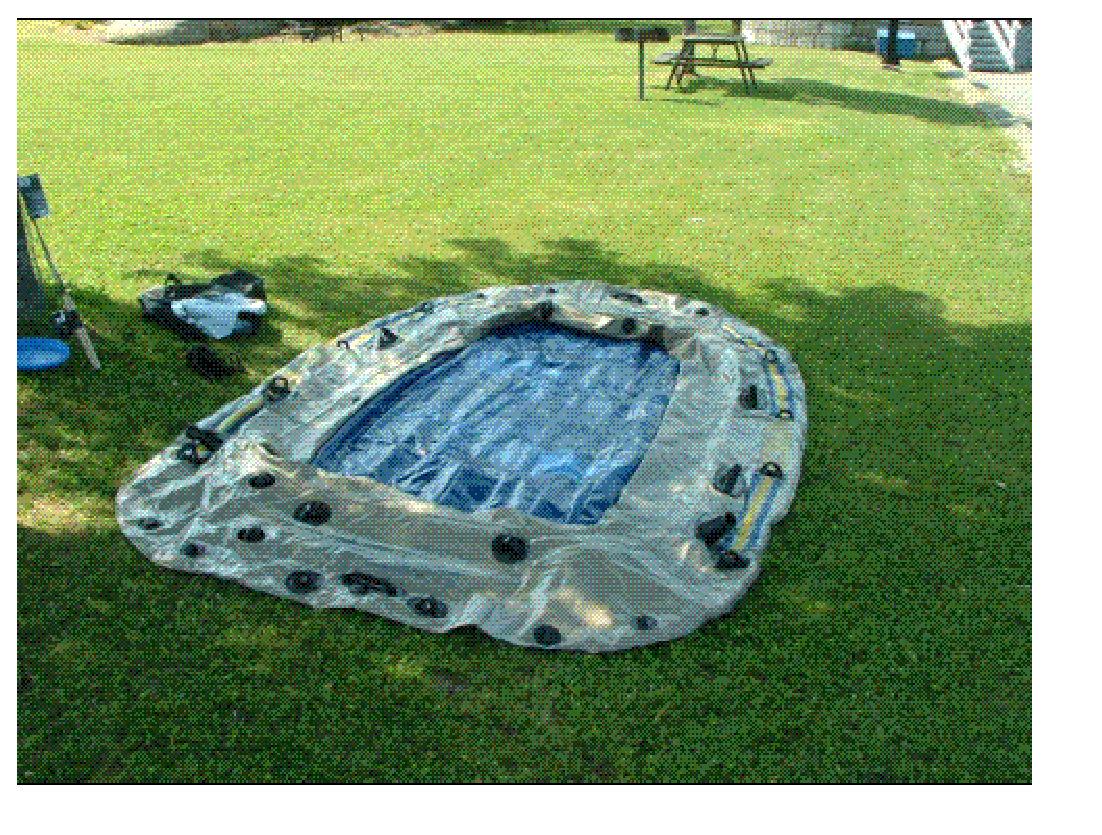
\epsfig{file=fig1.eps,width=3.5in}
Which one of the following is missing in it?
 
 
\noindent{\textbf{\large{
A.}}}
A truck
 
 
\noindent{\textbf{\large{
B.}}}
An air-boat
 
 
\noindent{\textbf{\large{
C.}}}
An airplane
 
 
\noindent{\textbf{\large{
D.}}}
A frisbee
 
 
\noindent{\textbf{\large{
E.}}}
A table
 
 
\noindent{\textbf{\large{
F.}}}
  Not any of aboves.
 
 
\noindent\vspace{0.05in}{\textbf{\Large{Auto-answer:}}}
 
 
\noindent{\textbf{\large{
A.}}}
A truck
 
 
\noindent{\textbf{\large{
C.}}}
An airplane
 
 
\noindent\vspace{0.05in}{\textbf{\Large{End of auto-answer.}}}
 
 
 
\vspace{0.3in}
   
   
\noindent{\textbf{\Large{Total numbers: }}}
   
   
\noindent\begin{tabular}{|l|l|l|l|l|l|l|}
 \hline
Inputs & Calculates & Choices & Layers & Matches & Answer & Solution \\ \hline
           0 & 
           0 & 
           6
  simple  
  & 
           6 & 
           0 & 
  yes & 
  no 
  \\ \hline
 \end{tabular}
   
   
   
   
\noindent\vspace{0.1in}{\textbf{\Large{Calculated values:}}}
   
   
   
   
\noindent\vspace{0.1in}\hspace{-0.08in} {\textbf{\Large{All inputs: }}}
   
   
  
\vspace{0.2in}
  
{\textbf{\Large{Question
32.1.6 
 (          6,          6,         21)
}}}
  
  
 
An object is subjected to an external net force $\mathbf{f}=(
50.0,  % 
5.0,
-3000.0  )N$. Its mass is known as
$m= % 
54.0 kg$. Please calculate its accelaration.
 
 
 
 
\noindent\vspace{0.05in}{\textbf{\Large{Answer:}}}
 
 

We will use the Newton's Second Law:
 
\[
\mathbf{f}=m\mathbf{a}.
\]
 
Since $\mathbf{f}=( % 
50.0,  % 
5.0,  % 
-3000.0 )N$
and $m= % 
54.0 kg$, bring them into the above equation, then we get
 
\begin{eqnarray*}
\mathbf{a}&=&\frac{\mathbf{f}}m  \\
&=&\frac{(
50.0 ,
5.0 ,
-3000.0 )N
}{ % 
54.0 kg}  \\
&=&(
.92593 ,
9.2593 \times 10^{-2},
-55.556
)ms^{-2} \\
&=&(
12000. ,
1200.0 ,
-720000.
)km/h^2.
\end{eqnarray*}
 
 
 
\noindent\vspace{0.05in}{\textbf{\Large{End of Answer.}}}
 
 

 
 
 
\noindent\vspace{0.1in}{\textbf{\Large{Solution: }}}
 
 

We will use the Newton's Second Law:
 
\[
\mathbf{f}=m\mathbf{a}.
\]
 
Since $\mathbf{f}=( % 
50.0,  % 
5.0,  % 
-3000.0 )N$
and $m= % 
54.0 kg$, bring them into the above equation, then we get
 
\begin{eqnarray*}
\mathbf{a}&=&\frac{\mathbf{f}}m  \\
&=&\frac{(
50.0 ,
5.0 ,
-3000.0 )N
}{ % 
54.0 kg}  \\
&=&(
.92593 ,
9.2593 \times 10^{-2},
-55.556
)ms^{-2} \\
&=&(
12000. ,
1200.0 ,
-720000.
)km/h^2.
\end{eqnarray*}
 
 
 
\noindent\vspace{0.1in}{\textbf{\Large{End of Solution.}}}
 
 

 
\vspace{0.3in}
   
   
\noindent{\textbf{\Large{Total numbers: }}}
   
   
\noindent\begin{tabular}{|l|l|l|l|l|l|l|}
 \hline
Inputs & Calculates & Choices & Layers & Matches & Answer & Solution \\ \hline
           4 & 
           6 & 
           0
  & 
           0 & 
           0 & 
  yes & 
  yes 
  \\ \hline
 \end{tabular}
   
   
   
   
\noindent\vspace{0.1in}{\textbf{\Large{Calculated values:}}}
   
   
  
  
\noindent\begin{tabular}{|l|l|l|l|}
\hline
 Sequential & Type & Accuracy & Calculated \\ 
\hline
 
 
  Calculated $           1$ & real & $           5 $ & 
 $ .92593 $ 
 \\  \hline  
 
 
  Calculated $           2$ & real & $           5 $ & 
 $ 9.2593 \times 10^{-2} $ 
 \\  \hline  
 
 
  Calculated $           3$ & real & $           5 $ & 
 $ -55.556 $ 
 \\  \hline  
 
 
  Calculated $           4$ & real & $           5 $ & 
 $ 12000. $ 
 \\  \hline  
 
 
  Calculated $           5$ & real & $           5 $ & 
 $ 1200.0 $ 
 \\  \hline  
 
 
  Calculated $           6$ & real & $           5 $ & 
 $ -720000. $ 
 \\  \hline  
 \end{tabular}
   
   
   
   
\noindent\vspace{0.1in}\hspace{-0.08in} {\textbf{\Large{All inputs: }}}
   
   
  
  
\noindent\begin{tabular}{|l|l|l|l|l|}
\hline
 Sequential & Type & Accuracy & Three inputs & Generated \\ 
\hline
 
 
  INPUT $           1$ & real & $          -1 $ & $
 20.0
  $ & \\
  & & &  $
 101.0
  $ & \\
  & & &  $
 10.0
 $ & $ 50.0 $ 
 \\  \hline  
 
 
  INPUT $           2$ & real & $          -1 $ & $
 2.0
  $ & \\
  & & &  $
 10.1
  $ & \\
  & & &  $
 1.0
 $ & $ 5.0 $ 
 \\  \hline  
 
 
  INPUT $           3$ & real & $          -1 $ & $
 -2000.0
  $ & \\
  & & &  $
 -10001.0
  $ & \\
  & & &  $
 -1000.0
 $ & $ -3000.0 $ 
 \\  \hline  
 \end{tabular}
   
   
  
  
\noindent\begin{tabular}{|l|l|l|l|l|}
\hline
 Sequential & Type & Accuracy & Three inputs & Generated \\ 
\hline
 
 
  INPUT $           4$ & real & $          -1 $ & $
 50.0
  $ & \\
  & & &  $
 60.1
  $ & \\
  & & &  $
 2.0
 $ & $ 54.0 $ 
 \\  \hline  
 \end{tabular}
   
   
   
   
\vspace{0.3in}
{\textbf{\LARGE{You have done all the above? A very good beginning, please go ahead.}}}
More constants the
Mass of electron
$m_e$$ =
9.109390 \times 10^{-31} $
kg
,
Universal gas constant
$R$$ =
8.315 $
J/(mol$\cdot $K)
,
$e$$ =
1.60217733 \times 10^{-19} $
C
, and
$m_p$$ =
1.6726231 \times 10^{-27} $
kg
%
may be very helpful.
\vspace{0.3in}
   
   
  
\vspace{0.2in}
  
{\textbf{\Large{QUESTION
32.2 
 (          5,          5,          5)
}}}
  
  
If any one of the following statements is correct, please fill the box ahead of it with $T$ .
If wrong, fill with $F$.
 
\noindent\begin{tabular}{|l|l|}\hline Your&\hspace{.2in} \\ answer&\hspace{.2in} \\ \hline \end{tabular}
1. $ % 
5$ is an  % 
odd number.
 
\noindent\begin{tabular}{|l|l|}\hline Your&\hspace{.2in} \\ answer&\hspace{.2in} \\ \hline \end{tabular}
2.  % 
Kingston is in  % 
Ontario province.
 
\noindent\begin{tabular}{|l|l|}\hline Your&\hspace{.2in} \\ answer&\hspace{.2in} \\ \hline \end{tabular}
3.  % 
$\mathbf{F}=m\mathbf{a}$ is a mathmatical form of
the Newton's Second Law.
 
 
 
\noindent\vspace{0.05in}{\textbf{\Large{Answer:}}}
 
 

 
\noindent\begin{tabular}{|l|l|}\hline The correct & \\
          answer &  % 
$T$ \\ \hline \end{tabular}
1. $ % 
5$ is an  % 
odd number.
 
\noindent\begin{tabular}{|l|l|}\hline The correct & \\
          answer &  % 
$T$ \\ \hline \end{tabular}
2.  % 
Kingston is in  % 
Ontario province.
 
\noindent\begin{tabular}{|l|l|}\hline The correct & \\
          answer &  % 
$T$ \\ \hline \end{tabular}
3.  % 
$\mathbf{F}=m\mathbf{a}$ is a mathmatical form of  % 
the Newton's Second Law.
 
 
 
\noindent\vspace{0.05in}{\textbf{\Large{End of Answer.}}}
 
 

 
\vspace{0.3in}
   
   
\noindent{\textbf{\Large{Total numbers: }}}
   
   
\noindent\begin{tabular}{|l|l|l|l|l|l|l|}
 \hline
Inputs & Calculates & Choices & Layers & Matches & Answer & Solution \\ \hline
           6 & 
           3 & 
           0
  & 
           0 & 
           0 & 
  yes & 
  no 
  \\ \hline
 \end{tabular}
   
   
   
   
\noindent\vspace{0.1in}{\textbf{\Large{Calculated values:}}}
   
   
  
  
\noindent\begin{tabular}{|l|l|l|l|}
\hline
 Sequential & Type & Accuracy & Calculated \\ 
\hline
 
 
  Calculated $           1$ & string & $           1 $ ( $          2 $ strings)
 : 
 & $T$
 \\  \hline  
 
 
  Calculated $           2$ & string & $           1 $ ( $          2 $ strings)
 : 
 & $T$
 \\  \hline  
 
 
  Calculated $           3$ & string & $           1 $ ( $          2 $ strings)
 : 
 & $T$
 \\  \hline  
 \end{tabular}
   
   
   
   
\noindent\vspace{0.1in}\hspace{-0.08in} {\textbf{\Large{All inputs: }}}
   
   
  
  
\noindent\begin{tabular}{|l|l|l|l|l|}
\hline
 Sequential & Type & Accuracy & Three inputs & Generated \\ 
\hline
 
 
  INPUT $           1$ & integer &  & $
 1
 , 
 100
 , 
 1
 $ & $ 5 $ 
 \\  \hline  
 
 
  INPUT $           2$ & string & & 
 even & 
  \\
  & & & 
 odd & 
  $ <-- $ 
 \\  \hline  
 
 
  INPUT $           3$ & string & & 
 Toronto & 
  \\
  & & & 
 Kingston & 
  $ <-- $ 
  \\
  & & & 
 Montreal & 
  \\
  & & & 
 Hull & 
 \\  \hline  
 \end{tabular}
   
   
  
  
\noindent\begin{tabular}{|l|l|l|l|l|}
\hline
 Sequential & Type & Accuracy & Three inputs & Generated \\ 
\hline
 
 
  INPUT $           4$ & string & & 
 Ontario & 
  $ <-- $ 
  \\
  & & & 
 Quebec & 
 \\  \hline  
 
 
  INPUT $           5$ & string & & 
 $\mathbf{F}=m\mathbf{a}$ & 
  $ <-- $ 
  \\
  & & & 
 $\left| \mathbf{F}\right| =Gm_1m_2r^{-2}$ & 
 \\  \hline  
 
 
  INPUT $           6$ & string & & 
 the Newton's Second Law & 
  $ <-- $ 
  \\
  & & & 
 Newton's Law of Universal Gravitation & 
 \\  \hline  
 \end{tabular}
   
   
  
\vspace{0.2in}
  
{\textbf{\Large{QUESTION
32.3 
 (          4,          4,          4)
}}}
  
  
Considering case-insensitivity, please match the following same strings.
  
  
\begin{tabular}{|l|l|l|}
 \hline
 Column Left & Column Right  & Your choinces \\ 
 \hline
{\textbf{\large{
A.}}}
yjh
  & 
eR
 & 
 \\ 
 \hline
{\textbf{\large{
B.}}}
C
  & 
b
 & 
 \\ 
 \hline
{\textbf{\large{
C.}}}
er
  & 
YJH
 & 
 \\ 
 \hline
{\textbf{\large{
D.}}}
Er
  & 
ER
 & 
 \\ 
 \hline
{\textbf{\large{
E.}}}
B
  & 
c
 & 
 \\ 
 \hline
 \end{tabular}
  
  
 
 
\noindent\vspace{0.05in}{\textbf{\Large{Auto-answer:}}}
  
  
\begin{tabular}{|l|l|l|}
 \hline
 Column Left & Column Right  & Answers       \\ 
 \hline
{\textbf{\large{
A.}}}
yjh
  & 
eR
 & 
{\textbf{\large{
C.}}}
, 
{\textbf{\large{
D.}}}
 \\ 
 \hline
{\textbf{\large{
B.}}}
C
  & 
b
 & 
{\textbf{\large{
E.}}}
 \\ 
 \hline
{\textbf{\large{
C.}}}
er
  & 
YJH
 & 
{\textbf{\large{
A.}}}
 \\ 
 \hline
{\textbf{\large{
D.}}}
Er
  & 
ER
 & 
{\textbf{\large{
C.}}}
, 
{\textbf{\large{
D.}}}
 \\ 
 \hline
{\textbf{\large{
E.}}}
B
  & 
c
 & 
{\textbf{\large{
B.}}}
 \\ 
 \hline
 \end{tabular}
  
  
 
 
\noindent\vspace{0.05in}{\textbf{\Large{End of auto-answer.}}}
 
 
 
   
   
\noindent{\textbf{\Large{Total numbers: }}}
   
   
\noindent\begin{tabular}{|l|l|l|l|l|l|l|}
 \hline
Inputs & Calculates & Choices & Layers & Matches & Answer & Solution \\ \hline
           2 & 
           1 & 
           0
  & 
          16 & 
           5 & 
  yes & 
  no 
  \\ \hline
 \end{tabular}
   
   
   
   
\noindent\vspace{0.1in}{\textbf{\Large{Calculated values:}}}
   
   
  
  
\noindent\begin{tabular}{|l|l|l|l|}
\hline
 Sequential & Type & Accuracy & Calculated \\ 
\hline
 
 
  Calculated $           1$ & integer &  & 
  $ 3 $ 
 \\  \hline  
 \end{tabular}
   
   
   
   
\noindent\vspace{0.1in}\hspace{-0.08in} {\textbf{\Large{All inputs: }}}
   
   
  
  
\noindent\begin{tabular}{|l|l|l|l|l|}
\hline
 Sequential & Type & Accuracy & Three inputs & Generated \\ 
\hline
 
 
  INPUT $           1$ & integer &  & $
 2
 , 
 8
 , 
 2
 $ & $ 6 $ 
 \\  \hline  
 
 
  INPUT $           2$ & integer &  & $
 2
 , 
 3
 , 
 2
 $ & $ 2 $ 
 \\  \hline  
 \end{tabular}
   
   
  
\vspace{0.2in}
  
{\textbf{\Large{QUESTION
32.4 
 (          2,          2,          2)
}}}
  
  
 
An object is subjected to an external net force $\mathbf{f}=(
20.000 ,
10.0000,
-9000.0  )N$. Its mass is known as
$m= % 
58.0000  kg$. Please choose the correct accelaration
from the following choices.
 
 
 
\noindent{\textbf{\large{
A.}}}
The accelaration is
$(
.99840ms^{-2},
2234.5km/h^2,
-155.17ms^{-2}
).
$
 
 
\noindent{\textbf{\large{
B.}}}
The accelaration is
$(
.34483ms^{-2},
2234.5km/h^2,
-405.11ms^{-2}
).
$
 
 
\noindent{\textbf{\large{
C.}}}
The accelaration is
$(
.34483ms^{-2},
-10755.km/h^2,
-155.17ms^{-2}
).
$
 
 
\noindent{\textbf{\large{
D.}}}
The accelaration is
$(
.99840ms^{-2},
2234.5km/h^2,
-405.11ms^{-2}
).
$
 
 
\noindent{\textbf{\large{
E.}}}
The accelaration is
$(
.34483ms^{-2},
2234.5km/h^2,
-155.17ms^{-2}
).
$
 
 
\noindent{\textbf{\large{
F.}}}
The accelaration is
$(
.99840ms^{-2},
-10755.km/h^2,
-155.17ms^{-2}
).
$
 
 
\noindent{\textbf{\large{
G.}}}
 None of these.
 
 
\noindent\vspace{0.05in}{\textbf{\Large{Auto-answer:}}}
 
 
\noindent{\textbf{\large{
E.}}}
The accelaration is
$(
.34483ms^{-2},
2234.5km/h^2,
-155.17ms^{-2}
).
$
 
 
\noindent\vspace{0.05in}{\textbf{\Large{End of auto-answer.}}}
 
 
 
 
 
 
\noindent\vspace{0.1in}{\textbf{\Large{Solution: }}}
 
 

We will use the Newton's Second Law:
 
\[
\mathbf{f}=m\mathbf{a}.
\]
 
Since $\mathbf{f}=( % 
20.000,  % 
10.0000,  % 
-9000.0 )N$
and $m= % 
58.0000kg$, bring them into the above equation, then we get
 
\begin{eqnarray*}
\mathbf{a}&=&\frac{\mathbf{f}}m  \\
&=&\frac{(
20.000 ,
10.0000 ,
-9000.0 )N
}{ % 
58.0000 kg}  \\
&=&(
.34483 ,
.17241,
-155.17
)ms^{-2} \\
&=&(
4469.0 ,
2234.5 ,
-2.0110 \times 10^{6}
)km/h^2.
\end{eqnarray*}
 
 
 
\noindent\vspace{0.1in}{\textbf{\Large{End of Solution.}}}
 
 

 
\vspace{0.3in}
   
   
\noindent{\textbf{\Large{Total numbers: }}}
   
   
\noindent\begin{tabular}{|l|l|l|l|l|l|l|}
 \hline
Inputs & Calculates & Choices & Layers & Matches & Answer & Solution \\ \hline
           4 & 
           6 & 
           7
  & 
           3 & 
           0 & 
  yes & 
  yes 
  \\ \hline
 \end{tabular}
   
   
   
   
\noindent\vspace{0.1in}{\textbf{\Large{Calculated values:}}}
   
   
  
  
\noindent\begin{tabular}{|l|l|l|l|}
\hline
 Sequential & Type & Accuracy & Calculated \\ 
\hline
 
 
  Calculated $           1$ & real & $           5 $ & 
 $ .34483 $ 
 \\  \hline  
 
 
  Calculated $           2$ & real & $           5 $ & 
 $ .17241 $ 
 \\  \hline  
 
 
  Calculated $           3$ & real & $           5 $ & 
 $ -155.17 $ 
 \\  \hline  
 
 
  Calculated $           4$ & real & $           5 $ & 
 $ 4469.0 $ 
 \\  \hline  
 
 
  Calculated $           5$ & real & $           5 $ & 
 $ 2234.5 $ 
 \\  \hline  
 
 
  Calculated $           6$ & real & $           5 $ & 
 $ -2.0110 \times 10^{6} $ 
 \\  \hline  
 \end{tabular}
   
   
   
   
\noindent\vspace{0.1in}\hspace{-0.08in} {\textbf{\Large{All inputs: }}}
   
   
  
  
\noindent\begin{tabular}{|l|l|l|l|l|}
\hline
 Sequential & Type & Accuracy & Three inputs & Generated \\ 
\hline
 
 
  INPUT $           1$ & real & $          -3 $ & $
 20.000
  $ & \\
  & & &  $
 101.000
  $ & \\
  & & &  $
 10.000
 $ & $ 20.000 $ 
 \\  \hline  
 
 
  INPUT $           2$ & real & $          -4 $ & $
 2.0000
  $ & \\
  & & &  $
 10.1000
  $ & \\
  & & &  $
 1.0000
 $ & $ 10.0000 $ 
 \\  \hline  
 
 
  INPUT $           3$ & real & $          -1 $ & $
 -2000.0
  $ & \\
  & & &  $
 -10001.0
  $ & \\
  & & &  $
 -1000.0
 $ & $ -9000.0 $ 
 \\  \hline  
 \end{tabular}
   
   
  
  
\noindent\begin{tabular}{|l|l|l|l|l|}
\hline
 Sequential & Type & Accuracy & Three inputs & Generated \\ 
\hline
 
 
  INPUT $           4$ & real & $          -4 $ & $
 50.0000
  $ & \\
  & & &  $
 60.1000
  $ & \\
  & & &  $
 2.0000
 $ & $ 58.0000 $ 
 \\  \hline  
 \end{tabular}
   
   
  
\vspace{0.2in}
  
{\textbf{\Large{QUESTION
32.5 
 (          3,          3,          3)
}}}
  
  
Please choose the correct one from the following statements:
 
 
\noindent{\textbf{\large{
A.}}}
Canada has  %
10 provinces and  %
3 territories.
 
 
\noindent{\textbf{\large{
B.}}}
Canada has  %
37 provinces and  %
37 territories.
 
 
\noindent{\textbf{\large{
C.}}}
Canada has  %
34 provinces and  %
39 territories.
 
 
\noindent{\textbf{\large{
D.}}}
Canada has  %
36 provinces and  %
35 territories.
 
 
\noindent{\textbf{\large{
E.}}}
Canada has  %
35 provinces and  %
34 territories.
 
 
\noindent{\textbf{\large{
F.}}}
 None of above.
 
 
\noindent\vspace{0.05in}{\textbf{\Large{Auto-answer:}}}
 
 
\noindent{\textbf{\large{
A.}}}
Canada has  %
10 provinces and  %
3 territories.
 
 
\noindent\vspace{0.05in}{\textbf{\Large{End of auto-answer.}}}
 
 
   
   
\noindent{\textbf{\Large{Total numbers: }}}
   
   
\noindent\begin{tabular}{|l|l|l|l|l|l|l|}
 \hline
Inputs & Calculates & Choices & Layers & Matches & Answer & Solution \\ \hline
           0 & 
          20 & 
           6
  simple  
  & 
           6 & 
           0 & 
  yes & 
  no 
  \\ \hline
 \end{tabular}
   
   
   
   
\noindent\vspace{0.1in}{\textbf{\Large{Calculated values:}}}
   
   
  
  
\noindent\begin{tabular}{|l|l|l|l|}
\hline
 Sequential & Type & Accuracy & Calculated \\ 
\hline
 
 
  Calculated $           1$ & integer &  & 
  $ 10 $ 
 \\  \hline  
 
 
  Calculated $           2$ & integer &  & 
  $ 3 $ 
 \\  \hline  
 
 
  Calculated $           3$ & integer &  & 
  $ 23 $ 
 \\  \hline  
 
 
  Calculated $           4$ & integer &  & 
  $ 24 $ 
 \\  \hline  
 
 
  Calculated $           5$ & integer &  & 
  $ 25 $ 
 \\  \hline  
 
 
  Calculated $           6$ & integer &  & 
  $ 26 $ 
 \\  \hline  
 
 
  Calculated $           7$ & integer &  & 
  $ 27 $ 
 \\  \hline  
 
 
  Calculated $           8$ & integer &  & 
  $ 28 $ 
 \\  \hline  
 
 
  Calculated $           9$ & integer &  & 
  $ 29 $ 
 \\  \hline  
 
 
  Calculated $          10$ & integer &  & 
  $ 30 $ 
 \\  \hline  
 \end{tabular}
   
   
  
  
\noindent\begin{tabular}{|l|l|l|l|}
\hline
 Sequential & Type & Accuracy & Calculated \\ 
\hline
 
 
  Calculated $          11$ & integer &  & 
  $ 31 $ 
 \\  \hline  
 
 
  Calculated $          12$ & integer &  & 
  $ 32 $ 
 \\  \hline  
 
 
  Calculated $          13$ & integer &  & 
  $ 33 $ 
 \\  \hline  
 
 
  Calculated $          14$ & integer &  & 
  $ 34 $ 
 \\  \hline  
 
 
  Calculated $          15$ & integer &  & 
  $ 35 $ 
 \\  \hline  
 
 
  Calculated $          16$ & integer &  & 
  $ 36 $ 
 \\  \hline  
 
 
  Calculated $          17$ & integer &  & 
  $ 37 $ 
 \\  \hline  
 
 
  Calculated $          18$ & integer &  & 
  $ 38 $ 
 \\  \hline  
 
 
  Calculated $          19$ & integer &  & 
  $ 39 $ 
 \\  \hline  
 
 
  Calculated $          20$ & integer &  & 
  $ 40 $ 
 \\  \hline  
 \end{tabular}
   
   
   
   
\noindent\vspace{0.1in}\hspace{-0.08in} {\textbf{\Large{All inputs: }}}
   
   
  
\vspace{0.2in}
  
{\textbf{\Large{QUESTION
32.6 
 (          1,          1,          1)
}}}
  
  


\noindent\vspace{0.05in}{\textbf{\Large{Abstract:}}}
This is a simple Newton's Second Law calculation multi-choice problem.  
\noindent\vspace{0.05in}{\textbf{\Large{end of abstract.}}}


 
 
An object is subjected to an external net force $\mathbf{f}=
(40.0 , 8.0 , -6000.0) N$.
Its mass is known as $m= % 
50.0000 kg$. Please choose the
correct accelaration from the following choices.
 
 
 
\noindent{\textbf{\large{
A.}}}
The accelaration is $  %
(
2.65,
.16,
-120.00)
ms^{-2} $.
 
 
\noindent{\textbf{\large{
B.}}}
The accelaration is $  %
(
.800,
-.64,
-120.00)
ms^{-2} $.
 
 
\noindent{\textbf{\large{
C.}}}
The accelaration is $  %
(
2.65,
-.64,
-120.00)
ms^{-2} $.
 
 
\noindent{\textbf{\large{
D.}}}
The accelaration is $  %
(
2.65,
.16,
-347.33)
ms^{-2} $.
 
 
\noindent{\textbf{\large{
E.}}}
The accelaration is $  %
(
2.65,
-.64,
-347.33)
ms^{-2} $.
 
 
\noindent{\textbf{\large{
F.}}}
The accelaration is $  %
(
.800,
.16,
-120.00)
ms^{-2} $.
 
 
\noindent{\textbf{\large{
G.}}}
The accelaration is $  %
(
.800,
-.64,
-347.33)
ms^{-2} $.
 
 
\noindent{\textbf{\large{
H.}}}
The accelaration is $  %
(
.800,
.16,
-347.33)
ms^{-2} $.
 
 
\noindent\vspace{0.05in}{\textbf{\Large{Auto-answer:}}}
 
 
\noindent{\textbf{\large{
F.}}}
The accelaration is $  %
(
.800,
.16,
-120.00)
ms^{-2} $.
 
 
\noindent\vspace{0.05in}{\textbf{\Large{End of auto-answer.}}}
 
 
 
 
 
\noindent\vspace{0.05in}{\textbf{\Large{Answer:}}}
 
 

The correct answer from the choices is


\noindent{\textbf{\large{
F.}}}
The accelaration is $  %
(
.800,
.16,
-120.00)
ms^{-2} $.
 
 
 
\noindent\vspace{0.05in}{\textbf{\Large{End of Answer.}}}
 
 

 
 
 
\noindent\vspace{0.1in}{\textbf{\Large{Solution: }}}
 
 

We will use the Newton's Second Law:
 
\[
\mathbf{f}=m\mathbf{a}.
\]
 
Since $\mathbf{f}= % 
(40.0 , 8.0 , -6000.0) N$
and $m= % 
50.0000kg$, bring them into the above equation, then we get
 
\begin{eqnarray*}
\mathbf{a}&=&\frac{\mathbf{f}}m  \\
&=&\frac{ % 
(40.0 , 8.0 , -6000.0) N}{ % 
50.0000kg}  \\
&=& % 
(.800 , .16 , -120.00) ms^{-2}
\end{eqnarray*}
 
 
 
\noindent\vspace{0.1in}{\textbf{\Large{End of Solution.}}}
 
 

 
\vspace{0.3in}
   
   
\noindent{\textbf{\Large{Total numbers: }}}
   
   
\noindent\begin{tabular}{|l|l|l|l|l|l|l|}
 \hline
Inputs & Calculates & Choices & Layers & Matches & Answer & Solution \\ \hline
           2 & 
           1 & 
           8
  & 
           3 & 
           0 & 
  yes & 
  yes 
  \\ \hline
 \end{tabular}
   
   
   
   
\noindent\vspace{0.1in}{\textbf{\Large{Calculated values:}}}
   
   
  
  
\noindent\begin{tabular}{|l|l|l|l|}
\hline
 Sequential & Type & Accuracy & Calculated \\ 
\hline
 
 
  Calculated $           1$ & vector &  
  $           3 $ 
 &  $ .800 $ 
 \\    
  & & 
  $           2 $ 
 &  $ .16 $ 
 \\    
  & & 
  $           5 $ 
 &  $ -120.00 $ 
 \\  \hline  
 \end{tabular}
   
   
   
   
\noindent\vspace{0.1in}\hspace{-0.08in} {\textbf{\Large{All inputs: }}}
   
   
  
  
\noindent\begin{tabular}{|l|l|l|l|l|}
\hline
 Sequential & Type & Accuracy & Three inputs & Generated \\ 
\hline
 
 
  INPUT $           1$ & vector & $          -1 $ & $
20.0
  $ & \\
  & & & $
101.0
  $ & \\
  & & & $
10.0
$ & $ 40.0 $ 
  \\
  & & $          -1 $ & $
2.0
  $ & \\
  & & & $
10.1
  $ & \\
  & & & $
1.0
$ & $ 8.0 $ 
  \\
  & & $          -1 $ & $
-2000.0
  $ & \\
  & & & $
-10001.0
  $ & \\
  & & & $
-1000.0
$ & $ -6000.0 $ 
 \\  \hline  
 
 
  INPUT $           2$ & real & $          -4 $ & $
 50.0000
  $ & \\
  & & &  $
 60.1000
  $ & \\
  & & &  $
 2.0000
 $ & $ 50.0000 $ 
 \\  \hline  
 \end{tabular}
   
   
   
   
\vspace{0.3in}
{\textbf{\LARGE{You have done all the above? Excellent! Not much left, please continue.}}}
\vspace{0.3in}
   
   
  
\vspace{0.2in}
  
{\textbf{\Large{QUESTION
32.7 
 (          8,         15,         60)
}}}
  
  
 
$ \left( \begin{array}{ccccccccc}
           7 & 
           4 & 
           4 & 
           7 \\ 
           6 & 
           4 & 
           5 & 
           7 \\ 
           5 & 
           6 & 
           6 & 
           5
\end{array}\right) \times
\left( \begin{array}{c}
           2 \\ 
           2 \\ 
           2 \\ 
           2
\end{array}\right) $ =?
 
 
$  % 
 \left( \begin{array}
 {
 c
 c
 }
                    \Xi & 
 \eta \\ 
 \Upsilon & 
 \Lambda \\ 
 \delta & 
 \delta \\ 
 \rho & 
 \sigma
 \end{array} \right)
 \left( \begin{array}
 {
 c
 }
 \beta \\ 
 \beta
 \end{array} \right)
$ =?
 
 
 
\noindent\vspace{0.05in}{\textbf{\Large{Answer:}}}
 
 

 
$\left( \begin{array}{ccccccccccccccc}
           7 & 
           4 & 
           4 & 
           7 \\ 
           6 & 
           4 & 
           5 & 
           7 \\ 
           5 & 
           6 & 
           6 & 
           5
\end{array}\right) \times
\left( \begin{array}{c}
           2 \\ 
           2 \\ 
           2 \\ 
           2
\end{array}\right)  =
\left( \begin{array}{c}
          44 \\ 
          44 \\ 
          44
\end{array}\right)  $
 
$  % 
 \left( \begin{array}
 {
 c
 c
 }
                    \Xi & 
 \eta \\ 
 \Upsilon & 
 \Lambda \\ 
 \delta & 
 \delta \\ 
 \rho & 
 \sigma
 \end{array} \right)
 \left( \begin{array}
 {
 c
 }
 \beta \\ 
 \beta
 \end{array} \right)
=
  \left( \begin{array}
 {
 c
 }
                    \Xi \times  \beta   +  \eta \times  \beta \\ 
 \Upsilon \times  \beta   +  \Lambda \times  \beta \\ 
 \delta \times  \beta   +  \delta \times  \beta \\ 
 \rho \times  \beta   +  \sigma \times  \beta
 \end{array} \right)
$
 
 
 
\noindent\vspace{0.05in}{\textbf{\Large{End of Answer.}}}
 
 

 
 
 
\noindent\vspace{0.1in}{\textbf{\Large{Solution: }}}
 
 

 
 
\noindent\vspace{0.1in}{\textbf{\Large{End of Solution.}}}
 
 

 
\vspace{0.3in}
   
   
\noindent{\textbf{\Large{Total numbers: }}}
   
   
\noindent\begin{tabular}{|l|l|l|l|l|l|l|}
 \hline
Inputs & Calculates & Choices & Layers & Matches & Answer & Solution \\ \hline
           4 & 
           2 & 
           0
  & 
           0 & 
           0 & 
  yes & 
  yes 
  \\ \hline
 \end{tabular}
   
   
   
   
\noindent\vspace{0.1in}{\textbf{\Large{Calculated values:}}}
   
   
  
  
\noindent\begin{tabular}{|l|l|l|l|}
\hline
 Sequential & Type & Accuracy & Calculated \\ 
\hline
 
 
  Calculated $           1$ & i-matrix &  & 
 (size:           3 by           1)
 \\  \hline  
 \end{tabular}
   
   
$\begin{array}{
 c
 }
          44 \\ 
          44 \\ 
          44
 \end{array}  $ 
  
  
\noindent\begin{tabular}{|l|l|l|l|}
\hline
 Sequential & Type & Accuracy & Calculated \\ 
\hline
 
 
  Calculated $           2$ & s-matrix & & 
 (size:           4 by           1)
 \\  \hline  
 \end{tabular}
   
   
 $   \left( \begin{array}
 {
 c
 }
                    \Xi \times  \beta   +  \eta \times  \beta \\ 
 \Upsilon \times  \beta   +  \Lambda \times  \beta \\ 
 \delta \times  \beta   +  \delta \times  \beta \\ 
 \rho \times  \beta   +  \sigma \times  \beta
 \end{array} \right) $ 
   
   
\noindent\vspace{0.1in}\hspace{-0.08in} {\textbf{\Large{All inputs: }}}
   
   
  
  
\noindent\begin{tabular}{|l|l|l|l|l|}
\hline
 Sequential & Type & Accuracy & Three inputs & Generated \\ 
\hline
 
 
  INPUT $           1$ & i-matrix &  & $
 4
 , 
 7
 , 
 1
 $ & (size:           3 by           4)
 \\  \hline  
 \end{tabular}
   
   
 $\begin{array}{
 c
 c
 c
 c
 }
           7 & 
           4 & 
           4 & 
           7 \\ 
           6 & 
           4 & 
           5 & 
           7 \\ 
           5 & 
           6 & 
           6 & 
           5
\end{array}  $ 
  
  
\noindent\begin{tabular}{|l|l|l|l|l|}
\hline
 Sequential & Type & Accuracy & Three inputs & Generated \\ 
\hline
 
 
  INPUT $           2$ & i-matrix &  & $
 2
 , 
 2
 , 
 1
 $ & (size:           4 by           1)
 \\  \hline  
 \end{tabular}
   
   
 $\begin{array}{
 c
 }
           2 \\ 
           2 \\ 
           2 \\ 
           2
\end{array}  $ 
  
  
\noindent\begin{tabular}{|l|l|l|l|l|}
\hline
 Sequential & Type & Accuracy & Three inputs & Generated \\ 
\hline
 
 
  INPUT $           3$ & s-matrix & & 
 $  \alpha $ & 
  \\
  & & & 
 $  \beta $ & 
  \\
  & & & 
 $  \gamma $ & 
  \\
  & & & 
 $  \delta $ & 
  \\
  & & & 
 $  \epsilon $ & 
  \\
  & & & 
 $  \varepsilon $ & 
  \\
  & & & 
 $                     \zeta $ & 
  \\
  & & & 
 $  \eta $ & 
  \\
  & & & 
 $  \rho $ & 
  \\
  & & & 
 $  \sigma $ & 
  \\
  & & & 
 $  \Gamma $ & 
  \\
  & & & 
 $  \Delta $ & 
  \\
  & & & 
 $  \Theta $ & 
  \\
  & & & 
 $  \Lambda $ & 
  \\
  & & & 
 $                     \Xi $ & 
  \\
  & & & 
 $  \Upsilon $ & 
  \\
  & & & 
 $  \Phi $ & 
  \\
  & & & 
 $  \Psi $ & 
  \\
  & & & 
 $  \Omega $ & 
  (size:           4 by           2)
 \\  \hline  
 \end{tabular}
   
   
 $  \left( \begin{array}
 {
 c
 c
 }
                    \Xi & 
 \eta \\ 
 \Upsilon & 
 \Lambda \\ 
 \delta & 
 \delta \\ 
 \rho & 
 \sigma
 \end{array} \right) $ 
  
  
\noindent\begin{tabular}{|l|l|l|l|l|}
\hline
 Sequential & Type & Accuracy & Three inputs & Generated \\ 
\hline
 
 
  INPUT $           4$ & s-matrix & & 
 $  \beta $ & 
  \\
  & & & 
 $  \gamma $ & 
  (size:           2 by           1)
 \\  \hline  
 \end{tabular}
   
   
 $  \left( \begin{array}
 {
 c
 }
 \beta \\ 
 \beta
 \end{array} \right) $ 
  
\vspace{0.2in}
  
{\textbf{\Large{QUESTION
32.8 
 (          7,         14,         50)
}}}
  
  
 
An object is subjected to an external net force $\mathbf{f}=
(70.0 , 6.0 , -5000.0) N$.
Its mass is known as $m= % 
58.0 kg$.
Please choose the correct accelaration from the following choices.
 
 
\noindent{\textbf{\large{
A.}}}
  The accelaration is $  %
(
1.21,
.10,
329.96)
ms^{-2} $.
 
 
\noindent{\textbf{\large{
B.}}}
  The accelaration is $  %
(
2.53,
.10,
329.96)
ms^{-2} $.
 
 
\noindent{\textbf{\large{
C.}}}
  The accelaration is $  %
(
2.53,
.49,
329.96)
ms^{-2} $.
 
 
\noindent{\textbf{\large{
D.}}}
  The accelaration is $  %
(
1.21,
.10,
-86.207)
ms^{-2} $.
 
 
\noindent\vspace{0.05in}{\textbf{\Large{Auto-answer:}}}
 
 
\noindent{\textbf{\large{
D.}}}
  The accelaration is $  %
(
1.21,
.10,
-86.207)
ms^{-2} $.
 
 
\noindent\vspace{0.05in}{\textbf{\Large{End of auto-answer.}}}
 
 
 
 
 
\noindent\vspace{0.1in}{\textbf{\Large{Solution: }}}
 
 

We will use the Newton's Second Law:
 
\[
\mathbf{f}=m\mathbf{a}.
\]
 
Since $\mathbf{f}= % 
(70.0 , 6.0 , -5000.0) N$
and $m= % 
58.0kg$, bring them into the above equation, then we get
 
\begin{eqnarray*}
\mathbf{a}&=&\frac{\mathbf{f}}m  \\
&=&\frac{ % 
(70.0 , 6.0 , -5000.0) N}{ % 
58.0kg}  \\
&=& % 
(1.21 , .10 , -86.207) ms^{-2}
\end{eqnarray*}
 
 
 
\noindent\vspace{0.1in}{\textbf{\Large{End of Solution.}}}
 
 

 
 
\vspace{0.3in}
   
   
\noindent{\textbf{\Large{Total numbers: }}}
   
   
\noindent\begin{tabular}{|l|l|l|l|l|l|l|}
 \hline
Inputs & Calculates & Choices & Layers & Matches & Answer & Solution \\ \hline
           2 & 
           1 & 
           4
  & 
           3 & 
           0 & 
  yes & 
  yes 
  \\ \hline
 \end{tabular}
   
   
   
   
\noindent\vspace{0.1in}{\textbf{\Large{Calculated values:}}}
   
   
  
  
\noindent\begin{tabular}{|l|l|l|l|}
\hline
 Sequential & Type & Accuracy & Calculated \\ 
\hline
 
 
  Calculated $           1$ & vector &  
  $           3 $ 
 &  $ 1.21 $ 
 \\    
  & & 
  $           2 $ 
 &  $ .10 $ 
 \\    
  & & 
  $           5 $ 
 &  $ -86.207 $ 
 \\  \hline  
 \end{tabular}
   
   
   
   
\noindent\vspace{0.1in}\hspace{-0.08in} {\textbf{\Large{All inputs: }}}
   
   
  
  
\noindent\begin{tabular}{|l|l|l|l|l|}
\hline
 Sequential & Type & Accuracy & Three inputs & Generated \\ 
\hline
 
 
  INPUT $           1$ & vector & $          -1 $ & $
20.0
  $ & \\
  & & & $
101.0
  $ & \\
  & & & $
10.0
$ & $ 70.0 $ 
  \\
  & & $          -1 $ & $
2.0
  $ & \\
  & & & $
10.1
  $ & \\
  & & & $
1.0
$ & $ 6.0 $ 
  \\
  & & $          -1 $ & $
-2000.0
  $ & \\
  & & & $
-10001.0
  $ & \\
  & & & $
-1000.0
$ & $ -5000.0 $ 
 \\  \hline  
 
 
  INPUT $           2$ & real & $          -1 $ & $
 50.0
  $ & \\
  & & &  $
 60.1
  $ & \\
  & & &  $
 2.0
 $ & $ 58.0 $ 
 \\  \hline  
 \end{tabular}
   
   
  
\vspace{0.2in}
  
{\textbf{\Large{QUESTION
32.9 
 (          9,         16,         70)
}}}
  
  


\noindent\vspace{0.05in}{\textbf{\Large{Abstract:}}}
Quadratic Equation constructed from the following first two random (input) integers as roots,  
which of course should not show in the exam papers.  
\noindent\vspace{0.05in}{\textbf{\Large{end of abstract.}}}


 
 
% First root
% Second root

 
Please solve the following equation:
\begin{eqnarray*}
1 \times x^2  % 
-2
                 \times x    % 
-15 =0
\end{eqnarray*}
 
 
 
\noindent\vspace{0.05in}{\textbf{\Large{Answer:}}}
 
 

-3,  % 
5
 
 
 
\noindent\vspace{0.05in}{\textbf{\Large{End of Answer.}}}
 
 

 
 
 
\noindent\vspace{0.1in}{\textbf{\Large{Solution: }}}
 
 

Roots to the equation
\begin{eqnarray*}
1 \times x^2  % 
-2
                 \times x    % 
-15 =0
\end{eqnarray*}
are  % 
-3 and  % 
5 .
 
Let us verity  % 
-3 first:
$  % 
1 \times x^2  % 
-2
                 \times x    % 
-15
  = % 
9+( % 
6)+( % 
-15)
  = % 
15+( % 
-15)
  = % 
0
$
 
Then verity  % 
5:
$  % 
1 \times x^2  % 
-2
                 \times x    % 
-15
  = % 
25+( % 
-10)+( % 
-15)
  = % 
15+( % 
-15)
  = % 
0
$
 
 
 
\noindent\vspace{0.1in}{\textbf{\Large{End of Solution.}}}
 
 

 
\vspace{0.3in}
   
   
\noindent{\textbf{\Large{Total numbers: }}}
   
   
\noindent\begin{tabular}{|l|l|l|l|l|l|l|}
 \hline
Inputs & Calculates & Choices & Layers & Matches & Answer & Solution \\ \hline
           3 & 
          13 & 
           0
  & 
           0 & 
           0 & 
  yes & 
  yes 
  \\ \hline
 \end{tabular}
   
   
   
   
\noindent\vspace{0.1in}{\textbf{\Large{Calculated values:}}}
   
   
  
  
\noindent\begin{tabular}{|l|l|l|l|}
\hline
 Sequential & Type & Accuracy & Calculated \\ 
\hline
 
 
  Calculated $           1$ & integer &  & 
  $ 1 $ 
 \\  \hline  
 
 
  Calculated $           2$ & string & $           2 $ ( $          2 $ strings)
 : 
 & 
 \\  \hline  
 
 
  Calculated $           3$ & integer &  & 
  $ -2 $ 
 \\  \hline  
 
 
  Calculated $           4$ & string & $           2 $ ( $          2 $ strings)
 : 
 & 
 \\  \hline  
 
 
  Calculated $           5$ & integer &  & 
  $ -15 $ 
 \\  \hline  
 
 
  Calculated $           6$ & integer &  & 
  $ 9 $ 
 \\  \hline  
 
 
  Calculated $           7$ & integer &  & 
  $ 6 $ 
 \\  \hline  
 
 
  Calculated $           8$ & integer &  & 
  $ 15 $ 
 \\  \hline  
 
 
  Calculated $           9$ & integer &  & 
  $ 0 $ 
 \\  \hline  
 
 
  Calculated $          10$ & integer &  & 
  $ 25 $ 
 \\  \hline  
 \end{tabular}
   
   
  
  
\noindent\begin{tabular}{|l|l|l|l|}
\hline
 Sequential & Type & Accuracy & Calculated \\ 
\hline
 
 
  Calculated $          11$ & integer &  & 
  $ -10 $ 
 \\  \hline  
 
 
  Calculated $          12$ & integer &  & 
  $ 15 $ 
 \\  \hline  
 
 
  Calculated $          13$ & integer &  & 
  $ 0 $ 
 \\  \hline  
 \end{tabular}
   
   
   
   
\noindent\vspace{0.1in}\hspace{-0.08in} {\textbf{\Large{All inputs: }}}
   
   
  
  
\noindent\begin{tabular}{|l|l|l|l|l|}
\hline
 Sequential & Type & Accuracy & Three inputs & Generated \\ 
\hline
 
 
  INPUT $           1$ & integer &  & $
 -11
 , 
 30
 , 
 4
 $ & $ -3 $ 
 \\  \hline  
 
 
  INPUT $           2$ & integer &  & $
 -31
 , 
 60
 , 
 3
 $ & $ 5 $ 
 \\  \hline  
 
 
  INPUT $           3$ & integer &  & $
 -15
 , 
 15
 , 
 2
 $ & $ 1 $ 
 \\  \hline  
 \end{tabular}
   
   
   
   
   
   
 \vspace{0.2in}
Here are still some constants for use:
 
 
\noindent\begin{tabular}{|l|l|l|}
\hline
Constant & Symbol & Value \\
\hline
 
Mass of proton &
$m_p$ &
 $ 1.6726231 \times 10^{-27} $
kg \\
\hline
 
Boltzmann's constant &
$k$ &
 $ 1.381 \times 10^{-23} $
J/K \\
\hline
 
\end{tabular}
 
Thank you very much for answering these questions!
 
{\textbf{\large{Please be advised}}} that in this paper there are questions from
32.1 through
32.9.
And any one of them may contain more than one sub-question, thus the total number
of sub-questions here is around 14, of which
13 should be answered.
 
   
   
\vspace{2.0in} PAPER TAIL GENERATED.
   
   
   
   
\vspace{1.0in} 
{\textbf{\large{ *** END OF PAPER, THANKS *** }}} 
   
   
\hspace{1.0in} By: 
         239(         26,          34)
   
   
   
   
\newpage 
\setcounter{page}{ 
    33001 } 
   
   
\noindent{\textbf{\huge{THIS IS THE JOURNAL FOR}}}
   
   
 {\textbf{ \Large{ PAPER NUMBER          33 }}}
   
   
\vspace{0.2in}
   
   
\markboth{Journal NOT for examinees !!! {\today}}{Journal NOT for examinees !!! {\today}}
   
   
   
   
   
   
 \vspace{0.2in}
 
 
{\Huge  THIS IS AN EXAMPLE OF}
 
{\Huge  PERSONALIZED TESTS. }
 
If needed, please use the following constants.
 
 
 
\noindent\begin{tabular}{|l|l|l|}
\hline
Constant & Symbol & Value \\
\hline
Acceleration due to earth's gravity &
$g$ &
 $ 9.80 $
m/s$^2$ \\
\hline
Avogadro's number &
$N_A$ &
 $ 6.0221367 \times 10^{23} $
mol$^{-1}$ \\
\hline
Boltzmann's constant &
$k$ &
 $ 1.380658 \times 10^{-23} $
J/K \\
\hline
Coulomb's constant &
$k$ &
 $ 8.99 \times 10^{9} $
N$\cdot $m$^2$/C$^2$ \\
\hline
Electron charge magnitiude &
$e$ &
 $ 1.60217733 \times 10^{-19} $
C \\
\hline
Permeability of free space &
$\mu _0$ &
 $ 1.25663706 \times 10^{-6} $
T$\cdot $m/A \\
\hline
Permittivity of free space &
$\epsilon _0$ &
 $ 8.854187817 \times 10^{-12} $
C$^2$/(N$\cdot $m$^2$) \\
\hline
Pi &
$\pi$ &
 $ 3.14159265 $
$ $ \\
\hline
Planck's constant &
$h$ &
 $ 6.6260755 \times 10^{-34} $
J$\cdot $s \\
\hline
Mass of electron &
$m_e$ &
 $ 9.1093897 \times 10^{-31} $
kg \\
\hline
\end{tabular}
 
 
\noindent\begin{tabular}{|l|l|l|}
\hline
Constant & Symbol & Value \\
\hline
Mass of neutron &
$m_n$ &
 $ 1.6749286 \times 10^{-27} $
kg \\
\hline
Mass of proton &
$m_p$ &
 $ 1.6726231 \times 10^{-27} $
kg \\
\hline
Speed of light in vacuum &
$c$ &
 $ 299792458. $
m/s \\
\hline
Universal gravitational constant &
$G$ &
 $ 6.67259 \times 10^{-11} $
N$\cdot $m$^2$/kg$^2$ \\
\hline
Universal gas constant &
$R$ &
 $ 8.314510 $
J/(mol$\cdot $K) \\
\hline
\end{tabular}
 
 
{\textbf{\large{Please be advised}}} that in this paper there are questions from
33.1 through
33.9.
And any one of them may contain more than one sub-question, thus the total number
of sub-questions here is around 14, of which
13 should be answered.
 
\vspace{0.3in}
 
 
   
   
 PAPER TITLE GENERATED.
   
   
   
\vspace{0.2in}
   
In this paper, big questions will be generated in the following order: 
   
   
            1(          6)
 ,
            2(          3)
 ,
            3(          5)
 ,
            4(          1)
 ,
            5(          2)
 ,
            6(          4)
 ,
            7(          8)
 ,
            8(          7)
 ,
            9(          9)
 .
  
\vspace{0.2in}
  
{\textbf{\Large{QUESTION
33.1 
 (          6)
}}}
  
  
 
{\textbf{\Large{Please answer ONLY
5 of the following
6 questions (Questions
33.1.1 through
33.1.6). }}}
 
Here are still some constants for use in the following questions:
 
 
\noindent\begin{tabular}{|l|l|l|}
\hline
Constant & Symbol & Value \\
\hline
 
Boltzmann's constant &
$k$ &
 $ 1.381 \times 10^{-23} $
J/K \\
\hline
 
Avogadro's number &
$N_A$ &
 $ 6.022 \times 10^{23} $
mol$^{-1}$ \\
\hline
 
Mass of electron &
$m_e$ &
 $ 9.1093897 \times 10^{-31} $
kg \\
\hline
 
\end{tabular}
 
   
\vspace{0.2in}
   
 In this big question of CHOOSE structure,           6 questions will be generat
 ed: 
  
  
            1(         12,         27)
 ,
            2(         11,         26)
 ,
            3(         13,         28)
 ,
            4(          9,         24)
 ,
            5(          8,         23)
 ,
            6(         10,         25)
 .
  
\vspace{0.2in}
  
{\textbf{\Large{Question
33.1.1 
 (          6,         12,         27)
}}}
  
  
In a hotel, the possiblity of  % 
smoking customer is
$a =  % 
.440$, and the possiblity of  % 
 under 30 years old customer is $ b =  % 
2.00 \times 10^{-2}$.
Please fill the following form.
 
\noindent
\begin{tabular}{|l|l|}
\hline
Customer & Possibility \\
\hline
smoking  and   % 
equal-or-above 30 years old  & \\
\hline
smoking  and   % 
under 30 years old & \\
\hline
 non-smoking and   % 
equal-or-above 30 years old  & \\
\hline
 non-smoking and  % 
under 30 years old & \\
\hline
\end{tabular}
 
 
 
 
 
\noindent\vspace{0.1in}{\textbf{\Large{Solution: }}}
 
 

Since the possiblity of  % 
smoking customer is $ a =  % 
.440 $,
and the possiblity of  % 
 under 30 years old customer is $ b =  % 
2.00 \times 10^{-2} $,
the possiblity of  % 
non-smoking customer is $ c = 1.0 - a = 1.0 -
.440
=  % 
.560 $ and the possiblity of  % 
equal-or-above 30 years old
customer is $ d = 1.0 - b = 1.0 -  % 
2.00 \times 10^{-2} =  % 
.9800  $.
Then
 
\noindent
\begin{tabular}{|l|l|}
\hline
Customer & Possibility \\
\hline
smoking  and  % 
equal-or-above 30 years old  &
  $ % 
.440 \times  % 
.9800 =  % 
.431$ \\
\hline
smoking  and  % 
under 30 years old &
  $ % 
.440 \times  % 
2.000 \times 10^{-2} =  % 
8.80 \times 10^{-3}$ \\
\hline
 non-smoking and  % 
equal-or-above 30 years old  &
  $ % 
.560 \times  % 
.9800 =  % 
.549$ \\
\hline
 non-smoking and  % 
under 30 years old &
  $ % 
.560 \times  % 
2.000 \times 10^{-2} =  % 
1.12 \times 10^{-2}$ \\
\hline
\end{tabular}
 
\noindent
And the total summation of all possibilities is $  % 
1.0000 $.
 
 
 
 
\noindent\vspace{0.1in}{\textbf{\Large{End of Solution.}}}
 
 

 
 
 
\noindent\vspace{0.05in}{\textbf{\Large{Answer:}}}
 
 

 
\noindent
\begin{tabular}{|l|l|}
\hline
Customer & Possibility \\
\hline
smoking  and  % 
equal-or-above 30 years old &
  $ % 
.431$ \\
\hline
smoking  and  % 
under 30 years old &
  $ % 
8.80 \times 10^{-3}$ \\
\hline
 non-smoking and  % 
equal-or-above 30 years old &
  $ % 
.549$ \\
\hline
 non-smoking and  % 
under 30 years old &
  $ % 
1.12 \times 10^{-2}$ \\
\hline
\end{tabular}
 
\noindent
 And the total summation of all possibilities is $  % 
1.0000 $.
 
 
 
\noindent\vspace{0.05in}{\textbf{\Large{End of Answer.}}}
 
 

 
\vspace{0.3in}
   
   
\noindent{\textbf{\Large{Total numbers: }}}
   
   
\noindent\begin{tabular}{|l|l|l|l|l|l|l|}
 \hline
Inputs & Calculates & Choices & Layers & Matches & Answer & Solution \\ \hline
           4 & 
          11 & 
           0
  & 
           0 & 
           0 & 
  yes & 
  yes 
  \\ \hline
 \end{tabular}
   
   
   
   
\noindent\vspace{0.1in}{\textbf{\Large{Calculated values:}}}
   
   
  
  
\noindent\begin{tabular}{|l|l|l|l|}
\hline
 Sequential & Type & Accuracy & Calculated \\ 
\hline
 
 
  Calculated $           1$ & real & $           3 $ & 
 $ .560 $ 
 \\  \hline  
 
 
  Calculated $           2$ & real & $           4 $ & 
 $ .9800 $ 
 \\  \hline  
 
 
  Calculated $           3$ & real & $           3 $ & 
 $ .440 $ 
 \\  \hline  
 
 
  Calculated $           4$ & real & $           3 $ & 
 $ .560 $ 
 \\  \hline  
 
 
  Calculated $           5$ & real & $           4 $ & 
 $ .9800 $ 
 \\  \hline  
 
 
  Calculated $           6$ & real & $           4 $ & 
 $ 2.000 \times 10^{-2} $ 
 \\  \hline  
 
 
  Calculated $           7$ & real & $           3 $ & 
 $ .431 $ 
 \\  \hline  
 
 
  Calculated $           8$ & real & $           3 $ & 
 $ 8.80 \times 10^{-3} $ 
 \\  \hline  
 
 
  Calculated $           9$ & real & $           3 $ & 
 $ .549 $ 
 \\  \hline  
 
 
  Calculated $          10$ & real & $           3 $ & 
 $ 1.12 \times 10^{-2} $ 
 \\  \hline  
 \end{tabular}
   
   
  
  
\noindent\begin{tabular}{|l|l|l|l|}
\hline
 Sequential & Type & Accuracy & Calculated \\ 
\hline
 
 
  Calculated $          11$ & real & $           4 $ & 
 $ 1.0000 $ 
 \\  \hline  
 \end{tabular}
   
   
   
   
\noindent\vspace{0.1in}\hspace{-0.08in} {\textbf{\Large{All inputs: }}}
   
   
  
  
\noindent\begin{tabular}{|l|l|l|l|l|}
\hline
 Sequential & Type & Accuracy & Three inputs & Generated \\ 
\hline
 
 
  INPUT $           1$ & logical & .TRUE. & 
 smoking & 
  $ <-- $ 
  \\
  & & .FALSE. & 
  non-smoking & 
 \\  \hline  
 
 
  INPUT $           2$ & real & $          -3 $ & $
 1.0 \times 10^{-2}
  $ & \\
  & & &  $
 1.000
  $ & \\
  & & &  $
 1.0 \times 10^{-2}
 $ & $ .440 $ 
 \\  \hline  
 
 
  INPUT $           3$ & logical & .TRUE. & 
 equal-or-above 30 years old & 
  \\
  & & .FALSE. & 
  under 30 years old & 
  $ <-- $ 
 \\  \hline  
 \end{tabular}
   
   
  
  
\noindent\begin{tabular}{|l|l|l|l|l|}
\hline
 Sequential & Type & Accuracy & Three inputs & Generated \\ 
\hline
 
 
  INPUT $           4$ & real & $          -4 $ & $
 2.00 \times 10^{-2}
  $ & \\
  & & &  $
 1.0000
  $ & \\
  & & &  $
 2.00 \times 10^{-2}
 $ & $ 2.00 \times 10^{-2} $ 
 \\  \hline  
 \end{tabular}
   
   
  
\vspace{0.2in}
  
{\textbf{\Large{Question
33.1.2 
 (          6,         11,         26)
}}}
  
  
In a hotel, the possiblity of  % 
smoking customer is
$a =  % 
.810$, and the possiblity of  % 
equal or above 30 years old customer is $ b =  % 
.5200$.
Please calculate the possiblity of  % 
 non-smoking and  % 
under 30 years old customer.
 
 
 
\noindent\vspace{0.1in}{\textbf{\Large{Solution: }}}
 
 

Since the possiblity of  % 
smoking customer is $ a =  % 
.810 $,
and the possiblity of  % 
equal or above 30 years old customer is $ b =  % 
.5200 $,
the possiblity of  % 
non-smoking customer is $ c = 1.0 - a = 1.0 -
.810
=  % 
.190 $ and the possiblity of  % 
under 30 years old
customer is $ d = 1.0 - b = 1.0 -  % 
.5200 =  % 
.4800  $.
So the possibility of  % 
 non-smoking and  % 
under 30 years old
customer is $ c \times d =  % 
9.12 \times 10^{-2} $.
 
 
 
\noindent\vspace{0.1in}{\textbf{\Large{End of Solution.}}}
 
 

 
 
 
\noindent\vspace{0.05in}{\textbf{\Large{Answer:}}}
 
 

The possibility of  % 
 non-smoking and  % 
under 30 years old
customer is $ (1-a)(1-b) =  % 
9.12 \times 10^{-2} $.
 
 
\noindent\vspace{0.05in}{\textbf{\Large{End of Answer.}}}
 
 

 
\vspace{0.3in}
   
   
\noindent{\textbf{\Large{Total numbers: }}}
   
   
\noindent\begin{tabular}{|l|l|l|l|l|l|l|}
 \hline
Inputs & Calculates & Choices & Layers & Matches & Answer & Solution \\ \hline
           4 & 
           3 & 
           0
  & 
           0 & 
           0 & 
  yes & 
  yes 
  \\ \hline
 \end{tabular}
   
   
   
   
\noindent\vspace{0.1in}{\textbf{\Large{Calculated values:}}}
   
   
  
  
\noindent\begin{tabular}{|l|l|l|l|}
\hline
 Sequential & Type & Accuracy & Calculated \\ 
\hline
 
 
  Calculated $           1$ & real & $           3 $ & 
 $ .190 $ 
 \\  \hline  
 
 
  Calculated $           2$ & real & $           4 $ & 
 $ .4800 $ 
 \\  \hline  
 
 
  Calculated $           3$ & real & $           3 $ & 
 $ 9.12 \times 10^{-2} $ 
 \\  \hline  
 \end{tabular}
   
   
   
   
\noindent\vspace{0.1in}\hspace{-0.08in} {\textbf{\Large{All inputs: }}}
   
   
  
  
\noindent\begin{tabular}{|l|l|l|l|l|}
\hline
 Sequential & Type & Accuracy & Three inputs & Generated \\ 
\hline
 
 
  INPUT $           1$ & logical & .TRUE. & 
 smoking & 
  $ <-- $ 
  \\
  & & .FALSE. & 
  non-smoking & 
 \\  \hline  
 
 
  INPUT $           2$ & real & $          -3 $ & $
 1.0 \times 10^{-2}
  $ & \\
  & & &  $
 1.000
  $ & \\
  & & &  $
 1.0 \times 10^{-2}
 $ & $ .810 $ 
 \\  \hline  
 
 
  INPUT $           3$ & logical & .TRUE. & 
 equal or above 30 years old & 
  $ <-- $ 
  \\
  & & .FALSE. & 
  under 30 years old & 
 \\  \hline  
 \end{tabular}
   
   
  
  
\noindent\begin{tabular}{|l|l|l|l|l|}
\hline
 Sequential & Type & Accuracy & Three inputs & Generated \\ 
\hline
 
 
  INPUT $           4$ & real & $          -4 $ & $
 2.00 \times 10^{-2}
  $ & \\
  & & &  $
 1.0000
  $ & \\
  & & &  $
 2.00 \times 10^{-2}
 $ & $ .5200 $ 
 \\  \hline  
 \end{tabular}
   
   
  
\vspace{0.2in}
  
{\textbf{\Large{Question
33.1.3 
 (          6,         13,         28)
}}}
  
  
What is the operation between $a= % 
5$ and $b= % 
2$:
$a$  % 
$\times$ $b=?$ Please also calculate it.
 
 
\noindent\vspace{0.05in}{\textbf{\Large{Answer:}}}
 
 

5;
 
2;
 
The operation is  % 
MULTIPLICATION and the result is
$ % 
10.000$.
 
 
 
\noindent\vspace{0.05in}{\textbf{\Large{End of Answer.}}}
 
 

 
\vspace{0.3in}
   
   
\noindent{\textbf{\Large{Total numbers: }}}
   
   
\noindent\begin{tabular}{|l|l|l|l|l|l|l|}
 \hline
Inputs & Calculates & Choices & Layers & Matches & Answer & Solution \\ \hline
           3 & 
           2 & 
           0
  & 
           0 & 
           0 & 
  yes & 
  no 
  \\ \hline
 \end{tabular}
   
   
   
   
\noindent\vspace{0.1in}{\textbf{\Large{Calculated values:}}}
   
   
  
  
\noindent\begin{tabular}{|l|l|l|l|}
\hline
 Sequential & Type & Accuracy & Calculated \\ 
\hline
 
 
  Calculated $           1$ & string & $           3 $ ( $          4 $ strings)
 : 
 & MULTIPLICATION
 \\  \hline  
 
 
  Calculated $           2$ & real & $           5 $ & 
 $ 10.000 $ 
 \\  \hline  
 \end{tabular}
   
   
   
   
\noindent\vspace{0.1in}\hspace{-0.08in} {\textbf{\Large{All inputs: }}}
   
   
  
  
\noindent\begin{tabular}{|l|l|l|l|l|}
\hline
 Sequential & Type & Accuracy & Three inputs & Generated \\ 
\hline
 
 
  INPUT $           1$ & integer &  & $
 1
 , 
 10
 , 
 2
 $ & $ 5 $ 
 \\  \hline  
 
 
  INPUT $           2$ & integer &  & $
 2
 , 
 10
 , 
 2
 $ & $ 2 $ 
 \\  \hline  
 
 
  INPUT $           3$ & string & & 
 $+$ & 
  \\
  & & & 
 $-$ & 
  \\
  & & & 
 $\times$ & 
  $ <-- $ 
  \\
  & & & 
 $\div$ & 
 \\  \hline  
 \end{tabular}
   
   
  
\vspace{0.2in}
  
{\textbf{\Large{Question
33.1.4 
 (          6,          9,         24)
}}}
  
  
Let us use Newton's Law of Universal Gravitation to calculate the force
of the Sun acting on the eight planets. Let us suppose the mass of the
Sun is $ % 
2.00 \times 10^{24} kg$. With the mass and the
distance to the Sun of each planet in the following table, please fill
the blanks for the forces.
 
\vspace{0.2in}
 
 
\begin{tabular}{|l|l|l|l|}
\hline
The Planet & Mass ($kg$) & Distanace from Sun ($m$) & The Force ($N$)\\
\hline
Mercury  &
           $ % 
3.00000000 \times 10^{24} $   &
             $ % 
2.000000000 \times 10^{24} $    &
\\  \hline
Venus    &
           $ % 
7.00 \times 10^{24} $    &
             $ % 
5.00 \times 10^{24} $    &
\\  \hline
Earth    &
           $ % 
7.00 \times 10^{24} $    &
             $ % 
9.00 \times 10^{24} $    &
\\   \hline
Mars     &
           $ % 
6.00 \times 10^{24} $    &
             $ % 
5.00 \times 10^{24} $    &
\\   \hline
Jupiter  &
           $ % 
6.00 \times 10^{24} $    &
             $ % 
4.00 \times 10^{24} $    &
\\  \hline
Saturn   &
           $ % 
7.00 \times 10^{24}$    &
             $ % 
7.00 \times 10^{24}$    &
\\  \hline
Uranus   &
           $ % 
8.00 \times 10^{24} $    &
             $ % 
5.00 \times 10^{24} $    &
\\  \hline
Neptune  &
           $ % 
5.00 \times 10^{24} $    &
             $ % 
5.00 \times 10^{24} $    &
\\  \hline
 
\end{tabular}
 
 
 
 
\noindent\vspace{0.1in}{\textbf{\Large{Solution: }}}
 
 

By using Newton's Law of Universal Gravitation:
\[
F=G \frac{(Sun's \hspace{0.1in} mass) \times (Planet's \hspace{0.1in} mass)} { (distance)^2},
\]
where
$ G= % 
6.67 \times 10^{-11}N m^{2}(kg)^{-2}$ , the forces can be easily calculated as
 
\vspace{0.2in}
 
 
\begin{tabular}{|l|l|l|l|}
\hline
The Planet & Mass ($kg$) & Distanace from Sun ($m$) & The Force ($N$)\\
\hline
Mercury  &
           $ % 
3.00000000 \times 10^{24} $   &
             $ % 
2.000000000 \times 10^{24} $    & $ % 
1.00 \times 10^{-10} $
\\  \hline
Venus    &
           $  % 
7.00 \times 10^{24}  $     &
             $ % 
5.00 \times 10^{24} $    & $ % 
3.74 \times 10^{-11} $
\\  \hline
Earth    &
           $  % 
7.00 \times 10^{24}  $     &
             $ % 
9.00 \times 10^{24} $    & $ % 
1.15 \times 10^{-11} $
\\   \hline
Mars     &
           $  % 
6.00 \times 10^{24} $     &
             $ % 
5.00 \times 10^{24} $    & $ % 
3.20 \times 10^{-11} $
\\   \hline
Jupiter  &
           $  % 
6.00 \times 10^{24} $    &
             $ % 
4.00 \times 10^{24} $    & $ % 
5.00 \times 10^{-11} $
\\  \hline
Saturn   &
           $  % 
7.00 \times 10^{24} $    &
             $ % 
7.00 \times 10^{24}  $    & $ % 
1.91 \times 10^{-11} $
\\  \hline
Uranus   &
           $  % 
8.00 \times 10^{24} $    &
             $ % 
5.00 \times 10^{24} $    & $ % 
4.27 \times 10^{-11} $
\\  \hline
Neptune  &
           $  % 
5.00 \times 10^{24} $    &
             $ % 
5.00 \times 10^{24} $    & $ % 
2.67 \times 10^{-11} $
\\  \hline
 
\end{tabular}
 
 
 
 
\noindent\vspace{0.1in}{\textbf{\Large{End of Solution.}}}
 
 

 
 
 
 
\noindent\vspace{0.05in}{\textbf{\Large{Answer:}}}
 
 

By using Newton's Law of Universal Gravitation:
\[
F=G \frac{(Sun's \hspace{0.1in} mass) \times (Planet's \hspace{0.1in} mass)} { (distance)^2},
\]
where
$ G= % 
6.67 \times 10^{-11} N m^{2}(kg)^{-2}$ , the forces can be easily calculated as
 
\vspace{0.2in}
 
 
\begin{tabular}{|l|l|l|l|}
\hline
The Planet & Mass ($kg$) & Distanace from Sun ($m$) & The Force ($N$)\\
\hline
Mercury  &
           $ % 
3.00000000 \times 10^{24}  $   &
             $ % 
2.000000000 \times 10^{24}$    & $ % 
1.00 \times 10^{-10} $
\\  \hline
Venus    &
           $  % 
7.00 \times 10^{24}  $     &
             $ % 
5.00 \times 10^{24} $    & $ % 
3.74 \times 10^{-11} $
\\  \hline
Earth    &
           $  % 
7.00 \times 10^{24}$     &
             $ % 
9.00 \times 10^{24} $    & $ % 
1.15 \times 10^{-11} $
\\   \hline
Mars     &
           $  % 
6.00 \times 10^{24} $     &
             $ % 
5.00 \times 10^{24}$    & $ % 
3.20 \times 10^{-11} $
\\   \hline
Jupiter  &
           $  % 
6.00 \times 10^{24}  $    &
             $ % 
4.00 \times 10^{24} $    & $ % 
5.00 \times 10^{-11}3 $
\\  \hline
Saturn   &
           $  % 
7.00 \times 10^{24}   $    &
             $ % 
7.00 \times 10^{24}  $    & $ % 
1.91 \times 10^{-11} $
\\  \hline
Uranus   &
           $  % 
8.00 \times 10^{24} $    &
             $ % 
5.00 \times 10^{24}$    & $ % 
4.27 \times 10^{-11} $
\\  \hline
Neptune  &
           $  % 
5.00 \times 10^{24}  $    &
             $ % 
5.00 \times 10^{24} $    & $ % 
2.67 \times 10^{-11} $
\\  \hline
 
\end{tabular}
 
 
 
 
\noindent\vspace{0.05in}{\textbf{\Large{End of Answer.}}}
 
 

 
\vspace{0.3in}
   
   
\noindent{\textbf{\Large{Total numbers: }}}
   
   
\noindent\begin{tabular}{|l|l|l|l|l|l|l|}
 \hline
Inputs & Calculates & Choices & Layers & Matches & Answer & Solution \\ \hline
          19 & 
           8 & 
           0
  & 
           0 & 
           0 & 
  yes & 
  yes 
  \\ \hline
 \end{tabular}
   
   
   
   
\noindent\vspace{0.1in}{\textbf{\Large{Calculated values:}}}
   
   
  
  
\noindent\begin{tabular}{|l|l|l|l|}
\hline
 Sequential & Type & Accuracy & Calculated \\ 
\hline
 
 
  Calculated $           1$ & real & $           3 $ & 
 $ 1.00 \times 10^{-10} $ 
 \\  \hline  
 
 
  Calculated $           2$ & real & $           3 $ & 
 $ 3.74 \times 10^{-11} $ 
 \\  \hline  
 
 
  Calculated $           3$ & real & $           3 $ & 
 $ 1.15 \times 10^{-11} $ 
 \\  \hline  
 
 
  Calculated $           4$ & real & $           3 $ & 
 $ 3.20 \times 10^{-11} $ 
 \\  \hline  
 
 
  Calculated $           5$ & real & $           3 $ & 
 $ 5.00 \times 10^{-11} $ 
 \\  \hline  
 
 
  Calculated $           6$ & real & $           3 $ & 
 $ 1.91 \times 10^{-11} $ 
 \\  \hline  
 
 
  Calculated $           7$ & real & $           3 $ & 
 $ 4.27 \times 10^{-11} $ 
 \\  \hline  
 
 
  Calculated $           8$ & real & $           3 $ & 
 $ 2.67 \times 10^{-11} $ 
 \\  \hline  
 \end{tabular}
   
   
   
   
\noindent\vspace{0.1in}\hspace{-0.08in} {\textbf{\Large{All inputs: }}}
   
   
  
  
\noindent\begin{tabular}{|l|l|l|l|l|}
\hline
 Sequential & Type & Accuracy & Three inputs & Generated \\ 
\hline
 
 
  INPUT $           1$ & real & $          22 $ & $
 2.00 \times 10^{24}
  $ & \\
  & & &  $
 1.010 \times 10^{25}
  $ & \\
  & & &  $
 10.0 \times 10^{23}
 $ & $ 2.00 \times 10^{24} $ 
 \\  \hline  
 
 
  INPUT $           2$ & real & $          16 $ & $
 2.00000000 \times 10^{24}
  $ & \\
  & & &  $
 1.010000000 \times 10^{25}
  $ & \\
  & & &  $
 10.0000000 \times 10^{23}
 $ & $ 3.00000000 \times 10^{24} $ 
 \\  \hline  
 
 
  INPUT $           3$ & real & $          15 $ & $
 2.000000000 \times 10^{24}
  $ & \\
  & & &  $
 1.0100000000 \times 10^{25}
  $ & \\
  & & &  $
 10.00000000 \times 10^{23}
 $ & $ 2.000000000 \times 10^{24} $ 
 \\  \hline  
 \end{tabular}
   
   
  
  
\noindent\begin{tabular}{|l|l|l|l|l|}
\hline
 Sequential & Type & Accuracy & Three inputs & Generated \\ 
\hline
 
 
  INPUT $           4$ & real & $          22 $ & $
 2.00 \times 10^{24}
  $ & \\
  & & &  $
 1.010 \times 10^{25}
  $ & \\
  & & &  $
 10.0 \times 10^{23}
 $ & $ 7.00 \times 10^{24} $ 
 \\  \hline  
 
 
  INPUT $           5$ & real & $          22 $ & $
 2.00 \times 10^{24}
  $ & \\
  & & &  $
 1.010 \times 10^{25}
  $ & \\
  & & &  $
 10.0 \times 10^{23}
 $ & $ 5.00 \times 10^{24} $ 
 \\  \hline  
 
 
  INPUT $           6$ & real & $          22 $ & $
 2.00 \times 10^{24}
  $ & \\
  & & &  $
 1.010 \times 10^{25}
  $ & \\
  & & &  $
 10.0 \times 10^{23}
 $ & $ 7.00 \times 10^{24} $ 
 \\  \hline  
 \end{tabular}
   
   
  
  
\noindent\begin{tabular}{|l|l|l|l|l|}
\hline
 Sequential & Type & Accuracy & Three inputs & Generated \\ 
\hline
 
 
  INPUT $           7$ & real & $          22 $ & $
 2.00 \times 10^{24}
  $ & \\
  & & &  $
 1.010 \times 10^{25}
  $ & \\
  & & &  $
 10.0 \times 10^{23}
 $ & $ 9.00 \times 10^{24} $ 
 \\  \hline  
 
 
  INPUT $           8$ & real & $          22 $ & $
 2.00 \times 10^{24}
  $ & \\
  & & &  $
 1.010 \times 10^{25}
  $ & \\
  & & &  $
 10.0 \times 10^{23}
 $ & $ 6.00 \times 10^{24} $ 
 \\  \hline  
 
 
  INPUT $           9$ & real & $          22 $ & $
 2.00 \times 10^{24}
  $ & \\
  & & &  $
 1.010 \times 10^{25}
  $ & \\
  & & &  $
 10.0 \times 10^{23}
 $ & $ 5.00 \times 10^{24} $ 
 \\  \hline  
 \end{tabular}
   
   
  
  
\noindent\begin{tabular}{|l|l|l|l|l|}
\hline
 Sequential & Type & Accuracy & Three inputs & Generated \\ 
\hline
 
 
  INPUT $          10$ & real & $          22 $ & $
 2.00 \times 10^{24}
  $ & \\
  & & &  $
 1.010 \times 10^{25}
  $ & \\
  & & &  $
 10.0 \times 10^{23}
 $ & $ 6.00 \times 10^{24} $ 
 \\  \hline  
 
 
  INPUT $          11$ & real & $          22 $ & $
 2.00 \times 10^{24}
  $ & \\
  & & &  $
 1.010 \times 10^{25}
  $ & \\
  & & &  $
 10.0 \times 10^{23}
 $ & $ 4.00 \times 10^{24} $ 
 \\  \hline  
 
 
  INPUT $          12$ & real & $          22 $ & $
 2.00 \times 10^{24}
  $ & \\
  & & &  $
 1.010 \times 10^{25}
  $ & \\
  & & &  $
 10.0 \times 10^{23}
 $ & $ 7.00 \times 10^{24} $ 
 \\  \hline  
 \end{tabular}
   
   
  
  
\noindent\begin{tabular}{|l|l|l|l|l|}
\hline
 Sequential & Type & Accuracy & Three inputs & Generated \\ 
\hline
 
 
  INPUT $          13$ & real & $          22 $ & $
 2.00 \times 10^{24}
  $ & \\
  & & &  $
 1.010 \times 10^{25}
  $ & \\
  & & &  $
 10.0 \times 10^{23}
 $ & $ 7.00 \times 10^{24} $ 
 \\  \hline  
 
 
  INPUT $          14$ & real & $          22 $ & $
 2.00 \times 10^{24}
  $ & \\
  & & &  $
 1.010 \times 10^{25}
  $ & \\
  & & &  $
 10.0 \times 10^{23}
 $ & $ 8.00 \times 10^{24} $ 
 \\  \hline  
 
 
  INPUT $          15$ & real & $          22 $ & $
 2.00 \times 10^{24}
  $ & \\
  & & &  $
 1.010 \times 10^{25}
  $ & \\
  & & &  $
 10.0 \times 10^{23}
 $ & $ 5.00 \times 10^{24} $ 
 \\  \hline  
 \end{tabular}
   
   
  
  
\noindent\begin{tabular}{|l|l|l|l|l|}
\hline
 Sequential & Type & Accuracy & Three inputs & Generated \\ 
\hline
 
 
  INPUT $          16$ & real & $          22 $ & $
 2.00 \times 10^{24}
  $ & \\
  & & &  $
 1.010 \times 10^{25}
  $ & \\
  & & &  $
 10.0 \times 10^{23}
 $ & $ 5.00 \times 10^{24} $ 
 \\  \hline  
 
 
  INPUT $          17$ & real & $          22 $ & $
 2.00 \times 10^{24}
  $ & \\
  & & &  $
 1.010 \times 10^{25}
  $ & \\
  & & &  $
 10.0 \times 10^{23}
 $ & $ 5.00 \times 10^{24} $ 
 \\  \hline  
 
 
  INPUT $          18$ & real & $         -13 $ & $
 6.67 \times 10^{-11}
  $ & \\
  & & &  $
 6.67 \times 10^{-11}
  $ & \\
  & & &  $
 1.00 \times 10^{-11}
 $ & $ 6.67 \times 10^{-11} $ 
 \\  \hline  
 \end{tabular}
   
   
  
  
\noindent\begin{tabular}{|l|l|l|l|l|}
\hline
 Sequential & Type & Accuracy & Three inputs & Generated \\ 
\hline
 
 
  INPUT $          19$ & real & $         -13 $ & $
 6.67 \times 10^{-11}
  $ & \\
  & & &  $
 6.67 \times 10^{-11}
  $ & \\
  & & &  $
 1.00 \times 10^{-11}
 $ & $ 6.67 \times 10^{-11} $ 
 \\  \hline  
 \end{tabular}
   
   
  
\vspace{0.2in}
  
{\textbf{\Large{Question
33.1.5 
 (          6,          8,         23)
}}}
  
  
 
An object is subjected to an external net force $\mathbf{f}=(
70.0 ,
9.0,
-8000.0  )N$. Its mass is known as
$m= % 
50.0  kg$. Please choose the correct accelaration
from the following choices.
 
 
 
\noindent{\textbf{\large{
A.}}}
The accelaration is
$(
1.4000ms^{-2},
.18000ms^{-2},
-5.6351 \times 10^{6}km/h^2
).
$
 
 
\noindent{\textbf{\large{
B.}}}
The accelaration is
$(
1.4000ms^{-2},
.18000ms^{-2},
-2.0736 \times 10^{6}km/h^2
).
$
 
 
\noindent{\textbf{\large{
C.}}}
The accelaration is
$(
3.6739ms^{-2},
-.45089ms^{-2},
-5.6351 \times 10^{6}km/h^2
).
$
 
 
\noindent{\textbf{\large{
D.}}}
The accelaration is
$(
1.4000ms^{-2},
-.45089ms^{-2},
-2.0736 \times 10^{6}km/h^2
).
$
 
 
\noindent{\textbf{\large{
E.}}}
none of these.
 
 
\noindent\vspace{0.05in}{\textbf{\Large{Auto-answer:}}}
 
 
\noindent{\textbf{\large{
B.}}}
The accelaration is
$(
1.4000ms^{-2},
.18000ms^{-2},
-2.0736 \times 10^{6}km/h^2
).
$
 
 
\noindent\vspace{0.05in}{\textbf{\Large{End of auto-answer.}}}
 
 
 
 
 
 
\noindent\vspace{0.1in}{\textbf{\Large{Solution: }}}
 
 

We will use the Newton's Second Law:
 
\[
\mathbf{f}=m\mathbf{a}.
\]
 
Since $\mathbf{f}=( % 
70.0,  % 
9.0,  % 
-8000.0 )N$
and $m= % 
50.0kg$, bring them into the above equation, then we get
 
\begin{eqnarray*}
\mathbf{a}&=&\frac{\mathbf{f}}m  \\
&=&\frac{(
70.0 ,
9.0 ,
-8000.0 )N
}{ % 
50.0 kg}  \\
&=&(
1.4000 ,
.18000,
-160.00
)ms^{-2} \\
&=&(
18144. ,
2332.8 ,
-2.0736 \times 10^{6}
)km/h^2.
\end{eqnarray*}
 
 
 
\noindent\vspace{0.1in}{\textbf{\Large{End of Solution.}}}
 
 

 
\vspace{0.3in}
   
   
\noindent{\textbf{\Large{Total numbers: }}}
   
   
\noindent\begin{tabular}{|l|l|l|l|l|l|l|}
 \hline
Inputs & Calculates & Choices & Layers & Matches & Answer & Solution \\ \hline
           4 & 
           6 & 
           5
  & 
           3 & 
           0 & 
  yes & 
  yes 
  \\ \hline
 \end{tabular}
   
   
   
   
\noindent\vspace{0.1in}{\textbf{\Large{Calculated values:}}}
   
   
  
  
\noindent\begin{tabular}{|l|l|l|l|}
\hline
 Sequential & Type & Accuracy & Calculated \\ 
\hline
 
 
  Calculated $           1$ & real & $           5 $ & 
 $ 1.4000 $ 
 \\  \hline  
 
 
  Calculated $           2$ & real & $           5 $ & 
 $ .18000 $ 
 \\  \hline  
 
 
  Calculated $           3$ & real & $           5 $ & 
 $ -160.00 $ 
 \\  \hline  
 
 
  Calculated $           4$ & real & $           5 $ & 
 $ 18144. $ 
 \\  \hline  
 
 
  Calculated $           5$ & real & $           5 $ & 
 $ 2332.8 $ 
 \\  \hline  
 
 
  Calculated $           6$ & real & $           5 $ & 
 $ -2.0736 \times 10^{6} $ 
 \\  \hline  
 \end{tabular}
   
   
   
   
\noindent\vspace{0.1in}\hspace{-0.08in} {\textbf{\Large{All inputs: }}}
   
   
  
  
\noindent\begin{tabular}{|l|l|l|l|l|}
\hline
 Sequential & Type & Accuracy & Three inputs & Generated \\ 
\hline
 
 
  INPUT $           1$ & real & $          -1 $ & $
 20.0
  $ & \\
  & & &  $
 101.0
  $ & \\
  & & &  $
 10.0
 $ & $ 70.0 $ 
 \\  \hline  
 
 
  INPUT $           2$ & real & $          -1 $ & $
 2.0
  $ & \\
  & & &  $
 10.1
  $ & \\
  & & &  $
 1.0
 $ & $ 9.0 $ 
 \\  \hline  
 
 
  INPUT $           3$ & real & $          -1 $ & $
 -2000.0
  $ & \\
  & & &  $
 -10001.0
  $ & \\
  & & &  $
 -1000.0
 $ & $ -8000.0 $ 
 \\  \hline  
 \end{tabular}
   
   
  
  
\noindent\begin{tabular}{|l|l|l|l|l|}
\hline
 Sequential & Type & Accuracy & Three inputs & Generated \\ 
\hline
 
 
  INPUT $           4$ & real & $          -1 $ & $
 50.0
  $ & \\
  & & &  $
 60.1
  $ & \\
  & & &  $
 2.0
 $ & $ 50.0 $ 
 \\  \hline  
 \end{tabular}
   
   
  
\vspace{0.2in}
  
{\textbf{\Large{Question
33.1.6 
 (          6,         10,         25)
}}}
  
  
See the following picture.
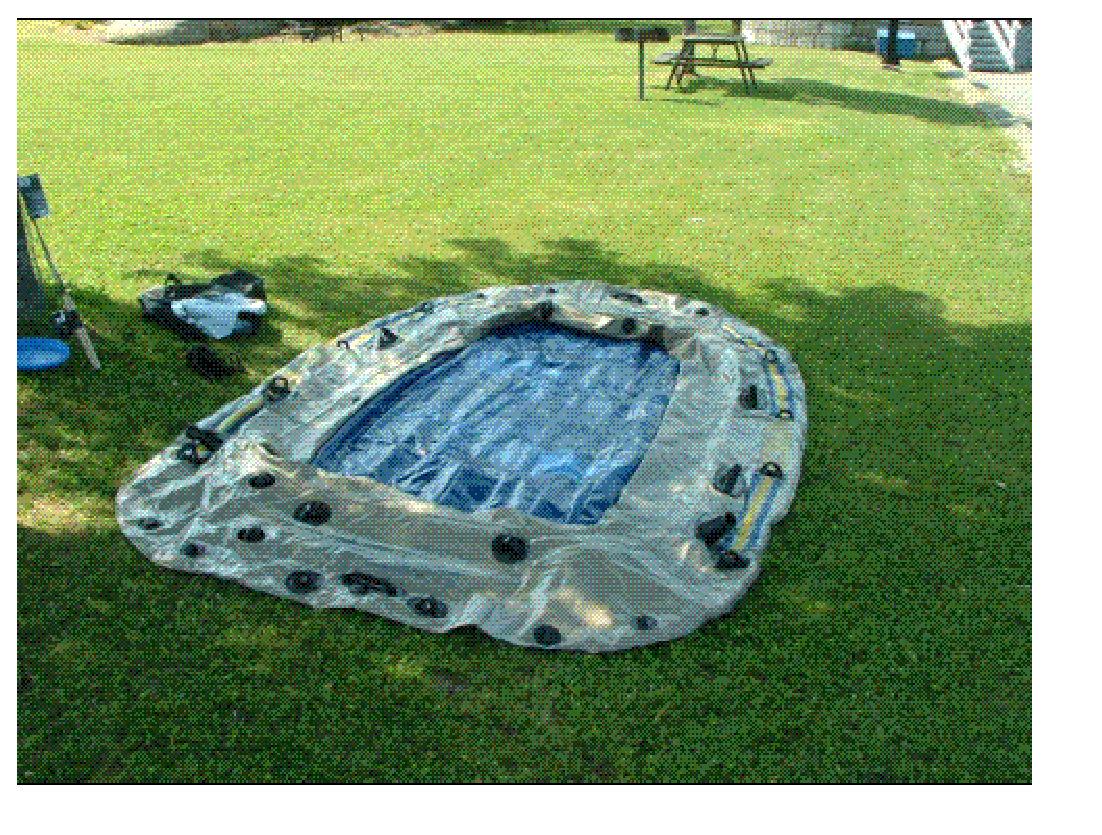
\epsfig{file=fig1.eps,width=3.5in}
Which one of the following is missing in it?
 
 
\noindent{\textbf{\large{
A.}}}
An airplane
 
 
\noindent{\textbf{\large{
B.}}}
A frisbee
 
 
\noindent{\textbf{\large{
C.}}}
Lawn
 
 
\noindent{\textbf{\large{
D.}}}
A table
 
 
\noindent{\textbf{\large{
E.}}}
An air-boat
 
 
\noindent{\textbf{\large{
F.}}}
  Not any of aboves.
 
 
\noindent\vspace{0.05in}{\textbf{\Large{Auto-answer:}}}
 
 
\noindent{\textbf{\large{
A.}}}
An airplane
 
 
\noindent\vspace{0.05in}{\textbf{\Large{End of auto-answer.}}}
 
 
 
\vspace{0.3in}
   
   
\noindent{\textbf{\Large{Total numbers: }}}
   
   
\noindent\begin{tabular}{|l|l|l|l|l|l|l|}
 \hline
Inputs & Calculates & Choices & Layers & Matches & Answer & Solution \\ \hline
           0 & 
           0 & 
           6
  simple  
  & 
           6 & 
           0 & 
  yes & 
  no 
  \\ \hline
 \end{tabular}
   
   
   
   
\noindent\vspace{0.1in}{\textbf{\Large{Calculated values:}}}
   
   
   
   
\noindent\vspace{0.1in}\hspace{-0.08in} {\textbf{\Large{All inputs: }}}
   
   
   
   
\vspace{0.3in}
{\textbf{\LARGE{You have done all the above? A very good beginning, please go ahead.}}}
More constants the
Mass of electron
$m_e$$ =
9.109390 \times 10^{-31} $
kg
,
Universal gas constant
$R$$ =
8.315 $
J/(mol$\cdot $K)
,
$e$$ =
1.60217733 \times 10^{-19} $
C
, and
$m_p$$ =
1.6726231 \times 10^{-27} $
kg
%
may be very helpful.
\vspace{0.3in}
   
   
  
\vspace{0.2in}
  
{\textbf{\Large{QUESTION
33.2 
 (          3,          3,          3)
}}}
  
  
Please choose the correct one from the following statements:
 
 
\noindent{\textbf{\large{
A.}}}
Canada has  %
10 provinces and  %
3 territories.
 
 
\noindent{\textbf{\large{
B.}}}
Canada has  %
34 provinces and  %
39 territories.
 
 
\noindent{\textbf{\large{
C.}}}
Canada has  %
33 provinces and  %
38 territories.
 
 
\noindent{\textbf{\large{
D.}}}
Canada has  %
35 provinces and  %
34 territories.
 
 
\noindent{\textbf{\large{
E.}}}
Canada has  %
37 provinces and  %
37 territories.
 
 
\noindent{\textbf{\large{
F.}}}
 None of above.
 
 
\noindent\vspace{0.05in}{\textbf{\Large{Auto-answer:}}}
 
 
\noindent{\textbf{\large{
A.}}}
Canada has  %
10 provinces and  %
3 territories.
 
 
\noindent\vspace{0.05in}{\textbf{\Large{End of auto-answer.}}}
 
 
   
   
\noindent{\textbf{\Large{Total numbers: }}}
   
   
\noindent\begin{tabular}{|l|l|l|l|l|l|l|}
 \hline
Inputs & Calculates & Choices & Layers & Matches & Answer & Solution \\ \hline
           0 & 
          20 & 
           6
  simple  
  & 
           6 & 
           0 & 
  yes & 
  no 
  \\ \hline
 \end{tabular}
   
   
   
   
\noindent\vspace{0.1in}{\textbf{\Large{Calculated values:}}}
   
   
  
  
\noindent\begin{tabular}{|l|l|l|l|}
\hline
 Sequential & Type & Accuracy & Calculated \\ 
\hline
 
 
  Calculated $           1$ & integer &  & 
  $ 10 $ 
 \\  \hline  
 
 
  Calculated $           2$ & integer &  & 
  $ 3 $ 
 \\  \hline  
 
 
  Calculated $           3$ & integer &  & 
  $ 23 $ 
 \\  \hline  
 
 
  Calculated $           4$ & integer &  & 
  $ 24 $ 
 \\  \hline  
 
 
  Calculated $           5$ & integer &  & 
  $ 25 $ 
 \\  \hline  
 
 
  Calculated $           6$ & integer &  & 
  $ 26 $ 
 \\  \hline  
 
 
  Calculated $           7$ & integer &  & 
  $ 27 $ 
 \\  \hline  
 
 
  Calculated $           8$ & integer &  & 
  $ 28 $ 
 \\  \hline  
 
 
  Calculated $           9$ & integer &  & 
  $ 29 $ 
 \\  \hline  
 
 
  Calculated $          10$ & integer &  & 
  $ 30 $ 
 \\  \hline  
 \end{tabular}
   
   
  
  
\noindent\begin{tabular}{|l|l|l|l|}
\hline
 Sequential & Type & Accuracy & Calculated \\ 
\hline
 
 
  Calculated $          11$ & integer &  & 
  $ 31 $ 
 \\  \hline  
 
 
  Calculated $          12$ & integer &  & 
  $ 32 $ 
 \\  \hline  
 
 
  Calculated $          13$ & integer &  & 
  $ 33 $ 
 \\  \hline  
 
 
  Calculated $          14$ & integer &  & 
  $ 34 $ 
 \\  \hline  
 
 
  Calculated $          15$ & integer &  & 
  $ 35 $ 
 \\  \hline  
 
 
  Calculated $          16$ & integer &  & 
  $ 36 $ 
 \\  \hline  
 
 
  Calculated $          17$ & integer &  & 
  $ 37 $ 
 \\  \hline  
 
 
  Calculated $          18$ & integer &  & 
  $ 38 $ 
 \\  \hline  
 
 
  Calculated $          19$ & integer &  & 
  $ 39 $ 
 \\  \hline  
 
 
  Calculated $          20$ & integer &  & 
  $ 40 $ 
 \\  \hline  
 \end{tabular}
   
   
   
   
\noindent\vspace{0.1in}\hspace{-0.08in} {\textbf{\Large{All inputs: }}}
   
   
  
\vspace{0.2in}
  
{\textbf{\Large{QUESTION
33.3 
 (          5,          5,          5)
}}}
  
  
If any one of the following statements is correct, please fill the box ahead of it with $T$ .
If wrong, fill with $F$.
 
\noindent\begin{tabular}{|l|l|}\hline Your&\hspace{.2in} \\ answer&\hspace{.2in} \\ \hline \end{tabular}
1. $ % 
60$ is an  % 
even number.
 
\noindent\begin{tabular}{|l|l|}\hline Your&\hspace{.2in} \\ answer&\hspace{.2in} \\ \hline \end{tabular}
2.  % 
Kingston is in  % 
Ontario province.
 
\noindent\begin{tabular}{|l|l|}\hline Your&\hspace{.2in} \\ answer&\hspace{.2in} \\ \hline \end{tabular}
3.  % 
$\mathbf{F}=m\mathbf{a}$ is a mathmatical form of
the Newton's Second Law.
 
 
 
\noindent\vspace{0.05in}{\textbf{\Large{Answer:}}}
 
 

 
\noindent\begin{tabular}{|l|l|}\hline The correct & \\
          answer &  % 
$T$ \\ \hline \end{tabular}
1. $ % 
60$ is an  % 
even number.
 
\noindent\begin{tabular}{|l|l|}\hline The correct & \\
          answer &  % 
$T$ \\ \hline \end{tabular}
2.  % 
Kingston is in  % 
Ontario province.
 
\noindent\begin{tabular}{|l|l|}\hline The correct & \\
          answer &  % 
$T$ \\ \hline \end{tabular}
3.  % 
$\mathbf{F}=m\mathbf{a}$ is a mathmatical form of  % 
the Newton's Second Law.
 
 
 
\noindent\vspace{0.05in}{\textbf{\Large{End of Answer.}}}
 
 

 
\vspace{0.3in}
   
   
\noindent{\textbf{\Large{Total numbers: }}}
   
   
\noindent\begin{tabular}{|l|l|l|l|l|l|l|}
 \hline
Inputs & Calculates & Choices & Layers & Matches & Answer & Solution \\ \hline
           6 & 
           3 & 
           0
  & 
           0 & 
           0 & 
  yes & 
  no 
  \\ \hline
 \end{tabular}
   
   
   
   
\noindent\vspace{0.1in}{\textbf{\Large{Calculated values:}}}
   
   
  
  
\noindent\begin{tabular}{|l|l|l|l|}
\hline
 Sequential & Type & Accuracy & Calculated \\ 
\hline
 
 
  Calculated $           1$ & string & $           1 $ ( $          2 $ strings)
 : 
 & $T$
 \\  \hline  
 
 
  Calculated $           2$ & string & $           1 $ ( $          2 $ strings)
 : 
 & $T$
 \\  \hline  
 
 
  Calculated $           3$ & string & $           1 $ ( $          2 $ strings)
 : 
 & $T$
 \\  \hline  
 \end{tabular}
   
   
   
   
\noindent\vspace{0.1in}\hspace{-0.08in} {\textbf{\Large{All inputs: }}}
   
   
  
  
\noindent\begin{tabular}{|l|l|l|l|l|}
\hline
 Sequential & Type & Accuracy & Three inputs & Generated \\ 
\hline
 
 
  INPUT $           1$ & integer &  & $
 1
 , 
 100
 , 
 1
 $ & $ 60 $ 
 \\  \hline  
 
 
  INPUT $           2$ & string & & 
 even & 
  $ <-- $ 
  \\
  & & & 
 odd & 
 \\  \hline  
 
 
  INPUT $           3$ & string & & 
 Toronto & 
  \\
  & & & 
 Kingston & 
  $ <-- $ 
  \\
  & & & 
 Montreal & 
  \\
  & & & 
 Hull & 
 \\  \hline  
 \end{tabular}
   
   
  
  
\noindent\begin{tabular}{|l|l|l|l|l|}
\hline
 Sequential & Type & Accuracy & Three inputs & Generated \\ 
\hline
 
 
  INPUT $           4$ & string & & 
 Ontario & 
  $ <-- $ 
  \\
  & & & 
 Quebec & 
 \\  \hline  
 
 
  INPUT $           5$ & string & & 
 $\mathbf{F}=m\mathbf{a}$ & 
  $ <-- $ 
  \\
  & & & 
 $\left| \mathbf{F}\right| =Gm_1m_2r^{-2}$ & 
 \\  \hline  
 
 
  INPUT $           6$ & string & & 
 the Newton's Second Law & 
  $ <-- $ 
  \\
  & & & 
 Newton's Law of Universal Gravitation & 
 \\  \hline  
 \end{tabular}
   
   
  
\vspace{0.2in}
  
{\textbf{\Large{QUESTION
33.4 
 (          1,          1,          1)
}}}
  
  


\noindent\vspace{0.05in}{\textbf{\Large{Abstract:}}}
This is a simple Newton's Second Law calculation multi-choice problem.  
\noindent\vspace{0.05in}{\textbf{\Large{end of abstract.}}}


 
 
An object is subjected to an external net force $\mathbf{f}=
(20.0 , 9.0 , -4000.0) N$.
Its mass is known as $m= % 
52.0000 kg$. Please choose the
correct accelaration from the following choices.
 
 
 
\noindent{\textbf{\large{
A.}}}
The accelaration is $  %
(
.385,
.17,
-364.54)
ms^{-2} $.
 
 
\noindent{\textbf{\large{
B.}}}
The accelaration is $  %
(
.385,
.60,
-76.923)
ms^{-2} $.
 
 
\noindent{\textbf{\large{
C.}}}
The accelaration is $  %
(
2.64,
.60,
-364.54)
ms^{-2} $.
 
 
\noindent{\textbf{\large{
D.}}}
The accelaration is $  %
(
2.64,
.60,
-76.923)
ms^{-2} $.
 
 
\noindent{\textbf{\large{
E.}}}
The accelaration is $  %
(
2.64,
.17,
-76.923)
ms^{-2} $.
 
 
\noindent{\textbf{\large{
F.}}}
The accelaration is $  %
(
2.64,
.17,
-364.54)
ms^{-2} $.
 
 
\noindent{\textbf{\large{
G.}}}
The accelaration is $  %
(
.385,
.17,
-76.923)
ms^{-2} $.
 
 
\noindent{\textbf{\large{
H.}}}
The accelaration is $  %
(
.385,
.60,
-364.54)
ms^{-2} $.
 
 
\noindent\vspace{0.05in}{\textbf{\Large{Auto-answer:}}}
 
 
\noindent{\textbf{\large{
G.}}}
The accelaration is $  %
(
.385,
.17,
-76.923)
ms^{-2} $.
 
 
\noindent\vspace{0.05in}{\textbf{\Large{End of auto-answer.}}}
 
 
 
 
 
\noindent\vspace{0.05in}{\textbf{\Large{Answer:}}}
 
 

The correct answer from the choices is


\noindent{\textbf{\large{
G.}}}
The accelaration is $  %
(
.385,
.17,
-76.923)
ms^{-2} $.
 
 
 
\noindent\vspace{0.05in}{\textbf{\Large{End of Answer.}}}
 
 

 
 
 
\noindent\vspace{0.1in}{\textbf{\Large{Solution: }}}
 
 

We will use the Newton's Second Law:
 
\[
\mathbf{f}=m\mathbf{a}.
\]
 
Since $\mathbf{f}= % 
(20.0 , 9.0 , -4000.0) N$
and $m= % 
52.0000kg$, bring them into the above equation, then we get
 
\begin{eqnarray*}
\mathbf{a}&=&\frac{\mathbf{f}}m  \\
&=&\frac{ % 
(20.0 , 9.0 , -4000.0) N}{ % 
52.0000kg}  \\
&=& % 
(.385 , .17 , -76.923) ms^{-2}
\end{eqnarray*}
 
 
 
\noindent\vspace{0.1in}{\textbf{\Large{End of Solution.}}}
 
 

 
\vspace{0.3in}
   
   
\noindent{\textbf{\Large{Total numbers: }}}
   
   
\noindent\begin{tabular}{|l|l|l|l|l|l|l|}
 \hline
Inputs & Calculates & Choices & Layers & Matches & Answer & Solution \\ \hline
           2 & 
           1 & 
           8
  & 
           3 & 
           0 & 
  yes & 
  yes 
  \\ \hline
 \end{tabular}
   
   
   
   
\noindent\vspace{0.1in}{\textbf{\Large{Calculated values:}}}
   
   
  
  
\noindent\begin{tabular}{|l|l|l|l|}
\hline
 Sequential & Type & Accuracy & Calculated \\ 
\hline
 
 
  Calculated $           1$ & vector &  
  $           3 $ 
 &  $ .385 $ 
 \\    
  & & 
  $           2 $ 
 &  $ .17 $ 
 \\    
  & & 
  $           5 $ 
 &  $ -76.923 $ 
 \\  \hline  
 \end{tabular}
   
   
   
   
\noindent\vspace{0.1in}\hspace{-0.08in} {\textbf{\Large{All inputs: }}}
   
   
  
  
\noindent\begin{tabular}{|l|l|l|l|l|}
\hline
 Sequential & Type & Accuracy & Three inputs & Generated \\ 
\hline
 
 
  INPUT $           1$ & vector & $          -1 $ & $
20.0
  $ & \\
  & & & $
101.0
  $ & \\
  & & & $
10.0
$ & $ 20.0 $ 
  \\
  & & $          -1 $ & $
2.0
  $ & \\
  & & & $
10.1
  $ & \\
  & & & $
1.0
$ & $ 9.0 $ 
  \\
  & & $          -1 $ & $
-2000.0
  $ & \\
  & & & $
-10001.0
  $ & \\
  & & & $
-1000.0
$ & $ -4000.0 $ 
 \\  \hline  
 
 
  INPUT $           2$ & real & $          -4 $ & $
 50.0000
  $ & \\
  & & &  $
 60.1000
  $ & \\
  & & &  $
 2.0000
 $ & $ 52.0000 $ 
 \\  \hline  
 \end{tabular}
   
   
  
\vspace{0.2in}
  
{\textbf{\Large{QUESTION
33.5 
 (          2,          2,          2)
}}}
  
  
 
An object is subjected to an external net force $\mathbf{f}=(
100.000 ,
2.0000,
-9000.0  )N$. Its mass is known as
$m= % 
50.0000  kg$. Please choose the correct accelaration
from the following choices.
 
 
 
\noindent{\textbf{\large{
A.}}}
The accelaration is
$(
7.8567ms^{-2},
518.40km/h^2,
720.09ms^{-2}
).
$
 
 
\noindent{\textbf{\large{
B.}}}
The accelaration is
$(
7.8567ms^{-2},
518.40km/h^2,
-180.00ms^{-2}
).
$
 
 
\noindent{\textbf{\large{
C.}}}
The accelaration is
$(
2.0000ms^{-2},
518.40km/h^2,
720.09ms^{-2}
).
$
 
 
\noindent{\textbf{\large{
D.}}}
The accelaration is
$(
2.0000ms^{-2},
1545.6km/h^2,
720.09ms^{-2}
).
$
 
 
\noindent{\textbf{\large{
E.}}}
The accelaration is
$(
2.0000ms^{-2},
1545.6km/h^2,
-180.00ms^{-2}
).
$
 
 
\noindent{\textbf{\large{
F.}}}
The accelaration is
$(
7.8567ms^{-2},
1545.6km/h^2,
-180.00ms^{-2}
).
$
 
 
\noindent{\textbf{\large{
G.}}}
 None of these.
 
 
\noindent\vspace{0.05in}{\textbf{\Large{Auto-answer:}}}
 
 
\noindent{\textbf{\large{
G.}}}
 None of these.
 
 
\noindent\vspace{0.05in}{\textbf{\Large{End of auto-answer.}}}
 
 
 
 
 
 
\noindent\vspace{0.1in}{\textbf{\Large{Solution: }}}
 
 

We will use the Newton's Second Law:
 
\[
\mathbf{f}=m\mathbf{a}.
\]
 
Since $\mathbf{f}=( % 
100.000,  % 
2.0000,  % 
-9000.0 )N$
and $m= % 
50.0000kg$, bring them into the above equation, then we get
 
\begin{eqnarray*}
\mathbf{a}&=&\frac{\mathbf{f}}m  \\
&=&\frac{(
100.000 ,
2.0000 ,
-9000.0 )N
}{ % 
50.0000 kg}  \\
&=&(
2.0000 ,
4.0000 \times 10^{-2},
-180.00
)ms^{-2} \\
&=&(
25920. ,
518.40 ,
-2.3328 \times 10^{6}
)km/h^2.
\end{eqnarray*}
 
 
 
\noindent\vspace{0.1in}{\textbf{\Large{End of Solution.}}}
 
 

 
\vspace{0.3in}
   
   
\noindent{\textbf{\Large{Total numbers: }}}
   
   
\noindent\begin{tabular}{|l|l|l|l|l|l|l|}
 \hline
Inputs & Calculates & Choices & Layers & Matches & Answer & Solution \\ \hline
           4 & 
           6 & 
           7
  & 
           3 & 
           0 & 
  yes & 
  yes 
  \\ \hline
 \end{tabular}
   
   
   
   
\noindent\vspace{0.1in}{\textbf{\Large{Calculated values:}}}
   
   
  
  
\noindent\begin{tabular}{|l|l|l|l|}
\hline
 Sequential & Type & Accuracy & Calculated \\ 
\hline
 
 
  Calculated $           1$ & real & $           5 $ & 
 $ 2.0000 $ 
 \\  \hline  
 
 
  Calculated $           2$ & real & $           5 $ & 
 $ 4.0000 \times 10^{-2} $ 
 \\  \hline  
 
 
  Calculated $           3$ & real & $           5 $ & 
 $ -180.00 $ 
 \\  \hline  
 
 
  Calculated $           4$ & real & $           5 $ & 
 $ 25920. $ 
 \\  \hline  
 
 
  Calculated $           5$ & real & $           5 $ & 
 $ 518.40 $ 
 \\  \hline  
 
 
  Calculated $           6$ & real & $           5 $ & 
 $ -2.3328 \times 10^{6} $ 
 \\  \hline  
 \end{tabular}
   
   
   
   
\noindent\vspace{0.1in}\hspace{-0.08in} {\textbf{\Large{All inputs: }}}
   
   
  
  
\noindent\begin{tabular}{|l|l|l|l|l|}
\hline
 Sequential & Type & Accuracy & Three inputs & Generated \\ 
\hline
 
 
  INPUT $           1$ & real & $          -3 $ & $
 20.000
  $ & \\
  & & &  $
 101.000
  $ & \\
  & & &  $
 10.000
 $ & $ 100.000 $ 
 \\  \hline  
 
 
  INPUT $           2$ & real & $          -4 $ & $
 2.0000
  $ & \\
  & & &  $
 10.1000
  $ & \\
  & & &  $
 1.0000
 $ & $ 2.0000 $ 
 \\  \hline  
 
 
  INPUT $           3$ & real & $          -1 $ & $
 -2000.0
  $ & \\
  & & &  $
 -10001.0
  $ & \\
  & & &  $
 -1000.0
 $ & $ -9000.0 $ 
 \\  \hline  
 \end{tabular}
   
   
  
  
\noindent\begin{tabular}{|l|l|l|l|l|}
\hline
 Sequential & Type & Accuracy & Three inputs & Generated \\ 
\hline
 
 
  INPUT $           4$ & real & $          -4 $ & $
 50.0000
  $ & \\
  & & &  $
 60.1000
  $ & \\
  & & &  $
 2.0000
 $ & $ 50.0000 $ 
 \\  \hline  
 \end{tabular}
   
   
  
\vspace{0.2in}
  
{\textbf{\Large{QUESTION
33.6 
 (          4,          4,          4)
}}}
  
  
Considering case-insensitivity, please match the following same strings.
  
  
\begin{tabular}{|l|l|l|}
 \hline
 Column Left & Column Right  & Your choinces \\ 
 \hline
{\textbf{\large{
A.}}}
B
  & 
ER
 & 
 \\ 
 \hline
{\textbf{\large{
B.}}}
asdf(:)
  & 
 a= %
2
 & 
 \\ 
 \hline
{\textbf{\large{
C.}}}
er
  & 
YJH
 & 
 \\ 
 \hline
{\textbf{\large{
D.}}}
yjh
  & 
b
 & 
 \\ 
 \hline
{\textbf{\large{
E.}}}
 A= %
4/ %
2

  & 
ASDF(:)
 & 
 \\ 
 \hline
 \end{tabular}
  
  
 
 
\noindent\vspace{0.05in}{\textbf{\Large{Auto-answer:}}}
  
  
\begin{tabular}{|l|l|l|}
 \hline
 Column Left & Column Right  & Answers       \\ 
 \hline
{\textbf{\large{
A.}}}
B
  & 
ER
 & 
{\textbf{\large{
C.}}}
 \\ 
 \hline
{\textbf{\large{
B.}}}
asdf(:)
  & 
 a= %
2
 & 
{\textbf{\large{
E.}}}
 \\ 
 \hline
{\textbf{\large{
C.}}}
er
  & 
YJH
 & 
{\textbf{\large{
D.}}}
 \\ 
 \hline
{\textbf{\large{
D.}}}
yjh
  & 
b
 & 
{\textbf{\large{
A.}}}
 \\ 
 \hline
{\textbf{\large{
E.}}}
 A= %
4/ %
2

  & 
ASDF(:)
 & 
{\textbf{\large{
B.}}}
 \\ 
 \hline
 \end{tabular}
  
  
 
 
\noindent\vspace{0.05in}{\textbf{\Large{End of auto-answer.}}}
 
 
 
   
   
\noindent{\textbf{\Large{Total numbers: }}}
   
   
\noindent\begin{tabular}{|l|l|l|l|l|l|l|}
 \hline
Inputs & Calculates & Choices & Layers & Matches & Answer & Solution \\ \hline
           2 & 
           1 & 
           0
  & 
          16 & 
           5 & 
  yes & 
  no 
  \\ \hline
 \end{tabular}
   
   
   
   
\noindent\vspace{0.1in}{\textbf{\Large{Calculated values:}}}
   
   
  
  
\noindent\begin{tabular}{|l|l|l|l|}
\hline
 Sequential & Type & Accuracy & Calculated \\ 
\hline
 
 
  Calculated $           1$ & integer &  & 
  $ 2 $ 
 \\  \hline  
 \end{tabular}
   
   
   
   
\noindent\vspace{0.1in}\hspace{-0.08in} {\textbf{\Large{All inputs: }}}
   
   
  
  
\noindent\begin{tabular}{|l|l|l|l|l|}
\hline
 Sequential & Type & Accuracy & Three inputs & Generated \\ 
\hline
 
 
  INPUT $           1$ & integer &  & $
 2
 , 
 8
 , 
 2
 $ & $ 4 $ 
 \\  \hline  
 
 
  INPUT $           2$ & integer &  & $
 2
 , 
 3
 , 
 2
 $ & $ 2 $ 
 \\  \hline  
 \end{tabular}
   
   
   
   
\vspace{0.3in}
{\textbf{\LARGE{You have done all the above? Excellent! Not much left, please continue.}}}
\vspace{0.3in}
   
   
  
\vspace{0.2in}
  
{\textbf{\Large{QUESTION
33.7 
 (          8,         15,         60)
}}}
  
  
 
$ \left( \begin{array}{ccccccccc}
           6 & 
           6 & 
           6 & 
           4 \\ 
           5 & 
           4 & 
           5 & 
           6 \\ 
           4 & 
           4 & 
           5 & 
           4
\end{array}\right) \times
\left( \begin{array}{c}
           2 \\ 
           2 \\ 
           2 \\ 
           2
\end{array}\right) $ =?
 
 
$  % 
 \left( \begin{array}
 {
 c
 c
 }
 \Theta & 
 \eta \\ 
 \rho & 
 \Gamma \\ 
                    \zeta & 
 \Delta \\ 
 \alpha & 
 \Theta
 \end{array} \right)
 \left( \begin{array}
 {
 c
 }
 \beta \\ 
 \beta
 \end{array} \right)
$ =?
 
 
 
\noindent\vspace{0.05in}{\textbf{\Large{Answer:}}}
 
 

 
$\left( \begin{array}{ccccccccccccccc}
           6 & 
           6 & 
           6 & 
           4 \\ 
           5 & 
           4 & 
           5 & 
           6 \\ 
           4 & 
           4 & 
           5 & 
           4
\end{array}\right) \times
\left( \begin{array}{c}
           2 \\ 
           2 \\ 
           2 \\ 
           2
\end{array}\right)  =
\left( \begin{array}{c}
          44 \\ 
          40 \\ 
          34
\end{array}\right)  $
 
$  % 
 \left( \begin{array}
 {
 c
 c
 }
 \Theta & 
 \eta \\ 
 \rho & 
 \Gamma \\ 
                    \zeta & 
 \Delta \\ 
 \alpha & 
 \Theta
 \end{array} \right)
 \left( \begin{array}
 {
 c
 }
 \beta \\ 
 \beta
 \end{array} \right)
=
  \left( \begin{array}
 {
 c
 }
 \Theta \times  \beta   +  \eta \times  \beta \\ 
 \rho \times  \beta   +  \Gamma \times  \beta \\ 
                    \zeta \times  \beta   +  \Delta \times  \beta \\ 
 \alpha \times  \beta   +  \Theta \times  \beta
 \end{array} \right)
$
 
 
 
\noindent\vspace{0.05in}{\textbf{\Large{End of Answer.}}}
 
 

 
 
 
\noindent\vspace{0.1in}{\textbf{\Large{Solution: }}}
 
 

 
 
\noindent\vspace{0.1in}{\textbf{\Large{End of Solution.}}}
 
 

 
\vspace{0.3in}
   
   
\noindent{\textbf{\Large{Total numbers: }}}
   
   
\noindent\begin{tabular}{|l|l|l|l|l|l|l|}
 \hline
Inputs & Calculates & Choices & Layers & Matches & Answer & Solution \\ \hline
           4 & 
           2 & 
           0
  & 
           0 & 
           0 & 
  yes & 
  yes 
  \\ \hline
 \end{tabular}
   
   
   
   
\noindent\vspace{0.1in}{\textbf{\Large{Calculated values:}}}
   
   
  
  
\noindent\begin{tabular}{|l|l|l|l|}
\hline
 Sequential & Type & Accuracy & Calculated \\ 
\hline
 
 
  Calculated $           1$ & i-matrix &  & 
 (size:           3 by           1)
 \\  \hline  
 \end{tabular}
   
   
$\begin{array}{
 c
 }
          44 \\ 
          40 \\ 
          34
 \end{array}  $ 
  
  
\noindent\begin{tabular}{|l|l|l|l|}
\hline
 Sequential & Type & Accuracy & Calculated \\ 
\hline
 
 
  Calculated $           2$ & s-matrix & & 
 (size:           4 by           1)
 \\  \hline  
 \end{tabular}
   
   
 $   \left( \begin{array}
 {
 c
 }
 \Theta \times  \beta   +  \eta \times  \beta \\ 
 \rho \times  \beta   +  \Gamma \times  \beta \\ 
                    \zeta \times  \beta   +  \Delta \times  \beta \\ 
 \alpha \times  \beta   +  \Theta \times  \beta
 \end{array} \right) $ 
   
   
\noindent\vspace{0.1in}\hspace{-0.08in} {\textbf{\Large{All inputs: }}}
   
   
  
  
\noindent\begin{tabular}{|l|l|l|l|l|}
\hline
 Sequential & Type & Accuracy & Three inputs & Generated \\ 
\hline
 
 
  INPUT $           1$ & i-matrix &  & $
 4
 , 
 7
 , 
 1
 $ & (size:           3 by           4)
 \\  \hline  
 \end{tabular}
   
   
 $\begin{array}{
 c
 c
 c
 c
 }
           6 & 
           6 & 
           6 & 
           4 \\ 
           5 & 
           4 & 
           5 & 
           6 \\ 
           4 & 
           4 & 
           5 & 
           4
\end{array}  $ 
  
  
\noindent\begin{tabular}{|l|l|l|l|l|}
\hline
 Sequential & Type & Accuracy & Three inputs & Generated \\ 
\hline
 
 
  INPUT $           2$ & i-matrix &  & $
 2
 , 
 2
 , 
 1
 $ & (size:           4 by           1)
 \\  \hline  
 \end{tabular}
   
   
 $\begin{array}{
 c
 }
           2 \\ 
           2 \\ 
           2 \\ 
           2
\end{array}  $ 
  
  
\noindent\begin{tabular}{|l|l|l|l|l|}
\hline
 Sequential & Type & Accuracy & Three inputs & Generated \\ 
\hline
 
 
  INPUT $           3$ & s-matrix & & 
 $  \alpha $ & 
  \\
  & & & 
 $  \beta $ & 
  \\
  & & & 
 $  \gamma $ & 
  \\
  & & & 
 $  \delta $ & 
  \\
  & & & 
 $  \epsilon $ & 
  \\
  & & & 
 $  \varepsilon $ & 
  \\
  & & & 
 $                     \zeta $ & 
  \\
  & & & 
 $  \eta $ & 
  \\
  & & & 
 $  \rho $ & 
  \\
  & & & 
 $  \sigma $ & 
  \\
  & & & 
 $  \Gamma $ & 
  \\
  & & & 
 $  \Delta $ & 
  \\
  & & & 
 $  \Theta $ & 
  \\
  & & & 
 $  \Lambda $ & 
  \\
  & & & 
 $                     \Xi $ & 
  \\
  & & & 
 $  \Upsilon $ & 
  \\
  & & & 
 $  \Phi $ & 
  \\
  & & & 
 $  \Psi $ & 
  \\
  & & & 
 $  \Omega $ & 
  (size:           4 by           2)
 \\  \hline  
 \end{tabular}
   
   
 $  \left( \begin{array}
 {
 c
 c
 }
 \Theta & 
 \eta \\ 
 \rho & 
 \Gamma \\ 
                    \zeta & 
 \Delta \\ 
 \alpha & 
 \Theta
 \end{array} \right) $ 
  
  
\noindent\begin{tabular}{|l|l|l|l|l|}
\hline
 Sequential & Type & Accuracy & Three inputs & Generated \\ 
\hline
 
 
  INPUT $           4$ & s-matrix & & 
 $  \beta $ & 
  \\
  & & & 
 $  \gamma $ & 
  (size:           2 by           1)
 \\  \hline  
 \end{tabular}
   
   
 $  \left( \begin{array}
 {
 c
 }
 \beta \\ 
 \beta
 \end{array} \right) $ 
  
\vspace{0.2in}
  
{\textbf{\Large{QUESTION
33.8 
 (          7,         14,         50)
}}}
  
  
 
An object is subjected to an external net force $\mathbf{f}=
(20.0 , 4.0 , -3000.0) N$.
Its mass is known as $m= % 
54.0 kg$.
Please choose the correct accelaration from the following choices.
 
 
\noindent{\textbf{\large{
A.}}}
  The accelaration is $  %
(
.370,
.16,
187.26)
ms^{-2} $.
 
 
\noindent{\textbf{\large{
B.}}}
  The accelaration is $  %
(
.370,
7.4 \times 10^{-2},
-55.556)
ms^{-2} $.
 
 
\noindent{\textbf{\large{
C.}}}
  The accelaration is $  %
(
1.82,
.16,
187.26)
ms^{-2} $.
 
 
\noindent{\textbf{\large{
D.}}}
  The accelaration is $  %
(
1.82,
7.4 \times 10^{-2},
187.26)
ms^{-2} $.
 
 
\noindent\vspace{0.05in}{\textbf{\Large{Auto-answer:}}}
 
 
\noindent{\textbf{\large{
B.}}}
  The accelaration is $  %
(
.370,
7.4 \times 10^{-2},
-55.556)
ms^{-2} $.
 
 
\noindent\vspace{0.05in}{\textbf{\Large{End of auto-answer.}}}
 
 
 
 
 
\noindent\vspace{0.1in}{\textbf{\Large{Solution: }}}
 
 

We will use the Newton's Second Law:
 
\[
\mathbf{f}=m\mathbf{a}.
\]
 
Since $\mathbf{f}= % 
(20.0 , 4.0 , -3000.0) N$
and $m= % 
54.0kg$, bring them into the above equation, then we get
 
\begin{eqnarray*}
\mathbf{a}&=&\frac{\mathbf{f}}m  \\
&=&\frac{ % 
(20.0 , 4.0 , -3000.0) N}{ % 
54.0kg}  \\
&=& % 
(.370 , 7.4 \times 10^{-2} , -55.556) ms^{-2}
\end{eqnarray*}
 
 
 
\noindent\vspace{0.1in}{\textbf{\Large{End of Solution.}}}
 
 

 
 
\vspace{0.3in}
   
   
\noindent{\textbf{\Large{Total numbers: }}}
   
   
\noindent\begin{tabular}{|l|l|l|l|l|l|l|}
 \hline
Inputs & Calculates & Choices & Layers & Matches & Answer & Solution \\ \hline
           2 & 
           1 & 
           4
  & 
           3 & 
           0 & 
  yes & 
  yes 
  \\ \hline
 \end{tabular}
   
   
   
   
\noindent\vspace{0.1in}{\textbf{\Large{Calculated values:}}}
   
   
  
  
\noindent\begin{tabular}{|l|l|l|l|}
\hline
 Sequential & Type & Accuracy & Calculated \\ 
\hline
 
 
  Calculated $           1$ & vector &  
  $           3 $ 
 &  $ .370 $ 
 \\    
  & & 
  $           2 $ 
 &  $ 7.4 \times 10^{-2} $ 
 \\    
  & & 
  $           5 $ 
 &  $ -55.556 $ 
 \\  \hline  
 \end{tabular}
   
   
   
   
\noindent\vspace{0.1in}\hspace{-0.08in} {\textbf{\Large{All inputs: }}}
   
   
  
  
\noindent\begin{tabular}{|l|l|l|l|l|}
\hline
 Sequential & Type & Accuracy & Three inputs & Generated \\ 
\hline
 
 
  INPUT $           1$ & vector & $          -1 $ & $
20.0
  $ & \\
  & & & $
101.0
  $ & \\
  & & & $
10.0
$ & $ 20.0 $ 
  \\
  & & $          -1 $ & $
2.0
  $ & \\
  & & & $
10.1
  $ & \\
  & & & $
1.0
$ & $ 4.0 $ 
  \\
  & & $          -1 $ & $
-2000.0
  $ & \\
  & & & $
-10001.0
  $ & \\
  & & & $
-1000.0
$ & $ -3000.0 $ 
 \\  \hline  
 
 
  INPUT $           2$ & real & $          -1 $ & $
 50.0
  $ & \\
  & & &  $
 60.1
  $ & \\
  & & &  $
 2.0
 $ & $ 54.0 $ 
 \\  \hline  
 \end{tabular}
   
   
  
\vspace{0.2in}
  
{\textbf{\Large{QUESTION
33.9 
 (          9,         16,         70)
}}}
  
  


\noindent\vspace{0.05in}{\textbf{\Large{Abstract:}}}
Quadratic Equation constructed from the following first two random (input) integers as roots,  
which of course should not show in the exam papers.  
\noindent\vspace{0.05in}{\textbf{\Large{end of abstract.}}}


 
 
% First root
% Second root

 
Please solve the following equation:
\begin{eqnarray*}
3 \times x^2  % 
+  % 
30
                 \times x    % 
-513 =0
\end{eqnarray*}
 
 
 
\noindent\vspace{0.05in}{\textbf{\Large{Answer:}}}
 
 

9,  % 
-19
 
 
 
\noindent\vspace{0.05in}{\textbf{\Large{End of Answer.}}}
 
 

 
 
 
\noindent\vspace{0.1in}{\textbf{\Large{Solution: }}}
 
 

Roots to the equation
\begin{eqnarray*}
3 \times x^2  % 
+  % 
30
                 \times x    % 
-513 =0
\end{eqnarray*}
are  % 
9 and  % 
-19 .
 
Let us verity  % 
9 first:
$  % 
3 \times x^2  % 
+  % 
30
                 \times x    % 
-513
  = % 
243+( % 
270)+( % 
-513)
  = % 
513+( % 
-513)
  = % 
0
$
 
Then verity  % 
-19:
$  % 
3 \times x^2  % 
+  % 
30
                 \times x    % 
-513
  = % 
1083+( % 
-570)+( % 
-513)
  = % 
513+( % 
-513)
  = % 
0
$
 
 
 
\noindent\vspace{0.1in}{\textbf{\Large{End of Solution.}}}
 
 

 
\vspace{0.3in}
   
   
\noindent{\textbf{\Large{Total numbers: }}}
   
   
\noindent\begin{tabular}{|l|l|l|l|l|l|l|}
 \hline
Inputs & Calculates & Choices & Layers & Matches & Answer & Solution \\ \hline
           3 & 
          13 & 
           0
  & 
           0 & 
           0 & 
  yes & 
  yes 
  \\ \hline
 \end{tabular}
   
   
   
   
\noindent\vspace{0.1in}{\textbf{\Large{Calculated values:}}}
   
   
  
  
\noindent\begin{tabular}{|l|l|l|l|}
\hline
 Sequential & Type & Accuracy & Calculated \\ 
\hline
 
 
  Calculated $           1$ & integer &  & 
  $ 3 $ 
 \\  \hline  
 
 
  Calculated $           2$ & string & $           1 $ ( $          2 $ strings)
 : 
 & +
 \\  \hline  
 
 
  Calculated $           3$ & integer &  & 
  $ 30 $ 
 \\  \hline  
 
 
  Calculated $           4$ & string & $           2 $ ( $          2 $ strings)
 : 
 & 
 \\  \hline  
 
 
  Calculated $           5$ & integer &  & 
  $ -513 $ 
 \\  \hline  
 
 
  Calculated $           6$ & integer &  & 
  $ 243 $ 
 \\  \hline  
 
 
  Calculated $           7$ & integer &  & 
  $ 270 $ 
 \\  \hline  
 
 
  Calculated $           8$ & integer &  & 
  $ 513 $ 
 \\  \hline  
 
 
  Calculated $           9$ & integer &  & 
  $ 0 $ 
 \\  \hline  
 
 
  Calculated $          10$ & integer &  & 
  $ 1083 $ 
 \\  \hline  
 \end{tabular}
   
   
  
  
\noindent\begin{tabular}{|l|l|l|l|}
\hline
 Sequential & Type & Accuracy & Calculated \\ 
\hline
 
 
  Calculated $          11$ & integer &  & 
  $ -570 $ 
 \\  \hline  
 
 
  Calculated $          12$ & integer &  & 
  $ 513 $ 
 \\  \hline  
 
 
  Calculated $          13$ & integer &  & 
  $ 0 $ 
 \\  \hline  
 \end{tabular}
   
   
   
   
\noindent\vspace{0.1in}\hspace{-0.08in} {\textbf{\Large{All inputs: }}}
   
   
  
  
\noindent\begin{tabular}{|l|l|l|l|l|}
\hline
 Sequential & Type & Accuracy & Three inputs & Generated \\ 
\hline
 
 
  INPUT $           1$ & integer &  & $
 -11
 , 
 30
 , 
 4
 $ & $ 9 $ 
 \\  \hline  
 
 
  INPUT $           2$ & integer &  & $
 -31
 , 
 60
 , 
 3
 $ & $ -19 $ 
 \\  \hline  
 
 
  INPUT $           3$ & integer &  & $
 -15
 , 
 15
 , 
 2
 $ & $ 3 $ 
 \\  \hline  
 \end{tabular}
   
   
   
   
   
   
 \vspace{0.2in}
Here are still some constants for use:
 
 
\noindent\begin{tabular}{|l|l|l|}
\hline
Constant & Symbol & Value \\
\hline
 
Mass of proton &
$m_p$ &
 $ 1.6726231 \times 10^{-27} $
kg \\
\hline
 
Boltzmann's constant &
$k$ &
 $ 1.381 \times 10^{-23} $
J/K \\
\hline
 
\end{tabular}
 
Thank you very much for answering these questions!
 
{\textbf{\large{Please be advised}}} that in this paper there are questions from
33.1 through
33.9.
And any one of them may contain more than one sub-question, thus the total number
of sub-questions here is around 14, of which
13 should be answered.
 
   
   
\vspace{2.0in} PAPER TAIL GENERATED.
   
   
   
   
\vspace{1.0in} 
{\textbf{\large{ *** END OF PAPER, THANKS *** }}} 
   
   
\hspace{1.0in} By: 
         239(         26,          34)
   
   
   
   
\newpage 
\setcounter{page}{ 
    34001 } 
   
   
\noindent{\textbf{\huge{THIS IS THE JOURNAL FOR}}}
   
   
 {\textbf{ \Large{ PAPER NUMBER          34 }}}
   
   
\vspace{0.2in}
   
   
\markboth{Journal NOT for examinees !!! {\today}}{Journal NOT for examinees !!! {\today}}
   
   
   
   
   
   
 \vspace{0.2in}
 
 
{\Huge  THIS IS AN EXAMPLE OF}
 
{\Huge  PERSONALIZED TESTS. }
 
If needed, please use the following constants.
 
 
 
\noindent\begin{tabular}{|l|l|l|}
\hline
Constant & Symbol & Value \\
\hline
Acceleration due to earth's gravity &
$g$ &
 $ 9.80 $
m/s$^2$ \\
\hline
Avogadro's number &
$N_A$ &
 $ 6.0221367 \times 10^{23} $
mol$^{-1}$ \\
\hline
Boltzmann's constant &
$k$ &
 $ 1.380658 \times 10^{-23} $
J/K \\
\hline
Coulomb's constant &
$k$ &
 $ 8.99 \times 10^{9} $
N$\cdot $m$^2$/C$^2$ \\
\hline
Electron charge magnitiude &
$e$ &
 $ 1.60217733 \times 10^{-19} $
C \\
\hline
Permeability of free space &
$\mu _0$ &
 $ 1.25663706 \times 10^{-6} $
T$\cdot $m/A \\
\hline
Permittivity of free space &
$\epsilon _0$ &
 $ 8.854187817 \times 10^{-12} $
C$^2$/(N$\cdot $m$^2$) \\
\hline
Pi &
$\pi$ &
 $ 3.14159265 $
$ $ \\
\hline
Planck's constant &
$h$ &
 $ 6.6260755 \times 10^{-34} $
J$\cdot $s \\
\hline
Mass of electron &
$m_e$ &
 $ 9.1093897 \times 10^{-31} $
kg \\
\hline
\end{tabular}
 
 
\noindent\begin{tabular}{|l|l|l|}
\hline
Constant & Symbol & Value \\
\hline
Mass of neutron &
$m_n$ &
 $ 1.6749286 \times 10^{-27} $
kg \\
\hline
Mass of proton &
$m_p$ &
 $ 1.6726231 \times 10^{-27} $
kg \\
\hline
Speed of light in vacuum &
$c$ &
 $ 299792458. $
m/s \\
\hline
Universal gravitational constant &
$G$ &
 $ 6.67259 \times 10^{-11} $
N$\cdot $m$^2$/kg$^2$ \\
\hline
Universal gas constant &
$R$ &
 $ 8.314510 $
J/(mol$\cdot $K) \\
\hline
\end{tabular}
 
 
{\textbf{\large{Please be advised}}} that in this paper there are questions from
34.1 through
34.9.
And any one of them may contain more than one sub-question, thus the total number
of sub-questions here is around 14, of which
13 should be answered.
 
\vspace{0.3in}
 
 
   
   
 PAPER TITLE GENERATED.
   
   
   
\vspace{0.2in}
   
In this paper, big questions will be generated in the following order: 
   
   
            1(          6)
 ,
            2(          2)
 ,
            3(          1)
 ,
            4(          3)
 ,
            5(          5)
 ,
            6(          4)
 ,
            7(          8)
 ,
            8(          7)
 ,
            9(          9)
 .
  
\vspace{0.2in}
  
{\textbf{\Large{QUESTION
34.1 
 (          6)
}}}
  
  
 
{\textbf{\Large{Please answer ONLY
5 of the following
6 questions (Questions
34.1.1 through
34.1.6). }}}
 
Here are still some constants for use in the following questions:
 
 
\noindent\begin{tabular}{|l|l|l|}
\hline
Constant & Symbol & Value \\
\hline
 
Boltzmann's constant &
$k$ &
 $ 1.381 \times 10^{-23} $
J/K \\
\hline
 
Avogadro's number &
$N_A$ &
 $ 6.022 \times 10^{23} $
mol$^{-1}$ \\
\hline
 
Mass of electron &
$m_e$ &
 $ 9.1093897 \times 10^{-31} $
kg \\
\hline
 
\end{tabular}
 
   
\vspace{0.2in}
   
 In this big question of CHOOSE structure,           6 questions will be generat
 ed: 
  
  
            1(          8,         23)
 ,
            2(          9,         24)
 ,
            3(          7,         22)
 ,
            4(         11,         26)
 ,
            5(          6,         21)
 ,
            6(         10,         25)
 .
  
\vspace{0.2in}
  
{\textbf{\Large{Question
34.1.1 
 (          6,          8,         23)
}}}
  
  
 
An object is subjected to an external net force $\mathbf{f}=(
70.0 ,
2.0,
-2000.0  )N$. Its mass is known as
$m= % 
52.0  kg$. Please choose the correct accelaration
from the following choices.
 
 
 
\noindent{\textbf{\large{
A.}}}
The accelaration is
$(
6.5126ms^{-2},
3.8462 \times 10^{-2}ms^{-2},
-498462.km/h^2
).
$
 
 
\noindent{\textbf{\large{
B.}}}
The accelaration is
$(
6.5126ms^{-2},
.10556ms^{-2},
1.7228 \times 10^{6}km/h^2
).
$
 
 
\noindent{\textbf{\large{
C.}}}
The accelaration is
$(
1.3462ms^{-2},
3.8462 \times 10^{-2}ms^{-2},
-498462.km/h^2
).
$
 
 
\noindent{\textbf{\large{
D.}}}
The accelaration is
$(
6.5126ms^{-2},
3.8462 \times 10^{-2}ms^{-2},
1.7228 \times 10^{6}km/h^2
).
$
 
 
\noindent{\textbf{\large{
E.}}}
none of these.
 
 
\noindent\vspace{0.05in}{\textbf{\Large{Auto-answer:}}}
 
 
\noindent{\textbf{\large{
C.}}}
The accelaration is
$(
1.3462ms^{-2},
3.8462 \times 10^{-2}ms^{-2},
-498462.km/h^2
).
$
 
 
\noindent\vspace{0.05in}{\textbf{\Large{End of auto-answer.}}}
 
 
 
 
 
 
\noindent\vspace{0.1in}{\textbf{\Large{Solution: }}}
 
 

We will use the Newton's Second Law:
 
\[
\mathbf{f}=m\mathbf{a}.
\]
 
Since $\mathbf{f}=( % 
70.0,  % 
2.0,  % 
-2000.0 )N$
and $m= % 
52.0kg$, bring them into the above equation, then we get
 
\begin{eqnarray*}
\mathbf{a}&=&\frac{\mathbf{f}}m  \\
&=&\frac{(
70.0 ,
2.0 ,
-2000.0 )N
}{ % 
52.0 kg}  \\
&=&(
1.3462 ,
3.8462 \times 10^{-2},
-38.462
)ms^{-2} \\
&=&(
17446. ,
498.46 ,
-498462.
)km/h^2.
\end{eqnarray*}
 
 
 
\noindent\vspace{0.1in}{\textbf{\Large{End of Solution.}}}
 
 

 
\vspace{0.3in}
   
   
\noindent{\textbf{\Large{Total numbers: }}}
   
   
\noindent\begin{tabular}{|l|l|l|l|l|l|l|}
 \hline
Inputs & Calculates & Choices & Layers & Matches & Answer & Solution \\ \hline
           4 & 
           6 & 
           5
  & 
           3 & 
           0 & 
  yes & 
  yes 
  \\ \hline
 \end{tabular}
   
   
   
   
\noindent\vspace{0.1in}{\textbf{\Large{Calculated values:}}}
   
   
  
  
\noindent\begin{tabular}{|l|l|l|l|}
\hline
 Sequential & Type & Accuracy & Calculated \\ 
\hline
 
 
  Calculated $           1$ & real & $           5 $ & 
 $ 1.3462 $ 
 \\  \hline  
 
 
  Calculated $           2$ & real & $           5 $ & 
 $ 3.8462 \times 10^{-2} $ 
 \\  \hline  
 
 
  Calculated $           3$ & real & $           5 $ & 
 $ -38.462 $ 
 \\  \hline  
 
 
  Calculated $           4$ & real & $           5 $ & 
 $ 17446. $ 
 \\  \hline  
 
 
  Calculated $           5$ & real & $           5 $ & 
 $ 498.46 $ 
 \\  \hline  
 
 
  Calculated $           6$ & real & $           5 $ & 
 $ -498462. $ 
 \\  \hline  
 \end{tabular}
   
   
   
   
\noindent\vspace{0.1in}\hspace{-0.08in} {\textbf{\Large{All inputs: }}}
   
   
  
  
\noindent\begin{tabular}{|l|l|l|l|l|}
\hline
 Sequential & Type & Accuracy & Three inputs & Generated \\ 
\hline
 
 
  INPUT $           1$ & real & $          -1 $ & $
 20.0
  $ & \\
  & & &  $
 101.0
  $ & \\
  & & &  $
 10.0
 $ & $ 70.0 $ 
 \\  \hline  
 
 
  INPUT $           2$ & real & $          -1 $ & $
 2.0
  $ & \\
  & & &  $
 10.1
  $ & \\
  & & &  $
 1.0
 $ & $ 2.0 $ 
 \\  \hline  
 
 
  INPUT $           3$ & real & $          -1 $ & $
 -2000.0
  $ & \\
  & & &  $
 -10001.0
  $ & \\
  & & &  $
 -1000.0
 $ & $ -2000.0 $ 
 \\  \hline  
 \end{tabular}
   
   
  
  
\noindent\begin{tabular}{|l|l|l|l|l|}
\hline
 Sequential & Type & Accuracy & Three inputs & Generated \\ 
\hline
 
 
  INPUT $           4$ & real & $          -1 $ & $
 50.0
  $ & \\
  & & &  $
 60.1
  $ & \\
  & & &  $
 2.0
 $ & $ 52.0 $ 
 \\  \hline  
 \end{tabular}
   
   
  
\vspace{0.2in}
  
{\textbf{\Large{Question
34.1.2 
 (          6,          9,         24)
}}}
  
  
Let us use Newton's Law of Universal Gravitation to calculate the force
of the Sun acting on the eight planets. Let us suppose the mass of the
Sun is $ % 
6.00 \times 10^{24} kg$. With the mass and the
distance to the Sun of each planet in the following table, please fill
the blanks for the forces.
 
\vspace{0.2in}
 
 
\begin{tabular}{|l|l|l|l|}
\hline
The Planet & Mass ($kg$) & Distanace from Sun ($m$) & The Force ($N$)\\
\hline
Mercury  &
           $ % 
7.00000000 \times 10^{24} $   &
             $ % 
8.000000000 \times 10^{24} $    &
\\  \hline
Venus    &
           $ % 
4.00 \times 10^{24} $    &
             $ % 
6.00 \times 10^{24} $    &
\\  \hline
Earth    &
           $ % 
5.00 \times 10^{24} $    &
             $ % 
7.00 \times 10^{24} $    &
\\   \hline
Mars     &
           $ % 
6.00 \times 10^{24} $    &
             $ % 
7.00 \times 10^{24} $    &
\\   \hline
Jupiter  &
           $ % 
4.00 \times 10^{24} $    &
             $ % 
4.00 \times 10^{24} $    &
\\  \hline
Saturn   &
           $ % 
4.00 \times 10^{24}$    &
             $ % 
7.00 \times 10^{24}$    &
\\  \hline
Uranus   &
           $ % 
3.00 \times 10^{24} $    &
             $ % 
3.00 \times 10^{24} $    &
\\  \hline
Neptune  &
           $ % 
7.00 \times 10^{24} $    &
             $ % 
3.00 \times 10^{24} $    &
\\  \hline
 
\end{tabular}
 
 
 
 
\noindent\vspace{0.1in}{\textbf{\Large{Solution: }}}
 
 

By using Newton's Law of Universal Gravitation:
\[
F=G \frac{(Sun's \hspace{0.1in} mass) \times (Planet's \hspace{0.1in} mass)} { (distance)^2},
\]
where
$ G= % 
6.67 \times 10^{-11}N m^{2}(kg)^{-2}$ , the forces can be easily calculated as
 
\vspace{0.2in}
 
 
\begin{tabular}{|l|l|l|l|}
\hline
The Planet & Mass ($kg$) & Distanace from Sun ($m$) & The Force ($N$)\\
\hline
Mercury  &
           $ % 
7.00000000 \times 10^{24} $   &
             $ % 
8.000000000 \times 10^{24} $    & $ % 
4.38 \times 10^{-11} $
\\  \hline
Venus    &
           $  % 
4.00 \times 10^{24}  $     &
             $ % 
6.00 \times 10^{24} $    & $ % 
4.45 \times 10^{-11} $
\\  \hline
Earth    &
           $  % 
5.00 \times 10^{24}  $     &
             $ % 
7.00 \times 10^{24} $    & $ % 
4.08 \times 10^{-11} $
\\   \hline
Mars     &
           $  % 
6.00 \times 10^{24} $     &
             $ % 
7.00 \times 10^{24} $    & $ % 
4.90 \times 10^{-11} $
\\   \hline
Jupiter  &
           $  % 
4.00 \times 10^{24} $    &
             $ % 
4.00 \times 10^{24} $    & $ % 
1.00 \times 10^{-10} $
\\  \hline
Saturn   &
           $  % 
4.00 \times 10^{24} $    &
             $ % 
7.00 \times 10^{24}  $    & $ % 
3.27 \times 10^{-11} $
\\  \hline
Uranus   &
           $  % 
3.00 \times 10^{24} $    &
             $ % 
3.00 \times 10^{24} $    & $ % 
1.33 \times 10^{-10} $
\\  \hline
Neptune  &
           $  % 
7.00 \times 10^{24} $    &
             $ % 
3.00 \times 10^{24} $    & $ % 
3.11 \times 10^{-10} $
\\  \hline
 
\end{tabular}
 
 
 
 
\noindent\vspace{0.1in}{\textbf{\Large{End of Solution.}}}
 
 

 
 
 
 
\noindent\vspace{0.05in}{\textbf{\Large{Answer:}}}
 
 

By using Newton's Law of Universal Gravitation:
\[
F=G \frac{(Sun's \hspace{0.1in} mass) \times (Planet's \hspace{0.1in} mass)} { (distance)^2},
\]
where
$ G= % 
6.67 \times 10^{-11} N m^{2}(kg)^{-2}$ , the forces can be easily calculated as
 
\vspace{0.2in}
 
 
\begin{tabular}{|l|l|l|l|}
\hline
The Planet & Mass ($kg$) & Distanace from Sun ($m$) & The Force ($N$)\\
\hline
Mercury  &
           $ % 
7.00000000 \times 10^{24}  $   &
             $ % 
8.000000000 \times 10^{24}$    & $ % 
4.38 \times 10^{-11} $
\\  \hline
Venus    &
           $  % 
4.00 \times 10^{24}  $     &
             $ % 
6.00 \times 10^{24} $    & $ % 
4.45 \times 10^{-11} $
\\  \hline
Earth    &
           $  % 
5.00 \times 10^{24}$     &
             $ % 
7.00 \times 10^{24} $    & $ % 
4.08 \times 10^{-11} $
\\   \hline
Mars     &
           $  % 
6.00 \times 10^{24} $     &
             $ % 
7.00 \times 10^{24}$    & $ % 
4.90 \times 10^{-11} $
\\   \hline
Jupiter  &
           $  % 
4.00 \times 10^{24}  $    &
             $ % 
4.00 \times 10^{24} $    & $ % 
1.00 \times 10^{-10}3 $
\\  \hline
Saturn   &
           $  % 
4.00 \times 10^{24}   $    &
             $ % 
7.00 \times 10^{24}  $    & $ % 
3.27 \times 10^{-11} $
\\  \hline
Uranus   &
           $  % 
3.00 \times 10^{24} $    &
             $ % 
3.00 \times 10^{24}$    & $ % 
1.33 \times 10^{-10} $
\\  \hline
Neptune  &
           $  % 
7.00 \times 10^{24}  $    &
             $ % 
3.00 \times 10^{24} $    & $ % 
3.11 \times 10^{-10} $
\\  \hline
 
\end{tabular}
 
 
 
 
\noindent\vspace{0.05in}{\textbf{\Large{End of Answer.}}}
 
 

 
\vspace{0.3in}
   
   
\noindent{\textbf{\Large{Total numbers: }}}
   
   
\noindent\begin{tabular}{|l|l|l|l|l|l|l|}
 \hline
Inputs & Calculates & Choices & Layers & Matches & Answer & Solution \\ \hline
          19 & 
           8 & 
           0
  & 
           0 & 
           0 & 
  yes & 
  yes 
  \\ \hline
 \end{tabular}
   
   
   
   
\noindent\vspace{0.1in}{\textbf{\Large{Calculated values:}}}
   
   
  
  
\noindent\begin{tabular}{|l|l|l|l|}
\hline
 Sequential & Type & Accuracy & Calculated \\ 
\hline
 
 
  Calculated $           1$ & real & $           3 $ & 
 $ 4.38 \times 10^{-11} $ 
 \\  \hline  
 
 
  Calculated $           2$ & real & $           3 $ & 
 $ 4.45 \times 10^{-11} $ 
 \\  \hline  
 
 
  Calculated $           3$ & real & $           3 $ & 
 $ 4.08 \times 10^{-11} $ 
 \\  \hline  
 
 
  Calculated $           4$ & real & $           3 $ & 
 $ 4.90 \times 10^{-11} $ 
 \\  \hline  
 
 
  Calculated $           5$ & real & $           3 $ & 
 $ 1.00 \times 10^{-10} $ 
 \\  \hline  
 
 
  Calculated $           6$ & real & $           3 $ & 
 $ 3.27 \times 10^{-11} $ 
 \\  \hline  
 
 
  Calculated $           7$ & real & $           3 $ & 
 $ 1.33 \times 10^{-10} $ 
 \\  \hline  
 
 
  Calculated $           8$ & real & $           3 $ & 
 $ 3.11 \times 10^{-10} $ 
 \\  \hline  
 \end{tabular}
   
   
   
   
\noindent\vspace{0.1in}\hspace{-0.08in} {\textbf{\Large{All inputs: }}}
   
   
  
  
\noindent\begin{tabular}{|l|l|l|l|l|}
\hline
 Sequential & Type & Accuracy & Three inputs & Generated \\ 
\hline
 
 
  INPUT $           1$ & real & $          22 $ & $
 2.00 \times 10^{24}
  $ & \\
  & & &  $
 1.010 \times 10^{25}
  $ & \\
  & & &  $
 10.0 \times 10^{23}
 $ & $ 6.00 \times 10^{24} $ 
 \\  \hline  
 
 
  INPUT $           2$ & real & $          16 $ & $
 2.00000000 \times 10^{24}
  $ & \\
  & & &  $
 1.010000000 \times 10^{25}
  $ & \\
  & & &  $
 10.0000000 \times 10^{23}
 $ & $ 7.00000000 \times 10^{24} $ 
 \\  \hline  
 
 
  INPUT $           3$ & real & $          15 $ & $
 2.000000000 \times 10^{24}
  $ & \\
  & & &  $
 1.0100000000 \times 10^{25}
  $ & \\
  & & &  $
 10.00000000 \times 10^{23}
 $ & $ 8.000000000 \times 10^{24} $ 
 \\  \hline  
 \end{tabular}
   
   
  
  
\noindent\begin{tabular}{|l|l|l|l|l|}
\hline
 Sequential & Type & Accuracy & Three inputs & Generated \\ 
\hline
 
 
  INPUT $           4$ & real & $          22 $ & $
 2.00 \times 10^{24}
  $ & \\
  & & &  $
 1.010 \times 10^{25}
  $ & \\
  & & &  $
 10.0 \times 10^{23}
 $ & $ 4.00 \times 10^{24} $ 
 \\  \hline  
 
 
  INPUT $           5$ & real & $          22 $ & $
 2.00 \times 10^{24}
  $ & \\
  & & &  $
 1.010 \times 10^{25}
  $ & \\
  & & &  $
 10.0 \times 10^{23}
 $ & $ 6.00 \times 10^{24} $ 
 \\  \hline  
 
 
  INPUT $           6$ & real & $          22 $ & $
 2.00 \times 10^{24}
  $ & \\
  & & &  $
 1.010 \times 10^{25}
  $ & \\
  & & &  $
 10.0 \times 10^{23}
 $ & $ 5.00 \times 10^{24} $ 
 \\  \hline  
 \end{tabular}
   
   
  
  
\noindent\begin{tabular}{|l|l|l|l|l|}
\hline
 Sequential & Type & Accuracy & Three inputs & Generated \\ 
\hline
 
 
  INPUT $           7$ & real & $          22 $ & $
 2.00 \times 10^{24}
  $ & \\
  & & &  $
 1.010 \times 10^{25}
  $ & \\
  & & &  $
 10.0 \times 10^{23}
 $ & $ 7.00 \times 10^{24} $ 
 \\  \hline  
 
 
  INPUT $           8$ & real & $          22 $ & $
 2.00 \times 10^{24}
  $ & \\
  & & &  $
 1.010 \times 10^{25}
  $ & \\
  & & &  $
 10.0 \times 10^{23}
 $ & $ 6.00 \times 10^{24} $ 
 \\  \hline  
 
 
  INPUT $           9$ & real & $          22 $ & $
 2.00 \times 10^{24}
  $ & \\
  & & &  $
 1.010 \times 10^{25}
  $ & \\
  & & &  $
 10.0 \times 10^{23}
 $ & $ 7.00 \times 10^{24} $ 
 \\  \hline  
 \end{tabular}
   
   
  
  
\noindent\begin{tabular}{|l|l|l|l|l|}
\hline
 Sequential & Type & Accuracy & Three inputs & Generated \\ 
\hline
 
 
  INPUT $          10$ & real & $          22 $ & $
 2.00 \times 10^{24}
  $ & \\
  & & &  $
 1.010 \times 10^{25}
  $ & \\
  & & &  $
 10.0 \times 10^{23}
 $ & $ 4.00 \times 10^{24} $ 
 \\  \hline  
 
 
  INPUT $          11$ & real & $          22 $ & $
 2.00 \times 10^{24}
  $ & \\
  & & &  $
 1.010 \times 10^{25}
  $ & \\
  & & &  $
 10.0 \times 10^{23}
 $ & $ 4.00 \times 10^{24} $ 
 \\  \hline  
 
 
  INPUT $          12$ & real & $          22 $ & $
 2.00 \times 10^{24}
  $ & \\
  & & &  $
 1.010 \times 10^{25}
  $ & \\
  & & &  $
 10.0 \times 10^{23}
 $ & $ 4.00 \times 10^{24} $ 
 \\  \hline  
 \end{tabular}
   
   
  
  
\noindent\begin{tabular}{|l|l|l|l|l|}
\hline
 Sequential & Type & Accuracy & Three inputs & Generated \\ 
\hline
 
 
  INPUT $          13$ & real & $          22 $ & $
 2.00 \times 10^{24}
  $ & \\
  & & &  $
 1.010 \times 10^{25}
  $ & \\
  & & &  $
 10.0 \times 10^{23}
 $ & $ 7.00 \times 10^{24} $ 
 \\  \hline  
 
 
  INPUT $          14$ & real & $          22 $ & $
 2.00 \times 10^{24}
  $ & \\
  & & &  $
 1.010 \times 10^{25}
  $ & \\
  & & &  $
 10.0 \times 10^{23}
 $ & $ 3.00 \times 10^{24} $ 
 \\  \hline  
 
 
  INPUT $          15$ & real & $          22 $ & $
 2.00 \times 10^{24}
  $ & \\
  & & &  $
 1.010 \times 10^{25}
  $ & \\
  & & &  $
 10.0 \times 10^{23}
 $ & $ 3.00 \times 10^{24} $ 
 \\  \hline  
 \end{tabular}
   
   
  
  
\noindent\begin{tabular}{|l|l|l|l|l|}
\hline
 Sequential & Type & Accuracy & Three inputs & Generated \\ 
\hline
 
 
  INPUT $          16$ & real & $          22 $ & $
 2.00 \times 10^{24}
  $ & \\
  & & &  $
 1.010 \times 10^{25}
  $ & \\
  & & &  $
 10.0 \times 10^{23}
 $ & $ 7.00 \times 10^{24} $ 
 \\  \hline  
 
 
  INPUT $          17$ & real & $          22 $ & $
 2.00 \times 10^{24}
  $ & \\
  & & &  $
 1.010 \times 10^{25}
  $ & \\
  & & &  $
 10.0 \times 10^{23}
 $ & $ 3.00 \times 10^{24} $ 
 \\  \hline  
 
 
  INPUT $          18$ & real & $         -13 $ & $
 6.67 \times 10^{-11}
  $ & \\
  & & &  $
 6.67 \times 10^{-11}
  $ & \\
  & & &  $
 1.00 \times 10^{-11}
 $ & $ 6.67 \times 10^{-11} $ 
 \\  \hline  
 \end{tabular}
   
   
  
  
\noindent\begin{tabular}{|l|l|l|l|l|}
\hline
 Sequential & Type & Accuracy & Three inputs & Generated \\ 
\hline
 
 
  INPUT $          19$ & real & $         -13 $ & $
 6.67 \times 10^{-11}
  $ & \\
  & & &  $
 6.67 \times 10^{-11}
  $ & \\
  & & &  $
 1.00 \times 10^{-11}
 $ & $ 6.67 \times 10^{-11} $ 
 \\  \hline  
 \end{tabular}
   
   
  
\vspace{0.2in}
  
{\textbf{\Large{Question
34.1.3 
 (          6,          7,         22)
}}}
  
  
 
An object is subjected to an external net force $\mathbf{f}=(
30.0 ,
8.0,
-8000.0  )N$. Its mass is known as
$m= % 
54.0  kg$. Please choose the correct accelaration
from the following choices.
 
 
 
\noindent{\textbf{\large{
A.}}}
The accelaration (vector) is
$(
7200.0,
1920.0 ,
-1.9200 \times 10^{6}
)km/h^2.
$
 
 
\noindent{\textbf{\large{
B.}}}
The accelaration (vector) is
$(
19056.,
1920.0 ,
-8.8002 \times 10^{6}
)km/h^2.
$
 
 
\noindent{\textbf{\large{
C.}}}
The accelaration (vector) is
$(
35393.,
1920.0 ,
-7.4286 \times 10^{6}
)km/h^2.
$
 
 
\noindent{\textbf{\large{
D.}}}
The accelaration (vector) is
$(
33646.,
1920.0 ,
-7.4286 \times 10^{6}
)km/h^2.
$
 
 
\noindent{\textbf{\large{
E.}}}
The accelaration (vector) is
$(
19056.,
1920.0 ,
-7.4286 \times 10^{6}
)km/h^2.
$
 
 
\noindent{\textbf{\large{
F.}}}
The accelaration (vector) is
$(
33646.,
1920.0 ,
6.5973 \times 10^{6}
)km/h^2.
$
 
 
\noindent{\textbf{\large{
G.}}}
The accelaration (vector) is
$(
7200.0,
1920.0 ,
-8.8002 \times 10^{6}
)km/h^2.
$
 
 
\noindent{\textbf{\large{
H.}}}
The accelaration (vector) is
$(
19056.,
1920.0 ,
6.5973 \times 10^{6}
)km/h^2.
$
 
 
\noindent{\textbf{\large{
I.}}}
The accelaration (vector) is
$(
33646.,
1920.0 ,
-1.9200 \times 10^{6}
)km/h^2.
$
 
 
\noindent{\textbf{\large{
J.}}}
The accelaration (vector) is
$(
33646.,
1920.0 ,
-8.8002 \times 10^{6}
)km/h^2.
$
 
 
\noindent{\textbf{\large{
K.}}}
The accelaration (vector) is
$(
7200.0,
1920.0 ,
-7.4286 \times 10^{6}
)km/h^2.
$
 
 
\noindent{\textbf{\large{
L.}}}
The accelaration (vector) is
$(
19056.,
1920.0 ,
-1.9200 \times 10^{6}
)km/h^2.
$
 
 
\noindent\vspace{0.05in}{\textbf{\Large{Auto-answer:}}}
 
 
\noindent{\textbf{\large{
A.}}}
The accelaration (vector) is
$(
7200.0,
1920.0 ,
-1.9200 \times 10^{6}
)km/h^2.
$
 
 
\noindent\vspace{0.05in}{\textbf{\Large{End of auto-answer.}}}
 
 
 
 
 
 
\noindent\vspace{0.1in}{\textbf{\Large{Solution: }}}
 
 

We will use the Newton's Second Law:
 
\[
\mathbf{f}=m\mathbf{a}.
\]
 
Since $\mathbf{f}=( % 
30.0,  % 
8.0,  % 
-8000.0 )N$
and $m= % 
54.0 kg$, bring them into the above equation, then we get
 
\begin{eqnarray*}
\mathbf{a}&=&\frac{\mathbf{f}}m  \\
&=&\frac{(
30.0 ,
8.0 ,
-8000.0 )N
}{ % 
54.0 kg}  \\
&=&(
.55556 ,
.14815,
-148.15
)ms^{-2} \\
&=&(
7200.0 ,
1920.0 ,
-1.9200 \times 10^{6}
)km/h^2.
\end{eqnarray*}
 
 
 
\noindent\vspace{0.1in}{\textbf{\Large{End of Solution.}}}
 
 

 
 
\vspace{0.3in}
   
   
\noindent{\textbf{\Large{Total numbers: }}}
   
   
\noindent\begin{tabular}{|l|l|l|l|l|l|l|}
 \hline
Inputs & Calculates & Choices & Layers & Matches & Answer & Solution \\ \hline
           4 & 
           6 & 
          12
  & 
           2 & 
           0 & 
  yes & 
  yes 
  \\ \hline
 \end{tabular}
   
   
   
   
\noindent\vspace{0.1in}{\textbf{\Large{Calculated values:}}}
   
   
  
  
\noindent\begin{tabular}{|l|l|l|l|}
\hline
 Sequential & Type & Accuracy & Calculated \\ 
\hline
 
 
  Calculated $           1$ & real & $           5 $ & 
 $ .55556 $ 
 \\  \hline  
 
 
  Calculated $           2$ & real & $           5 $ & 
 $ .14815 $ 
 \\  \hline  
 
 
  Calculated $           3$ & real & $           5 $ & 
 $ -148.15 $ 
 \\  \hline  
 
 
  Calculated $           4$ & real & $           5 $ & 
 $ 7200.0 $ 
 \\  \hline  
 
 
  Calculated $           5$ & real & $           5 $ & 
 $ 1920.0 $ 
 \\  \hline  
 
 
  Calculated $           6$ & real & $           5 $ & 
 $ -1.9200 \times 10^{6} $ 
 \\  \hline  
 \end{tabular}
   
   
   
   
\noindent\vspace{0.1in}\hspace{-0.08in} {\textbf{\Large{All inputs: }}}
   
   
  
  
\noindent\begin{tabular}{|l|l|l|l|l|}
\hline
 Sequential & Type & Accuracy & Three inputs & Generated \\ 
\hline
 
 
  INPUT $           1$ & real & $          -1 $ & $
 20.0
  $ & \\
  & & &  $
 101.0
  $ & \\
  & & &  $
 10.0
 $ & $ 30.0 $ 
 \\  \hline  
 
 
  INPUT $           2$ & real & $          -1 $ & $
 2.0
  $ & \\
  & & &  $
 10.1
  $ & \\
  & & &  $
 1.0
 $ & $ 8.0 $ 
 \\  \hline  
 
 
  INPUT $           3$ & real & $          -1 $ & $
 -2000.0
  $ & \\
  & & &  $
 -10001.0
  $ & \\
  & & &  $
 -1000.0
 $ & $ -8000.0 $ 
 \\  \hline  
 \end{tabular}
   
   
  
  
\noindent\begin{tabular}{|l|l|l|l|l|}
\hline
 Sequential & Type & Accuracy & Three inputs & Generated \\ 
\hline
 
 
  INPUT $           4$ & real & $          -1 $ & $
 50.0
  $ & \\
  & & &  $
 60.1
  $ & \\
  & & &  $
 2.0
 $ & $ 54.0 $ 
 \\  \hline  
 \end{tabular}
   
   
  
\vspace{0.2in}
  
{\textbf{\Large{Question
34.1.4 
 (          6,         11,         26)
}}}
  
  
In a hotel, the possiblity of  % 
smoking customer is
$a =  % 
.130$, and the possiblity of  % 
 under 30 years old customer is $ b =  % 
.9200$.
Please calculate the possiblity of  % 
 non-smoking and  % 
equal or above 30 years old customer.
 
 
 
\noindent\vspace{0.1in}{\textbf{\Large{Solution: }}}
 
 

Since the possiblity of  % 
smoking customer is $ a =  % 
.130 $,
and the possiblity of  % 
 under 30 years old customer is $ b =  % 
.9200 $,
the possiblity of  % 
non-smoking customer is $ c = 1.0 - a = 1.0 -
.130
=  % 
.870 $ and the possiblity of  % 
equal or above 30 years old
customer is $ d = 1.0 - b = 1.0 -  % 
.9200 =  % 
8.000 \times 10^{-2}  $.
So the possibility of  % 
 non-smoking and  % 
equal or above 30 years old
customer is $ c \times d =  % 
6.96 \times 10^{-2} $.
 
 
 
\noindent\vspace{0.1in}{\textbf{\Large{End of Solution.}}}
 
 

 
 
 
\noindent\vspace{0.05in}{\textbf{\Large{Answer:}}}
 
 

The possibility of  % 
 non-smoking and  % 
equal or above 30 years old
customer is $ (1-a)(1-b) =  % 
6.96 \times 10^{-2} $.
 
 
\noindent\vspace{0.05in}{\textbf{\Large{End of Answer.}}}
 
 

 
\vspace{0.3in}
   
   
\noindent{\textbf{\Large{Total numbers: }}}
   
   
\noindent\begin{tabular}{|l|l|l|l|l|l|l|}
 \hline
Inputs & Calculates & Choices & Layers & Matches & Answer & Solution \\ \hline
           4 & 
           3 & 
           0
  & 
           0 & 
           0 & 
  yes & 
  yes 
  \\ \hline
 \end{tabular}
   
   
   
   
\noindent\vspace{0.1in}{\textbf{\Large{Calculated values:}}}
   
   
  
  
\noindent\begin{tabular}{|l|l|l|l|}
\hline
 Sequential & Type & Accuracy & Calculated \\ 
\hline
 
 
  Calculated $           1$ & real & $           3 $ & 
 $ .870 $ 
 \\  \hline  
 
 
  Calculated $           2$ & real & $           4 $ & 
 $ 8.000 \times 10^{-2} $ 
 \\  \hline  
 
 
  Calculated $           3$ & real & $           3 $ & 
 $ 6.96 \times 10^{-2} $ 
 \\  \hline  
 \end{tabular}
   
   
   
   
\noindent\vspace{0.1in}\hspace{-0.08in} {\textbf{\Large{All inputs: }}}
   
   
  
  
\noindent\begin{tabular}{|l|l|l|l|l|}
\hline
 Sequential & Type & Accuracy & Three inputs & Generated \\ 
\hline
 
 
  INPUT $           1$ & logical & .TRUE. & 
 smoking & 
  $ <-- $ 
  \\
  & & .FALSE. & 
  non-smoking & 
 \\  \hline  
 
 
  INPUT $           2$ & real & $          -3 $ & $
 1.0 \times 10^{-2}
  $ & \\
  & & &  $
 1.000
  $ & \\
  & & &  $
 1.0 \times 10^{-2}
 $ & $ .130 $ 
 \\  \hline  
 
 
  INPUT $           3$ & logical & .TRUE. & 
 equal or above 30 years old & 
  \\
  & & .FALSE. & 
  under 30 years old & 
  $ <-- $ 
 \\  \hline  
 \end{tabular}
   
   
  
  
\noindent\begin{tabular}{|l|l|l|l|l|}
\hline
 Sequential & Type & Accuracy & Three inputs & Generated \\ 
\hline
 
 
  INPUT $           4$ & real & $          -4 $ & $
 2.00 \times 10^{-2}
  $ & \\
  & & &  $
 1.0000
  $ & \\
  & & &  $
 2.00 \times 10^{-2}
 $ & $ .9200 $ 
 \\  \hline  
 \end{tabular}
   
   
  
\vspace{0.2in}
  
{\textbf{\Large{Question
34.1.5 
 (          6,          6,         21)
}}}
  
  
 
An object is subjected to an external net force $\mathbf{f}=(
20.0,  % 
3.0,
-6000.0  )N$. Its mass is known as
$m= % 
54.0 kg$. Please calculate its accelaration.
 
 
 
 
\noindent\vspace{0.05in}{\textbf{\Large{Answer:}}}
 
 

We will use the Newton's Second Law:
 
\[
\mathbf{f}=m\mathbf{a}.
\]
 
Since $\mathbf{f}=( % 
20.0,  % 
3.0,  % 
-6000.0 )N$
and $m= % 
54.0 kg$, bring them into the above equation, then we get
 
\begin{eqnarray*}
\mathbf{a}&=&\frac{\mathbf{f}}m  \\
&=&\frac{(
20.0 ,
3.0 ,
-6000.0 )N
}{ % 
54.0 kg}  \\
&=&(
.37037 ,
5.5556 \times 10^{-2},
-111.11
)ms^{-2} \\
&=&(
4800.0 ,
720.00 ,
-1.4400 \times 10^{6}
)km/h^2.
\end{eqnarray*}
 
 
 
\noindent\vspace{0.05in}{\textbf{\Large{End of Answer.}}}
 
 

 
 
 
\noindent\vspace{0.1in}{\textbf{\Large{Solution: }}}
 
 

We will use the Newton's Second Law:
 
\[
\mathbf{f}=m\mathbf{a}.
\]
 
Since $\mathbf{f}=( % 
20.0,  % 
3.0,  % 
-6000.0 )N$
and $m= % 
54.0 kg$, bring them into the above equation, then we get
 
\begin{eqnarray*}
\mathbf{a}&=&\frac{\mathbf{f}}m  \\
&=&\frac{(
20.0 ,
3.0 ,
-6000.0 )N
}{ % 
54.0 kg}  \\
&=&(
.37037 ,
5.5556 \times 10^{-2},
-111.11
)ms^{-2} \\
&=&(
4800.0 ,
720.00 ,
-1.4400 \times 10^{6}
)km/h^2.
\end{eqnarray*}
 
 
 
\noindent\vspace{0.1in}{\textbf{\Large{End of Solution.}}}
 
 

 
\vspace{0.3in}
   
   
\noindent{\textbf{\Large{Total numbers: }}}
   
   
\noindent\begin{tabular}{|l|l|l|l|l|l|l|}
 \hline
Inputs & Calculates & Choices & Layers & Matches & Answer & Solution \\ \hline
           4 & 
           6 & 
           0
  & 
           0 & 
           0 & 
  yes & 
  yes 
  \\ \hline
 \end{tabular}
   
   
   
   
\noindent\vspace{0.1in}{\textbf{\Large{Calculated values:}}}
   
   
  
  
\noindent\begin{tabular}{|l|l|l|l|}
\hline
 Sequential & Type & Accuracy & Calculated \\ 
\hline
 
 
  Calculated $           1$ & real & $           5 $ & 
 $ .37037 $ 
 \\  \hline  
 
 
  Calculated $           2$ & real & $           5 $ & 
 $ 5.5556 \times 10^{-2} $ 
 \\  \hline  
 
 
  Calculated $           3$ & real & $           5 $ & 
 $ -111.11 $ 
 \\  \hline  
 
 
  Calculated $           4$ & real & $           5 $ & 
 $ 4800.0 $ 
 \\  \hline  
 
 
  Calculated $           5$ & real & $           5 $ & 
 $ 720.00 $ 
 \\  \hline  
 
 
  Calculated $           6$ & real & $           5 $ & 
 $ -1.4400 \times 10^{6} $ 
 \\  \hline  
 \end{tabular}
   
   
   
   
\noindent\vspace{0.1in}\hspace{-0.08in} {\textbf{\Large{All inputs: }}}
   
   
  
  
\noindent\begin{tabular}{|l|l|l|l|l|}
\hline
 Sequential & Type & Accuracy & Three inputs & Generated \\ 
\hline
 
 
  INPUT $           1$ & real & $          -1 $ & $
 20.0
  $ & \\
  & & &  $
 101.0
  $ & \\
  & & &  $
 10.0
 $ & $ 20.0 $ 
 \\  \hline  
 
 
  INPUT $           2$ & real & $          -1 $ & $
 2.0
  $ & \\
  & & &  $
 10.1
  $ & \\
  & & &  $
 1.0
 $ & $ 3.0 $ 
 \\  \hline  
 
 
  INPUT $           3$ & real & $          -1 $ & $
 -2000.0
  $ & \\
  & & &  $
 -10001.0
  $ & \\
  & & &  $
 -1000.0
 $ & $ -6000.0 $ 
 \\  \hline  
 \end{tabular}
   
   
  
  
\noindent\begin{tabular}{|l|l|l|l|l|}
\hline
 Sequential & Type & Accuracy & Three inputs & Generated \\ 
\hline
 
 
  INPUT $           4$ & real & $          -1 $ & $
 50.0
  $ & \\
  & & &  $
 60.1
  $ & \\
  & & &  $
 2.0
 $ & $ 54.0 $ 
 \\  \hline  
 \end{tabular}
   
   
  
\vspace{0.2in}
  
{\textbf{\Large{Question
34.1.6 
 (          6,         10,         25)
}}}
  
  
See the following picture.
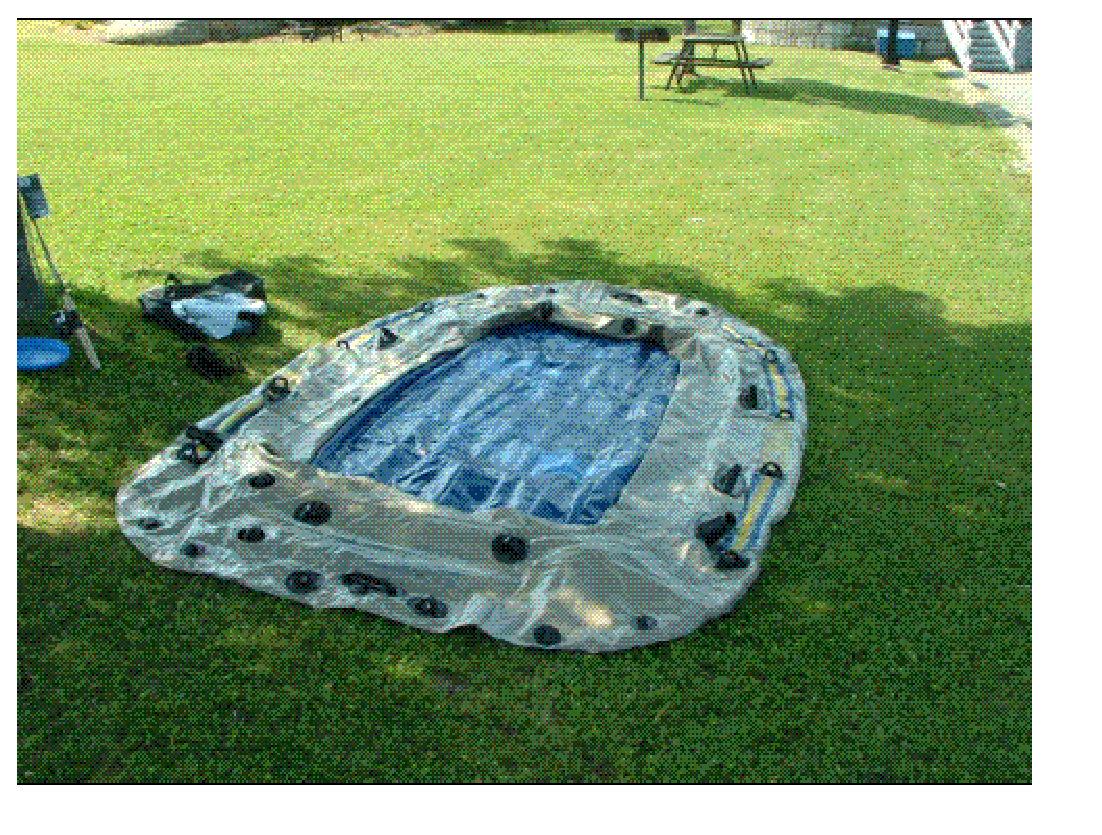
\epsfig{file=fig1.eps,width=3.5in}
Which one of the following is missing in it?
 
 
\noindent{\textbf{\large{
A.}}}
Lawn
 
 
\noindent{\textbf{\large{
B.}}}
An air-boat
 
 
\noindent{\textbf{\large{
C.}}}
A truck
 
 
\noindent{\textbf{\large{
D.}}}
An airplane
 
 
\noindent{\textbf{\large{
E.}}}
A frisbee
 
 
\noindent{\textbf{\large{
F.}}}
  Not any of aboves.
 
 
\noindent\vspace{0.05in}{\textbf{\Large{Auto-answer:}}}
 
 
\noindent{\textbf{\large{
C.}}}
A truck
 
 
\noindent{\textbf{\large{
D.}}}
An airplane
 
 
\noindent\vspace{0.05in}{\textbf{\Large{End of auto-answer.}}}
 
 
 
\vspace{0.3in}
   
   
\noindent{\textbf{\Large{Total numbers: }}}
   
   
\noindent\begin{tabular}{|l|l|l|l|l|l|l|}
 \hline
Inputs & Calculates & Choices & Layers & Matches & Answer & Solution \\ \hline
           0 & 
           0 & 
           6
  simple  
  & 
           6 & 
           0 & 
  yes & 
  no 
  \\ \hline
 \end{tabular}
   
   
   
   
\noindent\vspace{0.1in}{\textbf{\Large{Calculated values:}}}
   
   
   
   
\noindent\vspace{0.1in}\hspace{-0.08in} {\textbf{\Large{All inputs: }}}
   
   
   
   
\vspace{0.3in}
{\textbf{\LARGE{You have done all the above? A very good beginning, please go ahead.}}}
More constants the
Mass of electron
$m_e$$ =
9.109390 \times 10^{-31} $
kg
,
Universal gas constant
$R$$ =
8.315 $
J/(mol$\cdot $K)
,
$e$$ =
1.60217733 \times 10^{-19} $
C
, and
$m_p$$ =
1.6726231 \times 10^{-27} $
kg
%
may be very helpful.
\vspace{0.3in}
   
   
  
\vspace{0.2in}
  
{\textbf{\Large{QUESTION
34.2 
 (          2,          2,          2)
}}}
  
  
 
An object is subjected to an external net force $\mathbf{f}=(
50.000 ,
6.0000,
-5000.0  )N$. Its mass is known as
$m= % 
50.0000  kg$. Please choose the correct accelaration
from the following choices.
 
 
 
\noindent{\textbf{\large{
A.}}}
The accelaration is
$(
1.0000ms^{-2},
1555.2km/h^2,
443.97ms^{-2}
).
$
 
 
\noindent{\textbf{\large{
B.}}}
The accelaration is
$(
2.8752ms^{-2},
7233.3km/h^2,
-100.00ms^{-2}
).
$
 
 
\noindent{\textbf{\large{
C.}}}
The accelaration is
$(
1.0000ms^{-2},
1555.2km/h^2,
-100.00ms^{-2}
).
$
 
 
\noindent{\textbf{\large{
D.}}}
The accelaration is
$(
2.8752ms^{-2},
1555.2km/h^2,
443.97ms^{-2}
).
$
 
 
\noindent{\textbf{\large{
E.}}}
The accelaration is
$(
1.0000ms^{-2},
7233.3km/h^2,
-100.00ms^{-2}
).
$
 
 
\noindent{\textbf{\large{
F.}}}
The accelaration is
$(
2.8752ms^{-2},
1555.2km/h^2,
-100.00ms^{-2}
).
$
 
 
\noindent{\textbf{\large{
G.}}}
 None of these.
 
 
\noindent\vspace{0.05in}{\textbf{\Large{Auto-answer:}}}
 
 
\noindent{\textbf{\large{
C.}}}
The accelaration is
$(
1.0000ms^{-2},
1555.2km/h^2,
-100.00ms^{-2}
).
$
 
 
\noindent\vspace{0.05in}{\textbf{\Large{End of auto-answer.}}}
 
 
 
 
 
 
\noindent\vspace{0.1in}{\textbf{\Large{Solution: }}}
 
 

We will use the Newton's Second Law:
 
\[
\mathbf{f}=m\mathbf{a}.
\]
 
Since $\mathbf{f}=( % 
50.000,  % 
6.0000,  % 
-5000.0 )N$
and $m= % 
50.0000kg$, bring them into the above equation, then we get
 
\begin{eqnarray*}
\mathbf{a}&=&\frac{\mathbf{f}}m  \\
&=&\frac{(
50.000 ,
6.0000 ,
-5000.0 )N
}{ % 
50.0000 kg}  \\
&=&(
1.0000 ,
.12000,
-100.00
)ms^{-2} \\
&=&(
12960. ,
1555.2 ,
-1.2960 \times 10^{6}
)km/h^2.
\end{eqnarray*}
 
 
 
\noindent\vspace{0.1in}{\textbf{\Large{End of Solution.}}}
 
 

 
\vspace{0.3in}
   
   
\noindent{\textbf{\Large{Total numbers: }}}
   
   
\noindent\begin{tabular}{|l|l|l|l|l|l|l|}
 \hline
Inputs & Calculates & Choices & Layers & Matches & Answer & Solution \\ \hline
           4 & 
           6 & 
           7
  & 
           3 & 
           0 & 
  yes & 
  yes 
  \\ \hline
 \end{tabular}
   
   
   
   
\noindent\vspace{0.1in}{\textbf{\Large{Calculated values:}}}
   
   
  
  
\noindent\begin{tabular}{|l|l|l|l|}
\hline
 Sequential & Type & Accuracy & Calculated \\ 
\hline
 
 
  Calculated $           1$ & real & $           5 $ & 
 $ 1.0000 $ 
 \\  \hline  
 
 
  Calculated $           2$ & real & $           5 $ & 
 $ .12000 $ 
 \\  \hline  
 
 
  Calculated $           3$ & real & $           5 $ & 
 $ -100.00 $ 
 \\  \hline  
 
 
  Calculated $           4$ & real & $           5 $ & 
 $ 12960. $ 
 \\  \hline  
 
 
  Calculated $           5$ & real & $           5 $ & 
 $ 1555.2 $ 
 \\  \hline  
 
 
  Calculated $           6$ & real & $           5 $ & 
 $ -1.2960 \times 10^{6} $ 
 \\  \hline  
 \end{tabular}
   
   
   
   
\noindent\vspace{0.1in}\hspace{-0.08in} {\textbf{\Large{All inputs: }}}
   
   
  
  
\noindent\begin{tabular}{|l|l|l|l|l|}
\hline
 Sequential & Type & Accuracy & Three inputs & Generated \\ 
\hline
 
 
  INPUT $           1$ & real & $          -3 $ & $
 20.000
  $ & \\
  & & &  $
 101.000
  $ & \\
  & & &  $
 10.000
 $ & $ 50.000 $ 
 \\  \hline  
 
 
  INPUT $           2$ & real & $          -4 $ & $
 2.0000
  $ & \\
  & & &  $
 10.1000
  $ & \\
  & & &  $
 1.0000
 $ & $ 6.0000 $ 
 \\  \hline  
 
 
  INPUT $           3$ & real & $          -1 $ & $
 -2000.0
  $ & \\
  & & &  $
 -10001.0
  $ & \\
  & & &  $
 -1000.0
 $ & $ -5000.0 $ 
 \\  \hline  
 \end{tabular}
   
   
  
  
\noindent\begin{tabular}{|l|l|l|l|l|}
\hline
 Sequential & Type & Accuracy & Three inputs & Generated \\ 
\hline
 
 
  INPUT $           4$ & real & $          -4 $ & $
 50.0000
  $ & \\
  & & &  $
 60.1000
  $ & \\
  & & &  $
 2.0000
 $ & $ 50.0000 $ 
 \\  \hline  
 \end{tabular}
   
   
  
\vspace{0.2in}
  
{\textbf{\Large{QUESTION
34.3 
 (          1,          1,          1)
}}}
  
  


\noindent\vspace{0.05in}{\textbf{\Large{Abstract:}}}
This is a simple Newton's Second Law calculation multi-choice problem.  
\noindent\vspace{0.05in}{\textbf{\Large{end of abstract.}}}


 
 
An object is subjected to an external net force $\mathbf{f}=
(40.0 , 10.0 , -8000.0) N$.
Its mass is known as $m= % 
56.0000 kg$. Please choose the
correct accelaration from the following choices.
 
 
 
\noindent{\textbf{\large{
A.}}}
The accelaration is $  %
(
-2.32,
.18,
-545.73)
ms^{-2} $.
 
 
\noindent{\textbf{\large{
B.}}}
The accelaration is $  %
(
.714,
.18,
-545.73)
ms^{-2} $.
 
 
\noindent{\textbf{\large{
C.}}}
The accelaration is $  %
(
.714,
-.68,
-545.73)
ms^{-2} $.
 
 
\noindent{\textbf{\large{
D.}}}
The accelaration is $  %
(
-2.32,
.18,
-142.86)
ms^{-2} $.
 
 
\noindent{\textbf{\large{
E.}}}
The accelaration is $  %
(
-2.32,
-.68,
-545.73)
ms^{-2} $.
 
 
\noindent{\textbf{\large{
F.}}}
The accelaration is $  %
(
-2.32,
-.68,
-142.86)
ms^{-2} $.
 
 
\noindent{\textbf{\large{
G.}}}
The accelaration is $  %
(
.714,
.18,
-142.86)
ms^{-2} $.
 
 
\noindent{\textbf{\large{
H.}}}
The accelaration is $  %
(
.714,
-.68,
-142.86)
ms^{-2} $.
 
 
\noindent\vspace{0.05in}{\textbf{\Large{Auto-answer:}}}
 
 
\noindent{\textbf{\large{
G.}}}
The accelaration is $  %
(
.714,
.18,
-142.86)
ms^{-2} $.
 
 
\noindent\vspace{0.05in}{\textbf{\Large{End of auto-answer.}}}
 
 
 
 
 
\noindent\vspace{0.05in}{\textbf{\Large{Answer:}}}
 
 

The correct answer from the choices is


\noindent{\textbf{\large{
G.}}}
The accelaration is $  %
(
.714,
.18,
-142.86)
ms^{-2} $.
 
 
 
\noindent\vspace{0.05in}{\textbf{\Large{End of Answer.}}}
 
 

 
 
 
\noindent\vspace{0.1in}{\textbf{\Large{Solution: }}}
 
 

We will use the Newton's Second Law:
 
\[
\mathbf{f}=m\mathbf{a}.
\]
 
Since $\mathbf{f}= % 
(40.0 , 10.0 , -8000.0) N$
and $m= % 
56.0000kg$, bring them into the above equation, then we get
 
\begin{eqnarray*}
\mathbf{a}&=&\frac{\mathbf{f}}m  \\
&=&\frac{ % 
(40.0 , 10.0 , -8000.0) N}{ % 
56.0000kg}  \\
&=& % 
(.714 , .18 , -142.86) ms^{-2}
\end{eqnarray*}
 
 
 
\noindent\vspace{0.1in}{\textbf{\Large{End of Solution.}}}
 
 

 
\vspace{0.3in}
   
   
\noindent{\textbf{\Large{Total numbers: }}}
   
   
\noindent\begin{tabular}{|l|l|l|l|l|l|l|}
 \hline
Inputs & Calculates & Choices & Layers & Matches & Answer & Solution \\ \hline
           2 & 
           1 & 
           8
  & 
           3 & 
           0 & 
  yes & 
  yes 
  \\ \hline
 \end{tabular}
   
   
   
   
\noindent\vspace{0.1in}{\textbf{\Large{Calculated values:}}}
   
   
  
  
\noindent\begin{tabular}{|l|l|l|l|}
\hline
 Sequential & Type & Accuracy & Calculated \\ 
\hline
 
 
  Calculated $           1$ & vector &  
  $           3 $ 
 &  $ .714 $ 
 \\    
  & & 
  $           2 $ 
 &  $ .18 $ 
 \\    
  & & 
  $           5 $ 
 &  $ -142.86 $ 
 \\  \hline  
 \end{tabular}
   
   
   
   
\noindent\vspace{0.1in}\hspace{-0.08in} {\textbf{\Large{All inputs: }}}
   
   
  
  
\noindent\begin{tabular}{|l|l|l|l|l|}
\hline
 Sequential & Type & Accuracy & Three inputs & Generated \\ 
\hline
 
 
  INPUT $           1$ & vector & $          -1 $ & $
20.0
  $ & \\
  & & & $
101.0
  $ & \\
  & & & $
10.0
$ & $ 40.0 $ 
  \\
  & & $          -1 $ & $
2.0
  $ & \\
  & & & $
10.1
  $ & \\
  & & & $
1.0
$ & $ 10.0 $ 
  \\
  & & $          -1 $ & $
-2000.0
  $ & \\
  & & & $
-10001.0
  $ & \\
  & & & $
-1000.0
$ & $ -8000.0 $ 
 \\  \hline  
 
 
  INPUT $           2$ & real & $          -4 $ & $
 50.0000
  $ & \\
  & & &  $
 60.1000
  $ & \\
  & & &  $
 2.0000
 $ & $ 56.0000 $ 
 \\  \hline  
 \end{tabular}
   
   
  
\vspace{0.2in}
  
{\textbf{\Large{QUESTION
34.4 
 (          3,          3,          3)
}}}
  
  
Please choose the correct one from the following statements:
 
 
\noindent{\textbf{\large{
A.}}}
Canada has  %
36 provinces and  %
35 territories.
 
 
\noindent{\textbf{\large{
B.}}}
Canada has  %
34 provinces and  %
39 territories.
 
 
\noindent{\textbf{\large{
C.}}}
Canada has  %
37 provinces and  %
37 territories.
 
 
\noindent{\textbf{\large{
D.}}}
Canada has  %
33 provinces and  %
38 territories.
 
 
\noindent{\textbf{\large{
E.}}}
Canada has  %
10 provinces and  %
3 territories.
 
 
\noindent{\textbf{\large{
F.}}}
 None of above.
 
 
\noindent\vspace{0.05in}{\textbf{\Large{Auto-answer:}}}
 
 
\noindent{\textbf{\large{
E.}}}
Canada has  %
10 provinces and  %
3 territories.
 
 
\noindent\vspace{0.05in}{\textbf{\Large{End of auto-answer.}}}
 
 
   
   
\noindent{\textbf{\Large{Total numbers: }}}
   
   
\noindent\begin{tabular}{|l|l|l|l|l|l|l|}
 \hline
Inputs & Calculates & Choices & Layers & Matches & Answer & Solution \\ \hline
           0 & 
          20 & 
           6
  simple  
  & 
           6 & 
           0 & 
  yes & 
  no 
  \\ \hline
 \end{tabular}
   
   
   
   
\noindent\vspace{0.1in}{\textbf{\Large{Calculated values:}}}
   
   
  
  
\noindent\begin{tabular}{|l|l|l|l|}
\hline
 Sequential & Type & Accuracy & Calculated \\ 
\hline
 
 
  Calculated $           1$ & integer &  & 
  $ 10 $ 
 \\  \hline  
 
 
  Calculated $           2$ & integer &  & 
  $ 3 $ 
 \\  \hline  
 
 
  Calculated $           3$ & integer &  & 
  $ 23 $ 
 \\  \hline  
 
 
  Calculated $           4$ & integer &  & 
  $ 24 $ 
 \\  \hline  
 
 
  Calculated $           5$ & integer &  & 
  $ 25 $ 
 \\  \hline  
 
 
  Calculated $           6$ & integer &  & 
  $ 26 $ 
 \\  \hline  
 
 
  Calculated $           7$ & integer &  & 
  $ 27 $ 
 \\  \hline  
 
 
  Calculated $           8$ & integer &  & 
  $ 28 $ 
 \\  \hline  
 
 
  Calculated $           9$ & integer &  & 
  $ 29 $ 
 \\  \hline  
 
 
  Calculated $          10$ & integer &  & 
  $ 30 $ 
 \\  \hline  
 \end{tabular}
   
   
  
  
\noindent\begin{tabular}{|l|l|l|l|}
\hline
 Sequential & Type & Accuracy & Calculated \\ 
\hline
 
 
  Calculated $          11$ & integer &  & 
  $ 31 $ 
 \\  \hline  
 
 
  Calculated $          12$ & integer &  & 
  $ 32 $ 
 \\  \hline  
 
 
  Calculated $          13$ & integer &  & 
  $ 33 $ 
 \\  \hline  
 
 
  Calculated $          14$ & integer &  & 
  $ 34 $ 
 \\  \hline  
 
 
  Calculated $          15$ & integer &  & 
  $ 35 $ 
 \\  \hline  
 
 
  Calculated $          16$ & integer &  & 
  $ 36 $ 
 \\  \hline  
 
 
  Calculated $          17$ & integer &  & 
  $ 37 $ 
 \\  \hline  
 
 
  Calculated $          18$ & integer &  & 
  $ 38 $ 
 \\  \hline  
 
 
  Calculated $          19$ & integer &  & 
  $ 39 $ 
 \\  \hline  
 
 
  Calculated $          20$ & integer &  & 
  $ 40 $ 
 \\  \hline  
 \end{tabular}
   
   
   
   
\noindent\vspace{0.1in}\hspace{-0.08in} {\textbf{\Large{All inputs: }}}
   
   
  
\vspace{0.2in}
  
{\textbf{\Large{QUESTION
34.5 
 (          5,          5,          5)
}}}
  
  
If any one of the following statements is correct, please fill the box ahead of it with $T$ .
If wrong, fill with $F$.
 
\noindent\begin{tabular}{|l|l|}\hline Your&\hspace{.2in} \\ answer&\hspace{.2in} \\ \hline \end{tabular}
1. $ % 
97$ is an  % 
odd number.
 
\noindent\begin{tabular}{|l|l|}\hline Your&\hspace{.2in} \\ answer&\hspace{.2in} \\ \hline \end{tabular}
2.  % 
Kingston is in  % 
Ontario province.
 
\noindent\begin{tabular}{|l|l|}\hline Your&\hspace{.2in} \\ answer&\hspace{.2in} \\ \hline \end{tabular}
3.  % 
$\mathbf{F}=m\mathbf{a}$ is a mathmatical form of
the Newton's Second Law.
 
 
 
\noindent\vspace{0.05in}{\textbf{\Large{Answer:}}}
 
 

 
\noindent\begin{tabular}{|l|l|}\hline The correct & \\
          answer &  % 
$T$ \\ \hline \end{tabular}
1. $ % 
97$ is an  % 
odd number.
 
\noindent\begin{tabular}{|l|l|}\hline The correct & \\
          answer &  % 
$T$ \\ \hline \end{tabular}
2.  % 
Kingston is in  % 
Ontario province.
 
\noindent\begin{tabular}{|l|l|}\hline The correct & \\
          answer &  % 
$T$ \\ \hline \end{tabular}
3.  % 
$\mathbf{F}=m\mathbf{a}$ is a mathmatical form of  % 
the Newton's Second Law.
 
 
 
\noindent\vspace{0.05in}{\textbf{\Large{End of Answer.}}}
 
 

 
\vspace{0.3in}
   
   
\noindent{\textbf{\Large{Total numbers: }}}
   
   
\noindent\begin{tabular}{|l|l|l|l|l|l|l|}
 \hline
Inputs & Calculates & Choices & Layers & Matches & Answer & Solution \\ \hline
           6 & 
           3 & 
           0
  & 
           0 & 
           0 & 
  yes & 
  no 
  \\ \hline
 \end{tabular}
   
   
   
   
\noindent\vspace{0.1in}{\textbf{\Large{Calculated values:}}}
   
   
  
  
\noindent\begin{tabular}{|l|l|l|l|}
\hline
 Sequential & Type & Accuracy & Calculated \\ 
\hline
 
 
  Calculated $           1$ & string & $           1 $ ( $          2 $ strings)
 : 
 & $T$
 \\  \hline  
 
 
  Calculated $           2$ & string & $           1 $ ( $          2 $ strings)
 : 
 & $T$
 \\  \hline  
 
 
  Calculated $           3$ & string & $           1 $ ( $          2 $ strings)
 : 
 & $T$
 \\  \hline  
 \end{tabular}
   
   
   
   
\noindent\vspace{0.1in}\hspace{-0.08in} {\textbf{\Large{All inputs: }}}
   
   
  
  
\noindent\begin{tabular}{|l|l|l|l|l|}
\hline
 Sequential & Type & Accuracy & Three inputs & Generated \\ 
\hline
 
 
  INPUT $           1$ & integer &  & $
 1
 , 
 100
 , 
 1
 $ & $ 97 $ 
 \\  \hline  
 
 
  INPUT $           2$ & string & & 
 even & 
  \\
  & & & 
 odd & 
  $ <-- $ 
 \\  \hline  
 
 
  INPUT $           3$ & string & & 
 Toronto & 
  \\
  & & & 
 Kingston & 
  $ <-- $ 
  \\
  & & & 
 Montreal & 
  \\
  & & & 
 Hull & 
 \\  \hline  
 \end{tabular}
   
   
  
  
\noindent\begin{tabular}{|l|l|l|l|l|}
\hline
 Sequential & Type & Accuracy & Three inputs & Generated \\ 
\hline
 
 
  INPUT $           4$ & string & & 
 Ontario & 
  $ <-- $ 
  \\
  & & & 
 Quebec & 
 \\  \hline  
 
 
  INPUT $           5$ & string & & 
 $\mathbf{F}=m\mathbf{a}$ & 
  $ <-- $ 
  \\
  & & & 
 $\left| \mathbf{F}\right| =Gm_1m_2r^{-2}$ & 
 \\  \hline  
 
 
  INPUT $           6$ & string & & 
 the Newton's Second Law & 
  $ <-- $ 
  \\
  & & & 
 Newton's Law of Universal Gravitation & 
 \\  \hline  
 \end{tabular}
   
   
  
\vspace{0.2in}
  
{\textbf{\Large{QUESTION
34.6 
 (          4,          4,          4)
}}}
  
  
Considering case-insensitivity, please match the following same strings.
  
  
\begin{tabular}{|l|l|l|}
 \hline
 Column Left & Column Right  & Your choinces \\ 
 \hline
{\textbf{\large{
A.}}}
C
  & 
YJH
 & 
 \\ 
 \hline
{\textbf{\large{
B.}}}
A
  & 
a
 & 
 \\ 
 \hline
{\textbf{\large{
C.}}}
B
  & 
c
 & 
 \\ 
 \hline
{\textbf{\large{
D.}}}
asdf(:)
  & 
ASDF(:)
 & 
 \\ 
 \hline
{\textbf{\large{
E.}}}
yjh
  & 
b
 & 
 \\ 
 \hline
 \end{tabular}
  
  
 
 
\noindent\vspace{0.05in}{\textbf{\Large{Auto-answer:}}}
  
  
\begin{tabular}{|l|l|l|}
 \hline
 Column Left & Column Right  & Answers       \\ 
 \hline
{\textbf{\large{
A.}}}
C
  & 
YJH
 & 
{\textbf{\large{
E.}}}
 \\ 
 \hline
{\textbf{\large{
B.}}}
A
  & 
a
 & 
{\textbf{\large{
B.}}}
 \\ 
 \hline
{\textbf{\large{
C.}}}
B
  & 
c
 & 
{\textbf{\large{
A.}}}
 \\ 
 \hline
{\textbf{\large{
D.}}}
asdf(:)
  & 
ASDF(:)
 & 
{\textbf{\large{
D.}}}
 \\ 
 \hline
{\textbf{\large{
E.}}}
yjh
  & 
b
 & 
{\textbf{\large{
C.}}}
 \\ 
 \hline
 \end{tabular}
  
  
 
 
\noindent\vspace{0.05in}{\textbf{\Large{End of auto-answer.}}}
 
 
 
   
   
\noindent{\textbf{\Large{Total numbers: }}}
   
   
\noindent\begin{tabular}{|l|l|l|l|l|l|l|}
 \hline
Inputs & Calculates & Choices & Layers & Matches & Answer & Solution \\ \hline
           2 & 
           1 & 
           0
  & 
          16 & 
           5 & 
  yes & 
  no 
  \\ \hline
 \end{tabular}
   
   
   
   
\noindent\vspace{0.1in}{\textbf{\Large{Calculated values:}}}
   
   
  
  
\noindent\begin{tabular}{|l|l|l|l|}
\hline
 Sequential & Type & Accuracy & Calculated \\ 
\hline
 
 
  Calculated $           1$ & integer &  & 
  $ 3 $ 
 \\  \hline  
 \end{tabular}
   
   
   
   
\noindent\vspace{0.1in}\hspace{-0.08in} {\textbf{\Large{All inputs: }}}
   
   
  
  
\noindent\begin{tabular}{|l|l|l|l|l|}
\hline
 Sequential & Type & Accuracy & Three inputs & Generated \\ 
\hline
 
 
  INPUT $           1$ & integer &  & $
 2
 , 
 8
 , 
 2
 $ & $ 6 $ 
 \\  \hline  
 
 
  INPUT $           2$ & integer &  & $
 2
 , 
 3
 , 
 2
 $ & $ 2 $ 
 \\  \hline  
 \end{tabular}
   
   
   
   
\vspace{0.3in}
{\textbf{\LARGE{You have done all the above? Excellent! Not much left, please continue.}}}
\vspace{0.3in}
   
   
  
\vspace{0.2in}
  
{\textbf{\Large{QUESTION
34.7 
 (          8,         15,         60)
}}}
  
  
 
$ \left( \begin{array}{ccccccccc}
           5 & 
           5 & 
           4 & 
           6 \\ 
           6 & 
           4 & 
           7 & 
           5 \\ 
           7 & 
           7 & 
           7 & 
           7
\end{array}\right) \times
\left( \begin{array}{c}
           2 \\ 
           2 \\ 
           2 \\ 
           2
\end{array}\right) $ =?
 
 
$  % 
 \left( \begin{array}
 {
 c
 c
 }
                    \zeta & 
 \varepsilon \\ 
 \gamma & 
 \Gamma \\ 
 \Theta & 
 \varepsilon \\ 
 \gamma & 
                    \zeta
 \end{array} \right)
 \left( \begin{array}
 {
 c
 }
 \beta \\ 
 \beta
 \end{array} \right)
$ =?
 
 
 
\noindent\vspace{0.05in}{\textbf{\Large{Answer:}}}
 
 

 
$\left( \begin{array}{ccccccccccccccc}
           5 & 
           5 & 
           4 & 
           6 \\ 
           6 & 
           4 & 
           7 & 
           5 \\ 
           7 & 
           7 & 
           7 & 
           7
\end{array}\right) \times
\left( \begin{array}{c}
           2 \\ 
           2 \\ 
           2 \\ 
           2
\end{array}\right)  =
\left( \begin{array}{c}
          40 \\ 
          44 \\ 
          56
\end{array}\right)  $
 
$  % 
 \left( \begin{array}
 {
 c
 c
 }
                    \zeta & 
 \varepsilon \\ 
 \gamma & 
 \Gamma \\ 
 \Theta & 
 \varepsilon \\ 
 \gamma & 
                    \zeta
 \end{array} \right)
 \left( \begin{array}
 {
 c
 }
 \beta \\ 
 \beta
 \end{array} \right)
=
  \left( \begin{array}
 {
 c
 }
                    \zeta \times  \beta   +  \varepsilon \times  \beta \\ 
 \gamma \times  \beta   +  \Gamma \times  \beta \\ 
 \Theta \times  \beta   +  \varepsilon \times  \beta \\ 
 \gamma \times  \beta   +                     \zeta \times  \beta
 \end{array} \right)
$
 
 
 
\noindent\vspace{0.05in}{\textbf{\Large{End of Answer.}}}
 
 

 
 
 
\noindent\vspace{0.1in}{\textbf{\Large{Solution: }}}
 
 

 
 
\noindent\vspace{0.1in}{\textbf{\Large{End of Solution.}}}
 
 

 
\vspace{0.3in}
   
   
\noindent{\textbf{\Large{Total numbers: }}}
   
   
\noindent\begin{tabular}{|l|l|l|l|l|l|l|}
 \hline
Inputs & Calculates & Choices & Layers & Matches & Answer & Solution \\ \hline
           4 & 
           2 & 
           0
  & 
           0 & 
           0 & 
  yes & 
  yes 
  \\ \hline
 \end{tabular}
   
   
   
   
\noindent\vspace{0.1in}{\textbf{\Large{Calculated values:}}}
   
   
  
  
\noindent\begin{tabular}{|l|l|l|l|}
\hline
 Sequential & Type & Accuracy & Calculated \\ 
\hline
 
 
  Calculated $           1$ & i-matrix &  & 
 (size:           3 by           1)
 \\  \hline  
 \end{tabular}
   
   
$\begin{array}{
 c
 }
          40 \\ 
          44 \\ 
          56
 \end{array}  $ 
  
  
\noindent\begin{tabular}{|l|l|l|l|}
\hline
 Sequential & Type & Accuracy & Calculated \\ 
\hline
 
 
  Calculated $           2$ & s-matrix & & 
 (size:           4 by           1)
 \\  \hline  
 \end{tabular}
   
   
 $   \left( \begin{array}
 {
 c
 }
                    \zeta \times  \beta   +  \varepsilon \times  \beta \\ 
 \gamma \times  \beta   +  \Gamma \times  \beta \\ 
 \Theta \times  \beta   +  \varepsilon \times  \beta \\ 
 \gamma \times  \beta   +                     \zeta \times  \beta
 \end{array} \right) $ 
   
   
\noindent\vspace{0.1in}\hspace{-0.08in} {\textbf{\Large{All inputs: }}}
   
   
  
  
\noindent\begin{tabular}{|l|l|l|l|l|}
\hline
 Sequential & Type & Accuracy & Three inputs & Generated \\ 
\hline
 
 
  INPUT $           1$ & i-matrix &  & $
 4
 , 
 7
 , 
 1
 $ & (size:           3 by           4)
 \\  \hline  
 \end{tabular}
   
   
 $\begin{array}{
 c
 c
 c
 c
 }
           5 & 
           5 & 
           4 & 
           6 \\ 
           6 & 
           4 & 
           7 & 
           5 \\ 
           7 & 
           7 & 
           7 & 
           7
\end{array}  $ 
  
  
\noindent\begin{tabular}{|l|l|l|l|l|}
\hline
 Sequential & Type & Accuracy & Three inputs & Generated \\ 
\hline
 
 
  INPUT $           2$ & i-matrix &  & $
 2
 , 
 2
 , 
 1
 $ & (size:           4 by           1)
 \\  \hline  
 \end{tabular}
   
   
 $\begin{array}{
 c
 }
           2 \\ 
           2 \\ 
           2 \\ 
           2
\end{array}  $ 
  
  
\noindent\begin{tabular}{|l|l|l|l|l|}
\hline
 Sequential & Type & Accuracy & Three inputs & Generated \\ 
\hline
 
 
  INPUT $           3$ & s-matrix & & 
 $  \alpha $ & 
  \\
  & & & 
 $  \beta $ & 
  \\
  & & & 
 $  \gamma $ & 
  \\
  & & & 
 $  \delta $ & 
  \\
  & & & 
 $  \epsilon $ & 
  \\
  & & & 
 $  \varepsilon $ & 
  \\
  & & & 
 $                     \zeta $ & 
  \\
  & & & 
 $  \eta $ & 
  \\
  & & & 
 $  \rho $ & 
  \\
  & & & 
 $  \sigma $ & 
  \\
  & & & 
 $  \Gamma $ & 
  \\
  & & & 
 $  \Delta $ & 
  \\
  & & & 
 $  \Theta $ & 
  \\
  & & & 
 $  \Lambda $ & 
  \\
  & & & 
 $                     \Xi $ & 
  \\
  & & & 
 $  \Upsilon $ & 
  \\
  & & & 
 $  \Phi $ & 
  \\
  & & & 
 $  \Psi $ & 
  \\
  & & & 
 $  \Omega $ & 
  (size:           4 by           2)
 \\  \hline  
 \end{tabular}
   
   
 $  \left( \begin{array}
 {
 c
 c
 }
                    \zeta & 
 \varepsilon \\ 
 \gamma & 
 \Gamma \\ 
 \Theta & 
 \varepsilon \\ 
 \gamma & 
                    \zeta
 \end{array} \right) $ 
  
  
\noindent\begin{tabular}{|l|l|l|l|l|}
\hline
 Sequential & Type & Accuracy & Three inputs & Generated \\ 
\hline
 
 
  INPUT $           4$ & s-matrix & & 
 $  \beta $ & 
  \\
  & & & 
 $  \gamma $ & 
  (size:           2 by           1)
 \\  \hline  
 \end{tabular}
   
   
 $  \left( \begin{array}
 {
 c
 }
 \beta \\ 
 \beta
 \end{array} \right) $ 
  
\vspace{0.2in}
  
{\textbf{\Large{QUESTION
34.8 
 (          7,         14,         50)
}}}
  
  
 
An object is subjected to an external net force $\mathbf{f}=
(90.0 , 9.0 , -4000.0) N$.
Its mass is known as $m= % 
54.0 kg$.
Please choose the correct accelaration from the following choices.
 
 
\noindent{\textbf{\large{
A.}}}
  The accelaration is $  %
(
1.67,
.17,
264.68)
ms^{-2} $.
 
 
\noindent{\textbf{\large{
B.}}}
  The accelaration is $  %
(
1.67,
-.50,
-74.074)
ms^{-2} $.
 
 
\noindent{\textbf{\large{
C.}}}
  The accelaration is $  %
(
1.67,
.17,
-74.074)
ms^{-2} $.
 
 
\noindent{\textbf{\large{
D.}}}
  The accelaration is $  %
(
7.96,
.17,
264.68)
ms^{-2} $.
 
 
\noindent\vspace{0.05in}{\textbf{\Large{Auto-answer:}}}
 
 
\noindent{\textbf{\large{
C.}}}
  The accelaration is $  %
(
1.67,
.17,
-74.074)
ms^{-2} $.
 
 
\noindent\vspace{0.05in}{\textbf{\Large{End of auto-answer.}}}
 
 
 
 
 
\noindent\vspace{0.1in}{\textbf{\Large{Solution: }}}
 
 

We will use the Newton's Second Law:
 
\[
\mathbf{f}=m\mathbf{a}.
\]
 
Since $\mathbf{f}= % 
(90.0 , 9.0 , -4000.0) N$
and $m= % 
54.0kg$, bring them into the above equation, then we get
 
\begin{eqnarray*}
\mathbf{a}&=&\frac{\mathbf{f}}m  \\
&=&\frac{ % 
(90.0 , 9.0 , -4000.0) N}{ % 
54.0kg}  \\
&=& % 
(1.67 , .17 , -74.074) ms^{-2}
\end{eqnarray*}
 
 
 
\noindent\vspace{0.1in}{\textbf{\Large{End of Solution.}}}
 
 

 
 
\vspace{0.3in}
   
   
\noindent{\textbf{\Large{Total numbers: }}}
   
   
\noindent\begin{tabular}{|l|l|l|l|l|l|l|}
 \hline
Inputs & Calculates & Choices & Layers & Matches & Answer & Solution \\ \hline
           2 & 
           1 & 
           4
  & 
           3 & 
           0 & 
  yes & 
  yes 
  \\ \hline
 \end{tabular}
   
   
   
   
\noindent\vspace{0.1in}{\textbf{\Large{Calculated values:}}}
   
   
  
  
\noindent\begin{tabular}{|l|l|l|l|}
\hline
 Sequential & Type & Accuracy & Calculated \\ 
\hline
 
 
  Calculated $           1$ & vector &  
  $           3 $ 
 &  $ 1.67 $ 
 \\    
  & & 
  $           2 $ 
 &  $ .17 $ 
 \\    
  & & 
  $           5 $ 
 &  $ -74.074 $ 
 \\  \hline  
 \end{tabular}
   
   
   
   
\noindent\vspace{0.1in}\hspace{-0.08in} {\textbf{\Large{All inputs: }}}
   
   
  
  
\noindent\begin{tabular}{|l|l|l|l|l|}
\hline
 Sequential & Type & Accuracy & Three inputs & Generated \\ 
\hline
 
 
  INPUT $           1$ & vector & $          -1 $ & $
20.0
  $ & \\
  & & & $
101.0
  $ & \\
  & & & $
10.0
$ & $ 90.0 $ 
  \\
  & & $          -1 $ & $
2.0
  $ & \\
  & & & $
10.1
  $ & \\
  & & & $
1.0
$ & $ 9.0 $ 
  \\
  & & $          -1 $ & $
-2000.0
  $ & \\
  & & & $
-10001.0
  $ & \\
  & & & $
-1000.0
$ & $ -4000.0 $ 
 \\  \hline  
 
 
  INPUT $           2$ & real & $          -1 $ & $
 50.0
  $ & \\
  & & &  $
 60.1
  $ & \\
  & & &  $
 2.0
 $ & $ 54.0 $ 
 \\  \hline  
 \end{tabular}
   
   
  
\vspace{0.2in}
  
{\textbf{\Large{QUESTION
34.9 
 (          9,         16,         70)
}}}
  
  


\noindent\vspace{0.05in}{\textbf{\Large{Abstract:}}}
Quadratic Equation constructed from the following first two random (input) integers as roots,  
which of course should not show in the exam papers.  
\noindent\vspace{0.05in}{\textbf{\Large{end of abstract.}}}


 
 
% First root
% Second root

 
Please solve the following equation:
\begin{eqnarray*}
-5 \times x^2  % 
+  % 
205
                 \times x    % 
-2100 =0
\end{eqnarray*}
 
 
 
\noindent\vspace{0.05in}{\textbf{\Large{Answer:}}}
 
 

21,  % 
20
 
 
 
\noindent\vspace{0.05in}{\textbf{\Large{End of Answer.}}}
 
 

 
 
 
\noindent\vspace{0.1in}{\textbf{\Large{Solution: }}}
 
 

Roots to the equation
\begin{eqnarray*}
-5 \times x^2  % 
+  % 
205
                 \times x    % 
-2100 =0
\end{eqnarray*}
are  % 
21 and  % 
20 .
 
Let us verity  % 
21 first:
$  % 
-5 \times x^2  % 
+  % 
205
                 \times x    % 
-2100
  = % 
-2205+( % 
4305)+( % 
-2100)
  = % 
2100+( % 
-2100)
  = % 
0
$
 
Then verity  % 
20:
$  % 
-5 \times x^2  % 
+  % 
205
                 \times x    % 
-2100
  = % 
-2000+( % 
4100)+( % 
-2100)
  = % 
2100+( % 
-2100)
  = % 
0
$
 
 
 
\noindent\vspace{0.1in}{\textbf{\Large{End of Solution.}}}
 
 

 
\vspace{0.3in}
   
   
\noindent{\textbf{\Large{Total numbers: }}}
   
   
\noindent\begin{tabular}{|l|l|l|l|l|l|l|}
 \hline
Inputs & Calculates & Choices & Layers & Matches & Answer & Solution \\ \hline
           3 & 
          13 & 
           0
  & 
           0 & 
           0 & 
  yes & 
  yes 
  \\ \hline
 \end{tabular}
   
   
   
   
\noindent\vspace{0.1in}{\textbf{\Large{Calculated values:}}}
   
   
  
  
\noindent\begin{tabular}{|l|l|l|l|}
\hline
 Sequential & Type & Accuracy & Calculated \\ 
\hline
 
 
  Calculated $           1$ & integer &  & 
  $ -5 $ 
 \\  \hline  
 
 
  Calculated $           2$ & string & $           1 $ ( $          2 $ strings)
 : 
 & +
 \\  \hline  
 
 
  Calculated $           3$ & integer &  & 
  $ 205 $ 
 \\  \hline  
 
 
  Calculated $           4$ & string & $           2 $ ( $          2 $ strings)
 : 
 & 
 \\  \hline  
 
 
  Calculated $           5$ & integer &  & 
  $ -2100 $ 
 \\  \hline  
 
 
  Calculated $           6$ & integer &  & 
  $ -2205 $ 
 \\  \hline  
 
 
  Calculated $           7$ & integer &  & 
  $ 4305 $ 
 \\  \hline  
 
 
  Calculated $           8$ & integer &  & 
  $ 2100 $ 
 \\  \hline  
 
 
  Calculated $           9$ & integer &  & 
  $ 0 $ 
 \\  \hline  
 
 
  Calculated $          10$ & integer &  & 
  $ -2000 $ 
 \\  \hline  
 \end{tabular}
   
   
  
  
\noindent\begin{tabular}{|l|l|l|l|}
\hline
 Sequential & Type & Accuracy & Calculated \\ 
\hline
 
 
  Calculated $          11$ & integer &  & 
  $ 4100 $ 
 \\  \hline  
 
 
  Calculated $          12$ & integer &  & 
  $ 2100 $ 
 \\  \hline  
 
 
  Calculated $          13$ & integer &  & 
  $ 0 $ 
 \\  \hline  
 \end{tabular}
   
   
   
   
\noindent\vspace{0.1in}\hspace{-0.08in} {\textbf{\Large{All inputs: }}}
   
   
  
  
\noindent\begin{tabular}{|l|l|l|l|l|}
\hline
 Sequential & Type & Accuracy & Three inputs & Generated \\ 
\hline
 
 
  INPUT $           1$ & integer &  & $
 -11
 , 
 30
 , 
 4
 $ & $ 21 $ 
 \\  \hline  
 
 
  INPUT $           2$ & integer &  & $
 -31
 , 
 60
 , 
 3
 $ & $ 20 $ 
 \\  \hline  
 
 
  INPUT $           3$ & integer &  & $
 -15
 , 
 15
 , 
 2
 $ & $ -5 $ 
 \\  \hline  
 \end{tabular}
   
   
   
   
   
   
 \vspace{0.2in}
Here are still some constants for use:
 
 
\noindent\begin{tabular}{|l|l|l|}
\hline
Constant & Symbol & Value \\
\hline
 
Mass of proton &
$m_p$ &
 $ 1.6726231 \times 10^{-27} $
kg \\
\hline
 
Boltzmann's constant &
$k$ &
 $ 1.381 \times 10^{-23} $
J/K \\
\hline
 
\end{tabular}
 
Thank you very much for answering these questions!
 
{\textbf{\large{Please be advised}}} that in this paper there are questions from
34.1 through
34.9.
And any one of them may contain more than one sub-question, thus the total number
of sub-questions here is around 14, of which
13 should be answered.
 
   
   
\vspace{2.0in} PAPER TAIL GENERATED.
   
   
   
   
\vspace{1.0in} 
{\textbf{\large{ *** END OF PAPER, THANKS *** }}} 
   
   
\hspace{1.0in} By: 
         239(         26,          34)
   
   
   
\vspace{0.2in}
\vspace{0.2in}
   
   
 \newpage
\setcounter{page}{1} 
   
   
 {\LARGE{STATISTICS}}
   
\vspace{0.2in}
   
 \begin{tabular}{|l|l|}
 \hline
 Initial seed for random numbers &        239 \\
\hline
 First paper number &         26 \\
\hline
 Last  paper number &         34 \\
\hline
 Total papers to be generated &          9 \\
\hline
Total marks from input file & 100.00 \\
\hline
Total actual marks & 100.00 \\
\hline
 Total lines of the input file &        915 \\
 \hline
 Total QUESTIONs in input file &         16 \\
\hline
 Total CHOOSEs in input file &          1 \\
\hline
 Total NOTEs in input file &          2 \\
\hline
 Total (big) questions in each paper &          9 \\
\hline
 Total actual (sub)questions in each paper &         14 \\
\hline
 Total (sub)questions to be answered in each paper &         13 \\
\hline
 \end{tabular}
   
   
 \newpage
   
{\LARGE{For each big question}}
   
   
\vspace{0.2in}
   
   
\noindent\hspace{-0.4in}\begin{tabular}{|l|l|l|l|l|}
\hline
 Big question & Choose? & Questions needed & Questions from & Question IDs \\ 
\hline
           1(          4,3.13
 ) &  No   & 
           1(          1,           1) &           1(          1
,3.13
 ,10.00) &           1 \\
 \hline
           2(          4,1.56
 ) &  No   & 
           1(          1,           1) &           2(          0
,1.56
 ,5.00) &           2 \\
 \hline
           3(          4,1.56
 ) &  No   & 
           1(          1,           1) &           3(          1
,1.56
 ,5.00) &           3 \\
 \hline
           4(          4,3.13
 ) &  No   & 
           1(          1,           1) &           4(          0
,3.13
 ,10.00) &           4 \\
 \hline
           5(          4,1.56
 ) &  No   & 
           1(          1,           1) &           5(          0
,1.56
 ,5.00) &           5 \\
 \hline
           6(          2,62.50
,40.00
 ) &           1 & 
           6(          5,           8) &           6(          0
,12.50
 ,5.00) &          21 \\
  & & &           7(          0
 ,12.50
 ,5.00) &          22 \\
  & & &           8(          0
 ,12.50
 ,6.00) &          23 \\
  & & &           9(          0
 ,12.50
 ,8.00) &          24 \\
  & & &          10(          1
 ,12.50
 ,5.70) &          25 \\
  & & &          11(          0
 ,12.50
 ,12.40) &          26 \\
  & & &          12(          0
 ,12.50
 ,24.50) &          27 \\
 \hline
 \end{tabular}
   
   
 \vspace{0.2in}
   
   
\noindent\hspace{-0.4in}\begin{tabular}{|l|l|l|l|l|}
\hline
 Big question & Choose? & Questions needed & Questions from & Question IDs \\ 
\hline
  & & &          13(          0
 ,12.50
 ,67.20) &          28 \\
 \hline
           7(          8,12.50
 ) &  No   & 
           1(          1,           1) &          14(          1
,12.50
 ,40.00) &          50 \\
 \hline
           8(          8,12.50
 ) &  No   & 
           1(          1,           1) &          15(          0
,12.50
 ,40.00) &          60 \\
 \hline
           9(         14,1.56
 ) &  No   & 
           1(          1,           1) &          16(          0
,1.56
 ,5.00) &          70 \\
 \hline
 \end{tabular}
 
 
\end{document}
